% 서울대학교 전기공학부 (전기컴퓨터공학부) 석사ㅡ 박사 학위논문
% LaTeX 양식 샘플
\RequirePackage{fix-cm} % documentclass 이전에 넣는다.
% oneside : 단면 인쇄용
% twoside : 양면 인쇄용
% ko : 국문 논문 작성
% master : 석사
% phd : 박사
% openright : 챕터가 홀수쪽에서 시작
\documentclass[oneside,phd]{snuthesis}

\include{snutocstyle} % SNU toc style

%%%%%%%%%%%%%%%%%%%%%%%%%%%%%%%%%%%%%%%%
%% 다른 패키지 로드
%% http://faq.ktug.or.kr/faq/pdflatex%B0%FAlatex%B5%BF%BD%C3%BB%E7%BF%EB
%% 필요에 따라 직접 수정 필요
\ifpdf
	\input glyphtounicode\pdfgentounicode=1 %type 1 font사용시
	\usepackage[pdftex,unicode]{hyperref} % delete me
	\usepackage[pdftex]{graphicx}
	\usepackage[pdftex,svgnames,table]{xcolor}
\else
	\usepackage[dvipdfmx,unicode]{hyperref} % delete me
	\usepackage[dvipdfmx]{graphicx}
	\usepackage[dvipdfmx,svgnames,table]{xcolor}
\fi
%%%%%%%%%%%%%%%%%%%%%%%%%%%%%%%%%%%%%%%%

\usepackage{lipsum} % lorem ipsum
\usepackage{alltt}
\usepackage{mathpartir}
\usepackage[utf8]{inputenc}
\usepackage[T1]{fontenc}
\usepackage{stmaryrd}
\usepackage{MinionPro}
\usepackage{MyriadPro}
\usepackage{amsmath}
\usepackage{amsthm}
\usepackage{mathtools}
\usepackage[scaled]{beramono}
\usepackage{minted}
\usepackage{cleveref}
\usepackage[shortlabels]{enumitem}
\usepackage{lscape}

\linespread{1.1}
\renewcommand{\thechapter}{\Roman{chapter}}
\counterwithout{section}{chapter}

\hyphenation{Comp-Cert}

%% \title : 22pt로 나오는 큰 제목
%% \title* : 16pt로 나오는 작은 제목
\title{Reconciling Low-Level Features of C \\ with Compiler Optimizations}
\title*{C의 저수준 기능과 컴파일러 최적화 조화시키기}

\academicko{공학}
\schoolen{COLLEGE OF ENGINEERING}
\departmenten{DEPARTMENT OF ELECTRICAL ENGINEERING AND\\ COMPUTER SCIENCE}
\departmentko{전기 컴퓨터 공학부}

%% 저자 이름 Author's(Your) name
%\author{홍길동}
%\author*{홍~길~동} % Insert space for Hangul name.
\author{Jeehoon Kang}
\author*{강~지~훈} % Same as \author.

%% 학번 Student number
\studentnumber{2013-20737}

%% 지도교수님 성함 Advisor's name
%% (?) Use Korean name for Korean professor.
%\advisor{홍길동}
%\advisor*{홍~길~동} % Insert space for Hangul name.
\advisor{Chung-Kil Hur}
\advisor*{허~충~길}

%% 학위 수여일 Graduation date
%% 표지에 적히는 날짜.
%% 학위 수여일이 아니라 논문 발간년도를 적어야 할 수도 있음.
%\graddate{2010~년~2~월}
\graddate{FEBRUARY 2019}

%% 논문 제출일 Submission date
%% (?) Use Korean date format.
\submissiondate{2019~년~1~월}

%% 논문 인준일 Approval date
%% (?) Use Korean date format.
\approvaldate{2019~년~1~월}

%% Note: 인준지의 교수님 성함은
%% 컴퓨터로 출력하지 않고, 교수님께서
%% 자필로 쓰시기도 합니다.
%% Committee members' names
\committeemembers%
{이광근}%
{허충길}%
{전병곤}%
{이재욱}%
{Derek Dreyer}
%% Length of underline
%\setlength{\committeenameunderlinelength}{7cm}

\newcommand{\jeehoon}[1]{\textbf{jeehoon: {#1}}}
\newcommand{\code}[1]{\texttt{#1}}
\newcommand{\eg}{\emph{e.g.}, }
\newcommand{\ie}{\emph{i.e.}, }
\newcommand{\etal}{\emph{et. al.} }
\newcommand{\optarrow}{\ensuremath{\rightsquigarrow}}


%%% math

\newcommand{\defop}[1]{\stackrel{\text{def}}{#1}}
\newcommand{\defeq}{\defop{=}}
\newcommand{\defiff}{\defop{\iff}}
\newcommand{\disjoint}[2]{#1 \cap #2 = \emptyset} %{#1 \,\#\, #2}
\newcommand{\ceil}[1]{\lceil#1\rceil}
\newcommand{\floor}[1]{\lfloor#1\rfloor}
\newcommand{\restrdom}[2]{#1\vert_{#2}}
\newcommand{\finto}{\stackrel{\text{fin}}{\rightharpoonup}}
% \newcommand{\Id}{\f{id}}
\newcommand{\Dom}{\f{dom}}
\newcommand{\Cod}{\f{cod}}
\newcommand{\Rng}{\f{rng}}
\newcommand{\powset}[1]{\mathbb{P}(#1)}
\newcommand{\finpowset}[1]{\mathbb{P}_{\mathrm{fin}}(#1)}
\newcommand{\tup}[1]{#1}
\newcommand{\abs}[1]{{|#1|}}
\newcommand{\maximum}{\mathrm{max}}
\newcommand{\Nat}{\mathbb{N}}
\newcommand{\mc}[1]{\mathcal{#1}}
\newcommand{\llrrbrk}[1]{{\llbracket #1 \rrbracket}}
\newcommand{\setof}[1]{\{\, #1 \,\}}
\newcommand{\setofz}[1]{\{ #1 \}}
\newcommand{\suchthat}{\;|\;}
\newcommand{\intersect}{\cap}
\newcommand{\union}{\cup}
\newcommand{\Set}{\mathrm{Set}}
\newcommand{\pfun}{\rightharpoonup}
\newcommand{\fpfun}{\rightharpoonup_{\mathrm{fin}}\!}
\newcommand{\funcomp}{\circ}
\newcommand{\ltrue}{\top}
\newcommand{\undefv}{\mathrm{undef}}
\newcommand{\delete}[2]{#2\!\setminus\!#1}


%%% lambda calculus

\newcommand{\mydefeq}{\stackrel{\mathrm{def}}{=}}
\newcommand{\estep}[1]{\stackrel{#1}{\hookrightarrow}}
\newcommand{\step}{\hookrightarrow}
%\newcommand{\steps}[1]{\stackrel{#1}{\hookrightarrow}}
\newcommand{\steps}[1]{\hookrightarrow^{#1}}
\DeclareMathOperator{\hookrightarrowcirc}{{\hspace*{4pt}{\circ}\hspace*{-8pt}{\hookrightarrow}}}
\newcommand{\lsteps}[1]{\hookrightarrowcirc^{#1}}
\newcommand{\terminates}{\!\downarrow}
%\newcommand{\diverges}{\!\uparrow}
\newcommand{\diverges}{\steps{\omega}}
\newcommand{\FV}{\f{fv}}
\newcommand{\FTV}{\f{ftv}}
\newcommand{\FVV}{\f{fvv}}
\newcommand{\FL}{\f{floc}}
\newcommand{\FTN}{\f{names}}
% \newcommand{\conf}[2]{\langle #1;#2 \rangle}
\newcommand{\judg}[3]{{#1} \vdash {#2} \ifthenelse{\equal{#3}{}}{}{: {#3}}}
\newcommand{\judge}[3]{{#1} \vdash {#2} \ifthenelse{\equal{#3}{}}{}{\div {#3}}}
\newcommand{\termin}[1]{#1 \terminates}
\newcommand{\terminw}[2]{\termin{#1} #2}
\newcommand{\termink}[2]{#1\terminates^{#2}}
\newcommand{\terminwk}[3]{#1\terminates^{#3} #2}
\newcommand{\chole}{\bullet}
\newcommand{\hextend}[3]{#1 \uplus \{#2{\mapsto}#3\}}
\newcommand{\hupdate}[3]{#1[#2{\mapsto}#3]}
%\newcommand{\pointsto}{\hookrightarrow}
\newcommand{\pointsto}{\mapsto}
\newcommand{\HLoc}{\mathrm{Loc}}
\newcommand{\HExp}{\mathrm{Exp}}
\newcommand{\HTExp}{\mathrm{Prog}}
\newcommand{\HCExp}{\mathrm{CExp}}
\newcommand{\HCLExp}{\mathrm{CLExp}}
\newcommand{\LExp}{\mathrm{LExp}}
\newcommand{\HVal}{\mathrm{Val}}
\newcommand{\HCVal}{\mathrm{CVal}}
\newcommand{\HCLVal}{\mathrm{CLVal}}
\newcommand{\HLVal}{\mathrm{LVal}}
\newcommand{\HCont}{\mathrm{Cont}}
\newcommand{\HCCont}{\mathrm{CCont}}
\newcommand{\LCont}{\mathrm{LCont}}
\newcommand{\HHeap}{\mathrm{HHeap}}
\newcommand{\freshloc}{\mathrm{freshloc}}
\newcommand{\VRel}{\mathrm{VRel}}
\newcommand{\VRelF}{\mathrm{VRelF}}
\newcommand{\mkglob}[1]{[#1]}
\newcommand{\ERel}{\mathrm{ERel}}
\newcommand{\KRel}{\mathrm{KRel}}
\newcommand{\CRel}{\mathrm{CRel}}
\newcommand{\HRel}{\mathrm{HRel}}
\newcommand{\ORel}{\mathrm{ORel}}
\newcommand{\vrel}{\mathbf{V}}
\newcommand{\vclos}[1]{\overline{#1}}
\newcommand{\erel}{\mathbf{E}}
\newcommand{\crel}{\mathbf{C}}
\newcommand{\prel}{\mathbf{P}}
\newcommand{\rsrel}{\mathbf{S}^\mathrm{ret}}
\newcommand{\csrel}{\mathbf{S}^\mathrm{call}}
\newcommand{\srel}{\mathbf{S}}
\newcommand{\ereldef}{\mathbf{E}^\mathrm{def}}
\newcommand{\rrel}{{\boldsymbol{\mathcal{R}}}}
\newcommand{\krel}{\mathbf{K}}
\newcommand{\kreldef}{\mathbf{K}^\mathrm{def}}
\newcommand{\orel}{\mathbf{O}}
\newcommand{\wval}{\mathsf{L}}
\newcommand{\wknow}{\mathsf{L}}
\newcommand{\wheap}{\mathsf{H}}
\newcommand{\wini}{\mathsf{s_0}}
\newcommand{\betared}[1]{\mathit{beta}({#1})}
\newcommand{\bapp}{\mathit{app}}
\newcommand{\binst}{\mathit{inst}}
\newcommand{\fbetared}[2]{\betared{\Eapp{#1}{#2}}}
\newcommand{\tybetared}[1]{\betared{\Einst{#1}{}}}
\newcommand{\defined}{\mathrm{def}}
\newcommand{\good}{\mathit{consistent}}
\newcommand{\neis}{\mathrm{neis}}
\newcommand{\local}{\mathit{nonref}}
\newcommand{\stable}{\mathit{stable}}
\newcommand{\wf}{\text{wf}}
\newcommand{\TyEnv}{\mathrm{TyEnv}}
\newcommand{\Env}{\mathrm{Env}}
% \newcommand{\dom}{\mathrm{dom}}
\newcommand{\wld}{W}
\newcommand{\lwld}{w}
\newcommand{\Wsingle}{\lwld_\mathrm{single}}
\newcommand{\IW}{\lwld_\mathrm{id}}
\newcommand{\GW}{\wld_\mathrm{ref}}
\newcommand{\ErrEnc}{\mathbf{I}}
\newcommand{\AbsEnc}{\mathbf{A}}
\newcommand{\mediate}{\mathit{mediate}}
\newcommand{\subp}[2]{#1_{(#2)}}
\newcommand{\subr}[2]{#1_{\{#2\}}}
\newcommand{\ssp}[3]{#1^{#2}_{(#3)}}
\newcommand{\error}{\mathbf{error}}
\newcommand{\domi}[2]{\dom_{[#2]}{(#1)}}
\newcommand{\lguard}[1]{{\langle\!\langle}#1{\rangle\!\rangle}}
\newcommand{\lk}{\mathcal{K}}
\newcommand{\nlg}[1]{{#1^{\#}}}
\newcommand{\kk}[1]{\langle #1 \rangle}
\newcommand{\kv}[1]{(#1)}

% \newcommand{\iso}{\approx}
\newcommand{\Wext }{%
  \ensuremath{\mathrel{%
      \hbox{\ooalign{%
          \hfil\raisebox{-3pt}{$\sim$}\hfil\cr%
          \hfil\raisebox{2pt}{$\sqsupset$}\hfil}}}}}

\newcommand{\GK}{\mathrm{GK}}
\newcommand{\LK}{\mathrm{LK}}
\newcommand{\WK}{\mathrm{WfKnow}}
\newcommand{\Know}{\mathrm{Know}}
\newcommand{\vr}{G}
\newcommand{\lr}{L}
\newcommand{\kn}{r}
\newcommand{\kr}{R}
\newcommand{\skn}{R}
\newcommand{\gkn}{G}
\newcommand{\krf}{R^{\mathrm{c}}}
\newcommand{\vrf}{\vr^{\mathrm{c}}}
\newcommand{\pv}[1]{#1_{\mathtt{v}}}
\newcommand{\pk}[1]{#1_{\mathtt{k}}}

\newcommand{\hf}{h^\mathrm{F}}

\newcommand{\funres}[1]{\restr{#1}{\mathrm{fun}}}

\newcommand{\Flat}{\mathrm{Flat}}


%%% RTL

\newcommand{\inttype}{\ensuremath{\mathtt{int32}}}

\newcommand{\typhide}[1]{}
\newcommand{\consthide}[1]{#1}

\newcommand{\simFun}{\sim_{\mathrm{fdef}}}
\newcommand{\simFrame}{\sim_{\mathrm{frame}}}
\newcommand{\simStack}{\sim_{\mathrm{stack}}}
\newcommand{\simState}{\sim_{\mathrm{state}}}


\newcommand{\vpc}{\mathrm{pc}}
\newcommand{\rtlextern}{\mathtt{extern}}
\newcommand{\rtlconst}{\mathtt{const}}
\newcommand{\rtlsp}{\mathtt{sp}}
\newcommand{\rtljmp}{\mathtt{jmp}}
\newcommand{\rtlreturn}{\mathtt{return}}
\newcommand{\rtlundef}{\mathtt{undef}}
\newcommand{\rtldef}{\mathtt{def}}
\newcommand{\rtlvalid}{\mathtt{valid}}
\newcommand{\rtlfreed}{\mathtt{freed}}
\newcommand{\rtlist}{\mathtt{ist}}
\newcommand{\rtlcst}{\mathtt{cst}}
\newcommand{\rtlrst}{\mathtt{rst}}
\newcommand{\rtlProg}{\mathit{Prog}}
\newcommand{\rtlDecl}{\mathit{Decl}}
\newcommand{\rtlInt}{\mathit{Int}}
\newcommand{\rtlReg}{\mathit{Reg}}
\newcommand{\rtlId}{\mathit{Id}}
\newcommand{\rtlGVal}{\mathit{GVal}}
\newcommand{\rtlFVal}{\mathit{FVal}}
\newcommand{\rtlFSig}{\mathit{FSig}}
\newcommand{\rtlFunc}{\mathit{FDef}}
\newcommand{\rtlCode}{\mathit{Code}}
\newcommand{\rtlNId}{\mathit{NId}}
\newcommand{\rtlInstr}{\mathit{Instr}}
\newcommand{\rtlop}{\mathit{op}}
\newcommand{\rtlcondop}{{\mathit{cond}\text{-}\mathit{op}}}
\newcommand{\rtlMem}{\mathit{Mem}}
\newcommand{\rtlBId}{\mathit{BId}}
\newcommand{\rtlBlock}{\mathit{Block}}
\newcommand{\rtlVal}{\mathit{Val}}
\newcommand{\rtlAddr}{\mathit{Addr}}
\newcommand{\rtlGEnv}{\mathit{GEnv}}
\newcommand{\rtlState}{\mathit{State}}
\newcommand{\rtlIState}{\mathit{IState}}
\newcommand{\rtlCState}{\mathit{CState}}
\newcommand{\rtlRState}{\mathit{RState}}
\newcommand{\rtlStkFrm}{\mathit{StkFrm}}
\newcommand{\rtlgenv}{\mathit{get\text{-}genv}}
\newcommand{\rtlload}{\mathit{load}}
\newcommand{\rtlEvent}{\mathit{Event}}
\newcommand{\vsf}{{s\hspace*{-1pt}f}}
\newcommand{\vfd}{{f\hspace*{-1pt}d}}
\newcommand{\vfs}{{f\hspace*{-1pt}s}}
\newcommand{\vfds}{{f\hspace*{-1pt}ds}}
\newcommand{\vargs}{{ar\hspace*{-1pt}g\hspace*{-1pt}s}}
\newcommand{\vprg}{{pr\hspace*{-1pt}g}}
\newcommand{\vsprg}{{spr\hspace*{-1pt}g}}
\newcommand{\vevt}{\sigma}
\newcommand{\soundstate}{\mathrm{sound\text{-}state}}

\newcommand{\cminorReg}{\mathit{Reg}}
\newcommand{\cminorExpr}{\mathit{Expr}}
\newcommand{\cminorCont}{\mathit{Cont}}

\newcommand{\NSmac}{\mathit{NS}}


%%% Local Variables:
%%% mode: latex
%%% TeX-master: "main"
%%% TeX-command-extra-options: "-shell-escape"
%%% End:


\begin{document}
\pagenumbering{Roman}
\makefrontcover
\makefrontcover
\makeapproval

\cleardoublepage
\pagenumbering{roman}

\keyword{C, formal semantics, compiler verification, relaxed-memory concurrency, separate
  compilation, integer-pointer cast}
\begin{abstract}
  To improve the performance of C programs, mainstream compilers perform aggressive optimizations
  that may change the behaviors of programs that use low-level features in unidiomatic ways.
  Unfortunately, despite many years of research and industrial efforts, it has proven very difficult
  to adequately balance the conflicting criteria for low-level features and compiler optimizations
  in the design of the C programming language.  On the one hand, C should support the common usage
  patterns of the low-level features in systems programming.  On the other hand, C should also
  support the sophisticated and yet effective optimizations performed by mainstream compilers.  None
  of the existing proposals for C semantics, however, sufficiently support low-level features and
  compiler optimizations at the same time.

  In this dissertation, we resolve the conflict between some of the low-level features crucially
  used in systems programming and major compiler optimizations.  Specifically, we develop the first
  formal semantics of relaxed-memory concurrency, separate compilation, and cast between integers
  and pointers that $(1)$ supports their common usage patterns and reasoning principles for
  programmers, and $(2)$ provably validates major compiler optimizations at the same time.  To
  establish confidence in our formal semantics, we have formalized most of our key results in the
  Coq theorem prover, which automatically and rigorously checks the validity of the results.

  % advance the formal semantics and compiler verification techniques for C to account for language
  % features and compiler use cases that were beyond the reach of the prior work and yet are crucial
  % in the real world.  By doing so, we enhance the understanding of the practice of C programming
  % language and its compilers.  Specifically, we make the following contributions.  First, we propose
  % a formal semantics of integer-pointer casts and relaxed-memory concurrency.  These features are
  % crucial in that they allow cross-platform low-level access to memory and are essential for
  % applications such as operating system kernels and language runtimes.  Second, we generalize
  % CompCert to support for separate compilation with low verification cost.  Separate compilation is
  % crucial in that it significantly reduces compilation time.  To establish confidence in our
  % contributions, we have formalized most of the key results in Coq.

  % To address these problems, programming language researchers have proposed to design formal
  % semantics and verify compilers for C.  Formal semantics is a mathematical definition of program
  % behaviors so that it can clearly decide whether optimization is right or wrong.  Verified
  % compilers are accompanied with machine-checked correctness proof so that they can be used for
  % safety-critical systems with confidence.  However, prior work on formal semantics and compiler
  % verification makes unrealistic simplifying assumptions on C semantics and compilers, skating over
  % the complexity of the real-world practice of systems programming.

\end{abstract}

%%% Local Variables:
%%% mode: latex
%%% TeX-master: "main"
%%% End:


\begin{quotation}
  \emph{The outcomes that matter in research are not numerous publications, best-paper awards,
    completed PhD theses, keynote invitations, software tools, citations and other measurable signs
    of progress.  I was after real success, in the sense of changing the way the IT industry
    develops software. [...] By that standard, the story told in this article is one of glaring,
    unremitted and probably definitive failure.} \hfill{}---Bertrand Meyer~\cite{bertrand-meyer}\ \phantom{ }
\end{quotation}

\acknowledgement

Without great sacrifices of teachers, I would not have been able to finish my Ph.D.  Prof. Kwangkeun
Yi bore with my childish enthusiasm and tamed it into a dedication.  My advisor Prof. Chung-Kil Hur
taught me how to read, write, listen, speak, and think by doing together.  Dr. Derek Dreyer gave
constructive advice that I can follow at just the right times.  Now I realize everything they have
done to me requires a lot of patience.  I would like to say thank you with all my heart.

I would also like to thank Prof. Byung-Gon Chun and Prof. Jae W. Lee for reviewing and giving
feedback on this dissertation and my job talk as committee members.  I also thank William Mansky,
Dmitri Garbuzov, Steve Zdancewic, Viktor Vafeiadis, Yoonseung Kim, and Ori Lahav for working
together on the papers which this dissertation is based on, and thank Robbert Krebbers, Jim Apple,
Xavier Leroy, Doug Lea, Alan Jeffrey, Andreas Lochbihler, James Riely, Peter Sewell, and Joe
Tassarotti for very helpful feedback on the papers.

The papers on which this dissertation based are supported in part by the Engineering Research Center
of Excellence Program of MSIP/NRF (Grant NRF-2008-0062609), the ICT R\&D program of MSIP/IITP (Grant
R0132-15-1006), Samsung Research Funding Center of Samsung Electronics (Project Number
SRFC-IT1502-07), a Kwanjeong Educational Foundation Scholarship, and a Korea Foundation for Advanced
Studies Scholarship.


\paragraph*{}

I remember my friends.  Jaeyeol have always been my teacher, mentor, friend, and brother, and he
organized ``Kang Sa Mo'' for my wedding ceremony.  Minsuk and Jonghwan took care of me as if I'm his
younger brother.  Hyeong Gyun and I went through bad times together as comrades, and Junhyuk,
Taehong, Hyunsung and I went through good times together as comrades.  I remember Wonha.  I also
remember all ROPAS and SF members, and especially Soonho, Wonchan, and Wontae for helping me in my
early career.


\paragraph*{}

None of this could have happened without my family.  Mom and Dad, you have always provided me with
all that I needed so far.  Now I am starting to realize what it meant for you only after having my
own child.  All I can say is just thank you and love you.  Grandma, you colored my childhood with
joy and warmth.  I miss you so much and I really hope you could attend my commencement ceremony.
Minjung, your positive thinking helped us bond together as a family, in good times and in bad.  You
are probably the greatest sister in the history.

And Eunjung, my lovely and brilliant wife, you sacrificed a lot of things for this dissertation and
my career.  Thank you for supporting and loving me.  This dissertation, as well as the rest of my
life, is dedicated to you.  Saeun, your smile raises me up even when I am totally exhausted.
Someday you will grow up, but I will be your shelter forever.  Eunjung and Saeun, I will always love
you no matter what.


% \jeehoon{Before submitting the thesis, check landscape pages.}

%%% Local Variables:
%%% mode: latex
%%% TeX-master: "main"
%%% TeX-command-extra-options: "-shell-escape"
%%% End:


\tableofcontents
\listoffigures
% \listoftables

\cleardoublepage
\pagenumbering{arabic}


\chapter{Prologue}
\label{chap:prologue}

\section{Introduction}
\label{sec:introduction}

The C programming language is used as the \emph{lingua franca} for systems programming, mainly due
to its three notable advantages: \emph{control}, \emph{portability}, and \emph{performance}.  C
provides precise control over hardware via low-level features such as pointer manipulation,
concurrency, and asynchronous interrupt.  At the same time, C is portable in that C programs can be
compiled and then executed in most of the existing hardware.  Furthermore, C provides decent
performance: a program written in C are usually outperforming equivalent programs written in other
languages---even including carefully hand-written assembly programs---when they are performing
exactly the same task.  These advantages for decades have attracted system programmers, and as a
result, a giant ecosystem was built around the C language.

C enjoys control and portability---seemingly conflicting properties---at the same time because it is
a balanced abstraction over various hardware assembly languages.  If C were exposing too much detail
of hardware, then it would have not been able to support some assembly languages that mismatch with
the exposed detail, losing a significant degree of portability; on the other hand, if C were
exposing too little detail of hardware, then it would have not been able to precisely control over
hardware.  The design choice of C as a hardware abstraction is so popular that other systems
programming languages---such as C++, D, Objective C, Swift, and Rust---largely follow the design of
C and are often called ``C-like''.

% features, losing the opportunity to improve the performance.

% To summarize, the C programming language is an abstraction that should satisfy the desiderata for
% three different ``masters'': portability for programmers, control for hardware, and optimization for
% compilers.

% C---like all the other programming languages---serves multiple ``masters'', namely programmers,
% compilers, and hardware.  From programmer's point of view, C should support \emph{reasoning
%   principles} that are powerful enough to reason about real-world C programs and guarantee their
% safety and functional correctness.  On the other hand, C should validate compiler and hardware
% \emph{optimizations} that may vastly accelerate the execution of C programs and are therefore
% actually performed in the real-world compilers and hardware.  What is particularly interesting about
% C is that ...


\paragraph{Compiler Optimizations}

Being a simple syntax translator from C to assembly languages, however, is insufficient for C
compilers to provide the desired level of performance.  Instead, compilers perform
\emph{optimizations} that transform the given program to be executed more efficiently in hardware
while preserving its semantics.  Optimizations are so effective that they have been an essential
ingredient of compilers since the early days.  For example, every system programmer expects a
compiler to perform quite sophisticated optimizations such as register promotion~\cite{mem2reg} and
register allocation~\cite{regalloc}.  Optimizations are becoming more important these days because
recent hardware trends---such as SIMD, GPU, and accelerators---offer potential for compiler
optimizations to further improve the performance of systems.

The following is an instance of the \emph{constant propagation} optimization, which significantly
improves the performance of compilation results and thus is performed by mainstream compilers such
as GCC~\cite{gcc} and LLVM~\cite{llvm}:

%
\[\begin{array}{rcl}
\begin{minipage}{0.27\textwidth}
\begin{minted}{c}
void f() {
1: int a = 42;
2: g();
3: print(a);
}
\end{minted}
\end{minipage}
&
\optarrow
&
\begin{minipage}{0.4\textwidth}
\begin{minted}{c}
void f() {
1: int a = 42;
2: g();
3: print(42); // const. prop.
}
\end{minted}
\end{minipage}
\end{array}\]

\noindent Suppose \code{g()} is an external function whose body is unknown to the compiler, and
\code{print(a)} prints the value of \code{a} to the screen.  The function \code{f()} first assigns
\code{42} to the local variable \code{a} (line \code{1}), calls some unknown external function
\code{g()} (line \code{2}), and then prints \code{a} (line \code{3}).  As an optimization,
mainstream compilers replace \code{a} with \code{42} at line \code{3}, effectively propagating the
constant \code{42} at line \code{1} to line \code{3}.  Compilers perform such an optimization even
in the presence of a function call to the unknown function \code{g()}, because---at least in the
viewpoint of compilers---the address of the variable \code{a} is not leaked to \code{g()} and thus
its content cannot be modified by \code{g()}.

The optimization, however, may change the program's behavior, putting the soundness of the
optimization in danger.  For example, what if \code{f()} is linked with the following \code{g()}?
%
\[
\begin{minipage}{0.8\textwidth}
\begin{minted}{c}
void g() {
1: int anchor;
2: int *guess = &anchor + 10; // guessing &a
3: *guess = 666;
}
\end{minted}
\end{minipage}
\]
%
\noindent Here, the function \code{g()} tries to \emph{guess} the address of \code{a} by exploiting
the fact that stack usually grows downwards with a fixed offset: it first declares a variable
\code{anchor} and guesses that \code{a} is located 10 words later than than \code{anchor} is.  While
this is clearly a bad practice, sometimes the guess happens to be correct, invalidating the
compiler's reasoning that \code{a} is accessible only within the function \code{f()}.  If it is the
case, when linked with \code{g()}, the original \code{f()} will print the evil value 666; on the
other hand, the optimized \code{f()} will print the expected value 42.\footnote{We got these results
  from assembly programs separately compiled from \code{f()} and \code{g()} with GCC 8.2.1 and
  compile option \code{-fno-stack-protector} in an x86-64 machine running Linux 4.18.}

To rescue the soundness of constant propagation, the ISO C18 standard~\cite{c18} blames \code{g()}
for violating the rule of the C language by marking it as invoking \emph{undefined
  behavior}~\cite[\S3.4.3p1]{c18}.  Specifically, line \code{2} invokes undefined behavior because
\code{guess} is derived from \code{anchor} and yet it does not point to the valid location within
\code{anchor}'s allocation~\cite[\S6.5.6p8]{c18}.  (Roughly speaking, all the pointers derived from
\code{anchor} \emph{shall} point to \code{anchor}; otherwise, the behavior is undefined.)  Now an
instance of undefined behavior allows compilers to do anything it chooses, from arbitrarily changing
the code to even making ``demons fly out of your nose''~\cite{nasal-demons}, justifying the constant
propagation optimization.\footnote{Notice that undefined behavior is not necessary for higher-level
  languages---such as Java, C\#, OCaml, Haskell---to justify compiler optimizations thanks to their
  lack of precise control over low-level details of hardware.  For example, constant propagation is
  immediately justified in Haskell without resorting to undefined behavior thanks to its lack of raw
  pointer.}

% The compiler's reasoning, however, seems wrong in certain circumstances, 


\paragraph{Trading Control for Performance}

In the course of doing so, C is effectively trading control for performance.  The C language
intentionally loses precise control over memory layout by forbidding arbitrary pointer
manipulation---\eg{} deriving the address of \code{a} from that of \code{anchor}---in order to
justify the constant propagation optimization, which significantly improves the performance of
compilation results.  As a result, pointers in C have a richer structure than those in assembly
languages, which have the same representation as integer values of the appropriate width and simply
index into a single flat array representing memory.

This practice of trading control for performance is actually quite common in the design of C, and as
a consequence, C significantly deviates from assembly languages.  Mainstream compilers are
performing aggressive optimizations that change the behaviors of programs that use low-level
features, defeating the intention of programmers to precisely control over hardware.  As a result, C
programs often have vastly different meaning than the exactly same programs written in assembly
languages (modulo syntactic differences), and thus C is not just a thin wrapper around assembly
languages but rather should be an abstraction over both assembly languages \emph{and} compiler
optimizations.

% Therefore C have richer structures than those in assembly languages due to compiler optimizations.

% The above transformation clearly shows that C is a very different language from assembly languages:
% the constant propagation optimization should sound for C programs---as it is performed by mainstream
% compilers---but it is unsound for assembly programs.

% Now suppose that \code{f()} in the above example were assembly programs (modulo syntactic
% differences).  Then the transformation would be incorrect in certain circumstances.

% threaten the portability of C programs by changing the source program's behavior in certain
% circumstances.

% suppose that \code{g()} is adversarially trying to \emph{guess} the address of \code{a} as follows:

% Since optimizations are an essential ingredient of the real-world practice of C programming, the
% language should be

% system programmers are building bigger systems, which they cannot hand-optimize on their own; and
% hardware vendors are introducing complex features, which need a special attention for maximal
% utilization.

% The constant propagation example above shows that the low-level control over memory layout via
% pointer manipulation conflicts with a simple compiler optimization, and C resolves the conflict by
% marking the accesses to the outside of a memory allocation's valid range as invoking undefined
% behavior.


\subsection{Problem: Unclear Specification of Compiler Optimizations}
\label{sec:introduction:problem}

Abstracting over assembly languages and compiler optimizations, however, is a challenging task
because of the conflicting goals, namely control and performance.  On the one hand, the C language
should support low-level features that are capable of precisely controlling the hardware, such as
pointer manipulation, concurrency, and asynchronous interrupt; on the other hand, C should support
sophisticated and yet effective optimizations performed by mainstream compilers, such as register
promotion and register allocation.  Adequately striking the balance between control and performance
has proven very difficult in deciding to perform which compiler optimizations for C programs,
despite many years of research and ISO standardization efforts~\cite{c18}.

As a consequence, the C programming language have quite unclear specification.  The state-of-the-art
ISO C standard, even after a series of revisions including C89, C99, C11, and C18, informally
describes the language in English with many ad-hoc exceptions including 203 cases of undefined
behavior~\cite[J.2]{c18}.  The informal description is often ambiguous and confusing, especially for
corner cases.  Thus many systems programming communities, \eg{} the Linux kernel developers, use
their own \emph{dialect} of C that is closer to assembly languages, supporting more low-level
features and less compiler optimizations than the standard.  The dialect is often described
informally as the set of turned-on compiler optimizations, whose meaning is unstable and changing.

The unclear specification of the language causes difficulties to both programmers and compiler
writers.  For programmers, it is difficult to expect how compiled programs will behave because
optimizations and their combinations often introduce surprising non-local changes and
difficult-to-find bugs in program behavior~\cite{wang2013towards,yang2011finding}.  One of the
consequences is that mainstream compilers are typically unused for safety-critical systems, and even
when it is used, programmers turn off most compiler optimizations, significantly increasing
verification cost and degrading performance of safety-critical systems.  One the other hand, for
compiler writers, it is difficult to figure out whether an optimization is sound or not.  Even
worse, sometimes a combination of optimizations---each of which seems legit---results in
miscompilation bugs, for which it is unclear which optimizations are to blame.

% in particular, those bugs are not effectively found and fix by testing due to unclear specification.

% For instance, compilers reason backwards from instances of undefined behavior to conclude that,
% \eg{} certain code paths must be dead and to remove the code.  for example, certain code paths
% must be dead and to remove those paths.  to conclude that,

% To improve performance and energy consumption of systems, compiler writers have introduced dozens
% of subtle optimizations even though their soundness is justified solely by intuition.

% This kind of conflicts and resolutions (using undefined behavior) are common in the design of the
% C programming language semantics.  For example, the example above shows that low-level control
% over memory layout via pointer manipulation in C conflicts with a simple compiler optimization,
% and the conflict is resolved by marking the accesses to the outside of a memory allocation's valid
% range as invoking undefined behavior.  More generally, the C language has many conflicts between
% control over various low-level details of hardware and various compiler optimizations implemented
% in mainstream C compilers, and these conflicts are usually resolved by marking some unintended
% usage of language features as invoking undefined behavior.

% The ISO C18 standard~\cite{c18} famously does not give semantics to a significant subset of
% syntactically valid C programs. Instead, many programs exhibit implementation-defined, unspecified,
% or undefined behavior, with the latter imposing no requirements on a conforming implementation.


\paragraph{A Miscompilation Bug}

\begin{figure}[t]
\begin{center}
\small
\begin{minipage}{0.5\textwidth}
\begin{minted}[bgcolor=white]{c}
void main() { 
  int x = 0;
  uintptr_t xi = (uintptr_t) &x;
\end{minted}
\vskip -0.7cm
\begin{minted}[bgcolor=gray]{c}
  uintptr_t i;
  for (i = 0; i < xi; ++i) {}
  if (xi != i) {
    printf("unreachable\n");
    xi = i;
  }
\end{minted}
\vskip -0.7cm
\begin{minted}[bgcolor=white]{c}
  auto p = (int *) xi;
  *p = 1;
  printf("%d\n", x); // expected: 1, actual: 0
}
\end{minted}
\end{minipage}
\end{center}
\caption{A GCC bug in the presence of integer-pointer casts}
\label{fig:introduction:bug}
\end{figure}

\Cref{fig:introduction:bug} presents a GCC miscompilation bug we found due to conflicting
optimizations.\footnote{We reported this miscompilation bug as a comment in
  \url{https://gcc.gnu.org/bugzilla/show_bug.cgi?id=65752}, which is still open as of this writing.}
(At first, ignore the gray area.)  Note that the type \code{uintptr\_t} is an integer type that is
able to hold a pointer value~\cite[\S7.20.1.4]{c18}.  In the program, the pointer to the local
variable \code{x} is cast to an integer, \code{xi}, and then cast back to pointer, \code{p}.  Thus
\code{p} points to \code{x}, and after \code{*p} is assigned one, the value of \code{x} should be
one.  Now inserting the code in the gray area should not change the program's behavior, because the
gray area is dead code: after the for loop, \code{i} equals to \code{xi}, and the conditional branch
is not taken.  But GCC miscompiles the program as follows:
%
\begin{enumerate}
\item Code motion optimization moves \mintinline{c}{xi = i} out of the conditional branch, because
  regardless of whether the branch is taken, \code{xi = i} should hold.
\item Alias analysis thinks that \code{p} is not a valid pointer, because it originates from
  \code{xi}, which equals to \code{i}, which in turn is obtained by just incrementing by one several
  times from zero.
\item Constant propagation optimization replaces \code{x} at the last line with zero, because
  \code{x} is initialized with zero and no intervening stores are writing to \code{x}.  In
  particular, \code{p} is not aliased with \code{\&x}, at least from the compiler's point of view,
  because \code{p} is not a valid pointer.
\end{enumerate}

\noindent It is unclear which optimizations or analyses involved with this bug are to blame, because
all of them look fine: the code motion and constant propagation optimizations seem legit, and the
alias analysis has a reasonable cause to believe that \code{p} is invalid.  But still, they are
conflicting with each other and they collectively result in a miscompilation bug.



\subsection{Research Direction: Understanding and Verifying Optimizations}

In order to address the difficulties caused by the unclear specification of compiler optimizations,
researchers have proposed to \emph{understand} and \emph{verify} optimizations as follows:

\begin{itemize}
\item \textbf{Understanding optimizations with formal
    semantics}~\cite{norrish1998c,leroy:compcert,ellison2012executable}: formal semantics is a
  mathematically clear definition of program behaviors---as opposed to informal English prose as in
  the ISO C18 standard---that completely removes the ambiguity and confusion in the semantics.
  Formal semantics is the result of thorough understanding of compiler optimizations, as it should
  adequantely strike the balance between control and performance.

\item \textbf{Verifying optimizations with soundness proof}~\cite{compcert,vellvm}: verified
  optimizations are accompanied with \emph{machine-checked} soundness proof, which formally
  guarantees that the optimizations preserve the semantics of source programs and do not introduce
  any bugs.  The challenge here is developing powerful proof techniques that are capable of
  verifying sophisticated optimizations performed by mainstream compilers.  The absence of
  miscompilation bugs enables them to be used for safety-critical systems with confidence.
\end{itemize}

% Accordingly, there have been numerous efforts to capture the subtleties of the C standard
% formally, either by giving an alternative language definition or a conforming implementation.

\paragraph{Prior Art}

A landmark in this research direction is the CompCert C compiler~\cite{compcert}, which was
initiated by Xavier Leroy over ten years ago and then grows as the first realistic verified
compiler.  CompCert is verified in the sense that it ``is accompanied by a machine-checked proof of
a semantic preservation property: the generated machine code behaves as prescribed by the semantics
of the source program.''  As such, CompCert guarantees that program analyses and verifications
performed on its input carry over soundly to its machine-level output.  CompCert is realistic in the
sense that it ``could realistically be used in the context of production of critical software''.  It
compiles a significant subset of ISO C99 down to several architectures, and it performs a number of
common and useful optimizations.  It received significant interest from the avionics
industry~\cite{TODO}, and recently, it is certified for being used for nuclear power
plant~\cite{compcert-nuclear}.  It has also served as a fundamental building block in academic work
on end-to-end verified software~\cite{TODO}.

% Over ten years ago, Xavier Leroy initiated the CompCert
% project~\cite{compcert:CACM,leroy:compcert}, a landmark effort that
% resulted in the first \emph{realistic verified compiler}.  The
% CompCert compiler~\cite{compcert-website} is \emph{realistic} in the
% sense that it ``could realistically be used in the context of
% production of critical software''.  In particular, it compiles a
% significant subset of the C language down to assembly, and it performs
% a number of common and useful optimizations.  It is \emph{verified} in
% the sense that it ``is accompanied by a machine-checked proof [in Coq]
% of a semantic preservation property: the generated machine code
% behaves as prescribed by the semantics of the source program.''  As
% such, CompCert guarantees that program analyses and verifications
% performed on its input carry over soundly to its machine-level output.
% It has served as a fundamental building block in academic work on
% end-to-end verified software~\cite{appel:plcc}, as well as receiving
% significant interest from the avionics industry~\cite{avionics}.
% % http://projects.laas.fr/IFSE/FMF/J3/slides/P05_Jean_Souyiris.pdf
% % XXX: Any other projects that depend on CompCert besides Appel's
% % XXX: Verified Software Toolchain or Airbus?

In the same spirit as CompCert, Vellvm~\cite{vellvm} by Steve Zdancewic and his collaborators
formalizes a significant subset of the LLVM intermediate representation (IR) and verifies
interesting compiler transformations and optimizations performed at the IR level.  Most notably,
Vellvm formalizes the static single assignment form (SSA), including a dominance analysis, an SSA
type checker, and an SSA-aware register promotion algorithm that is simplified from the
\code{mem2reg} pass in LLVM.

% Because of these simplifications, they are currently suitable only for a niche market such as
% safety-critical embedded systems.

However, these projects make unrealistic simplifying assumptions on C semantics and compilers,
skating over the complexity of the real-world practice of systems programming.  First, CompCert and
Vellvm provide less control over hardware than mainstream compilers in that they lack support for
various low-level features that are crucially used in systems programming---such as memory layout,
concurrency, and linking---while they support a significant subset of C99 and LLVM IR, respectively.
Second, CompCert and Vellvm generate less performant assembly programs than mainstream compilers in
that they only perform quite straightforward optimizations that are way less sophisticated than
those in mainstream compilers.

% and support only limited use cases of compilers, \eg{} they did not verify linking.


\subsection{Our Contribution: Pushing Forward to the Real-World Practice}

In this dissertation, we push forward the research direction to account for low-level features that
are crucially used in systems programming and yet were beyond the reach of the prior work.
Specifically, we design formal semantics for low-level features and verify various

TODO: important

of formal semantics and soundness proof to account 

Specifically, we make the following contributions.  First, we propose a formal semantics of
integer-pointer casts (\Cref{chap:intptrcast}) and relaxed-memory concurrency (\Cref{chap:relaxed}).
These features are crucial in that they allow cross-platform low-level access to memory and are
essential for applications such as operating system kernels and language runtimes.  Second, we
generalize CompCert to support for separate compilation with low verification cost
(\Cref{chap:sepcomp}).  Separate compilation is crucial in that it significantly reduces compilation
time.

To establish confidence in our contributions, we have formalized most of the key results in Coq.
The formalization is available online~\cite{kang-phd-thesis-web}.

Now we will explain the contribution of each chapter in more details.

% However, it is difficult to design a formal semantics for these features that justifies
% optimizations for compilers and supports reasoning principles for programmers because of their
% inherent complexity.  due to subtle pointer aliasing rules~\cite{krebbers2013aliasing}, reliance
% on implementation-specific behavior, the treatment of pointers to uninitialized memory, and
% hardware/compiler optimizations.
% We propose the first such formal semantics that satisfies both compilers and programmers at the same
% time.  Based on our work, revisions to the ISO C standard and mainstream compilers such as GCC and
% LLVM are being prepared.



\paragraph{\Cref{chap:intptrcast}: Cast between Integers and Pointers}

While cast between integers and pointers is one of the defining characteristics of the C programming
language, the feature has not been formalized in CompCert and Vellvm because it drastically
conflicts with major compiler optimizations.  The ISO C standards try to reconcile the feature and
the optimizations using the notion of \emph{provenance}, but it fails to support certain common
optimizations and requires an intrusive change to the language semantics.

In this chapter, we propose the first formal semantics of casts between integers and pointers that
$(1)$ fully supports operations on the representation of pointers, including all arithmetic
operations for pointers that have been cast to integers, $(2)$ validates major compiler
optimizations on memory accesses, and $(3)$ is simple to understand and program with.  The key novel
idea behind our semantics is the notion of \emph{concretization}: when allocated, a memory block is
not assigned a concrete address yet; only when it is required by a pointer-to-integer cast, the
block is lazily assigned a concrete address, \ie{} the block is concretized.

In the course of doing this research, we discovered the GCC bug presented in
\Cref{fig:introduction:bug}, with which we persuaded compiler writers that it is safe to turn off
some too aggressive alias analyses.  Furthermore, our idea has subsequently been refined by
follow-up papers by other researchers~\cite{intptrcast-oopsla,intptrcast-popl}, which are
accompanied with promising revision proposals to the LLVM compiler and ISO C standard.


% The ISO C standard does not specify the semantics of many valid programs that use non-portable
% idioms such as integer-pointer casts. Recent efforts at formal definitions and verified
% implementation of the C language inherit this feature.  By adopting high-level abstract memory
% models, they validate common optimizations. On the other hand, this prevents reasoning about much
% low-level code relying on the behavior of common implementations, where formal verification has
% many applications.

This chapter draws heavily on the work and writing in the following paper:

\noindent {\small \cite{intptrcast} \textbf{Jeehoon Kang}, Chung-Kil Hur, William Mansky, Dmitri Garbuzov,
  Steve Zdancewic, Viktor Vafeiadis.  \emph{A Formal C Memory Model Supporting Integer-Pointer
    Casts}.  \textbf{PLDI 2015}.}

\paragraph{\Cref{chap:relaxed}: Relaxed-Memory Concurrency}

Despite many years of research, it has proven very difficult to develop a formal semantics for
concurrent programming languages that adequately balances the conflicting desiderata of programmers,
compilers, and hardware.

In this chapter, we propose the first formal semantics of relaxed-memory concurrency that $(1)$
accounts for a broad spectrum of low-level concurrency features in C, $(2)$ is implementable, in the
sense that it provably validates many standard compiler optimizations and reorderings, as well as
standard compilation schemes to x86-TSO, $(3)$ justifies simple invariant-based reasoning, thus
demonstrating the absence of bad ``out-of-thin-air'' behaviors, $(4)$ supports ``DRF'' guarantees,
ensuring that programmers who use sufficient synchronization need not understand the full
complexities of relaxed-memory semantics, and $(5)$ defines the semantics of racy programs without
relying on undefined behaviors, which is a prerequisite for applicability to type-safe languages
like Java.  The key novel idea behind our semantics is the notion of promises: a thread may promise
to execute a write in the future, thus enabling other threads to read from that write out of order.
Crucially, to prevent out-of-thin-air behaviors, a promise step requires a thread-local
certification that it will be possible to execute the promised write even in the absence of the
promise.

\jeehoon{redo it.}  Our semantics is a promising proposal for relaxed-memory concurrency
semantics for C/C++ and compiler IRs, and draws interest from both industry and academia.  In
particular, our semantics serves as a guide to C/C++ relaxed-memory concurrency, and reasoning
principles for our semantics are being developed.

This chapter draws heavily on the work and writing in the following paper:

\noindent {\small \cite{promising} \textbf{Jeehoon Kang}, Chung-Kil Hur, Ori Lahav, Viktor
  Vafeiadis, Derek Dreyer.  \emph{A Promising Semantics for Relaxed-Memory Concurrency}.
  \textbf{POPL 2017}.}


\paragraph{\Cref{chap:sepcomp}: Lightweight Verification of Separate Compilation}

Major compiler verification efforts, such as CompCert and Vellvm, have traditionally simplified the
verification problem by restricting attention to the correctness of whole-program compilation,
leaving open the question of how to verify the correctness of separate compilation.  Recently, a
number of sophisticated techniques have been proposed for proving more flexible, compositional
notions of compiler correctness, but these approaches tend to be quite heavyweight compared to the
simple ``closed simulations'' used in verifying whole-program compilation.  Applying such techniques
to a compiler like CompCert, as Stewart \etal{} have done, involves major changes and extensions to
its original verification.

In this chapter, we show that if we aim somewhat lower---to prove correctness of separate
compilation, but only for a single compiler---we can drastically simplify the proof effort.  Toward
this end, we develop several lightweight techniques that recast the compositional verification
problem in terms of whole-program compilation, thereby enabling us to largely reuse the
closed-simulation proofs from existing compiler verifications.  We demonstrate the effectiveness of
these techniques by applying them to CompCert 2.4, converting its verification of whole-program
compilation into a verification of separate compilation in less than two person-months.  This
conversion only required a small number of changes to the original proofs.

We uncovered two compiler bugs along the way---one of which is on separate compilation and the other
is orthogonal to separate compilation---and our verification techniques are subsequently adopted in
CompCert 2.7.

This chapter draws heavily on the work and writing in the following paper:

\noindent {\small \cite{sepcomp} \textbf{Jeehoon Kang}, Yoonseung Kim, Chung-Kil Hur, Derek Dreyer,
  Viktor Vafeiadis.  \emph{Lightweight Verification of Separate Compilation}.  \textbf{POPL 2016}.}

\paragraph{Organization}

The rest of dissertation is organized as follows.  The rest of this chapter provides the technical
background on CompCert that informs the rest of this dissertation (\Cref{sec:background}).
\Cref{chap:intptrcast,chap:relaxed,chap:sepcomp} present the main contributions of this
dissertation.  This dissertation concludes with \Cref{chap:epilogue}, which summarizes the main
contributions, the impacts, and future research directions (\Cref{sec:conclusion}).

% Specifically, we propose the formal semantics of several low-level features that are the defining
% characteristics of C and yet are omitted from the prior work.  Furthermore, we propose
% verification techniques for real-world compiler use cases.


% by formalizing the semantics of other complex low-level features---such as type-based alias
% analysis, union, inline assembly, GPUs and accelerators---and by verifying mainstream compilers.


% Other papers:
%
% \begin{itemize}
% \item[\cite{scfix}] Ori Lahav, Viktor Vafeiadis, \textbf{Jeehoon Kang}, Chung-Kil Hur, Derek Dreyer.
%   \emph{Repairing Sequential Consistency in C/C++11}.  \textbf{PLDI 2017}.
% \item[\cite{crellvm}] \textbf{Jeehoon Kang}*, Yoonseung Kim*, Youngju Song*, Juneyoung Lee, Sanghoon
%   Park, Mark Dongyeon Shin, Yonghyun Kim, Sungkeun Cho, Joonwon Choi, Chung-Kil Hur, Kwangkeun Yi.
%   (*The first three authors contributed equally and are listed alphabetically.)  \emph{Crellvm:
%     Verified Credible Compilation for LLVM}.  \textbf{PLDI 2018}.
% \end{itemize}


%%% Local Variables:
%%% mode: latex
%%% TeX-master: "main"
%%% TeX-command-extra-options: "-shell-escape"
%%% End:

\section{Background: A Brief Tour of CompCert}
\label{sec:background}

We begin by briefly reviewing the technical background that informs the rest of this dissertation,
using CompCert as the learning material.  We first explain CompCert's correctness statement, as well
as its simulation verification method (\Cref{sec:background:correctness}).  To flesh out the details
on formal semantics and compiler verification, we use constant propagation---one of CompCert's
optimizations---as a running example.  Specifically, We review the RTL language on which constant
propagation is performed (\Cref{sec:background:rtl}) and CompCert's memory model that is designed to
verify compiler optimizations (\Cref{sec:background:memory}), and explain how constant propagation
works and how CompCert verifies it (\Cref{sec:background:constprop}).  Throughout this section, we
keep the presentation semi-formal, abstracting away unnecessary detail to get across the main ideas.


\subsection{Compiler Correctness}
\label{sec:background:correctness}

\paragraph{End-to-End Correctness}

Roughly speaking, the correctness result of CompCert can be understood to assert the following.
Suppose \code{s.c} is a ``source'' file (in C), \code{t.asm} is a ``target'' file (in assembly), and
$\mathcal{C}$ is a verified compiler (represented as a function from C files to assembly files).
\[
\frac{
\mathcal{C}(\mathtt{s.c}) = \mathtt{t.asm} \qquad
s = \mathrm{load}(\mathtt{s.c})\qquad
t = \mathrm{load}(\mathtt{t.asm})}
{\mathrm{Behav}(s) \supseteq \mathrm{Behav}(t)}
\]
If \code{t.asm} is the result of compiling \code{s.c} with $\mathcal{C}$, then executing
\code{t.asm} according to assembly semantics will result in a subset of the behaviors one could
observe from executing \code{s.c} according to C semantics.  (We write
$s = \mathrm{load}(\mathtt{s.c})$ to denote the \emph{machine state} that results from loading
$\mathtt{s.c}$ into memory, $\mathrm{Behav}(s)$ to denote the observable behaviors of the execution
of $s$, and analogously for $t$ and $\mathtt{t.asm}$.)  Hence, we say that \code{t.asm}, the
target-level output of $\mathcal{C}$, \emph{refines} its source-level input, \code{s.c}.


\paragraph{Set of Behaviors}

% The standard notion of compiler correctness is behavioral refinement, which states that \emph{the
%   set of target program behaviors must be a subset of the set of source program behaviors}.
We consider sets of behaviors as opposed to single behaviors because a program may produce multiple
behaviors due to nondeterminism.  Given a set of I/O events that programs may generate and users may
observe, a behavior is one of the following three forms: $(1)$ a terminating execution producing a
finite sequence of I/O events, $e_1, \cdots, e_n, \mathtt{term}$; $(2)$ a diverging execution that
has produced only a finite sequence of I/O events, $e_1, \cdots, e_n, \mathtt{nonterm}$; and $(3)$ a
diverging execution producing an infinite sequence of I/O events, $e_1, \cdots, e_n, \cdots$.

Undefined behavior requires special attention in defining the set of behaviors, because the program
states in the condition are neither terminated nor transitioning to other states, fitting into none
of the behavioral categories.  Thus we assign \emph{the set of all behaviors} to the program states
invoking undefined behavior in order to validate compiler optimizations: if the target program's
behavior is undefined, then the source program's behavior should also be undefined; on the other
hand, if the source program's behavior is undefined, then compiler can choose any program as its
result.
% We regard \emph{the undefined behavior as described in the ISO C standards as the set of all
% behaviors}.  This captures the intuitive properties of compilers on undefined behavior.


\paragraph{Per-Pass Correctness}

\begin{figure}[!t]
\begin{center}
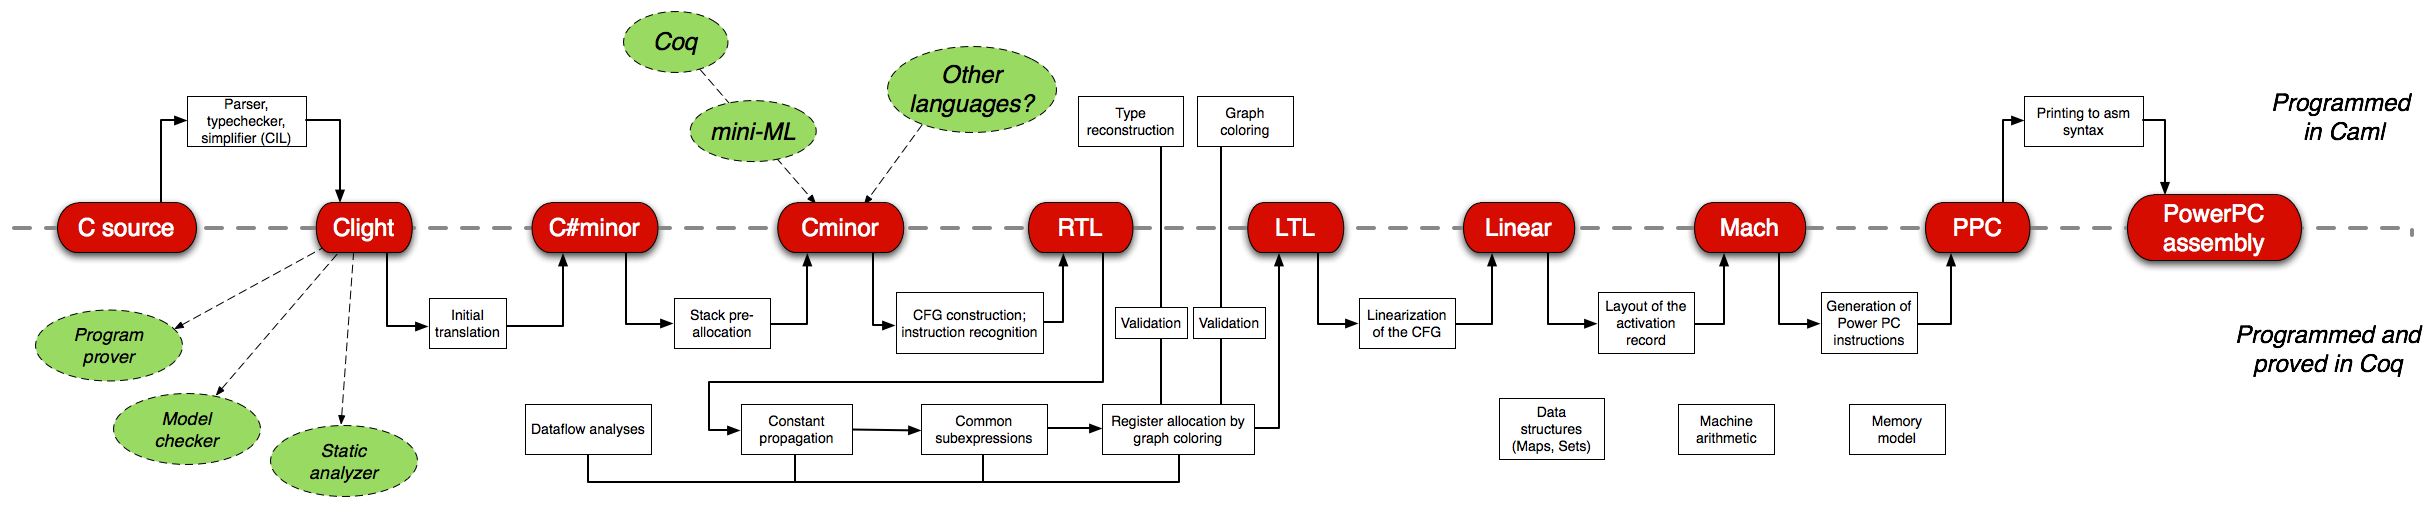
\includegraphics[width=\textwidth]{compcert-diagram.png}
\end{center}
\caption{Organization of CompCert (from~\cite{compcert-web})  \jeehoon{too old, change it}}
\label{fig:compcert-organization}
\end{figure}

To verify compilation correctness for the compiler $\mathcal{C}$, we verify each pass of
$\mathcal{C}$ independently.  Specifically, for each pass (transformation) $\mathcal{T}$ from
language $L_1$ to $L_2$---where the $L_i$'s may be C, assembly, or some intermediate languages---we
show the following:
\[
\frac{
\mathcal{T}(\mathtt{s.l1}) = \mathtt{t.l2} \qquad
s = \mathrm{load}(\mathtt{s.l1}) \qquad
t = \mathrm{load}(\mathtt{t.l2})
}
{
\mathrm{Behav}(s) \supseteq \mathrm{Behav}(t)
}
\]
That is, given the input \code{s.l1} and output \code{t.l2} of the $\mathcal{T}$ transformation, we
show that the behaviors of \code{t.l2} are contained within those of \code{s.l1}.  Since subset
inclusion is transitive, it easy to see that the proofs of the constituent passes of $\mathcal{C}$
compose to establish the correctness of $\mathcal{C}$ as a whole.

It is worth noting that CompCert consists of around a dozen optimization and transformation passes
going through quite a few intermediate languages, as illustrated in
\Cref{fig:compcert-organization}, and mainstream compilers typically have dozens of passes.


\paragraph{Verifying Per-Pass Correctness}

Now how does one actually prove the verification condition for each individual pass?  The standard
approach taken by CompCert is to use (closed) simulations.  Informally, we will say that a
\emph{simulation} $R$ is a relation between running programs (\ie machine states) in $L_1$ and $L_2$
such that, if $(s,t) \in R$, then the behaviors one observes while stepping through the execution of
$t$ are matched by corresponding observable behaviors in the execution of $s$.  One can think of $R$
as imposing an invariant, which describes (and connects) the possible machine states of the source
and target programs, and which must be maintained as the programs execute.  We leave further details
about simulations until later in the paper; suffice it to say that they satisfy the following
``adequacy'' property:
% , and we show that the machine states arising from
% loading \code{s.l1} and \code{t.l2} belong to this simulation.
\[
\frac{
R~\mbox{is a simulation} \qquad
(s,t)\in R
}{
\mathrm{Behav}(s) \supseteq \mathrm{Behav}(t)
}
\]
Thus, to establish the verification condition for pass $\mathcal{T}$, it suffices to exhibit a
simulation $R$ that relates $\mathrm{load}(\mathtt{s.l1})$ and $\mathrm{load}(\mathtt{t.l2})$.

\textbf{Note:} The verification approach described above, relying on ``backward'' simulations, is
something of an oversimplification of what CompCert actually does.  In fact, to make the proofs more
convenient, CompCert uses a mixture of forward and backward simulations.  We gloss over this point
here because it is orthogonal to our story, but we will return to it in \Cref{chap:sepcomp}.




\subsection{The RTL Language}
\label{sec:background:rtl}

\jeehoon{Revised up here}


In the rest of this section, we will explain how to establish a simulation relation for optimization
passes, using constant propagation as a running example.  We start with the syntax and semantics of
CompCert's register transfer language (RTL), the compiler's internal language where constant
propagation takes place.  For presentation purposes, we simplify the language a bit by removing
types and other unnecessary details.


\paragraph{Syntax}

% \begin{figure}
\[
\begin{array}{@{}l@{~}c@{~}l@{~~}lr@{}}
\rtlProg &::=& \overline{\rtlDecl}
\\
\rtlDecl &::=& 
\multicolumn{2}{@{}l@{}}{\rtlextern~\consthide{[\rtlconst]~}\typhide{\typhide{\mathit{Typ}~}}\rtlId[Int]} &\text{// External Variable} \\
&|&\multicolumn{2}{@{}l@{}}{\consthide{[\rtlconst]~}\typhide{\mathit{Typ}~}\rtlId[Int] := \{~\overline{\rtlGVal}~\}} & \text{// Variable}\\
&|&\multicolumn{2}{@{}l@{}}{\rtlextern~\typhide{\mathit{Typ}~}\rtlId~\rtlFSig} & \text{// External Function}\\
&|&\multicolumn{2}{@{}l@{}}{\typhide{\mathit{Typ}~}\rtlId~\rtlFunc} & \text{// Function}
\\
\rtlFSig &::=& 
\multicolumn{2}{@{}l@{}}{(\overline{\typhide{\mathit{Typ}~}\rtlReg})}
&\text{// Function Signature}
\\
\rtlFunc &::=& 
\multicolumn{2}{@{}l@{}}{(\overline{\typhide{\mathit{Typ}~}\rtlReg})~
\setof{\overline{\typhide{\mathit{Typ}~}\rtlReg};~\rtlsp[\rtlInt]~;~\rtlCode}}
&\text{// Function Definition}
\\
\typhide{\mathit{Typ} &::=& \mathtt{int}~|~\mathtt{float}~|~\ldots\\}
\rtlCode &::=& \overline{\rtlNId:\rtlInstr}\\
\end{array}
\]
\vspace{-2ex}
\[
\begin{array}{@{}l@{~}c@{~}l@{~~}l@{}r@{}}
\rtlInstr &::=& \rtlReg := \rtlFVal&\rtljmp~\rtlNId&\text{// Immediate Value}
\\&|&\rtlReg := \rtlop~\overline{\rtlReg}&\rtljmp~\rtlNId&\text{// Operation}
\\&|&\rtlReg :=\rtlFVal[Int]&\rtljmp~\rtlNId&\text{// Load}
\\&|&\rtlFVal[Int] :=\rtlReg&\rtljmp~\rtlNId&\text{// Store}
\\&|&\multicolumn{2}{@{}l@{}}{\rtlcondop~\overline{\rtlReg}~?~\rtljmp~\rtlNId:\rtljmp~\rtlNId}&\text{// Conditional}
\\&|& \rtlReg := \rtlFVal(\overline{\rtlReg})&\rtljmp~\rtlNId&\text{// Call}
\\&|&\multicolumn{2}{@{}l@{}}{\rtlreturn~\rtlReg} &\text{// Return}
\\&|&\ldots\\
\end{array}
\]
\vspace{-1ex}
\[
\begin{array}{@{}l@{~}c@{~}l@{~~}lr@{}}
\rtlGVal&::=&\multicolumn{2}{@{}l@{}}{\rtlId ~|~ \rtlInt ~|~ \rtlundef}\\
\rtlFVal&::=&\multicolumn{2}{@{}l@{}}{\rtlGVal ~|~ \rtlReg ~|~ \rtlsp}\\
\rtlInt&::=&\multicolumn{2}{@{}l@{}}{\text{the set of 32-bit integers}}\\
\rtlId&::=&\multicolumn{2}{@{}l@{}}{\text{the set of identifiers for variables and functions \qquad\qquad\qquad}}\\
\rtlReg&::=&\multicolumn{2}{@{}l@{}}{\text{the set of register names}}\\
\rtlNId&::=&\multicolumn{2}{@{}l@{}}{\text{the set of node labels}}\\
\end{array}
\]
\caption{RTL syntax}
\label{fig:rtl-syntax}
\end{figure}


%%% Local Variables:
%%% mode: latex
%%% TeX-master: "main"
%%% TeX-command-extra-options: "-shell-escape"
%%% End:

% TODO

The syntax of the CompCert's RTL is given in Figure~\ref{fig:rtl-syntax}.  Programs are just a list
of global declarations, which consist of $(1)$ declarations of external variables and functions
provided by different compilation units, and $(2)$ definitions of variables and functions provided
by the current compilation unit.  For global variable declarations and definitions, we also specify
a (positive) integer number denoting the size of the declared block in bytes.

Function declarations only contain the function signature, which is a list of parameters, but
function definitions additionally contain a list of local registers, the size of their stack frame,
and the code.  The code is essentially a control-flow graph of three-address code: it is represented
as a mapping from node identifiers to instructions, where instructions either
%
do some local computation (\eg write a constant to a register, or perform some arithmetic
computation),
%
load from a memory address, 
%
store to memory,
%
do a comparison,
%
call a function, 
%
or exit the function and return a result. 
%
Each instruction also stores the node identifier(s) of its successor instruction(s).

Throughout we assume that programs satisfy some basic well-formedness properties: there cannot be
multiple definitions for the same global variable, declarations and definitions of the same variable
should have matching signatures, and the parameter and local variable lists for each function do not
have duplicate entries.


\paragraph{Semantics}

\jeehoon{defer memory model to the next subsection.}

% %!TEX root=main.tex

\begin{figure}
\[\begin{array}{@{}l@{~}c@{~}l@{}}
\rtlMem &\defeq& \setof{(nb,bs)\suchthat nb\in\rtlBId\land bs \in \rtlBId \fpfun \rtlBlock} \\
\rtlBlock &\defeq&
\setof{(p, n, c) \suchthat
  p \in \setofz{\rtlvalid,\rtlfreed} \land n \in \Nat \land c \in \rtlVal^n \!} \\
\rtlVal &\defeq& \rtlInt \uplus \rtlAddr \uplus \setofz{\rtlundef} \\
\rtlAddr &\defeq& \setof{(l,i) \in \rtlBId\times \rtlInt} \\
\rtlGEnv &\defeq& \setof{(g,d)\suchthat g\in \rtlId \fpfun \rtlBId {}\land{}\\
&&\qquad\quad~~~ d \in \rtlBId \fpfun \rtlFSig\uplus\rtlFunc}\\
\rtlState &\defeq& \rtlIState\uplus\rtlCState\uplus\rtlRState\\
\rtlIState&\defeq& \setof{\rtlist~m~s~\vfd~sp~pc~rs \suchthat\\
&&~~
m\in\rtlMem\land s\in\overline{\rtlStkFrm}
\land\vfd\in\rtlFunc\land{}\\
&&~~sp\in\rtlAddr \land pc\in\rtlNId\land
rs\in \rtlReg \fpfun \rtlVal
}
\\
\rtlCState&\defeq& \setof{\rtlcst~m~s~\vfds~vs\suchthat
m\in\rtlMem\land s\in\overline{\rtlStkFrm}{}\land{}\\
&&~~\vfds\in\rtlFunc\uplus\rtlFSig\land vs\in\overline{\rtlVal}
}
\\
\rtlRState&\defeq& \setof{\rtlrst~m~s~v \suchthat
m\in\rtlMem\land s\in\overline{\rtlStkFrm}\land
v\in \rtlVal
}
\\
\rtlStkFrm &\defeq& \setof{(r,\vfd,sp,pc,rs)\suchthat
r\in\rtlReg\land \vfd\in\rtlFunc\land{}\\
&&~~ sp\in\rtlAddr \land pc\in\rtlNId\land
rs\in \rtlReg \fpfun \rtlVal
}
\end{array}
\]
\caption{RTL semantic domains}
\label{fig:rtl-semdom}
\end{figure}

%%% Local Variables: 
%%% mode: latex
%%% TeX-master: "main"
%%% TeX-PDF-mode: t
%%% End: 

% TODO

We move on to the semantics of RTL.  Figure~\ref{fig:rtl-semdom} defines the necessary semantic
domains.

Memory, $m\in\rtlMem$, is represented as a finite collection of allocation blocks (a mapping from
block identifiers to blocks), each of which is a contiguous portion of memory that may be either
valid to access or already deallocated (freed) and therefore invalid to access.  CompCert values,
$v\in\rtlVal$, can be either 32-bit integers, logical addresses (pairs of a block identifier
together with an offset within the block), or the special $\rtlundef$ value used to represent
uninitialized data.  A global environment, $ge=(g,d)\in\rtlGEnv$, maps each global variable name to
a logical block identifier, and each logical block identifier corresponding to some function's code
to either the corresponding function signature for external functions or the corresponding function
definition for functions defined in the program.

Next, program states can be of three kinds: normal instruction states ($\rtlist$), call states
($\rtlcst$) just before passing control to an invoked function, and return states ($\rtlrst$), just
after returning from an invoked function.  Instruction states store the memory ($m$), the sequence
of parent stack frames ($s$), the definition of the function whose body is currently executed
($\vfd$), the current stack pointer ($sp$), the program counter ($pc$), and the contents of the
local registers ($rs$).  Call states record the memory, the stack, and the function to be called
($\vfds$) with its arguments ($args$).  The function to be called can be either an internal
function, in which case we record its definition, or an external one, in which case we record its
signature.  Return states record just the memory, the stack, and the value that was returned by the
function.  A stack $s$ is a list of stack frames, each of which records the same information as
normal instruction states, except with the addition of a register name $r$ where its return value
should be stored, and minus the memory ($m$) and stack ($s$) components.

The meaning of programs is described by three definitions:
\[
\begin{array}{r@{~~}c@{~~}l}
\rtlgenv &\in& \rtlProg \to \rtlGEnv \\
\rtlload &\in& \rtlProg \pfun \rtlState\\
\estep{} &\in& \powset{\rtlGEnv\times\rtlState\times\rtlEvent\times\rtlState}\\
\end{array}
\]
The first function, $\rtlgenv(\vprg)$, returns the global environment corresponding to the program:
it `allocates' the global variables of the program sequentially in blocks 1, 2, 3, and so on, and
maps the blocks corresponding to function symbols to the relevant function definition or signature.

Similarly, $\rtlload(\vprg)$ returns the initial state obtained by loading a program into memory: it
initializes the memory $m$ with the initial values of the global variables at the appropriate
addresses generated by $\rtlgenv(\vprg)$, and returns a call state, $\rtlcst~m~[\,]~\vfd~[\,]$,
where $\vfd$ is the function definition corresponding to \texttt{main()}.  Loading is a partial
function because it is undefined for programs without a \texttt{main()} function.

% \begin{figure*}[!]
\footnotesize
\begin{mathpar}
\inferrule[(imm)]{
\begin{array}{c}
\vfd @  pc = (dst := src~\rtljmp~pc')\\
rs' = rs[dst\leftarrow \sem{src}(ge,sp,rs)]\\
\end{array}
}{
\rtlist~m~s~\vfd~sp~pc~rs
\estep{\epsilon}_{ge}
\rtlist~m~s~\vfd~sp~pc'~rs'
}

\inferrule[(op)]{
\begin{array}{c}
\vfd @  pc = (dst := \rtlop~\vargs~\rtljmp~pc')\\
rs' = rs[dst\leftarrow \sem{\rtlop}(ge,sp,\sem{\vargs}(rs))]\\
\end{array}
}{
\rtlist~m~s~\vfd~sp~pc~rs
\estep{\epsilon}_{ge}
\rtlist~m~s~\vfd~sp~pc'~rs'
}

\inferrule[(load)]{
\begin{array}{c}
\vfd @ pc = (dst := src[n]~\rtljmp~pc')\\
(l,i) = \sem{src}(ge,sp,rs)\\
rs' = rs[dst\leftarrow m[(l,i+n)]]\\
\end{array}
}{
\rtlist~m~s~\vfd~sp~pc~rs
\estep{\epsilon}_{ge}
\rtlist~m~s~\vfd~sp~pc'~rs'
}

\inferrule[(store)]{
\begin{array}{c}
\vfd @ pc = (dst[n] := src~\rtljmp~pc')\\
(l,i) = \sem{dst}(ge,sp,rs)\\
m' = m[(l,i+n)\leftarrow \sem{src}(rs)]\\
\end{array}
}{
\rtlist~m~s~\vfd~sp~pc~rs
\estep{\epsilon}_{ge}
\rtlist~m'~s~\vfd~sp~pc'~rs
}

\inferrule[(cond)]{
\begin{array}{c}
\vfd @  pc = 
(\rtlcondop~\vargs~?~\rtljmp~pc_1:\rtljmp~pc_2)\\
b = \sem{\rtlcondop}(ge,sp,\sem{\vargs}(rs)) \\
pc' = b ~?~ pc_1 : pc_2\\
\end{array}
}{
\rtlist~m~s~\vfd~sp~pc~rs
\estep{\epsilon}_{ge}
\rtlist~m~s~\vfd~sp~pc'~rs
}

\inferrule[(call1)]{
\begin{array}{c}
\vfd @ pc = (res := f(\vargs)~\rtljmp~pc')\\
(l,0) = \sem{f}(ge,sp,rs) \\
\vfds' = \mathrm{findfunc}(ge,l) \\
vs = \sem{\vargs}(rs) \\
\end{array}
}{
\rtlist~m~s~\vfd~sp~pc~rs
\estep{\epsilon}_{ge}
\rtlcst~m~((res,\vfd,sp,pc',rs){::}s)~\vfds'~vs
}

\inferrule[(call2-internal)]{
\begin{array}{c}
(m',l) = \mathrm{alloc}(m, \mathrm{stacksize}(\vfd))\\
pc = \mathrm{entrynode}(\vfd)\\
rs = \mathrm{init\text{-}regs}(\mathrm{params}(\vfd),vs)\\
\end{array}
}{
\rtlcst~m~s~\vfd~vs
\estep{\epsilon}_{ge}
\rtlist~m'~s~\vfd~(l,0)~pc~rs
}

\inferrule[(call2-external)]{
\begin{array}{c}
(\vevt,v,m') \in \mathrm{extcall\text{-}sem}(\vfs,ge,vs,m) \\
\end{array}
}{
\rtlcst~m~s~\vfs~vs
\estep{\vevt}_{ge}
\rtlrst~m'~s~v
}

\inferrule[(return1)]{
\begin{array}{c}
\vfd @ pc = (\rtlreturn~r)\\
v = \sem{r}(rs) \\
m' = \mathrm{free}(m,sp,\mathrm{stacksize}(\vfd)) \\
\end{array}
}{
\rtlist~m~s~\vfd~sp~pc~rs
\estep{\epsilon}_{ge}
\rtlrst~m'~s~v
}

\inferrule[(return2)]{
rs' = rs[res \leftarrow v]
}{
\rtlrst~m~(res,\vfd,sp,pc,rs){::}s~v
\estep{\epsilon}_{ge}
\rtlist~m~s~\vfd~sp~pc~rs'
}

\end{mathpar}
\caption{Operational semantics of RTL}
\label{fig:rtl-opsem}
\end{figure*}



%%% Local Variables:
%%% mode: latex
%%% TeX-master: "main"
%%% TeX-command-extra-options: "-shell-escape"
%%% End:

% TODO

The $\estep{}$ relation is a small-step reduction relation describing how program states evolve
during the computation.  For clarity, we write $s \estep{\vevt}_{ge} s'$ instead of
$(ge,s,\vevt,s')\in {\estep{}}$.  The operational semantics for RTL is fairly standard and shown in
Figure~\ref{fig:rtl-opsem}: there is a rule for each of the various basic instructions of the
language.  Starting from normal instruction states, the instruction at the node pointed to by the
program counter is scrutinized ($\vfd@pc$).  Depending on what instruction is there, only one rule
is applicable.  The corresponding rule calculates the new values of the registers, the memory (for
store instructions), and the next program counter.  Calls and returns are treated a bit differently:
they do not directly transition from an instruction state to the next instruction state---they go
through an intermediate call/return state.

In more detail, calling a function (rule \textsc{call}) looks up the function in the global
environment, evaluates its arguments, creates a new stack frame corresponding to the current
instruction state, and transitions to a call state.  From a call state, there are two possible
execution steps.  If the function to be called is internal, \ie we have its function definition
$\vfd\in\rtlFunc$, rule \textsc{internal-call} applies.  It allocates the necessary stack space for
the called function, initializes the parameter registers with the values passed as arguments, sets
the program counter to point to the first node of the called function, and moves to the appropriate
instruction state of the called function.  If the function to be called is external, \ie we have a
function signature $\vfs\in\rtlFSig$, rule \textsc{external-call} goes directly to the return state,
and generates an event $\vevt$ indicating that it called an external function.

Conversely, returning from a function (rule \textsc{return}) evaluates the result to be returned,
deallocates the stack space used by the function, and transitions to the return state.  The only
possible step form a return state (rule \textsc{return2}) then pops the top-most stack frame and
transitions to a normal instruction state thereby restoring the registers, program counter, and
stack pointers of the calling function.



\subsection{The Memory Model}
\label{sec:background:memory}

To simplify the presentation, we focus on handling integer-pointer casts and relaxed-memory
concurrency and do not discuss many of the orthogonal aspects of C semantics.  Specifically, we
$(1)$ assume a 32-bit architecture: words are 4 bytes wide, and the size of the address space is
$2^{32}$, $(2)$ consider only integer and pointer values, and omit values of other types such as
\texttt{float} or \texttt{char}, and $(3)$ omit subword arithmetic, and assume each address stores a
32-bit value.  \jeehoon{check it.}
% and take all addressing to be aligned at 4-byte boundaries.  \todo{gil: this is not quite
% right. For example, we have a 4-byte word at 0x0000FFF0 and another 4-byte word at 0x0000FFF1,
% ratherthan at 0x0000FFF4.  We used this just for simplicity anyway.}  $(l,i)$ points to the $i$-th
% cell of 4 byte data in the logical block $l$).


\paragraph{Concrete Model}

Concrete memory consists of a $2^{32}$-sized array of values, and a
list of allocated blocks, 
represented as pairs $(p,n)$ of the block's starting address and its size.
Loading from or storing to an unallocated address raises
an error (\ie undefined behavior).  Values are just 32-bit integers,
since pointers are merely integers in the concrete model.
As a result, \emph{the concrete model natively supports integer-pointer casts}.
\[
\begin{array}{@{}l@{~}c@{~}l@{}}
\mathrm{Mem} &\defeq& (\inttype \to \mathrm{Val}) \times \mathtt{list}\ \mathrm{Alloc} \\
\mathrm{Alloc} &\defeq& \setof{(p,n) \suchthat p \in \inttype \land n \in \inttype} \\
\mathrm{Val} &\defeq& \setof{i\in\inttype}
\end{array}
\]

Memory allocation inserts a block into the list of allocated blocks, 
whereas deallocation removes one.  Overall, the list of allocated 
blocks should be \emph{consistent}:\footnote{These are a subset of 
  \texttt{malloc}'s properties according to the C11 Standard~\cite{iso2011iec}. 
  For more details, see \S7.22.3 paragraph~1 and \S6.5.8 paragraph~5.}
\begin{itemize}
\item If $(p, n)$ is allocated, then $\emptyset \neq [p,p+n) \subseteq
  (0,2^{32}-1)$.
%\item If $(p, n)$ is allocated, then $p\neq 0$ and $n\neq 0$.
\item If blocks $(p_1, n_1)$ and $(p_2, n_2)$ are distinct
  allocations, their ranges $[p_1,p_1+n_1)$ and $[p_2,p_2+n_2)$
  are disjoint.
\end{itemize}

As we have seen, however, the concrete model \emph{does not support 
standard compiler optimizations} such as constant propagation and 
dead allocation elimination in the presence of external function
calls.  This is because the model does not provide 
a mechanism for ensuring that a module has exclusive control over some
part of memory, thereby assuming that unknown code can read and 
update the contents of every allocated memory cell.


\paragraph{CompCert's Logical Model}

In CompCert's logical model
\cite{leroy:compcert,Leroy-Appel-Blazy-Stewart-memory-v2}, memory
consists of a finite set of logical blocks with unique block
identifiers.  Each block is a fixed-sized array of values together
with a validity flag $v$ that indicates whether the block is accessible or
has been freed. As before, accessing a freed block raises an error.
Values are either 32-bit integers or logical addresses.  Here, a
logical address $(l,i)$ consists of a block identifier $l$ and an
offset $i$ inside the block.
% (For simplicity, throughout this paper, we assume pointers
%are aligned at 4-byte boundaries and $(l,i)$ represents the 4-byte chunk at
%offset $4i$. \todo{This is not right for the same reason as before.})
%For a block identifier $l$, we henceforth write the 
%block $l$ for the block with identifier $l$.
\[
\begin{array}{@{}l@{~}c@{~}l@{}}
\mathrm{Mem} &\defeq& \mathrm{BlockID} \fpfun \mathrm{Block} \\
\mathrm{Block} &\defeq&
\setof{(v, n, c) \suchthat
  v \in \mathtt{bool} \land n \in \Nat \land c \in \mathrm{Val}^n } \\
\mathrm{Val} &\defeq& \setof{i\in\mathtt{int32}} \uplus \setof{(l,i) \in \mathrm{BlockID}\times \mathtt{int32}}
\end{array}
\]

An important advantage of the logical model over the concrete one is that 
it \emph{allows functions to have exclusive control over a logical block} as 
long as they do not allow its address to escape. The reason is that it
is not possible to manufacture the logical address of an already allocated block.  
This property guarantees the correctness of many useful optimizations, 
such as constant propagation across function calls and dead allocation
elimination.

A secondary advantage is that programs have \emph{infinite memory}, rendering
their allocation behavior unobservable, which in turn makes it easy for
compilers to remove dead allocations.

%% there is no out-of-meory behavior since the memory has infinitely many logical blocks.
%This is important because even if a source program consumes a huge
%amount of memory, ... (\todo{Viktor, please say something about this
% :)})

Apart from that logical models have a slightly more complicated
semantics, their main disadvantage is that \emph{they do not support
  integer-to-pointer casts} very well.
%% The main disadvantages of logical models are that they have a slightly
%% more complicated semantics and, most importantly, that \emph{they do
%%   not support integer-to-pointer casts} very well.  
As a result,
CompCert has very weak support for integer-pointer casts.  Generally,
they are treated as \texttt{nop}s (\ie the identity function) rather
than undefined (\ie erroneous), and thus variables of integer (or
pointer) types can contain both integers and logical addresses.  In
CompCert's higher-level languages (CompCert C and Clight), once a
pointer is cast into an integer, any arithmetic on that integer
returns an unspecified value.  In its lower-level languages (Cminor,
RTL, \emph{etc.}), however, some of the integer operations (namely,
addition, subtraction, and equality tests) are also well-defined for
pointer values in special cases.  More specifically, for instance,
%% subtraction and equality test are well defined for pointer values in
%special cases: \eg 
the addition of an integer to an address, the
subtraction between addresses when they are in the same logical block,
and the equality test between an address and \texttt{NULL} are well-defined.



\subsection{Constant Propagation}
\label{sec:background:constprop}

\paragraph{Algorithm}

Given a program $\vprg$, constant propagation walks through each function definition $\vfd$ of the program 
and transforms it using the function $\mathrm{transfun}(\vprg, \vfd)$.
This in turn runs a ``value analysis'' to determine which variables (whether global variables or local registers) hold a known constant value at each program point
and then, based on that information, simplifies the program.

The analysis consists of two parts: 
(a) the global part, which detects which global variables cannot be updated (\ie those declared with the \texttt{const} qualifier), and
(b) the local part, which analyzes the code of a function and calculates an abstract value for each register and stack variable.
The abstract value of a variable can be either $\bot$ if the variable holds $\tt undef$, 
or a constant number, 
or $\NSmac$ if the variable contains anything except for a pointer pointing into the current stack frame, 
or $\top$ if no more precise information is known.
These abstract values form a lattice by taking the order $\bot \sqsubseteq \mathit{num} \sqsubseteq \NSmac \sqsubseteq \top$.


The value analysis performs a usual traversal of the code. 
When calling a function, 
if it can be determined that no memory address can point to the current stack frame 
and none of the function's arguments point to the current stack frame (\ie their abstract value is at most $\NSmac$), 
then the abstract value of the function's result is also $\NSmac$, and the abstraction of the stack memory is preserved.
If, however, a pointer to the current stack frame has escaped, then any information about the stack memory is forgotten.

The transformation part itself is straightforward: 
at each node $n$ of the function's CFG, if the analysis has determined that a variable has a constant value at node $n$,
then the use of that variable is replaced by the constant it holds, and the instruction is suitably simplified.

As an example, 
Figure~\ref{fig:const-prop-example} shows the effect of constant propagation applied to a simple program.
The program contains one internal function, \texttt{f}, which calls an external function, \texttt{g},
and three zero-initialized variables: 
a local variable (a register), \texttt{x}, 
an address-taken variable on the stack, \texttt{sp[0]},
and a global variable, \texttt{gv[0]}.
After the external function call, 
constant propagation can safely assume that $\texttt{x}=0$ and thereby simplify the conditional at node 5,
but cannot do the same for \texttt{sp[0]} at node 4
because its address was passed to the external function and its value might therefore have changed.
Further, at node 6, 
constant propagation notes that the global variable \texttt{gv[0]} has been declared with the \texttt{const} qualifier,
and can therefore assume that $\texttt{gv[0]}=0$.


% \input{constprop-example}
% TODO

\jeehoon{explain the examples in the intro.}



\paragraph{Verification}

The correctness proof of the constant propagation pass in CompCert establishes 
the existence of a simulation relation, $R$, that relates the loading of the source and target programs.
That is, for every well-formed source RTL program $\vprg$, it proves 
there exists a simulation $R(\vprg)$ such that 
$(\mathrm{load}(\vprg),\mathrm{load}(\mathcal{T}_\mathrm{cp}(\vprg)))\in R(\vprg)$.

The simulation relation, $R$, used for the constant propagation pass is given in
Figure~\ref{fig:part0-rel}.  It is defined in terms of matching relations on states, stack frames,
and stacks and function definitions ($\simState$, $\simFrame$, $\simStack$, and $\simFun$
respectively).  These relations take as a parameter the source program, $\vprg$, which is used to
relate the function definitions of the source and target programs.\footnote{The version shown here
  is a slight simplification of the actual simulation used in the constant propagation pass.  It
  abstracts away some tedious details of the actual $\simFrame$ definition that are orthogonal to
  our story.  This is merely to streamline the presentation.}

We say that two function definitions are related in the program $\vprg$, written $\vfd \simFun \vfd'$, 
if the target function, $\vfd'$, is the result of applying constant propagation to the source function, $\vfd$.
Two stack frames are related by $\vprg \vdash \vsf\simFrame \vsf'$ if 
the function code in $\vsf'$ is the transformation of the function code of $\vsf$,
the stack pointer and program counters agree, and
the registers of $\vsf'$ hold equal or more defined values than those of $\vsf$.
Two stacks are related, $\vprg \vdash s\simStack s'$, if they have the same length and their stack frames are related elementwise.

% \input{part0-simrel}
% TODO

Two states are related, $\vprg \vdash s \simState s'$
if $(1)$ they are of the same kind, 
$(2)$ the memory of $s'$ is an extension of that of $s$, 
%\todo{jeehoon: do we need to explain lessdef and extends relations?}
$(3)$ their stacks are related by $\simStack$,
$(4)$ the respective function definitions are related by $\simFun$ (when applicable),
$(5)$ the stack pointer and program counter agree (when applicable), and
$(6)$ the registers/arguments/return value of $s$ is equal or less defined than that of $s'$. 

Finally, the two states are in the simulation relation $R$
if they are related by $\simState$ and 
the source state satisfies the value analysis invariant, $\soundstate(\vprg,s)$.
This invariant basically says that the (concrete) value of each variable in the state $s$ is included in the variable's abstract value computed by the analysis at the current program point.
The invariant depends on the program for two reasons:
$(1)$ so that it can calculate the global environment, $ge=\rtlgenv(\vprg)$, and
$(2)$ so that it can `run' the analysis on the program so as to be able to compare its results with the current state.


The basic soundness properties of the value analysis are
$(1)$ that the $\soundstate$ invariant holds for the initial state of a program, and
$(2)$ that it is preserved by execution steps.
Formally:
\[
\frac{s = \rtlload(\vprg)}{
  \soundstate(\vprg,s)
}
\quad~~
\frac{ 
\begin{array}{c}
  \soundstate(\vprg,s) \\[-4pt]
  ge = \rtlgenv(\vprg)  \qquad
  s \estep{t}_{ge} s' 
\end{array}
}{
  \soundstate(\vprg,s')
}
\]

The CompCert proof then establishes $(1)$ that
\[(\mathrm{load}(\vprg),\mathrm{load}(\mathcal{T}_\mathrm{cp}(\vprg)))\in
R\] and $(2)$ that $R$ is a simulation relation. As for $(1)$, the
initial states after loading satisfy $\simState$ by construction, and
the initial source state satisfies $\soundstate$ thanks to the
soundness of the value analysis above.

It remains to show that $R$ is indeed a simulation.  Specifically,
CompCert shows that it is a ``forward'' simulation, meaning that for
any related states $(s,t)\in R$, if the source state $s$ takes a step
to $s'$ with an event $\sigma$, the target $t$ also takes a step to
\emph{some} state $t'$ with the same event $\sigma$, such that $(s',t')
\in R$.  From $(s,t)\in R$, we know that we are executing the
instructions at the same $\vpc$. Thus by the definition of constant
propagation, the target instruction is either identical to the source
instruction or obtained by replacing a variable with a constant or
converting a conditional jump to an unconditional jump, depending on
the value analysis result.  Here, thanks to the soundness of the
current state w.r.t.\ the analysis result and the relation between the
two states specified by $\simState$, we can easily deduce that
executing the source and target instructions results in related
states.  Also, the soundness of the new source state $s'$ follows
from the soundness preservation property of the value analysis stated
above.

Finally, we briefly discuss why CompCert establishes a forward
rather than a backward simulation, even though the former implies that
the source's behaviors refine the target's, which seems the wrong way
around.  First, a forward simulation is easier to establish than a
backward one because a single instruction in the source may be
compiled down to several instructions in the target. Second, CompCert
composes forward simulations of all passes using the transitivity of
forward simulations, which is not hard to show. Then it converts the
composed forward simulation between C and assembly to a backward
simulation between them using some technical properties of C and
assembly (namely, that C is \emph{receptive} and assembly is
\emph{determinate}). Finally, from this backward simulation, one can
establish that the target's behaviors refine the source's.

\jeehoon{explain backward simulation here, and defer discussion on forward simulation to
  \Cref{chap:sepcomp}.}


% Example language from intptrcast
%
% For concreteness, we consider the following simple C-like language:
% \[
% \begin{array}{@{}l@{~}c@{~}l@{}}
% \mathit{Typ} &::=& \texttt{int}~|~\texttt{ptr}\\
% \mathit{Bop} &::=& \texttt{+}~|~\texttt{-}~|~\texttt{*}~|~\texttt{\&\&}~|~\texttt{=}\\
% \mathit{Exp} &::=& \mathit{Int}~|~\mathit{Var}~|~\mathit{Global}~|~\mathit{Exp}\ \mathit{Bop}\ \mathit{Exp}\\
% \mathit{RExp} &::=& \mathit{Exp}~|~\texttt{malloc}(\mathit{Exp})~|~\texttt{free}(\mathit{Exp})~|~\texttt{(}\mathit{Typ}\texttt{)}\ \mathit{Exp}\\&&|~\texttt{input()}~|~\texttt{output}(\mathit{Exp})\\
% \mathit{Instr} &::=& \mathit{Fid}(\mathit{Exp}, \ldots, \mathit{Exp});
% ~|~\mathit{Var}\ \texttt{=}\ \mathit{RExp}
% ~|~\mathit{Var}\ \texttt{=}\ \texttt{*}\mathit{Exp}
% \\&&|~\texttt{*}\mathit{Exp}\ \texttt{=}\ \mathit{Exp}
% ~|~\texttt{if}\ \texttt{(}\mathit{Exp}\texttt{)}\ \overline{\mathit{Instr}}\ \texttt{else}\ \overline{\mathit{Instr}}
% \\&&|~\texttt{while}~\texttt{(}\mathit{Exp}\texttt{)}\ \overline{\mathit{Instr}}\\
% \mathit{Decl} &::=& \mathit{Fid}(\mathit{Typ}\ \mathit{Var}, \ldots, \mathit{Typ}\ \mathit{Var})\\&&\texttt{\{}\texttt{var}~\overline{\mathit{Typ}\ \mathrm{Var}};\,\overline{\mathit{Instr}}\texttt{\}}
% \end{array}
% \]
% The \texttt{input} and \texttt{output} operations produce externally visible events; all other operations are intended to model the corresponding operations in C.
% By $\overline{T}$ we mean a list of $T$.
% For simplicity, we omit \texttt{return} instructions and instead return values via pointer-valued arguments to functions.

%Our language has two types of values, integers and pointers, where the latter is represented as a pair $(l, i)$ of block identifier and integer offset. As a convention, we will use $\texttt{a}, \texttt{b}, \texttt{c}...$ for integer variables and $\texttt{p}, \texttt{q}, \texttt{r}...$ for pointer variables. 



\paragraph*{}

\jeehoon{Transition.}  It is important to note that this approach of using forward simulations (when
convenient) carries over without modification when porting CompCert to Level A and B compositional
correctness, as we do in the next section.



%%% Local Variables:
%%% mode: latex
%%% TeX-master: "main"
%%% TeX-command-extra-options: "-shell-escape"
%%% End:



\chapter{Relaxed-Memory~Concurrency}
\label{chap:relaxed}

%!TEX root = main.tex
\section{Introduction}\label{sec:introduction}

\newcommand{\sevcik}{\v{S}ev\v{c}\'{\i}k}

What is the right semantics for concurrent shared-memory programs
written in higher-level languages?  For programmers, the simplest
answer would be a \emph{sequentially consistent (SC)} semantics, in
which all threads in a program share a single view of memory and
writes to memory take immediate global effect.
% Under an SC semantics, all threads in a program share a single global
% view of memory and witness writes to memory in the same order, which
% is consistent with the program order (the sequential order of writes
% within any one thread).
%

However, a naive SC semantics is costly to
implement.  % \ori{I
  % think it is better to start with the fact that no existing hardware
  % actually implements SC.  seems more convincing than compiler
  % optimizations}
First of all, commodity architectures (such as x86, Power, and ARM)
are not SC: they execute memory operations speculatively or out of
order, and they employ hierarchies of buffers to reduce memory
latency, with the effect that there is no globally consistent view of
memory shared by all threads.  To simulate SC semantics on these
architectures, one must therefore insert expensive fence instructions
to subvert the efforts of the hardware.  Secondly, a number of common
compiler optimizations---such as constant propagation---are rendered
unsound by a naive SC semantics because they effectively reorder
memory operations.
% Commodity
% architectures are not SC either: they execute memory operations out of
% order, so simulating SC behavior at the hardware level typically
% requires the insertion of expensive fence instructions to prevent
% reorderings.
% Thus, to provide SC semantics for all memory
% accesses would entail disabling many compiler optimizations and
% inserting expensive fence instructions throughout pSa naive SC model
% of memory is also costly to implement efficiently.  implementing such
% a semantics for all memory accesses would be costly: it would (1)
% preclude common compiler optimizations that merge or reorder memory
% operations, preserving SC semantics through compilation is costly.
% Compiler optimizations like constant propagation effectively merge or
% reorder memory operations, and commodity hardware executes
% instructions out of order, so to support SC semantics for all accesses
% would require one to disable common compiler optimizations and insert
% expensive fence instructions throughout compiled code.
Moreover, SC semantics is stronger (\ie more restrictive) than
necessary for many concurrent algorithms.

Hence, languages like C/C++ and Java have opted instead to provide
\emph{relaxed} (aka \emph{weak}) memory models~\cite{jmm,c++17},
which enable programmers to demand SC semantics when they need it, but
which also support a range of cheaper memory operations that trade off
strongly consistent and/or well-defined behavior for efficiency.

\subsection{Criteria for a Programming Language Memory Model}
\label{sec:criteria}

Unfortunately, despite many years of research, it has proven very
difficult to develop a memory model for concurrent programming
languages that adequately balances the conflicting desiderata of
programmers, compilers, and hardware.  In particular, we would like to
find a memory model that satisfies the following properties:
% In particular, some basic properties one expects of such a memory
% model are the following:
\vspace{-.5ex}
\begin{itemize}
\item The model should support \emph{high-level reasoning} principles
  that programmers and compiler analyses depend on.  At a bare
  minimum, it should validate simple invariant-based verification, and
  should provide some ``DRF'' guarantees~\cite{Adve:1990}, ensuring that
  programmers who employ sufficient synchronization need not understand
  the full complexities of relaxed-memory semantics.\\[-2.5ex]
\item The model should be \emph{implementable}, \ie it should validate
  common compiler optimizations, as well as standard compilation
  schemes to the major modern architectures.  To be implementable, it
  must justify many kinds of instruction reordering and merging.\\[-2.5ex]
\item The model should ideally \emph{avoid relying on undefined
    behavior} to define the semantics of racy programs.  This is a
  prerequisite for applicability to type-safe languages like Java, in
  which well-typed programs may contain data races but are
  nevertheless expected to have safe, well-defined semantics.
\end{itemize}
\vspace{-.5ex}
\mbox{}\indent Both C/C++ and Java fail to achieve some of these criteria.

In the case of Java, the memory model fails to validate a number of
common program transformations performed by real Java compilers, such
as redundant read-after-read elimination and ``roach motel''
reordering~\cite{sevcik:jmm}.  Although this problem has been known
for some time, a satisfactory solution has yet to be developed.

In the case of C/C++, the memory model relies crucially on undefined
behaviors to give semantics to racy programs.  Moreover, it permits
certain ``out-of-thin-air'' executions which violate basic
invariant-based reasoning (and DRF guarantees)~\cite{Boehm2014}.
%To illustrate the problem, let us give a concrete example.

% \begin{itemize}
% \item Our model supports a wide range of common compiler and hardware
%   reorderings (including read-write, give list here, etc.)
% \ori{should we give the list? maybe the first is enough}.  We
%   establish the validity of these reorderings using fairly
%   straightforward simulation arguments.

% \item Our model rules out ``bad'' OOTA behaviors, such as $a$
%   receiving $1$ in \ref{eq:LBdep}.  As a result, we are able to prove standard
%   (and some non-standard) ``DRF theorems''.  These theorems guarantee
%   that programmers need not understand the full complexities of our
%   relaxed-memory semantics if they adhere to a restricted programming
%   discipline (\eg only racing on SC accesses \ori{under Sc semantics?}). 
%   In addition, our model supports the basic reasoning principle of global non-relational
%   invariants.

% % \item Our model supports basic invariant-based reasoning for relaxed
% %   accesses by prohibiting ``bad'' out-of-thin-air executions that
% %   would violate such reasoning.  It \emph{does} permit some other
% %   out-of-thin-air-\emph{ish} executions, but only ones that do not
% %   break invariant-based reasoning and that are arguably desirable to
% %   allow in any case because the ARM model allows them. \gil{ARM together with common compiler optimizations}

% \item Our model is designed to serve as a foundation for both C/C++
%   and Java.  On the one hand, it supports a range of different memory
%   operations (\eg nonatomic, SC, release-acquire, relaxed, fences) in
%   the style of C++.\footnote{Say something about correspondence with
%     C++ here?}  On the other hand, we do not rely on undefined
%   behavior/values to account for data races---programs have a fully
%   defined semantics under our model, which is a prerequisite for
%   applicability to a type-safe language like Java.

% % \item Our model validates standard (and some non-standard) ``DRF
% %   theorems''.  These theorems ensure that programmers who use only a
% %   subset of the supported language features (\eg only SC and nonatomic
% %   accesses) need not understand the more complex aspects of the model
% %   related to features they do not use.  (Is that right? What do we
% %   want to say here?)

% % \item
% % Say something about liveness here?
% \end{itemize}

% \section{Introduction}\label{sec:introduction}

% What is the right semantics for concurrent shared-memory programs
% written in higher-level languages?  For programmers, the simplest
% answer would be a \emph{sequentially consistent (SC)} semantics, in
% which all threads in a program share a single view of memory and
% writes to memory take immediate global effect.
% % Under an SC semantics, all threads in a program share a single global
% % view of memory and witness writes to memory in the same order, which
% % is consistent with the program order (the sequential order of writes
% % within any one thread).  
% %
% However, a naive SC semantics is costly to
% implement.  % \ori{I
%   % think it is better to start with the fact that no existing hardware
%   % actually implements SC.  seems more convincing than compiler
%   % optimizations}
% First of all, commodity architectures (such as x86, Power, and ARM)
% are not SC: they execute memory operations speculatively or out of
% order, and they employ hierarchies of buffers to reduce memory
% latency, with the effect that there is no globally consistent view of
% memory shared by all threads.  To simulate SC semantics on these
% architectures, one must therefore insert expensive fence instructions
% to subvert the efforts of the hardware.  Secondly, a number of common
% compiler optimizations---such as constant propagation---are rendered
% unsound by a naive SC semantics because they effectively reorder
% memory operations.
% % Commodity
% % architectures are not SC either: they execute memory operations out of
% % order, so simulating SC behavior at the hardware level typically
% % requires the insertion of expensive fence instructions to prevent
% % reorderings.
% % Thus, to provide SC semantics for all memory
% % accesses would entail disabling many compiler optimizations and
% % inserting expensive fence instructions throughout pSa naive SC model
% % of memory is also costly to implement efficiently.  implementing such
% % a semantics for all memory accesses would be costly: it would (1)
% % preclude common compiler optimizations that merge or reorder memory
% % operations, preserving SC semantics through compilation is costly.
% % Compiler optimizations like constant propagation effectively merge or
% % reorder memory operations, and commodity hardware executes
% % instructions out of order, so to support SC semantics for all accesses
% % would require one to disable common compiler optimizations and insert
% % expensive fence instructions throughout compiled code.  
% Moreover, SC semantics is stronger (\ie more restrictive) than
% necessary for many concurrent algorithms.  Hence, languages like Java
% and C++ have opted instead to provide \emph{relaxed} (aka \emph{weak})
% memory models~\cite{jmm,cppstandard}.  These models make it possible to enforce
% SC semantics when programmers need it, but they also support a range
% of cheaper memory operations that trade off strongly consistent and/or
% well-defined behavior for efficiency.

\subsection{The ``Out of Thin Air'' Problem}
\label{sec:oota}

% Unfortunately, both the Java and C++ memory models suffer from serious
% flaws  (see also \cite{Batty:2015}).  In the case of
% Java, the memory model fails to justify \ori{validate?} a number of common program
% transformations performed by real Java compilers, such as redundant
% read-after-read elimination and ``roach motel''
% reordering~\cite{sevcik:jmm}.  In the case of C++, the memory model
% permits certain ``out-of-thin-air'' executions which violate basic
% reasoning principles that programmers and compiler analyses depend on~\cite{Boehm2014}.

% (Maybe something here about how the JMM
% effort has stalled?) 

%

% To understand why satisfying all these criteria is so hard, let us
% look at a concrete example.  
To illustrate the problem with C/C++, consider these two variants of the
classic ``load buffering'' litmus test (with two threads in parallel):
% Consider these two variants of the classic ``load buffering'' litmus
% test (with two threads running concurrently):
\begin{center}
\begin{minipage}{.46\columnwidth}
\begin{equation}\label{eq:LB}\tag{LB}
\inarrII{ a:=x; \\ y:=1; }{ x:=y; }\!\!\!
\end{equation}
\end{minipage}
\hfill
\begin{minipage}{.46\columnwidth}
\begin{equation}\label{eq:LBdep}\tag{LBd}
\inarrII{ a:=x; \\ y:=a; }{ x:=y; }
\end{equation}
\end{minipage}
\end{center}
Here, we assume that all variables are initially $0$, and that all
memory accesses are of the weakest consistency level, \ie they are
compiled down to plain loads and stores at the hardware level with no
additional synchronization (in C/C++ this is called ``relaxed'').  The
question is: should it be possible for these programs to assign $1$ to
$a$?  In the case of \ref{eq:LB}, the answer is yes: architectures
like Power and ARM may reorder the write of $y$ before the read of $x$
in the first thread (since these are accesses to distinct variables),
after which $a$ can be assigned $1$ by a standard interleaving
execution. In the case of \ref{eq:LBdep}, however, the answer
\emph{ought} to be no: all the operations simply copy one variable to
another and all are initially $0$, so if $a$ could receive $1$, it
would come ``out of thin air''.  No hardware reorderings or reasonable
compiler optimizations will produce this behavior.  If they did, it
would cause major problems: one would not be able to establish even
basic invariants (such as $x = y = 0$), and basic sanity results like
the aforementioned DRF theorems would cease to hold.  It is therefore
a serious problem that the formal memory model of C/C++ allows such
out-of-thin-air (OOTA) behavior.
% \footnote{Actually, the C++ model
%   disallows this behavior with a vague English side condition, but it
%   does not explain clearly what OOTA means~\cite{n3710}.}

Intuitively, the reason C/C++ allows OOTA behaviors is that it is not
clear how to distinguish them from acceptable behaviors.  The C/C++
model formalizes valid executions as graphs of memory access events
(think: partially-ordered traces) subject to a set of coherence
axioms, and the same coherent event graph that describes a valid
execution of \ref{eq:LB} in which $a$ receives $1$ also describes a valid
execution of \ref{eq:LBdep} in which $a$ receives $1$.

% Naively, one might hope to solve this problem by exploiting information
% about syntactic dependencies between instructions in the program.
% In particular, one might hope to prohibit the OOTA behavior in \ref{eq:LBdep}
% by observing that the write to $y$ has a data dependency on the previous
% instruction, so the reordered execution of \ref{eq:LB} should not be applicable
% to \ref{eq:LBdep}.  Indeed, 

Hardware memory models (\eg Power and ARM) handle this problem by
taking syntactic dependencies between instructions into account in
determining program semantics.  Under such models, the out-of-order
execution in \ref{eq:LB} is valid because the write to $y$ is independent of
the read from $x$, whereas in \ref{eq:LBdep} such out-of-order execution is
prevented by the syntactic dependency between the two instructions.
Although this approach is suitable for modeling hardware, it is too
brittle for a language-level semantics because it fails to validate
standard compiler optimizations that remove syntactic dependencies (see also \cite{Boehm2014}).
As a very simple example, consider the following variant of \ref{eq:LB} and
\ref{eq:LBdep}:
\begin{equation}\label{eq:LBfalsedep}\tag{LBfd}
\inarrII{ a:=x; \\ y:=a+1-a; }{ x:=y; }
\end{equation}
Under the hardware models, this \ref{eq:LBfalsedep} program would be treated
similarly to \ref{eq:LBdep} due to the syntactic data dependency, so $a$ could
not receive $1$.  But even a basic optimizing compiler could trivially
transform \ref{eq:LBfalsedep} to \ref{eq:LB}, in which case $a$ could receive $1$.
%\ori{a simple answer here is that one can bake in the compiler optimizations
%to the definition of dependency, should we explain why it is really not working?}
%\jeehoon{Ori, I think that is too much information in the introduction.  How about saying it in the result section?}

% A naive solution to this problem would be for the semantics to 
% loads and delay their execution to the point when their value is
% actually used.  Such a semantics would enable reordering in the case
% of \ref{eq:LB}, but would prevent the OOTA behavior in the case of \ref{eq:LBdep}
% because there is a syntactic dependency of $y := a$ on the previous
% instruction.  Indeed, this approach has been successfully applied in
% definitions of hardware memory models.  


%   so if one can assign $1$ to
% $a$, one can assign any value to $a$.  And, the C11 model allows
% precisely this.  Not only is this behavior unintuitive---it also means
% that one cannot establish even simple global invariants such as
% $x = y = 0$, and one cannot prove standard ``sanity'' theorems like
% the DRF property.



% it suffers from the so-called ``out-of-thin-air'' (OOTA)
% problem.  Roughly speaking, the OOTA problem is the problem of how to
% provide a model of relaxed memory accesses that is weak enough to
% account for the reorderings/optimizations that hardware and compilers
% may perform, yet also strong enough to support at least some very
% basic reasoning that compiler analyses and programmers depend on (\eg
% global invariants on single variables).

% , namely the so-called
% ``out-of-thin-air'' problem~\cite{??,??}.  Roughly speaking, the
% problem is how to provide a model of relaxed memory accesses that is
% weak enough to account for the reorderings/optimizations that hardware
% and compilers may perform, yet also strong enough to support at least
% some very basic reasoning that compiler analyses and programmers
% depend on (\eg global invariants on single variables).  The existing
% models are either too strong (disallowing common compiler
% optimizations) or too weak (permitting variables to receive arbitrary
% ``out-of-thin-air'' values that break even basic invariant-based
% reasoning). 
%


As a result, we still to this day lack a semantics for relaxed-memory
concurrency in C/C++ and Java that corresponds to how these languages
are implemented and that provides sufficient reasoning guarantees to
programmers and compiler-writers.  Several proposals have recently
been made for how to fix the C/C++ and Java memory models (some of which
are discussed in \Cref{sec:related}), but none have been proven to
validate the full range of standard optimizations/reorderings
performed by C/C++ and Java compilers and by commodity hardware like
Power and ARM.  Furthermore, for most of the existing proposals, it is
known that indeed they do \emph{not} validate some important
reorderings.

\subsection{A ``Promising'' Semantics for Relaxed Memory}
\label{sec:promising}

In this paper, we present what we believe is a very promising way
forward: the first relaxed memory model to support a broad spectrum
of features from the C/C++ concurrency model while also satisfying all
three criteria listed in \Cref{sec:criteria}.


% \begin{itemize}
% \item
% Accounts for a broad spectrum of features of the C++11 memory model.
% \item

% \end{itemize}


% \begin{itemize}
% \item
% accounts for nearly all the features of the C++11 memory model,
% \item
% provably validates a number of standard compiler
%   optimizations, as well as a wide range of memory access reorderings
%   that commodity hardware may perform,
% \item avoids bad
%   ``out-of-thin-air'' behaviors that break invariant-based reasoning
% and DRF guarantees, and
% \item defines the semantics of racy programs without relying on
%   undefined behaviors.
% \end{itemize}


% \begin{itemize}
% \item Our model supports a wide range of common compiler and hardware
%   reorderings (including read-write, give list here, etc.)
% \ori{should we give the list? maybe the first is enough}.  We
%   establish the validity of these reorderings using fairly
%   straightforward simulation arguments.

% \item Our model rules out ``bad'' OOTA behaviors, such as $a$
%   receiving $1$ in \ref{eq:LBdep}.  As a result, we are able to prove standard
%   (and some non-standard) ``DRF theorems''.  These theorems guarantee
%   that programmers need not understand the full complexities of our
%   relaxed-memory semantics if they adhere to a restricted programming
%   discipline (\eg only racing on SC accesses \ori{under Sc semantics?}). 
%   In addition, our model supports the basic reasoning principle of global non-relational
%   invariants.

% % \item Our model supports basic invariant-based reasoning for relaxed
% %   accesses by prohibiting ``bad'' out-of-thin-air executions that
% %   would violate such reasoning.  It \emph{does} permit some other
% %   out-of-thin-air-\emph{ish} executions, but only ones that do not
% %   break invariant-based reasoning and that are arguably desirable to
% %   allow in any case because the ARM model allows them. \gil{ARM together with common compiler optimizations}

% \item Our model is designed to serve as a foundation for both C/C++
%   and Java.  On the one hand, it supports a range of different memory
%   operations (\eg nonatomic, SC, release-acquire, relaxed, fences) in
%   the style of C++.\footnote{Say something about correspondence with
%     C++ here?}  On the other hand, we do not rely on undefined
%   behavior/values to account for data races---programs have a fully
%   defined semantics under our model, which is a prerequisite for
%   applicability to a type-safe language like Java.

% % \item Our model validates standard (and some non-standard) ``DRF
% %   theorems''.  These theorems ensure that programmers who use only a
% %   subset of the supported language features (\eg only SC and nonatomic
% %   accesses) need not understand the more complex aspects of the model
% %   related to features they do not use.  (Is that right? What do we
% %   want to say here?)

% % \item
% % Say something about liveness here?
% \end{itemize}


We achieve these ends through a combination of mechanisms (some
standard, some not), but the most important and novel idea for the
reader to take away from this paper is the notion of \emph{promises}.

Under our model, which is defined by an operational semantics, a thread $T$ may nondeterministically ``promise''
to write a value $v$ to a memory location $x$ at some point in the
future.  From the point of view of other threads, a promise is no
different from an ordinary write: once $T$ has promised to write $v$
to $x$, other threads can read from that write.  (In contrast, $T$
cannot read from its own promised write until $T$ has fulfilled the
promise: this is crucial to preserve basic sanity of the semantics.)
Intuitively, promises simulate the effect of read-write reorderings by
allowing write events to be visible to other threads before the point
at which they occur in the program order.

We must, however, ensure that promises do not introduce bad OOTA
behaviors.  Toward this end, we only allow $T$ to promise to write $v$
to $x$ if it is possible to \emph{thread-locally certify} that the
promise can be fulfilled in a finite number of steps.
That is, we must show that $T$
will be able to write $v$ to $x$ after some finite sequence of steps
of $T$'s execution (\ie with no help from other threads).  The
certification requirement guarantees absence of bad OOTA executions by
ensuring that $T$ can only promise to write a value $v$ to $x$ if $T$
could have written $v$ to $x$ anyway.

Returning to the examples from \Cref{sec:oota}, it is easy to see how
promises give us the desired semantics:
\begin{itemize}
\item In \ref{eq:LB}, the first thread can promise to write $1$ to $y$ (since
  it will indeed write $1$ to $y$ no matter what value is assigned to
  $a$), after which the second thread can read from that promise and
  write $1$ to $x$.  Subsequently, the first thread can execute
  normally, reading $1$ from $x$ and assigning it to $a$.
\item The execution of \ref{eq:LBfalsedep} may proceed in exactly the same way.  The
  fact that the write of $y$ depends syntactically on $a$ is
  irrelevant, because during certification of the promised write of $1$
  to $y$, the expression $a+1-a$ will always evaluate to $1$.
\item By contrast, the OOTA behavior will not be allowed for \ref{eq:LBdep}.
  In order for the first thread to promise to write $1$ to $y$, it
  would need to certify that it can write $1$ to $y$ 
%in some finite number of steps 
without promises.  But since all variables are
  initially $0$, this is not possible.
\end{itemize}

Our model supports all features of C/C++ concurrency except consume
reads and SC accesses.  Consume reads are widely considered a
premature aspect of the C18/C++17 standard and are currently implemented
the same as acquire reads in mainstream compilers.  In contrast, SC
accesses are a major feature of C/C++, and originally our model included
an account of SC accesses as well.  However, in the course of trying
to prove the correctness of compilation to Power,
% (\Cref{sec:compilation_POWER}),
we discovered that our semantics of SC
accesses was flawed, and this led us to discover a flaw in the C/C++11
standard as well!  (See \cite{rc11} for further details.)
Thus, a proper handling of SC accesses remains an open and important
problem for future work.


% \derek{I removed this paragraph.  It didn't seem to really add anything.}
% In this way, promises provide a solution to the OOTA problem that does
% not rely on tracking brittle syntactic dependencies.  Furthermore, as
% we will see, the thread-local nature of our promise certification greatly
% simplifies the formal development of our semantics and has enabled us
% to straightforwardly prove the validity of read-write reorderings that
% were out of reach for prior work~\cite{Jagadeesan2010}.

% it is possible for $t$ to thread-locally \emph{validate} that $t$
% itself will be able to write $v$ to $x$ through a sequence of steps of
% its own execution.  (Hence, the name ``promise'': a thread can only
% promise a write event will happen if it itself will be the one to
% carry it out.)  Once $t$ has promised to write $v$ to $x$, other
% threads can read from that write, but $t$ itself cannot.  The
% validation requirement guarantees absence of ``bad'' out-of-thin-air
% executions by ensuring that a thread can never promise to write a
% value $v$ to $x$ unless it is possible for the thread to write $v$ to
% $x$ without making any promises.

% Intuitively, promises simulate the effect of read-write reorderings by
% allowing write events to be visible to other threads before the point
% where they occur in the program order.  The validation requirement
% guarantees absence of ``bad'' out-of-thin-air executions by ensuring
% that a thread can never promise to write a value $v$ to $x$ unless it
% could have in fact written $v$ to $x$ in a promise-free execution.
% Furthermore, the \emph{thread-local} nature of our promise validation
% greatly simplifies the formal development of our semantics and has
% enabled us to straightforwardly prove the validity of read-write
% reorderings that were out of reach for prior work~\cite{esop10??}.

% XXX

% Under our semantics, a thread $t$ may nondeterministically ``promise''
% to write a value $v$ to a memory location $x$ at some point in the
% future, but only if it is possible for $t$ to thread-locally
% \emph{validate} that $t$ itself will be able to write $v$ to $x$
% through a sequence of steps of its own execution.  (Hence, the name
% ``promise'': a thread can only promise a write event will happen if it
% itself will be the one to carry it out.)  Once $t$ has promised to
% write $v$ to $x$, other threads can read from that write, but $t$
% itself cannot.

% Intuitively, promises simulate the effect of read-write reorderings by
% allowing write events to be visible to other threads before the point
% where they occur in the program order.  The validation requirement
% guarantees absence of ``bad'' out-of-thin-air executions by ensuring
% that a thread can never promise to write a value $v$ to $x$ unless it
% could have in fact written $v$ to $x$ in a promise-free execution.
% Furthermore, the \emph{thread-local} nature of our promise validation
% greatly simplifies the formal development of our semantics and has
% enabled us to straightforwardly prove the validity of read-write
% reorderings that were out of reach for prior work~\cite{esop10??}.









% C11, for instance, distinguishes between
% \emph{nonatomic} accesses (intended for normal data accesses) and
% \emph{atomic} accesses (intended to implement synchronization between
% threads).  The former can be compiled efficiently, and their semantics
% is SC, but their behavior is only safe and well-defined if the programmer
% can guarantee the absence of data races on them.  The latter are specifically
% intended for racy access, but are available at a range of consistency 

% memory accesses: the former may be compiled efficiently but
% their behavior is only defined\emph{release-acquire} accesses (useful
% for implementing message-passing between threads where the global
% synchronization of SC is overkill), \emph{relaxed} accesses (useful
% for racy accesses where order of execution is not important) and
% \emph{non-atomic} accesses (for ``normal'' variablesand \emph{fully
%   relaxed} accesses. but they also permit programmers to indicate when
% the strength of SC semantics is not needed


% \subsection{Overview of the Paper}
% \label{sec:overview}

In the rest of the paper, we will flesh out the idea of promises---as
well as the other elements of our model---in layers.  We begin in
\Cref{sec:relaxed} by presenting the details of our model restricted
to relaxed reads and writes.  In \Cref{sec:updates}, we extend this
base model further to support atomic updates (\ie read-modify-write
operations, like CAS).  Then, in \Cref{sec:full}, we scale the model
up to handle most features of the C/C++ memory model.  In
\Cref{sec:results}, we present our formal results---validating many
program transformations, compilation to x86-TSO, DRF
theorems, and an invariant-based logic---most of which are fully
mechanized in the Coq proof assistant (totalling about 37K lines of
Coq).  In \Cref{sec:related}, we compare with related work, and in
\Cref{sec:discussion}, we conclude with discussion of future work.


%%% Local Variables:
%%% mode: latex
%%% TeX-master: "main"
%%% TeX-command-extra-options: "-shell-escape"
%%% End:

\newcommand{\figrelaxed}{
\begin{figure*}[t]
\small
\begin{mathpar}
%
\vspace*{-1mm}
%
\inferrule[\textsc{(thread: silent)}]
{
\sigma \astep{\silentt} \sigma' 
}
{\tup{\tup{\sigma, \rlxcur, \lprom}, \mem} \astep{} \tup{\tup{\sigma', \rlxcur, \lprom}, \mem}}
\and
\inferrule[\textsc{(thread: read)}]
{
 \sigma \astep{\rlab(x,v)} \sigma' \\
\rlxmsg{x}{v}{t} \in \mem \\\\
\rlxcur(x) \leq t \\
\rlxcur'=\rlxcur[x\mapsto t]
}
{\tup{\tup{\sigma, \rlxcur, \lprom}, \mem} \astep{} \tup{\tup{\sigma', \rlxcur', \lprom}, \mem}}
\and
\inferrule[\textsc{(thread: write)}]
{
 \sigma \astep{\wlab(x,v)} \sigma' \\
\mem'=\mem \insertadd \rlxmsg{x}{v}{t} \\\\
\rlxcur(x) < t \\
\rlxcur'= \rlxcur[x\mapsto t]
}
{\tup{\tup{\sigma, \rlxcur, \lprom},\mem} \astep{} \tup{\tup{\sigma', \rlxcur', \lprom}, \mem'}}
%
\\\vspace*{-1mm}
%
\inferrule[\textsc{(thread: promise)}]
{
\mem' = \mem \insertadd m \\
\lprom' = \lprom \insertadd m 
}
{\tup{\tup{\sigma, \rlxcur, \lprom},\mem} \astep{} \tup{\tup{\sigma, \rlxcur, \lprom'},\mem'}}
\and
\inferrule[\textsc{(thread: fulfill)}]
{
 \sigma \astep{\wlab(x,v)} \sigma' \\
\rlxmsg{x}{v}{t} \in \lprom \\
\lprom'=\lprom\setminus \setofz{\rlxmsg{x}{v}{t}} \\\\
\rlxcur(x) < t \\
\rlxcur' = \rlxcur[x\mapsto t] 
}
{\tup{\tup{\sigma, \rlxcur, \lprom},\mem} \astep{} \tup{\tup{\sigma', \rlxcur', \lprom'}, \mem}}
\and
\inferrule[\textsc{(machine step)}]
{\tup{\gts(i),\mem} \astep{}^+ \tup{\lts',\mem'} \\\\
\tup{\lts',\mem'} \text{ is consistent}}
{\tup{\gts,\mem} \astep{} \tup{\gts[i\mapsto \lts'],\mem'}}
\end{mathpar}
\caption{Operational semantics for the simplified model handling only relaxed read and write accesses.}
\label{fig:relaxed-opsem}
\end{figure*}}

\section{Basic Model for Handling Relaxed Accesses}
\label{sec:relaxed}

In this section, we introduce the key ideas of our memory model, first
by example and then more formally.  At first we will only consider a
semantics for fully ``relaxed'' atomic read and write accesses (in the
sense of C/C++).  This is a natural starting point, since the OOTA
problem is fundamentally about how to give a reasonable semantics for
these relaxed accesses, and the key elements of our solution are
easiest to understand in this simpler setting.  We will see in
subsequent sections how to extend and generalize this base model to
account for a much richer variety of memory operations.

To illustrate our semantics, we will write small programs such as the
following:
\begin{equation}\label{eq:SB}\tag{SB}
\inarrII{x:=1;\\a:=y;\comment{0}}{y:=1;\\b:=x;\comment{0}}
\end{equation}
As a convention, we write $a$, $b$, $c$ for local variables
(registers) and $x$, $y$, $z$ for (distinct) shared memory locations,
and assume that all variables are initialized to $0$.  
We refer to thread $i$ as $T_i$.  Moreover, in order to
refer to a specific observation of the program, we annotate the
corresponding reads with the values expected to be read (\eg in the
above program, the comment notation indicates the observed result that
$a = b = 0$).

\subsection{Main Ideas}

\paragraph{High-Level Requirements: Reorderings and Coherence}

Relaxed read and write operations are intended to be compiled down
directly to plain loads and stores at the machine level, so one of the
main requirements of our semantics is that it be at least as
permissive as commodity hardware.  Toward this end, our semantics must
justify reordering of independent memory operations (\ie operations
that access distinct locations), since the more weakly consistent
architectures (like ARM) may potentially perform such reorderings.
There are four such classes of reorderings---write-read, write-write,
read-read, and read-write---and in \Cref{sec:results} we will prove formally
that our semantics justifies all of them.

On the other hand,
% to support fundamental high-level reasoning
% principles, 
it is also important that our semantics not be
unnecessarily weak.  In particular, all the existing 
implementations of C/C++, even for weaker architectures like Power and
ARM, guarantee at a bare minimum a property we call \emph{per-location
  coherence} (aka \emph{SC-per-location}).  Per-location coherence
says that, even though threads may observe writes to different
locations in different orders, they must observe writes to the
\emph{same} location in a single total order (called the
``modification order'' in C/C++ lingo).
%, and it must be consistent with the
%``program order'' (the order in which writes are issued within any
%single thread). \ori{last sentence seems too partial to me: I suggest to remove
 In addition to being supported by hardware,
per-location coherence is preserved by common compiler optimizations
as well.  Hence, we want our semantics of relaxed accesses to
guarantee it. (In \Cref{sec:plain} we will present an even weaker mode of accesses that
does not provide full per-location coherence.)

%\jeehoon{we do not mention merges; I think it is reasonable at this stage, but I just want to make a note here.}

% This cut-down language is sufficient to understand
% the core of our solution to the OOTA problem without , and it is enough to 
% We begin with relaxed reads and writes because
% the OOTA problem arises already in this cut-down language, In subsequent sections, we will do some more.
% We will extend this base model to handle
% atomic update operations in the next section, as well as more strongly
% synchronized operations in the following sections.

\paragraph{Operational Semantics with Timestamps}

In contrast to the C/C++ memory model, which relies on declarative
semantics over event graphs, ours employs a more standard SC-style
operational semantics for concurrency, in which the executions of
different threads are nondeterministically interleaved.  However, in
order to account for weak memory behaviors, we use a more elaborate
memory representation than the standard SC semantics does.  Instead of
being a flat map from addresses to values, our memory records the set
of all writes ever performed.  It may help to think of writes as
messages, and memory as a message pool which grows monotonically.  When
a thread $T$ reads from a location $x$, it need not read ``the
latest'' write to $x$, since there is no shared understanding among
threads of what the latest write is.  The thread $T$ thus retains
flexibility in terms of which message it reads, but we must place some
restrictions on this flexibility in order to guarantee per-location
coherence.

% Unlike SC, which
% executes all memory writes in a total order, our relaxed semantics
% (following C++) only guarantees that writes to any \emph{single}
% variable are executed in some total order (called the ``modification
% order'' in the C++ model), which must be consistent with the ``program
% order'' (the sequential order in which writes are issued within any
% single thread).  This property, which we call \emph{per-location
%   coherence}, is the minimal property guaranteed by all hardware
% implementations, and is preserved by most compiler optimizations.

Specifically, we totally order the writes to each location by
attaching a (unique) \emph{timestamp} to each write message.  Thus,
messages are triples of the form $\rlxmsg{x}{v}{t}$ (where $x$ is a
location, $v$ a value, and $t$ a timestamp).  (The \emph{modification
order} for a location $x$ is thus implicitly derivable from the order
of timestamps on $x$'s messages.)  In addition, for each thread $T$,
we keep track of a map from locations $x$ to the largest timestamp of
a write to $x$ that $T$ has observed or executed.  We refer to this
map as $T$'s \emph{view} of memory, and one can think of it as
recording the set of most recent write messages that $T$ has observed.
Hence, when $T$ reads from a location $x$, it must read from a message with a
timestamp \emph{at least as large} as the one recorded for $x$ in
$T$'s view.  And when $T$ writes to $x$, it must pick a timestamp
\emph{strictly larger} than the one recorded for $x$ in its view.
%This simple mechanism is sufficient to directly obtain per-location coherence.

Let us see now how our semantics, as explained thus far, already suffices to 
justify desirable reorderings while ruling out violations of coherence.
First, recall the write-read reordering exhibited by the ``store buffering'' \ref{eq:SB}
example above, and let us see how the behavior can be justified.
% As explained thus far, our semantics with timestamps already suffices
% to justify the write-read reordering exhibited by the ``store buffering'' \ref{eq:SB} example above.  
%Initially, both threads maintain a view of $x$ and $y$
%that maps them to whatever timestamps $t_x^0$ and $t_y^0$ were
%associated with the $0$-initializations.  When $T_1$ writes $x:=1$, it
%will update its view of $x$ to some $t_x^1 > t_x^0$, but this will
Initially, assume the memory contains the initialization messages 
$\rlxmsg{x}{0}{\ts{0}}$ and $\rlxmsg{y}{0}{\ts{0}}$,
and both threads maintain a view of $x$ and $y$ that maps them to $\ts{0}$.
When $T_1$ performs the assignment $x:=1$, it
will choose some timestamp $t > \ts{0}$,
add the message $\rlxmsg{x}{1}{t}$ to the memory, 
and update its view of $x$ to $t$. But this will
have no effect on its view of $y$ or $T_2$'s view of $x$, which remain at $\ts{0}$.  
Thus, when $T_1$ subsequently reads $y$, it is free to read $0$.
(And analogously for $T_2$.)

On the flip side, per-location timestamps also explain why the following coherence
violation is forbidden.
\begin{equation}\label{eq:COH}\tag{COH}
\inarrII{x:=1;\\a:=x;\comment{2}}{x:=2;\\b:=x;\comment{1}}
\end{equation}
Here, the two writes to $x$ must be totally ordered.  Suppose, without
loss of generality, that the $x:=1$ was written at timestamp $\ts{1}$ and
$x:=2$ at timestamp $\ts{2}$.  Then, although $T_1$ may read value $2$,
$T_2$ cannot read $1$, because $1$ was written at a smaller timestamp
than the one that $T_2$ already recorded in its view when it wrote $x:=2$.

% \ori{the order seems a bit strange to me, I think the last paragraph
% should appear before the paragraph about SB}
% \derek{I think it's OK.}

One subtle point is that, when writing to a location $x$, a
thread $T$ may select any unused timestamp $t$ larger than the one
recorded in its view of $x$, but $t$ need not be globally maximal.
That is, $t$ may be smaller than the timestamp that another thread has
already used for a write to $x$.  %Though this freedom may seem odd, it
%is in fact crucial in order to permit write-write reorderings, as
This freedom is in fact crucial in order to permit write-write reorderings, as
exemplified by the following test case:
\begin{equation}\label{eq:2+2W}\tag{2+2W}
\inarrII{x:=2;\\y:=1;\\a:=y;\comment{2}}{y:=2;\\x:=1;\\b:=x;\comment{2}}
\end{equation}
To get the desired weak outcome, the writes of $x:=1$ and $y:=1$ must
pick smaller timestamps than the $x:=2$ and $y:=2$ writes,
respectively, but at least one of the $1$-writes must be executed
\emph{after} the $2$-write to the same location.  Thus, it is essential
to be able to write using a timestamp that is not globally maximal.

\paragraph{Promises}

%As we have seen, 
% Timestamps account for write-read and write-write
% reorderings, and indeed (as we prove in \Cref{sec:results}) they also account
% for read-read reorderings.  
% \ori{actually, our formal proof of WW-reordering uses promises,
% should we just say here that timestamps dont suffice to explain RW?}
Unfortunately, our timestamp semantics alone does not suffice
to explain \emph{read-write} reorderings, as exemplified by the (LB)
and (LBfd) programs from \Cref{sec:oota}.  It is precisely these
reorderings that motivate our introduction of \emph{promises}.

As explained in \Cref{sec:promising}, a thread $T$ may at any point
\emph{promise} to write $x:=v$ at some timestamp $t$ (provided that
$t$ is greater than $T$'s current view of $x$).  This promise is
treated to a large extent like an actual write operation.  In
particular, it adds a new message $\rlxmsg{x}{v}{t}$ to memory, which may then be
read by other threads.  However, in order to make such a promise, $T$
must \emph{thread-locally certify} it---that is, $T$ must demonstrate
that it will be able to fulfill this promise (writing $x:=v$ at
timestamp $t$) in a finite number of thread-local steps.  Certification
is needed to guarantee plausibility of the promise, but crucially,
there is no requirement that the specific steps of execution taken
during certification must match the subsequent steps of actual execution.
Indeed, we already witnessed this with the (LB) and (LBfd) executions,
where $T_1$ read $x=0$ during the initial certification of its promised
write to $y$, but read $x=1$ during the actual execution.

% We have seen in \Cref{sec:promising} how promises justify
% the read-write reordering of (LB) and (LBfd) while prohibiting the
% OOTA behavior of (LBd). 
Let us now briefly touch on a few technical points concerning the
interaction of promises and timestamps.

% First of all, a key technical observation: just because a thread reads
% a particular write message during promise validation does not mean it
% must read that message during the subsequent actual execution.  We
% already witnessed this with the (LB) execution, where $T_1$ read $x=0$
% during the initial validation of its promised write to $y$, but read
% $x=1$ during the actual execution.

First of all, it is important that $T$ cannot directly read its own
promises, because this would violate per-location coherence: for
example, the single-threaded program $a:=x;~ x:=1$ would be able to
return $a=1$!  Note that we do not need to explicitly enforce this
restriction---it just falls out from our rules concerning timestamps.
In particular, if $T$ were to promise $\rlxmsg{x}{v}{t}$, and then
were to read from its own promise, then $T$'s view of $x$ would be
updated to $t$, and there would be no way for $T$ to subsequently
fulfill the promise because it would have to 
pick a timestamp strictly greater than $t$ when performing 
the assignment $x:=v$.

That said, it is possible for $T$ to read its promised value
indirectly via another thread, as in the \ref{eq:LB} and
\ref{eq:LBfalsedep} programs.
It may even read the promised value
from the same location where it promised to write it, as in the
following example~\cite{fm16}.
\begin{equation}\label{eq:ARMweak}\tag{ARM-weak}
\inarrIII{ a:=x; \comment{1} \\ x:=1; }{ y:=x; }{ x:=y; }
\end{equation}
This outcome can be explained by $T_1$ promising
$\rlxmsg{x}{1}{\ts{2}}$, then $T_2$ reading $x=1$ and storing it to
$y$, and $T_3$ reading $y=1$ and writing $x:=1$ at timestamp $\ts{1}$,
which $T_1$ can read before fulfilling its promise.  Such behavior,
strange though it may seem, is actually allowed (though not yet
observed) by the ARM memory model~\cite{arm8-model}.

% Having explained
% the idea of promises in \Cref{sec:promising}, we will now clarify how
% promises interact with timestamps.

% \derek{Editing here.}

% At any point during execution a thread can promise to perform a write
% of a certain value at a certain location and at a certain timestamp.
% Naturally, when making a promise, a thread should be able to fulfill
% it.  More specifically, we require that the thread making the promise
% should be able to execute in isolation and fulfill all its outstanding
% promises by performing the corresponing writes.  Thus, in the
% \ref{eq:LB} and \ref{eq:LBfalsedep} examples, the first thread can
% promise to write $x:=1$, because by reading from the initial state it
% can fulfill its promise.  In contrast, in \ref{eq:LBdep}, the $x:=1$
% promise cannot be made since it is impossible to fulfill
% thread-locally.  Intuitively, our thread-local validation of promises
% ensures that ``out of thin air'' values can never be promised: we will
% formalize this intuition in \Cref{sec:relaxed-logic}.
% % Consider the following two
% % variants of the load-buffering program:
% % \begin{center}
% % \begin{minipage}{.47\columnwidth}
% % \begin{equation}\label{eq:LB}\tag{LB}
% % \inarrII{ a:=x; \comment{1} \\ y:=1; }{ x:=y; }
% % \end{equation}
% % \end{minipage}
% % ~\vrule\hfill
% % \begin{minipage}{.49\columnwidth}
% % \begin{equation}\label{eq:LBdep}\tag{LBd}
% % \inarrII{ a:=x; \comment{1} \\ y:=a; }{ x:=y; }
% % \end{equation}
% % \end{minipage}
% % \end{center}
% % In the first case, the annotated behavior can easily arise if the compiler or the hardware reoders the two independent accesses on the first thread.
% % In the second case, however, because of the data dependency between them, no accesses may be reordered.
% % Reading $1$ is moreover totally unjustified, because it never appears in the program.

% % \TODO{can LB be observed on ARM??? or Power???}

% % A naive solution to this problem would be for the semantics to buffer loads and delay their execution to the point when their value is actually used.
% % This approach has been successfully applied in definitions of hardware memory models, 
% % but it fails to validate standard compiler optimizations, as these may remove syntactic dependencies.
% % As a very simple example, consider the following program, 
% % that can be trivially transformed to \ref{eq:LB} by a basic optimizing compiler.
% % \begin{equation}\label{eq:LBfalsedep}\tag{LBfd}
% % \inarrII{ a:=x; \comment{1} \\ y:=a+1-a; }{ x:=y; }
% % \end{equation}

% % \paragraph{Promises}

% % We propose to solve this problem by a different mechanism, which we call \emph{promises}.
% Basically, at any point during execution a thread can promise to perform a write of a certain value at a certain location and at a certain timestamp.
% Naturally, when making a promise, a thread should be able to fulfill it.
% More specifically, we require that the thread making the promise should be able to execute in isolation and fulfill all its outstanding promises by performing the corresponing writes.
% Thus, in the \ref{eq:LB} and \ref{eq:LBfalsedep} examples, the first thread can promise to write $x:=1$, because by reading from the initial state it can fulfill its promise. 
% In contrast, in \ref{eq:LBdep}, the $x:=1$ promise cannot be made since it is impossible to fulfill thread-locally.
% Intuitively, our thread-local validation of promises ensures that ``out of thin air'' values can never be promised: we will formalize this intuition in \Cref{sec:relaxed-logic}.

% Once a write has been promised, other threads may read it. 
% The thread making the promise cannot directly read its promise, because this would violate per-location coherence:
% for example, the single-threaded program $a:=x; x:=1$ would be able to return $a=1$!
% It may, however, read its promised value indirectly via another thread as in the \ref{eq:LBdep} and \ref{eq:LBfalsedep}.
% It may eventually even get its promised value to the same location as in the following example.
% \begin{equation}\label{eq:ARMweak}\tag{ARM-weak}
% \inarrIII{ a:=x; \comment{1} \\ x:=1; }{ y:=x; }{ x:=y; }
% \end{equation}
% This behavior, strange though it may seem, is actually allowed by the ARM memory model~\cite{armv8}.
% In our semantics, it can be explained by the first thread promising to write $x:=1$ at timestamp $2$,
% then the second thread reading $x=1$ and storing it to $y$ 
% and the third thread reading $y=1$ and writing $x:=1$ at timestamp $1$, 
% which the first thread can read before fulfilling its promise.

\figrelaxed

Last but not least, we wish to ensure that promises do not lead to
impossible situations later down the road, \ie that making a promise
cannot cause the execution of a program to get stuck.  The
thread-local certification that accompanies a promise step goes some way
toward ensuring this progress condition, but it is not enough.  We
 also amend the semantics in the following two ways:
\begin{enumerate}
\item Every step a thread takes, it must \emph{re-certify} all its
  outstanding promises to make sure they can \emph{still} be
  fulfilled.  To see why, consider a possible execution of the
  following program:
$$
\inarrII{a:=x;\\ x:=1; }{ x := 2; }
$$
%Let's assume that $x$ has been initialized to $0$ at timestamp $0$.
Suppose that $T_1$ (for no particularly good reason) promises $\rlxmsg{x}{1}{\ts{1}}$.
 At first, this is easy to certify: $T_1$
can read the initial value of $x$ (the message $\rlxmsg{x}{0}{\ts{0}}$), 
and then perform the assignment $x:=1$ picking timestamp
$\ts{1}$.  Suppose then that $T_2$ picks the timestamp $\ts{2}$ when performing $x:=2$. 
If at this point in the execution $T_1$ were permitted to read the message $\rlxmsg{x}{2}{\ts{2}}$, it
would have the effect of bumping up $T_1$'s view of $x$ to timestamp
$\ts{2}$, which would prevent it from subsequently fulfilling its promise.
It is thus crucial that $T_1$
\emph{not} be allowed to read $x=2$ (in this particular execution), and
indeed our semantics will not allow it to do so because the
re-certification check would fail.  As the example illustrates, promises
can restrict a thread's future nondeterministic choices concerning the
messages it reads.

% \footnote{They do not completely constrain those choices, however:
% just because a thread reads a particular write message
% during promise validation does not, in general, mean it must read
% that message during the subsequent actual execution.  In fact, we
% already witnessed this with the (LB) execution, where $T_1$ read
% $x=0$ during the initial validation of its promised write to $y$,
% but read $x=1$ during the actual execution.}

% $a := x; x := 1$.  Suppose we first promise to write $x := 1$ at
% timestamp $2$.

% We have
% already explained the thread-local validation that accompanies a
% promise step, but a one-time validation is not enough: every step a
% thread takes, it must re-validate that it can still fulfill all its
% outstanding promises.  This re-validation check is non-trivial.
% For example, suppose $T$ had promised to write $x$ at timestamp $2$,
% and could validate that such a write was possible.  In the absence
% of re-validation, the thread could 
% but then it read from $x$ at timestamp $3$.  It would 
% it prevents
% threads from reading a write to $x$ with a greater timestamp than any
% promises it has made concerning $x$.
% promises, because then the promises cannot be fulfilled at the
% appropriate timestamps.

% we we check at every step of
% a thread's execution that its outstanding promises can \emph{still} be
% fulfilled.  This is a non-trivial check: juThis check prevents threads
% from observing writes with greater timestamps than their promises,
% because then the promises cannot be fulfilled at the appropriate
% timestamps.  
\item We require the total order on timestamps to be \emph{dense} (\eg
  choosing timestamps to be rational numbers), so that there is always
  a place to put intermediate writes before a promise.  Consider, for
  example, the following program:
$$
\inarrII{x:=1;\\ x:=2; }{ x := 3; }
$$
%Again, let's assume that $x$ is initially set to $0$ with timestamp $0$. 
Here, $T_1$ may promise $\rlxmsg{x}{2}{\ts{2}}$---when
validating this promise, $T_1$ might write $\rlxmsg{x}{1}{\ts{1}}$
before writing $\rlxmsg{x}{2}{\ts{2}}$. If, however, $T_2$
subsequently writes $\rlxmsg{x}{3}{\ts{1}}$ before $T_1$ has actually
written $x:=1$, then $T_1$ can no longer pick $\ts{1}$ as a timestamp for
$x:=1$.  To make progress here, $T_1$ needs a timestamp for $x:=1$
strictly between $\ts{0}$ and $\ts{2}$, and $\ts{1}$ is already taken.
By requiring the timestamp order to be dense, we ensure that there is
always some free timestamp (\eg $\ts{1.5}$) that $T_1$ can use.
\end{enumerate}

\subsection{Formal Definition}
\label{sec:relaxed-formal}

We now define our model for relaxed accesses formally.  Let
$\Loc$ be the set of memory locations, 
$\Val$ be the set of values, 
and $\Time$ be an infinite
set of \emph{timestamps}, densely totally ordered by $\leq$,
with $\ts{0}$ being the minimum element.
 A \emph{timemap} is a function $T:\Loc \to \Time$.  The order $\leq$ is
extended pointwise to timemaps.
%We write $\Timemap$ for $\Loc \to \Time$. %% NOT USED

\paragraph{Programming Language}
To keep the presentation abstract, we do not fix a particular programming language;
we simply consider each thread $i$ as a transition system with a set of states $\textsf{State}_i$,
initial state $\sigma_i^0\in\textsf{State}_i$ and final state $\sigma^\fin_i\in\textsf{State}_i$.
Intuitively, these states store the values of the local registers and the program counter.
Transitions are labeled:
the label $\rlab(x,v)$ corresponds to a transition that reads the value $v$ from location $x$, 
and  $\wlab(x,v)$ denotes a write of the value $v$ to $x$, 
 while local transitions that do not access the memory are labeled with ``$\silentt$''.
We assume \emph{receptiveness} of the transition systems---whenever an $\rlab(x,v)$-transition is possible from a state $\sigma_i$,
so is an $\rlab(x,v')$-transition for every value $v'$---and
% some value can be read then all values can be read),
that they only get stuck in the $\sigma^\fin_i$ states.

%\jeehoon{we didn't suppose the receptiveness in Coq; is it okay?}
 
% (In the next sections we consider extensions of the programming language, that naturally employ
% a richer set of labels).
 
\paragraph{Messages}

A \emph{message} $m$ is a tuple $\rlxmsg{x}{v}{t}$,
where $x\in\Loc$, $v\in\Val$ and $t\in\Time$.
We denote by $m.\lloc$, $m.\lval$, and $m.\ltime$ the components of a message $m$.
%$\Msg$ denotes the set of all messages.
Two messages $m$ and $m'$ are called \emph{disjoint},
denoted $m \disj m'$, if $m.\lloc\neq m'.\lloc$ or $m.\ltime\neq m'.\ltime$.
Two sets $M$ and $M'$ of messages are called \emph{disjoint},
denoted $M \disj M'$, if $m \disj m'$ for every $m\in M$ and $m'\in M'$.
%A set $M$ of messages is called \emph{pairwise disjoint} 
%if each two distinct messages in $M$ are disjoint.

\paragraph{Memory}

A \emph{memory} is a pairwise disjoint finite set of messages.
%$\mem(x)$ is pairwise disjoint for every $x\in\Loc$.  \derek{Is $\mem$
%  a set of messages or a function?  We seem to want to use it both
%  ways.}  
A message $m$ may be \emph{(additively) inserted} into memory $\mem$ if $m$ is
disjoint from every message in $\mem$.
% When defined, it just adds the message $m$ to $\mem$.
Formally, the additive insertion $\mem \insertadd m$ is given by
$\mem \cup \setofz{m}$ and is only defined if $\mem \disj \setofz{m}$.
%
%\[\small
%\mem \insertadd m \defeq \begin{cases} 
% \mem \cup \setofz{m}  & \text{if } \mem \disj \setofz{m}  \\
%\mathit{undefined} & \text{otherwise} \end{cases}
%\]

\paragraph{Thread States and Configurations}

A \emph{thread state} is a triple $\lts=\tup{\sigma,\rlxcur,\lprom}$,
where $\sigma$ is the thread's local state, $\rlxcur$ is a timemap representing
the thread's \emph{view} of memory, %(see \Cref{??}), 
and $\lprom$ is a memory that keeps track of the thread's outstanding
promises.  We denote by $\lts.\lstate$, $\lts.\lview$, and
$\lts.\lprmem$ the components of a thread state $\lts$.
In turn, a \emph{thread configuration} is a pair $\tconf=\tup{\lts,\mem}$,
where $\lts$ is a thread state and $\mem$ is a memory, called the
\emph{global memory}. Note that we will always have $\lts.\lprmem \suq \mem$.

\Cref{fig:relaxed-opsem} shows the five reduction rules for thread
configurations.  The \textsc{silent} rule handles the case when the
program performs some local computation that does not affect memory.
The \textsc{read} rule handles the case when the program reads from a
location $x$.  The rule nondeterministically selects some message $m$
in the memory, whose timestamp is greater than or equal to the timestamp recorded
for $x$ in the thread's view, and returns its value; it also updates
the thread's view of $x$ to the timestamp of $m$.  The \textsc{write}
rule handles the case when the program writes to location $x$.  It
extends the memory with a new message for $x$, whose timestamp
$t$ is greater than the one recorded for $x$ in the thread's view, and
it updates the thread's view of $x$ to match $t$.  The
\textsc{promise} rule extends the memory and the thread's promise set
with an arbitrary new message $m$, whose timestamp is not already
present in the memory.  (The promise certification is handled
separately, as described below.)  Finally, the \textsc{fulfill} rule
is similar to the \textsc{write} rule, except that instead of
adding a message to the memory, it removes an appropriate message from
the thread's promise set $\lprom$.

We note that the \textsc{write} rule is redundant; we merely included it
to improve readability.  Any application
of \textsc{write} can be simulated by first promising the appropriate
message with the \textsc{promise} rule and then immediately fulfilling
the promise with the \textsc{fulfill} rule.

%Note that the \textsc{write} rule is, in fact, redundant, as any application
%Note that for conciseness, we have made the \textsc{write} rule always fulfill some outstanding promise.
%To simulate a non-promising write, a thread can first promise the appropriate message with the \textsc{promise} rule 
%and then immediately fulfill its promise with the \textsc{write} rule.

As we have already mentioned, we have to restrict thread executions so
that all promises a thread makes are fulfillable.  Thread
configurations satisfying this property are called \emph{consistent}.
Formally, a thread configuration $\tup{\lts,\mem}$ is \emph{consistent} 
if $\tup{\lts,\mem} \astep{}^* \tup{\lts',\mem'}$
for some $\lts'$ and $\mem'$ such that $\lts'.\lprmem = \emptyset$.
Notice that in the certification of a promise, it is formally possible
to make further promises.  Since, however, in the end all such
promises must be fulfilled, it is useless to make such promises.
(A proof of this property is included in our formal development.)
%, it is useless to make
%such promises except at the step right before their fulfilling \textsc{write}.

\paragraph{Machine States}

A \emph{machine state} $\mconf=\tup{\gts,\mem}$ consists of a
function $\gts$ assigning a thread state to every thread, and a (global) memory $\mem$.
The initial state $\mconf^0$ (for a given program) consists of 
the function $\gts^0$ mapping each thread $i$ to its initial state $\sigma_i^0$,
a current timestamp of $\ts{0}$ for every location, and an empty set of promises;
and the initial memory $\mem^0$ that has one initial message $\rlxmsg{x}{0}{\ts{0}}$ for each location $x$.
A machine takes a step (see the last rule in \Cref{fig:relaxed-opsem})
whenever a thread can take several steps to some consistent configuration.
Note that we allow multiple thread steps in one machine step.
This is convenient in our proofs,
and can reduce the number of certifications during an execution of a program.

Finally, we can easily show that a machine never gets stuck unless
each thread $i$ has reached $\tup{\sigma_i^\fin,\rlxcur,\emptyset}$
for some view $\rlxcur$.  For non-final states, progress follows from
the receptiveness and progress assumptions about the programming
language, together with the invariant that no thread has a higher view
of any $x$ than the highest timestamp for $x$ in memory.  Another
crucial invariant is consistency: the \textsc{machine step} rule
demands that each machine step taken by a thread must preserve
consistency of the thread's own configuration, and it implicitly
preserves the consistency of other threads' configurations as well,
since they are free to ignore any new messages the thread has added.
When all threads reach their final states, consistency implies they
must have no promises left to fulfill.

% For final states, we know they must have no promises left to fulfill,
% thanks to consistency.  

% Finally, thanks to our receptiveness and progress assumptions about
% the programming language, we can easily show that a machine can never
% get stuck except when all threads have terminated (\ie when each
% thread $i$ has reached $\tup{\sigma_i^\fin,\rlxcur,\emptyset}$ for
% some view $\rlxcur$).  Consistency plays a crucial role in the
% argument: the \textsc{machine step} rule explicitly demands that each
% machine step taken by a thread must preserve consistency of the
% thread's own configuration, and it implicitly preserves the
% consistency of other threads' configurations as well, since they are
% free to ignore any new messages the thread has added.  When all
% threads reach their final states, consistency implies they must have
% no promises left to fulfill.

% We can easily show that a machine can never get stuck except when all
% threads have terminated (\ie when each thread has reached
% $\tup{\sigma_i^\fin,\rlxcur,\emptyset}$ for some view $\rlxcur$).
% \emph{Preservation:} By definition, each machine step taken by a
% thread must preserve consistency of the thread's own configuration,
% and it is guaranteed to preserve the consistency of other threads'
% configurations as well, since they can simply avoid observing any new
% messages the thread has added.  \emph{Progress:} Thanks to our
% assumptions about the programming language, the only way a thread
% could get stuck in a non-final state is if it tried to read some $x$
% while having a view of $x$ greater than any timestamp for $x$ in
% memory.  However, it is an invariant of the semantics that this
% situation is impossible.  Finally, when a thread is in a final state,
% consistency implies it must have no promises left.


% We can easily show that a machine can never get stuck except 
% when all threads have terminated 
% (\ie when each thread has reached $\tup{\sigma_i^\fin,\rlxcur,\emptyset}$ for some view $\rlxcur$).
% By construction, each thread step preserves consistency of its configuration.
% It is important to note that the consistency of the configurations of other threads is also preserved, 
% since they can always avoid observing any new messages added to memory.
% Finally, because of consistency, when a thread has terminated, it must have no promises left.


%validation at every step is important
%
%$$\inarrIII{
%a:=z \comment{1} \\
% \itne{x=0}{y:=1}
% }{
%z:=y 
%}{
%x:=1
%}$$





%%% Local Variables:
%%% mode: latex
%%% TeX-master: "main"
%%% TeX-command-extra-options: "-shell-escape"
%%% End:

\newcommand{\figupdates}{
\begin{figure}[t]
\small
\begin{mathpar}
%
\vspace*{-1mm}
%
\inferrule[\textsc{(thread: fulfill update)}]
{
\begin{array}{c}
\sigma \astep{\ulab(x,v_\lr,v_\lw)} \sigma' \quad \updmsg{x}{v_\lr}{f_\lr}{t_\lr} \in \mem \\
m_\lw=\updmsg{x}{v_\lw}{t_\lr}{t_\lw} \quad m_\lw \in \lprom \quad \lprom'=\lprom \setminus \setofz{m_\lw} \\
\rlxcur(x) \leq t_\lr \quad \rlxcur'  = \rlxcur[x\mapsto t_\lw]
\end{array}
}
{\tup{\tup{\sigma, \rlxcur, \lprom}, \mem} \astep{} \tup{\tup{\sigma', \rlxcur', \lprom'}, \mem}}
\end{mathpar}
\caption{Additional rule for updates}
\label{fig:updates}
\end{figure}}


\section{Supporting Atomic Updates}
\label{sec:updates}

In this section, we extend our basic model for relaxed accesses to
also handle (relaxed) \emph{atomic update}---aka \emph{read-modify-write}
(RMW)---instructions, such as fetch-and-add and compare-and-swap.
Updates are essential as a means to implement synchronization (\eg
mutual exclusion) between threads, but this also makes them tricky to
model semantically.  In particular, a successful update operation
performed by one thread will often have the effect of ``winning a
race'' and hence blocking (previously possible) update operations
performed by other ``losing'' threads.  This stands in contrast to the
updates-free fragment in \Cref{sec:relaxed}, in which threads are free
to ignore the messages of other threads.  Thus, to extend our model to
support updates, we must ensure that threads performing
updates cannot invalidate the already-certified promises of other
threads.

%  and avoid the possibility of threads getting stuck, we
% must modify our promises mechanism so as to ensure that threads
% performing updates cannot invalidate the already-certified promises of
% other threads.

An update is an atomic composition of a read and a write to the same
location $x$. However, unlike under SC, atomicity requires more than
just avoiding interference of other threads between the two operations.
Consider the following example
(taking $\fai{x,1}$ to be an atomic \emph{fetch-and-add} of $1$ to $x$,
which returns the value of $x$ before the increment):
% \jeehoon{We use FAA for the abbreviation for fetch-and-increment.  I think we should be consistent and say fetch-and-add here.}
\begin{equation}\label{eq:par-inc}\tag{Par-Inc}
\inarrII{ a:= \fai{x,1};}{b:=\fai{x,1};}
\end{equation}
Atomicity ensures that it is not possible for both threads to
increment $x$ from $0$ to $1$ (we must either get $a=1$ or $b=1$). To
obtain this, we require that the \emph{read timestamp} of the update
(\ie the timestamp of the write message that the update reads from)
immediately precede its \emph{write timestamp} (\ie the timestamp of
the write message that the update generates) in $x$'s modification
order, and that future writes to $x$ may not be assigned timestamps in
between them.  In the example above, if both of the updates were to
increment $x$ from $0$ to $1$, the write timestamp for one of the
updates would have to come between the read and write timestamps for
the other update.

To enforce this restriction, we extend messages to store a
continuous range of timestamps rather than a single timestamp.  Thus,
messages are now tuples of the form $\updmsg{x}{v}{f}{t}$ where
$x\in\Loc$, $v\in\Val$, and $f,t\in \Time$ satisfying
${f < t}$ or $f=t=\ts{0}$.
%\ori{to add: (unless $f=t=\ts{0}$ for messages appearing in the initial memory)}
We write $m.\lfrom$ and $m.\lto$ to denote the $f$
and $t$ components of a message $m$.  Intuitively, $m$ can be
thought of as \emph{reserving} the timestamps in the range
$(m.\lfrom,m.\lto]$; among these, $m.\lto$ is the ``real'' timestamp
of $m$, but the remaining timestamps in the range are
reserved so that other messages cannot use them.  Timestamp
reservation is reflected in the following revised definition of
message disjointness, which enforces that disjoint messages for the
same location must have disjoint ranges:
%\begin{multline*}
%\hspace{-9pt} m\disj m' ~\triangleq ~ m.\lloc \neq m'.\lloc ~\lor \\
%~ (m.\lto \neq m'.\lto ~ \land ~  (m.\lfrom,m.\lto] \cap (m'.\lfrom,m'.\lto] =\emptyset)
%\end{multline*}
\begin{multline*}
\updmsg{x}{v}{f}{t}\disj \updmsg{x'}{v'}{f'}{t'} ~\triangleq ~  x \neq x' ~~\lor~~
%% (t \neq t' ~ \land ~  
t\leq f' < t' ~~\lor~~ t'\leq f < t
%% (f,t] \cap (f',t'] =\emptyset
%% )
\end{multline*}
With timestamp reservation, we can easily ensure that the write timestamp of
an update is adjacent to its read timestamp in the modification order.
% $m.\lto$ can be thought of
% as the ``real'' timestamp marking when the message was sent; 
% in the timestamp range $(m.\lfrom,m.\lto]$, where $m.\lto$ can be thought
% as the real timestamp when the message is sent, and the range
% $(m.\lfrom,m.\lto)$ is the set of reserved timestamps, which can
% ensure adjacency with some previous message.  
Formally, we will say two messages $m$ and $m'$ are \emph{adjacent},
denoted $\mathsf{Adj}(m,m')$, if $m.\lloc=m'.\lloc$ and
$m.\lto = m'.\lfrom$.  In defining the semantics of updates, we will
then insist that the message that the update inserts into memory must
appear adjacently after the message that it reads from.
This suffices
to guarantee the correct outcome in the \ref{eq:par-inc} program
above. 

% The ability to reserve a range of timestamps is a mixed blessing. 
% On the one hand, it is needed to implement the atomicity of updates.
% In the \ref{eq:par-inc} program above, it is used to ensure the two updates happen one after another, and thus the final value of $x$ is $2$.
Although the introduction of timestamp reservation enables us to
easily model updates, it creates a complication for promises, namely
that timestamp reservations may invalidate the promise certifications
already performed by other threads.  Consider, for example, the
following program:
\begin{equation}\label{eq:upd-stuck}\tag{Upd-Stuck}
\inarrIII{ a:=x; \comment{1} \\ b:=\fai{z,1}; \comment{0} \\ y:=b+1; }{ x:=y; }{ \fai{z,1};}
\end{equation}
This behavior ought to be allowed, since hardware could reorder the
read of $x$ after the independent accesses to $z$ and $y$.  To produce
this behavior, following our semantics from the previous section,
$T_1$ could promise to write $y:=1$ because it can
thread-locally certify that the promise can be fulfilled (the
certification will involve updating $z$ from $0$ to $1$).  If,
however, $T_3$ then updates $z$ from $0$ to $1$, that will mean that
$T_1$ can no longer perform the update it needs to fulfill its
promise, and its execution will eventually get stuck.
%   The difference from the simplified model of \Cref{sec:relaxed}
% is that, with relaxed the ability to perform a specific update (\eg from $0$ to $1$)
% is tonow threads may no longer ignore messages of other threads,
% because updates must be atomic.

To avoid such stuck executions, we strengthen the check performed by
promise certification, \ie the consistency requirement on thread
configurations.  We require that each thread's promises are locally
fulfillable not only in the current memory, but also \emph{in any
future memory}, \ie any extension of the memory with additional
messages.  This quantification over future memories ensures that
thread configurations remain consistent whenever another thread
performs an execution step, and thus the machine cannot get stuck.

Returning to the above example, $T_1$ will not be permitted to promise
to write $y:=1$ in the initial state, precisely because that promise
could not be fulfilled under an arbitrary future memory (\eg one
containing the update of $T_3$, as we showed).  $T_1$ may, however,
first promise $\updmsg{z}{1}{\ts{0}}{\ts{1}}$, reserving the time
range from the initialization of $z$ up to its increment.  $T_1$
can fulfill that promise, because no future extension of the memory
will be able to add any messages in between.  After making that
promise, $T_1$ may then promise, \eg $\updmsg{y}{1}{\ts{3}}{\ts{4}}$, which it can
now fulfill under any extension of the memory.  With these promises in
place, $T_3$ will be prevented from updating $z$ from $0$ to $1$; it
will be forced to update $z$ from $1$ to $2$, which will not block the
future execution of $T_1$.

% With these two promises,
% the second thread may read $y=1$, write $x:=1$, and thus the first
% thread may read $x=1$ and fulfil its promises.

\figupdates

Our quantification here over \emph{all} future memories may seem
rather restrictive in that it completely ignores what can or cannot
happen in a particular program.  That said, we find it a simple and
natural way of ensuring ``thread locality''.  The latter is a guiding
principle in our semantics, according to which the set of actions a
thread can take is determined only by the current memory and its own
state.

Formally, we say that $\omem$ is a \emph{future memory} of $\mem$ if
${\omem = \mem \insertadd m_1 \insertadd \ldots \insertadd m_n}$
for some $n\geq 0$ and messages $m_1,\ldots,m_n$. And
we now say a thread configuration $\tup{\lts,\mem}$ is
\emph{consistent} if, for every future memory $\omem$ of $\mem$, there
exist $\lts'$ and $\mem'$ such that $\tup{\lts,\omem} \astep{}^* \tup{\lts',\mem'}$
and $\lts'.\lprmem = \emptyset$.

Finally, we extend the operational semantics for thread configurations
with one additional rule for update fulfillment shown in
\Cref{fig:updates}.   (All other rules are as before except all
messages $\rlxmsg{x}{v}{t}$ are replaced by $\updmsg{x}{v}{f}{t}$.)
This rule forces its write to be adjacent in
modification order to its read.  As with ordinary writes, a normal
(non-promised) update step can be simulated by a promise step
immediately followed by fulfillment.  Note that the other rules remain
exactly the same; they simply ignore the $m.\lfrom$ component of
messages $m$.
%\derek{This is confusing.  We should use consistent notation between both
%figures if possible.}
% it reads a message $m_\lr$ from memory and fulfils a promised message $m_\lw$ 
% combining the conditions of the earlier \textsc{read} and \textsc{write} rules.
% In addition, it requires the two messages to be adjacent, thereby ensuring the atomicity of the update.

% \jeehoon{We did not discuss in the previous section that plain write equals promise plus fulfill.}
% \ori{we did, when explaining the rules}

% As we have seen, our model treats an update as a write that is
% guaranteed to generate a write message adjacently after an existing
% one.  But 
% Another way in which a thread may get stuck is if another thread
% depletes the range of free timestamps necessary.  Consider, for example, the
% following program:
% $$
% \inarrIII{ a:=y; \comment{2}\\ \itne{a=2}{x:=1};\\x:=2; }{ y := x }{ x := 1 }
% $$
% Suppose $T_1$ promises $\rlxmsg{x}{2}{1}{2}$, after which $T_2$ reads
% this message and writes $y:=2$.  At this point, $T_1$ is free to
% read 


% The first thread may promise to write $x:=2$ at a future timestamp range.
% The second thread may then read $x$ and write $y:=2$, and so if the first thread at this point it may return $a=2$.
% What could, however, happen instead is that the third thread could intervene and write $x:=1$ reserving the entire range from the initialization of $x$ to the promised write of $x:=2$.
% Such a write would then leave no space for the first thread to put its $x:=1$ write, and it would thus be blocked from returning $a=2$.
% What went wrong in this execution was that the third thread was able to deplete the range of free timestamps between the initialization of $x$ and the $x:=2$ write.
% To forbid this case, we require that messages added to the memory cannot be adjacently before an already existing message in the memory.
% Formally, the \emph{additive insertion} of a message $m$ into a memory $\mem$, 
% denoted by $\mem \insertadd m$, is given by:
% \[
% \mem \insertadd m \defeq \begin{cases} 
% \setofz{m} \cup \mem & \text{if } 
% %\setofz{m}\disj \mem \land 
% %{}\\&\phantom{\text{if }} 
% \forall m' {\in}\mem.~ m\disj m' \land \lnot \mathsf{Adj}(m,m') \\
% \mathit{undefined} & \text{otherwise} \end{cases}
% \]


% \TODO{Should we discuss the multistep machine step rule?}

% \[
% \inferrule*[Right=\textsc{(machine step)}]
% {\tup{\gts(i),\mem} \astep{}^* \tup{\lts',\mem'} \\\\
% \tup{\lts',\mem'} \text{ consistent}}
% {\tup{\gts,\mem} \astep{} \tup{\gts[i\mapsto \lts'],\mem'}}
% \] 







% \subsection{OLD STUFF}

% \begin{mathpar}

% \inferrule*[Right=\textsc{(split-promise)}]
% {
% \lprom'= \lprom \insertsplit m  \\
% \mem'= \mem \insertsplit m 
% }
% {\tup{\tup{\sigma, \cur, \lprom},\mem} \astep{} \tup{\tup{\sigma, \cur, \lprom'},\mem'}}

% \end{mathpar}


% \paragraph{Message.}

% The \emph{splitting insertion} of a message $m$ into a memory $\mem$, 
% denoted by $\mem \insertsplit m$, is given by:
% \[
% \mem \insertsplit m \defeq \!\!\begin{cases} 
% \setofz{m, m'[\lfrom\mapsto m.\lto]} \cup (\mem{\setminus}\setofz{m'}) & \text{if }
% m' \!\in\! \mem 
% \\
% \multicolumn{2}{@{}r@{}}{
% {}\land{}
% m.\lloc = m'.\lloc 
% }\\
% \multicolumn{2}{@{}r@{}}{
% {}\land{} 
% m.\lfrom = m'.\lfrom \land m.\lto < m'.\lto
% }\\
% \mathit{undefined} & \text{otherwise} \end{cases}
% \]
% where $m[\lfrom\mapsto t]$ denotes $\tup{m.\lloc,m.\lval,t,m.\lto}$.

% We denote by ${M \astep{m} M'}$ that the following holds:
% \[
% (M' = M\insertadd m) \lor (M' = M \insertsplit m)~.
% \]
% We write ${M\astep{} M'}$ if $M\astep{m} M'$ holds for some message $m$.
% %% We call $M'$ a \emph{future} of $M$ if $M \astep{}^* M'$ for 
% %% $\astep{}^*$ the reflexive transitive closure of $\astep{}$.

% We write $M \subseteq M'$ and $M \setminus M'$ for the usual set inclusion
% and minus:
% \[
% \begin{array}{rcl}
% M\subseteq M' &\iff& \forall m\in M.~ m \in M'~. \\
% M\setminus M' &\defeq&
% \setof{ m \suchthat m \in M \land m \notin M' } ~. \\
% \end{array}
% \]



% \paragraph{Memory.}
% A \emph{memory} is a function $\mem:\Loc \to \finpowerset{\Msg}$, such
% that $\mem(x)$ is valid for every $x\in\Loc$.  All (partial)
% operations and orders on sets of messages ($\insertadd$,
% $\insertsplit$, $\astep{}$, $\subseteq$, $\setminus$) are extended pointwise to
% memories (\eg the additive insertion $\mem \insertadd \tup{x,m}$ is
% defined as ($\lambda y.\; \texttt{if } y = x \texttt{ then }
% \mem(x)\insertadd m \texttt{ else }\mem(y)$) if $\mem(x)\insertadd m$ is
% defined; otherwise it is undefined).

% \paragraph{Closed Memory.}
% Given a timemap $A$ and a memory $\mem$, we write $A\tmin\mem$ 
% %% (resp. $A \tmle \mem$)
% if the following condition holds for every $x\in\Loc$:
% \[ A(x) = m.\lto %% \text{ (resp. $A(x) \leq m.\lto$)}
% \text{ for some } m\in\mem(x)~. \]
% For a capability $C$, we write $C \tmin \mem$ %% (resp. $C \tmle \mem$)
% if $A \tmin \mem$ %% (resp. $A \tmle \mem$)
% for each component timemap $A$ of $C$.


% \paragraph{Future Memory.}
% We say $\omem$ is a \emph{future memory} of $\mem$ w.r.t. $\lprom$
% if $(i)$ $\mem \astep{}^* \omem$; 
%    $(ii)$ $\lprom \subseteq \omem$.

% \paragraph{Thread Consistency.}
% A thread configuration $\tup{\lts,\mem}$ is called \emph{consistent} if
% $\exists \lts',\mem'.$
% \[
% \tup{\lts,\omem} \astep{\tau}^* \tup{\lts',\mem'}
% ~~\land~~ \lts'.\lprmem = \emptyset
% \]
% for every future memory $\omem$ of $\mem$ w.r.t. $\lts.\lprom$.

% A machine takes a step whenever a thread can take a step to a consistent configuration.
% \[
% \inferrule*[Right=\textsc{(machine step)}]
% {\tup{\gts(i),\mem} \astep{}^* \tup{\lts',\mem'} \\\\
% \tup{\lts',\mem'} \text{ consistent}}
% {\tup{\gts,\mem} \astep{} \tup{\gts[i\mapsto \lts'],\mem'}}
% \] 


% \begin{itemize}
% \item read a message with timestamp immediately before, and write
% \item  make sure thar no future msg gets in between: block an interval.
% \end{itemize}

% To explain the basic semantic:
% $$\inarr{\inarrII{ a:= x++;}{b:=x++;} \\a=1 \lor b=1}$$

% To explain that updates should be promised:

% $$\inarrII{
% a:=x; \comment{1} \\ 
%  y++;
% }{  
%   x:=y;}$$


% To explain quantification over future memories:
 
% $$\inarrIII{
% a:=x; \comment{1} \\ 
%  z++; \\
%  \itne{z=1}{y:=1};
% }{ 
% x:=y ;
% }{
%  z++;}
% $$
 
% To explain splitting and multiple thread steps in one machine step:

% $$\inarrII{
% a:=x; \comment{2} \\ 
% \ite{a=1}{y:=1; y++}{y:=2}
% }{  
%   x:=y;
% }$$
 
% 
%  
%  x++
%  x:=2
%  
%  








%%% Local Variables:
%%% mode: latex
%%% TeX-master: "main"
%%% TeX-command-extra-options: "-shell-escape"
%%% End:

%!TEX root = main.tex
\newcommand{\figfull}{
\begin{figure*}[t]
\small
\begin{mathpar}
%\inferrule[\textsc{(memory: promise)}]{
%\hookleftarrow{}\in \setofz{\insertadd, \insertsplit, \insertupdate} 
%}{\tup{\lprom, \mem } \astep{\text{promise}(m)} \tup{\lprom \hookleftarrow m, \mem \hookleftarrow m}}
%\and
%\inferrule[\textsc{(memory: write)}]{
%o \sqsupseteq \ra \implies \forall m'{\in}\lprom.\; m'.\lloc \neq m.\lloc \\\\
%\tup{\lprom, \mem} \astep{\text{promise}(m)} \tup{\lprom', \mem'}
%}{\tup{\lprom, \mem}  \astep{\text{write}(o,m)} \tup{\lprom' \setminus \setofz{m}, \mem'}}
%\and
%
\vspace*{-1mm}
%
\inferrule[\textsc{(memory: new)}]{
\ %o \sqsupseteq \ra \implies \forall m' \in \lprom.\; m'.\lloc \neq m.\lloc 
}{\tup{\lprom, \mem}  \astep{m} \tup{\lprom, \mem \insertadd m}}
\and
\inferrule[\textsc{(memory: fulfill)}]{
\hookleftarrow \in \setofz{\insertsplit, \insertupdate} \\
\lprom'= \lprom \hookleftarrow m\\ \mem'= \mem \hookleftarrow m 
}{\tup{\lprom, \mem}  \astep{m} \tup{\lprom' \setminus \setofz{m}, \mem'}}
%
\\\vspace*{-1mm}
%
\inferrule[\textsc{(read-helper)}]{
 {\begin{array}{@{}c@{}c@{~}c@{~}c@{}}
o =\pln  & \implies & \cur.\lur(x) &\leq t \\
o \in \{\rlx,\ra\}  & \implies & \cur.\lrw(x) &\leq t  
\end{array}}\\\\
 {\begin{array}{@{}c@{~}c@{~}l@{}l@{}}
\cur' & = & \cur  \sqcup \view \sqcup  \iteb{o \sqsupseteq {\makebox[0pt][l]{$\ra$}\phantom{\rlx}}}{\mrel}  \\
\acq' &=& \acq \sqcup  \view \sqcup \iteb{o \sqsupseteq \rlx}{\mrel}   
\end{array}}\\\\
\textit{where\ }\view=[\lur:\iteb{o \sqsupseteq \rlx}{\{\vtup{x}{t}\}}, \lrw: \{\vtup{x}{t}\}]
}
%{\tup{\tup{\cur,\acq,\rel},\gsco}  \astep{\rlab:o,x,t,\mrel} \tup{\tup{\cur',\acq',\rel},\gsco}}
{{\tup{\cur,\acq,\rel}}  \astep{\rlab:o,x,t,\mrel} {\tup{\cur',\acq',\rel}}}
\and
\inferrule[\textsc{(write-helper)}]{
\cur.\lrw(x) < t \\\\
\cur'  = \cur \sqcup \view \\
\acq'   =  \acq \sqcup \cur' \\\\  
\rel'  = \rel[x\mapsto \rel(x) \sqcup \view \sqcup \iteb{o\sqsupseteq\ra}{\cur'}]\\\\ 
\mrel_\lw = \iteb{o \sqsupseteq \rlx}{(\rel'(x) \sqcup \mrel_\lr)} \\\\
\textit{where\ }\view=[\lur:\{\vtup{x}{t}\}, \lrw: \{\vtup{x}{t}\}]
}
%{\tup{\tup{\cur,\acq,\rel},\gsco}  \astep{\wlab:o,x,t,\mrel_\lr,\mrel_\lw} \tup{\tup{\cur',\acq',\rel'},\gsco}}
{{\tup{\cur,\acq,\rel}}  \astep{\wlab:o,x,t,\mrel_\lr,\mrel_\lw} {\tup{\cur',\acq',\rel'}}}
\and
%\inferrule[\textsc{(acq-fence-helper)}]{
%\cur'=\acq
%}{\tup{\tup{\cur,\acq,\rel},\gsco}  \astep{\flab_\acqo} \tup{\tup{\cur',\acq,\rel},\gsco}}
%~
%\inferrule[\textsc{(rel-fence-helper)}]{
%\rel'= \lambda \_.\cur
%}{\tup{\tup{\cur,\acq,\rel},\gsco}   \astep{\flab_\relo} \tup{\tup{\cur,\acq,\rel'},\gsco}}
%~
\raisebox{9pt}{
\inferrule[\textsc{(sc-fence-helper)}]{
\gsco'=\acq.\lrw \sqcup \gsco \\\\
\cur'=\acq'=\tup{\gsco',\gsco'} \\\\
\rel'=\lambda \_.\tup{\gsco',\gsco'}
}{\tup{\tup{\cur,\acq,\rel},\gsco}  \astep{\flab_\sco}\\\\\quad \tup{\tup{\cur',\acq',\rel'},\gsco'}}
}
%
\\\vspace*{-1mm}
%
\inferrule[\textsc{(read)}]{
\sigma \astep{\rlab(o,x,v)} \sigma'  \\\\ \msg{x}{v}{\_}{t}{\mrel}\in\mem\\\\
%\tup{\tcom,\gsco} {\astep{\rlab:o,x,t,\mrel}}  \tup{\tcom',\gsco} 
{\tcom} {\astep{\rlab:o,x,t,\mrel}}  {\tcom'} 
}{\tup{\tup{\sigma, \tcom, \lprom},\gsco, \mem} \astep{} \tup{\tup{\sigma', \tcom', \lprom}, \gsco, \mem}}
\and
\inferrule[\textsc{(write)}]{
\sigma \astep{\wlab(o,x,v)} \sigma' \\\\
o = \ra \implies \forall m' \in \lprom(x).~ m'.\lmrel = \bot  \\\\
m=\msg{x}{v}{\_}{t}{\mrel}\\\\
%\tup{\lprom, \mem}  \astep{\text{write}(o,m)} \tup{\lprom', \mem'} \\\\
\tup{\lprom, \mem}  \astep{m} \tup{\lprom', \mem'} \\\\
%\tup{\tcom,\gsco} {\astep{\wlab:o,x,t,\bot,\mrel}} \tup{\tcom',\gsco'} 
{\tcom} {\astep{\wlab:o,x,t,\bot,\mrel}} {\tcom'} 
}{\tup{\tup{\sigma, \tcom, \lprom},\gsco, \mem} \astep{} \tup{\tup{\sigma', \tcom', \lprom'}, \gsco, \mem'}}
\and
\inferrule[\textsc{(update)}]{
\sigma \astep{\ulab(o_\lr,o_\lw,x,v_\lr,v_\lw)} \sigma'  \\\\
o_\lw = \ra \implies \forall m' \in \lprom(x).~ m'.\lmrel = \bot  \\\\
 {\begin{array}{@{}c@{}l@{}}
& \msg{x}
{\makebox[0pt][l]{$v_\lr$}\phantom{v_\lw}}
{\makebox[0pt][l]{$\_$}\phantom{t_\lr}}
{\makebox[0pt][l]{$t_\lr$}\phantom{t_\lw}}
{\makebox[0pt][l]{$\mrel_\lr$}\phantom{\mrel_\lw}} \in\mem\\
 m_\lw=&\msg{x}{v_\lw}{t_\lr}{t_\lw}{\mrel_\lw}
\end{array}}\\\\
%\tup{\lprom, \mem}  \astep{\text{write}(o_\lw,m_\lw)} \tup{\lprom', \mem'} \\\\
\tup{\lprom, \mem}  \astep{m_\lw} \tup{\lprom', \mem'} \\\\
%\tup{\tcom,\gsco} {\astep{\rlab: o_\lr,x,t_\lr,\mrel_\lr}} %\tup{\tcom_0,\gsco} {\astep{\wlab:o_\lw,x,t_\lw,\mrel_\lr,\mrel_\lw}} \tup{\tcom',\gsco'}
%{\astep{\wlab:o_\lw,x,t_\lw,\mrel_\lr,\mrel_\lw}} \tup{\tcom',\gsco'}
{\tcom} {\astep{\rlab: o_\lr,x,t_\lr,\mrel_\lr}} %\tup{\tcom_0,\gsco} {\astep{\wlab:o_\lw,x,t_\lw,\mrel_\lr,\mrel_\lw}} \tup{\tcom',\gsco'}
{\astep{\wlab:o_\lw,x,t_\lw,\mrel_\lr,\mrel_\lw}} {\tcom'}
}{\tup{\tup{\sigma,\tcom,\lprom}, \gsco,\mem} \astep{} \tup{\tup{\sigma',\tcom',\lprom'}, \gsco,\mem'}}
%\and
%\inferrule[\textsc{(fence)}]{
%\tlab\in\{\acqo,\relo,\sco\}\\ \sigma \astep{\flab_\tlab} \sigma' \\ \tup{\tcom,\gsco}  \astep{\flab_\tlab} \tup{\tcom',\gsco'} \\\\
%\tlab \neq \acqo \implies \forall m' \in \lprom.~ m'.\lmrel = \bot
%}{\tup{\tup{\sigma, \tcom, \lprom}, \gsco,\mem} \astep{} \tup{\tup{\sigma', \tcom', \lprom}, \gsco',\mem}}
%
\\\vspace*{-1mm}
%
\inferrule[\textsc{(acq-fence)}]{
\sigma \astep{\flab_\acqo} \sigma' \\ 
\cur'=\acq
}{\tup{\tup{\sigma, \tup{\cur,\acq,\rel}, \lprom}, \gsco,\mem} \astep{} \\\\\quad \tup{\tup{\sigma', \tup{\tup{\cur',\acq,\rel}, \lprom}, \gsco,\mem}}}
\and
\inferrule[\textsc{(rel-fence)}]{
\sigma \astep{\flab_\relo} \sigma' \\ 
\rel'= \lambda \_.\cur \\\\
\forall m \in \lprom.~ m.\lmrel = \bot
}{\tup{\tup{\sigma, \tup{\cur,\acq,\rel}, \lprom}, \gsco,\mem} \astep{} \\\\\quad \tup{\tup{\sigma', \tup{\tup{\cur,\acq,\rel'}, \lprom}, \gsco,\mem}}}
\and
\inferrule[\textsc{(sc-fence)}]{
\sigma \astep{\flab_\sco} \sigma' \\\\ 
\tup{\tcom,\gsco}  \astep{\flab_\sco} \tup{\tcom',\gsco'} \\\\
\forall m \in \lprom.~ m.\lmrel = \bot
}{\tup{\tup{\sigma, \tcom, \lprom}, \gsco, \mem} \astep{} \\\\\quad\tup{\tup{\sigma', \tcom', \lprom}, \gsco', \mem}}
\and
\inferrule[\textsc{(system call)}]{
\sigma \astep{\syscallt} \sigma' \\\\
\tup{\tcom,\gsco}  \astep{\flab_\sco} \tup{\tcom',\gsco'}\\\\
\forall m \in \lprom.~ m.\lmrel = \bot
}{\tup{\tup{\sigma, \tcom, \lprom}, \gsco, \mem} \astep{\syscallt} \\\\\quad\tup{\tup{\sigma', \tcom', \lprom}, \gsco', \mem}}
%
\\\vspace*{-1mm}
%
\inferrule[\textsc{(silent)}]{
\sigma \astep{\silentt} \sigma'
}{\tup{\tup{\sigma, \tcom, \lprom}, \gsco, \mem} \astep{} \tup{\tup{\sigma', \tcom, \lprom}, \gsco, \mem}}
\and
%\inferrule[\textsc{(promise)}]{
%\tup{\lprom, \mem} \astep{\text{promise}(m)} \tup{\lprom', \mem'} \\\\ 
%m.\lmrel \tmin \mem'
%}{\tup{\tup{\sigma, \tcom, \lprom},\gsco,\mem} \astep{} \tup{\tup{\sigma, \tcom, \lprom'},\gsco,\mem'}}
\inferrule[\textsc{(promise)}]{
\hookleftarrow \in \setofz{\insertadd, \insertsplit, \insertupdate} \\ \lprom'= \lprom \hookleftarrow m\\\\
 \mem'= \mem \hookleftarrow m \\
 m.\lmrel \tmin \mem'
}{\tup{\tup{\sigma, \tcom, \lprom},\gsco,\mem} \astep{} \tup{\tup{\sigma, \tcom, \lprom'},\gsco,\mem'}}
\and
\inferrule[\bf \textsc{(machine step)}]{
\tup{\gts(i),\gsco,\mem} \astep{}^* \tup{\lts',\gsco',\mem'}  \\\\
\tup{\lts',\gsco',\mem'} \astep{e} \tup{\lts'',\gsco'',\mem''}  \\\\
\tup{\lts'',\gsco'',\mem''} \text{ is consistent}
}{\tup{\gts,\gsco,\mem} \astep{e} \tup{\gts[i\mapsto \lts''],\gsco'',\mem''}}
\end{mathpar}
\caption{Full operational semantics.}
\label{fig:full-opsem-a}
\end{figure*}}


\section{Full Model}
\label{sec:full}

In this section, we extend the basic model of
\Cref{sec:relaxed}-\ref{sec:updates} to handle all the
features of the C++ concurrency model except SC accesses and consume reads.
% \footnote{
% Consume reads are widely considered a somewhat
%   premature aspect of the C++ standard and are implemented as acquire reads in mainstream compilers.}


\subsection{Release/Acquire Synchronization}
\label{sec:relacq}

\paragraph{Release/Acquire Fences}

A crucial feature of the C++ model is the ability for threads to synchronize using memory fences or stronger kinds of atomic accesses.
Consider the message-passing test case:
\begin{equation}\label{eq:MPfences}\tag{MP+fences}
\inarrII{ x:=1 ;\\ \fencerel ;\\ y:=1; }{  a:=y; \comment{1} \\ \fenceacq;\\ b:=x; \nocomment{0} }
\end{equation}
The release fence between the writes, together with the acquire fence
between the reads, prevents the weak behavior of the example (\ie that
of returning $a=1$ and $b=0$).  Roughly speaking, the C++ model
forbids this behavior by requiring that whenever a read before an
acquire fence reads from a write after a release fence, the two fences
synchronize, which in turn means that any write that happens-before the release
fence must be visible to any read that happens-after the acquire fence.  So, if $T_2$
reads $y=1$, then after the acquire fence it \emph{must} read $x=1$.

% \jeehoon{Actually, any \emph{read/write} before the release fence is
%   visible to any \emph{read/write} after the acquire fence.  I think
%   specialization to only read (and write) here is a little bit
%   confusing.} \ori{I added `happens-' to make it precise}

To implement this semantics, we extend our model in two ways.

First, we refine each thread's view.  Rather than having a single view
of which messages it has observed, a thread now has three views:
$\tcom=\tup{\cur,\acq,\rel}$.  We denote by $\tcom.\lcur$,
$\tcom.\lacq$ and $\tcom.\lrel$ the components of a thread view
$\tcom$.  A thread's \emph{current view}, $\lcur$, is as before: it records
which messages the thread has observed and restricts which messages a
read may return and a write may create.  Its \emph{release view}, $\lrel$,
records what the thread's $\lcur$ view \emph{was} at the point of its
last release fence.
% which are intuitively the messages that have necessarily happened
% before the current point.
Dually, its \emph{acquire view}, $\lacq$, records what the thread's $\lcur$
view \emph{will become} if it performs an acquire fence.
Consequently, the views are related as follows:
$\lrel \leq \lcur \leq \lacq$.

Second, we extend write messages to record a \emph{message
  view}~$\mrel$, which records the release view of the writing thread
at the time the write occurred (updated to include the write itself).
Thus, a message now takes the form $m=\msg{x}{v}{f}{t}{\mrel}$, where
$\mrel(x) = t$.  We write $m.\lmrel$ for the message view of $m$.
% Second, we extend write messages to additionally record the release
% view of the writing thread at the point when the write occurred.
% Thus, a message now takes the form $m=\msg{x}{v}{f}{t}{\mrel}$, where
% $x,v,f,t$ are as before, and $\mrel$ is the \emph{message view},
% satisfying $\mrel(x)\leq t$.  We write $m.\lmrel$ to mean the message
% view $\mrel$ of $m$.

% The message view, $R$,  in order to maintain the acquire view, joins the thread's $\lcur$ view
% together with the views of the messages that the thread has observed,

During execution of relaxed accesses, a thread's views drift apart.
When a thread reads a message, it incorporates the message's view into
the thread's $\lacq$ view, but not into its $\lcur$ or $\lrel$ views.
When a thread writes a message, it uses the thread's $\lrel$ view as
the basis for the message's view, but only incorporates the message
itself into the thread's $\lcur$ and $\lacq$ views, not its $\lrel$
view.
% Reading a message increases the thread's $\lacq$ to include both the message
% and its view, but increases the thread's $\lcur$ only to include the message,
% not its view.  Writing a message increases the thread's $\lcur$ to include
% the message written, but does not increase 
% but   increase the thread's $\lcur$ to include the message read, and
% increase the thread's $\lacq$ to include both the message and its
% view.  
% Writes increase all the views to include the message's view,
% which itself is derived from the thread's $\lrel$ view.

Fence commands bring these diverging views closer to one another.
Specifically, an acquire fence increases the thread's $\lcur$ view to
match its $\lacq$ view, thereby ensuring that the thread is up to date
with respect to views of all the messages read before the fence.
Symmetrically, a release fence increases the thread's $\lrel$ view to
match its $\lcur$ view, thereby ensuring that the views of all
messages the thread writes after the release fence will contain the
messages observed before the fence.

Returning to the \ref{eq:MPfences} program, suppose that 
$T_1$ emitted messages $\msg{x}{1}{\_}{t_x}{\_}$
and $\msg{y}{1}{\_}{t_y}{\mrel_y}$. 
Then, $T_1$'s $\lcur$ view before the release fence 
maps $x$ to $t_x$. % $[\vtup{x}{t_x},\vtup{y}{\ts{0}}]$. 
The fence then updates $T_1$'s $\lrel$ view to match
its $\lcur$ view, so that the message view accompanying the subsequent write to $y$ will map $x$ to $t_x$ as well.  % $\mrel_y=[\vtup{x}{t_x},\vtup{y}{t_y}]$.  
(Without the release fence, 
this message view would map $x$ to $\ts{0}$.) %$\mrel_y=[\vtup{x}{\ts{0}},\vtup{y}{\ts{0}}]$.)
 On $T_2$'s side, the read of
$y=1$ updates $T_2$'s $\lcur$ view to
$[\vtup{x}{\ts{0}},\vtup{y}{t_y}]$, and its $\lacq$ view to
$[\vtup{x}{t_x},\vtup{y}{t_y}]$.  The acquire fence then updates
$T_2$'s $\lcur$ view to match its $\lacq$ view, and hence the
subsequent read of $x$ must see the $x:=1$ write.  If either the
release or the acquire fence were missing, then $T_2$'s $\lcur$ view
at the read of $x$ would have been $[\vtup{x}{\ts{0}},\vtup{y}{t_y}]$,
allowing it to read $x=0$.

\paragraph{Interaction with Promises}

Promises (like every other message) now carry a view,
and threads reading a promise are subject to the same constraints as if they were reading a normal message.
In particular, after reading a promise and performing an acquire fence, a thread can only read messages
with timestamp greater than or equal to the view carried in the promise message.
In order to avoid cases where execution gets stuck, we must ensure that \emph{some} message can be read
for every location. Thus we require that the view attached to a promise message includes only timestamps of messages that exist in memory at the time the promise is made.
%Formally, we impose a \emph{closedness} condition on the memory at every step of the execution:
%we write $\mrel\in\mem$ if for every $x\in\Loc$, $\mrel(x)=m.\lto$ for some $m\in\mem$ with $m.\lloc=x$,
%and say that a memory $\mem$ is \emph{closed} if $m.\lmrel\in\mem$ for every $m\in\mem$.

Going back to \ref{eq:MPfences}, note that $T_1$ cannot promise $y:=1$
before performing $x:=1$. Indeed, because of the release fence, the view in the $y:=1$ message must include the message
that will be produced for the $x:=1$ assignment, but at the beginning the only message for $x$ in memory is the initial one (at timestamp $\ts{0}$).
Hence, release fences effectively serve also as barriers for promises.
We find it convenient to explicitly require this in our semantics: whenever a release fence is performed,
the set of promises of the executing thread must be empty.
% %
% \ori{is it only convenient?}
% %
% \gil{We explicitly need it because one may be able to satisfy a
%   promise over a release fence by raising undefined behavior. We have
%   an example for this.}
% %
This may seem restrictive, but note that the main reason for introducing promises was to allow read-write reorderings,
as in the \ref{eq:LB} example of \Cref{sec:oota}.
If there is a release fence in between the read and write, then the reordering is no longer possible, and thus our motivation for promising the write is void.

\paragraph{Release/Acquire Accesses}

In addition to release and acquire fences, C++ offers a more fine-grained way
of achieving synchronization, via \emph{acquire reads} and \emph{release writes}.
Intuitively speaking, an acquire read is a relaxed read followed by an acquire fence,
whereas a release write is a release fence followed by a relaxed write,
with the restriction that these fences induce synchronization \emph{only} on the location of the access.
For example, in the following program,\footnote{In this and in following code snippets, we annotate non-relaxed accesses with their access mode; 
all non-annotated accesses are relaxed.} 
only the second thread synchronizes with the first one.
$$
\inarrIII{ x:=1 ;\\ y_{\relw}:=1;\\ z:=1; }
         { a:=y_{\acqr}; \comment{1} \\ b:=x; \nocomment{0} }
         { c:=z_{\acqr}; \comment{1} \\ d:=x; \comment{0} }
$$
Hence, $b$ must get the value $1$, while $d$ may get $0$.




To model these accesses, we treat the $\lrel$ view of each thread not as a single view,
but rather as one separate view per location, 
recording the thread's current view at the latest release fence or release write to that location.
Thus, when a thread performs a release write to location $x$, we update its release view of $x$ to match its $\cur$ view,
while a release fence effects this update on the release views of \emph{all} locations.
Then, a write to $x$ (either release or relaxed) will use the release view of $x$ (newly updated, if it is a release write) to form the view of the write message, and an acquire read
will incorporate the message's view into the reading thread's current view.
% On the other side, an acquire read updates the thread's current view to include the message's view.

In the example above, at the end of $T_1$'s execution,
its thread view has $\lrel(y)=[\vtup{x}{t_x},\vtup{y}{t_y},\vtup{z}{\ts{0}}]$,
whereas $\lrel(z)=[\vtup{x}{\ts{0}},\vtup{y}{\ts{0}},\vtup{z}{t_z}]$.
As a result, the $y_{\acqr}$ read increases $T_2$'s $\lcur$ view to $[\vtup{x}{t_x},\vtup{y}{t_y},\vtup{z}{\ts{0}}]$, 
which forces it to then read $x=1$,
whereas the $z_{\acqr}$ read increases $T_3$'s $\lcur$ view to $[\vtup{x}{\ts{0}},\vtup{y}{\ts{0}},\vtup{z}{t_z}]$, 
which allows it to later read $x=0$.

\paragraph{Release Sequences}

Using the per-location release views, 
we can straightforwardly handle C++-style \emph{release sequences}
(following the  definition of release sequences given in \cite{c11comp}).
%.\footnote{%
%We follow the corrected definition of release sequences in \cite{c11comp}.}
%%because the definition in the C++ standard is flawed. See \citet{c11comp} for details.}
In C++, an acquire read synchronizes with a release write $w$ to $x$ not only if it reads from $w$
but also if it reads from a write in $w$'s release sequence.
The release sequence of $w$ is inductively defined to include all the same-thread writes/updates to $x$ after $w$, 
as well as all updates reading from an event in the release sequence of $w$.
For example, in the following program, the $y_{\acqr}$ synchronizes with the $y_{\relw}:=1$ 
because it reads from the $\fai{y,1}$, which in turn reads from the $y:=2$.
$$
\inarrIII{ x:=1 ;\\ y_{\relw}:=1;\\ y:=2; }
         { \fai{y,1}; }
         { a:=y_{\acqr}; \comment{3} \\ b:=x; \nocomment{0} }
$$
Our operational semantics already handles the case of reading from a later write of the same thread,
because the thread's release view for $y$ is included in the message's view.
To handle the updates that read from elements of the release sequence, 
we insist that the view of the write message of an update must incorporate the view of the read message of the update.
Thus, in this example, the views of all the $y$ messages contain $\vtup{x}{t_x}$,
and hence $T_3$ must read $x=1$.

\paragraph{Promises Over Release/Acquire Accesses}
We finally point out another delicate issue related to the interaction between
promises and release/acquire accesses.
Consider the following variants of the \ref{eq:LB} example:
\begin{center}
\hspace*{-2mm}
\begin{minipage}{.5\columnwidth}
\begin{equation}\label{eq:LBrel}\tag{LBr}
\inarrII{ a:=x; \nocomment{1}\hspace*{-2pt}\\ y_{\relw}:=1; }{\hspace*{-2pt} x:=y; }
\end{equation}
\end{minipage}
\hfill
\begin{minipage}{.5\columnwidth}
\begin{equation}\label{eq:LBacq}\tag{LBa}
\inarrII{ a:=x_{\acqr}; \comment{1}\hspace*{-2pt} \\ y:=1; }{\hspace*{-2pt} x:=y; }
\end{equation}
\end{minipage}
\end{center}
%
In the first variant (\ref{eq:LBrel}), the promise of $y_{\relw}:=1$ should be forbidden
for the same reason that a promise over a release fence is forbidden,
and hence the specified behavior is disallowed.
We note that this behavior is possible under the C++ model, 
but is not possible under the usual compilation of release writes
to Power and ARM (using a \texttt{lwsync}/\texttt{dmb\_sy} fence in the first thread).\footnote{%
Moreover, we observe that even the C++ model forbids this outcome, 
if we additionally make the read of $y$ in the second thread into a consume read 
(which is supposed to be compiled exactly as a relaxed read, but preserving syntactic dependencies).}
More generally, our model forbids promises over release writes to the same location.
%\ori{maybe just add: ``More generally, our model forbids promises over release accesses to the same location, and forbids the specified behavior in \ref{eq:LBrel}''.
%I actually dislike our $\neq$ notation, program comments are needed just to specify a behavior,
%so we can later say ``the specified behavior in ...''. When we put $\neq$ we choose 
%arbitrarily where to put it...}
%(release writes to location $x$ can only be performed by a thread $T$ when 
%the set of promises of $T$ do not include a promise for $x$).
%This restriction simplifies one part in the DRF proof.

In the second variant (\ref{eq:LBacq}), we allow the promise of $y:=1$ and thus the $a=1$ outcome.
The reason is that we want to enable optimizations that 
result in the elimination of an acquire read and thus remove the reordering constraints of the acquire.
Consider, for example, the following program transformation:
\begin{equation}\label{eq:acq_merge}\tag{LBa$'$}
\inarrII{a:=x;\comment{2}\\ y:=1;\\b := y_{\acqr};\\y:=2;}{x:=y;} \quad \leadsto \quad
\inarrII{y:=1;\\b := 1;\\y:=2;\\ a:=x;\comment{2}}{x:=y;}
\end{equation}
which may in effect reorder the $y:=2$ write before the $a:=x$ read even though there is an acquire read in between
(by first replacing $y_{\acqr}$ with $1$ and then reordering $a:=x$ past both writes to $y$).
Thus, our semantics has to allow promises over acquire actions.
Note that there is no need to do so for release writes, because release writes cannot simply be eliminated in this way.
%They may be only merged with adjacent writes to the same location.\ori{and why is this not a problem? to continue here}


%\begin{remark}
%\label{explicit_np}
%Our model explicitly forbids promises over release accesses to the same location
%(release writes to location $x$ can only be performed by a thread $T$ when 
%the set of promises of $T$ do not include a promise for $x$).
%This restriction allows us to simplify one part in the DRF proof.
%Nevertheless, we believe it is redundant as an explicit condition, 
%and we leave its removal to future work.
%\end{remark}

\subsection{Sequentially Consistent (SC) Fences}
\label{sec:sc}

We now extend the model with sequentially consistent (SC) fences, 
whose purpose is to allow the programmer
to enforce strong ordering guarantees among memory accesses. 
In particular, full
sequential consistency is restored if an SC fence is  
placed between every two shared memory accesses of
a program.\footnote{In this regard, our semantics is stronger than the C++ model~\cite{Batty:2011},
which fails to validate this basic property, and follows Lahav~\etal~\cite{sra,repairing-sc} instead.} 
%and is stronger than the original C++
%model~\cite{Batty:2011} as well as that of Batty~\etal~\cite{Batty:2016}, both of which fail to validate
%this basic property. \derek{Cite our PLDI TR?  We need something to back up
%claim of others' failure.}}

To handle SC fences, we extend our machine state with a \emph{global} timemap $\gsco$,
which records the latest messages written by any thread before an SC fence.
When a thread $T$ executes an SC fence, in addition to the effect of both an acquire and a release fence, 
$T$ increases both its $\lcur$ view and the global timemap to the maximum of the two.
Consider the following variant of the \ref{eq:SB} example:
\begin{equation}\label{eq:SBfences}\tag{SB+fences}
\inarrII{ x:=1 ;\\ \fencesc;\\ a:=y; \comment{0} }{  y:=1; \\ \fencesc;\\ b:=x; \nocomment{0} }
\end{equation}
Here, the current views of the two threads
just before their SC fences are $[\vtup{x}{t_x},\vtup{y}{\ts{0}}]$ and 
$[\vtup{x}{\ts{0}},\vtup{y}{t_y}]$, respectively, while the global view is
$[\vtup{x}{\ts{0}},\vtup{y}{\ts{0}}]$.  If the fence of $T_1$ is executed
first, it will update $\gsco$ to $[\vtup{x}{t_x},\vtup{y}{\ts{0}}]$.
So, when the fence of $T_2$ is executed, both its $\lcur$ view and
$\gsco$ become $[\vtup{x}{t_x},\vtup{y}{t_y}]$, from which point
onwards $T_2$ \emph{must} read $x=1$.


%\paragraph{SC Accesses } %Ori: if i remove the space here, my latex goes crazy 
%
%Besides SC fences, C++ also provides the notion of SC accesses, which can be
%thought of roughly as release/acquire accesses bundled with a ``location-specific SC fence''. 
%In the case of the \ref{eq:SB} example, ruling out the weak behavior without
%fences requires one to make \emph{all four} accesses be SC accesses.
%
%To handle these accesses, we need more machinery.
%First, we extend the notion of a view $\view$---both message views $\mrel$ and the
%three component views of a thread $(\lcur,\lacq,\lrel)$---from being a single timemap to a pair of timemaps:
%one ``normal'' one ($\view.\lrw$) as before, and one for SC accesses ($\view.\lsco$), which must be higher in timestamp order than $\view.\lrw$ and which serves to restrict the possible timestamps available to future SC accesses.
%% The normal timemap is interpreted as before: it records the most recent writes that have so
%% far been observed.
%% The SC timemap is generally larger ($\view.\lrw\leq \view.\lsco$), and it serves to record
%% the  and in the case of an SC write, 
%% it additionally records all the SC writes (as well as the normal writes before SC fences) that were executed before it.
%% We likewise extend the three component views of a thread $(\lrel,\lcur,\lacq)$ to consist of such pairs of timemaps.
%When performing an SC read,
%a thread has to respect its $\lcur.\lsco$ timemap,
%and update its views similarly to an acquire read.
%When performing an SC write, again, a thread has to respect its $\lcur.\lsco$ timemap,
%and update its views similarly to a release write;
%but it also has to respect the global SC timemap $\gsco$ (by picking a timestamp greater than 
%the one recorded in $\gsco$), and include $\gsco$ in its new timemap $\lcur.\lsco$.
%% Together, we have that the $\lrw$ timemaps in the thread views are interpreted as before, whereas the $\lsco$ timemaps also record
%% the latest access that was executed (perhaps by another thread) before an SC access by the current point ($\lcur$),
%% or before the last release fence ($\lrel$) or will be seen by the next acquire fence ($\lacq$).
%
%% \ori{maybe a bit better- but still unreadable....}

\subsection{``Plain'' Non-Synchronizing Accesses}
\label{sec:plain}

Both C++ and Java provide some form of \emph{non-synchronizing} accesses, \ie accesses that are meant to be used only for non-racy data accesses
(C++'s non-atomic accesses and Java's normal accesses).
Such accesses can never achieve synchronization, even together with fences.
Consequently, compilers are free to reorder non-synchronizing reads across acquire fences, and to reorder release fences across non-synchronizing writes.
These non-synchronizing accesses, which we refer to as \emph{plain} accesses, are easily supported in our model.
The difference from relaxed accesses is simple:
a plain read from a message $m$ should not incorporate $m.\lmrel$ into the thread's $\lacq$ view;
and a message $m$ produced by a plain write should only carry the $\ts{0}$-view (\ie $\bot$ in the lattice of views).
Moreover, plain writes can be promised even beyond a release fence or a release write to the same location.

Besides the reordering mentioned above, compilers can (and do) utilize further the assumption that some accesses 
are intended to be non-racy.
Indeed, assuming two non-racy reads, a compiler may reorder them even if they are reading \emph{the same} location.
In a broader context, it may pave the way to further optimizations 
(\eg a compiler may prefer to unconditionally optimize $a:=x; b:=*p;$ $c:=x$ to $b:=*p; a:=x; c:=a$, 
without the burden of analyzing whether the pointer $p$ points to $x$ or not).
Since we followed C++'s assumption of full per-location coherence for our relaxed accesses, 
the reordering of two reads from the same location is unsound for them. 
Concretely, consider the following example:
$$
\inarrII{x:=1;\\ x:=2;}{a:=x;\comment{2}\\ b:=x;\comment{1}} \quad \leadsto \quad
\inarrII{x:=1;\\ x:=2;}{b:=x;\comment{1}\\ a:=x;\comment{2}}
$$
The target program obviously allows the specified behavior, while the source does not.
Fortunately, it is not hard to adapt our plain accesses to provide only partial per-location coherence
(in C++11 terms, dropping ``coherence-RR'' for plain accesses), consequently allowing this reordering.
The idea is to extend the notion of a view $\view$---both message views $\mrel$ and the
three component views of a thread $(\lcur,\lacq,\lrel)$---from being a single timemap to a pair of timemaps:
a ``normal'' one ($\view.\lrw$) as before, and one for plain accesses ($\view.\lur$).
The $\view.\lur$ timemap is generally smaller than the normal timemap ($\view.\lur \leq \view.\lrw$),
and restricts the possible timestamps available to plain reads.
A plain read from a message $m$ with location $x$ and time $t$ only consults this new timemap,
checking that $\lcur.\lur(x) \leq t$, and only updates $\lcur.\lrw(x)$ to include $t$.
 A plain write, on the other hand, cannot pick a timestamp smaller than $\lcur.\lrw(x)$ 
(since we do maintain the other coherence properties besides ``coherence-RR'').

Importantly, we do not exploit ``catch-fire'' semantics (\`a la C++) to accommodate our plain accesses,
but rather give a well-defined semantics to arbitrary racy programs.
In addition, we note that it is easy to decouple the two weaknesses of plain accesses compared to relaxed ones,
by introducing a middle access mode that allows synchronization
(together with release and acquire fences) but supports only partial per-location coherence.  

\begin{remark}
Our model handles only hardware-atomic memory accesses.
To handle non-atomic reads/writes, such as Java double and C struct accesses, our semantics could be extended 
by introducing ``garbage values'' (LLVM-style undefined values~\cite{llvm}) as in \cite{Soham17}.
% \derek{I never understood this paragraph.  Is the point that we are not handling mixed-size accesses?}
% \viktor{Updated.}
\end{remark}

\subsection{System Calls}
\label{sec:sys_call}
For the purpose of  defining the behaviors of programs (as needed to prove soundness of transformations),
we augment our language and semantics with system calls labeled with ``$\syscallt$''.
These are operations that  are visible to an external observer (\eg printing statements). 
For simplicity, we assume that these take one value (input or output),
and more importantly, that they do not access the memory, and serve as the strongest barrier for reordering.
Thus, we simply model system calls as SC fences.

\subsection{Modifying Existing Promises}

So far, our model does not allow promises, once made, to be changed.
However, our full model does allow two forms of promise adjustment,
both of which are defined in such a way that threads that have already
read from the promised message are unaffected.

% our full model does allow two kinds of modification of promised messages.
% Obviously, both are defined in a way that other threads, that already read the promised message,
% could have continued the same had they read from the modified promise.

\paragraph{Split}

The first form of promise adjustment is \emph{splitting}.
Consider the following example:
$$
\inarrII{ a := x ;  \comment{2} \\  \ite{a = 2}{\fai{y,1}; \fai{y,1};}{\fai{y,2};} }{ x := y; }
$$
%Here, $y\texttt{+=}2$ denotes a fetch-and-add instruction that increments $y$ by $2$.
We find it natural to allow the specified behavior, as it can be obtained by benign compiler optimizations:
first $\fai{y,1}; \fai{y,1}$ can be merged to $\fai{y,2}$, and then the whole if-then-else statement can be replaced by $\fai{y,2}$.
Nevertheless, the model described so far forbids this behavior.
Indeed, clearly, an execution obtaining this behavior must start with $T_1$ promising $\updmsg{y}{2}{f}{t}$.
Since this promise must be certified under an arbitrary future memory, $T_1$ must pick $f=\ts{0}$ (or else, it cannot fulfill its promise for a 
memory that includes, say, $\updmsg{y}{42}{\ts{0}}{\ts{5}}$). Then, $T_2$ can read the promise and add a message of the form $\updmsg{x}{2}{\_}{t_x}$ to the memory.
Now, $T_1$ would like to read this message.
However, if it does so, it will not be able to fulfill its promise $\updmsg{y}{2}{\ts{0}}{t}$, simply because there is no available timestamp
interval in which it can put the first $y=1$ message.
To solve this, we allow threads to split their own promises in two pieces, keeping the original promise with the same $m.\lto$
value.
For the example above, $T_1$ could proceed by splitting its promise $\updmsg{y}{2}{\ts{0}}{t}$ into 
$\updmsg{y}{1}{\ts{0}}{t/\ts{2}}$  and $\updmsg{y}{2}{t/\ts{2}}{t}$, reading the message $\updmsg{x}{2}{\_}{t_x}$ and fulfilling both promises.


% \ori{also: splits allows us to have simple simulation relation for proving soundness of merging that eliminate writes.}


\paragraph{Lower}

The second form of promise adjustment is \emph{lowering} of the promised message's view.
Note that by promising a message carrying a high view, a thread places \emph{more} restrictions on the readers of that promise.
Thus, changing the view of a promise $m$ to a view $\mrel'\leq m.\lmrel$ can never cause any harm.
Technically, including this option simplifies our simulation arguments used to prove the soundness of program transformations,
by allowing us to have a simpler simulation relation between the source and target memories.
%\ori{is this correct?}  \jeehoon{Yes; if the promised messages of the source and the target are fulfilled with different released views, lowering is essential in the current simulation technique.  It may be a future work to remove lowering in the model and yet prove optimizations.}
More generally speaking, it allows us to prove and use the following natural property:
if all the views included in some machine state $\mconf$ (in its memory's messages and its threads' views)
are less than or equal to all views in another machine state $\mconf'$, 
then every behavior of $\mconf'$ is also a behavior of $\mconf$.

\subsection{Formal Model}
\label{sec:full-formal}

\jeehoon{figure should be adjusted.}
\figfull

Finally, we formally present our full model,
combining and making precise all the ideas outlined above.
The model employs three modes for memory accesses, naturally ordered as follows:
\[\pln ~~\sqsubset~~\rlx~~\sqsubset~~\ra\]
%\[\pln ~~\sqsubset~~\rlx~~\sqsubset~~\ra~~\sqsubset~~\sco\]
We use $o$ as a metavariable for access mode.
The programming language is modeled by a transition system whose 
transition labels (see \Cref{sec:relaxed-formal}) are:
``$\silentt$'' for local transitions;
${\rlab(o,x,v)}$  for reads;
${\wlab(o,x,v)}$  for writes;
${\ulab(o_\lr,o_\lw,x,v_\lr,v_\lw)}$  for updates;
${\flab_\acqo},{\flab_\relo},{\flab_\sco}$ for fences;
and  ${\syscallt}$ for system calls.
Note that updates have two access modes, one for the read and one for the write;
and that only fences may have the $\sco$ mode.

\paragraph{View}
A \emph{view} is a pair $\view=\tup{T_\lur,T_\lrw}$ of timemaps (see \Cref{sec:relaxed-formal})
satisfying $T_\lur \leq T_\lrw$.
We denote by $\view.\lur$ and $\view.\lrw$ the components of $\view$.
$\View$ denotes the set of all views.
%A \emph{view} is a pair $\view=\tup{T_\lur,T_\lrw,T_\lsco}$ of timemaps (see \Cref{sec:relaxed-formal})
%satisfying $T_\lur \leq T_\lrw \leq T_\lsco$.
%We denote by $\view.\lur$, $\view.\lrw$ and $\view.\lsco$ the components of $\view$.
%$\View$ denotes the set of all views.

\paragraph{Messages}
A \emph{message} $m$ is a tuple $\msg{x}{v}{f}{t}{\mrel}$,
where $x\in\Loc$, $v\in\Val$, $f,t\in\Time$, and $\mrel\in \View$,
such that $f<t$ or $f=t=\ts{0}$, and $\mrel.\lrw(x) = t$ or $\mrel = \bot$.
We denote by $m.\lloc$, $m.\lval$, $m.\lfrom$, $m.\lto$, and $m.\lmrel$ the components of $m$.

\paragraph{Memory}
A \emph{memory} is a (nonempty) pairwise disjoint finite set of messages
(see \Cref{sec:updates} for def.\ of disjointness).
A memory $\mem$ supports the following insertions of a message $m=\msg{x}{v}{f}{t}{\mrel}$  :
\begin{itemize}
\item The \emph{additive insertion}, denoted by $\mem \insertadd m$,
 is only defined if $\setofz{m}\disj \mem$,  in which case it is given by
 $\setofz{m} \cup \mem$.
\item The \emph{splitting insertion}, denoted by $\mem \insertsplit m$,
is only defined if there exists $m'=\msg{x}{v'}{f}{t'}{\mrel'}$ with $t<t'$ in $\mem$, 
in which case it is given by $\mem{\setminus}\setofz{m'} \cup \setofz{m, \msg{x}{v'}{t}{t'}{\mrel'}}$.
\item The \emph{lowering insertion}, denoted by $\mem \insertupdate m$,
is only defined if there exists $m'=\msg{x}{v}{f}{t}{\mrel'}$ with $\mrel \leq \mrel'$ in $\mem$,
in which case it is given by $\mem{\setminus}\setofz{m'} \cup \setofz{m}$.
\end{itemize}
We write $M(x)$ for the sub-memory $\setof{m \in M \suchthat m.\lloc = x}$.
%We write ${\mem \astep{} \mem'}$ if $\mem'\in\{\mem\insertadd m,\mem \insertsplit m,\mem \insertupdate m\}$
%for some message $m$.
%Note that $\mem \astep{} \mem$ (by def.\ of $\mem \insertupdate m$).

\paragraph{Closed Memory}
Given a timemap $T$ and a memory $\mem$, we write $T\tmin\mem$ 
if, for every $x\in\Loc$, we have $T(x)= m.\lto$ for some 
$ m\in\mem$ with $m.\lloc = x$.
For a view $\view$, we write $\view \tmin \mem$ if $T \tmin \mem$ for each component timemap $T$ of $\view$.
A memory $\mem$ is \emph{closed} if $m.\lmrel \tmin \mem$ for every $m\in \mem$.

\paragraph{Future Memory}
For memories $\mem,\mem'$, we write ${\mem \astep{} \mem'}$ if 
$\mem'\in\{\mem\insertadd m,\mem \insertsplit m,\mem \insertupdate m\}$
for some message $m$, and $\mem'$ is closed.
We say that $\mem'$ is a \emph{future memory} of $\mem$ w.r.t. a memory $\lprom$,
if $\lprom \subseteq \mem'$ and  $\mem \astep{}^* \mem'$.

\paragraph{Threads}
A \emph{thread view} is a triple $\tcom=\tup{\cur,\acq,\rel}$,
where $\cur,\acq\in\View$ and $\rel\in\Loc\to\View$
satisfying $rel(x) \leq cur \leq acq$ for all $x\in\Loc$.
We denote by $\tcom.\lcur$, $\tcom.\lacq$, and $\tcom.\lrel$ the components of $\tcom$.
A \emph{thread state} is a triple $\lts=\tup{\sigma,\tcom,\lprom}$
defined just as in~\Cref{sec:relaxed-formal} except with a thread view $\tcom$ instead of
a single timemap ($\sigma$ is a local state and $\lprom$ is a memory).
We denote by $\lts.\lstate$, $\lts.\lview$, and $\lts.\lprmem$ the components of $\lts$.

\paragraph{Thread Configuration Steps}
A \emph{thread configuration} is a triple $\tup{\lts,\gsco,\mem}$,
where $\lts$ is a thread state, $\gsco$ is a timemap (the global SC timemap), and $\mem$ is a memory.

\Cref{fig:full-opsem-a} presents the full list of thread configuration steps.
To avoid repetition, we use the additional 
rules \textsc{read-helper}, \textsc{write-helper}, and \textsc{sc-fence-helper}.
These employ several helpful notations:
$\bot$ and $\sqcup$ denote the natural bottom elements and join operations for timemaps and for views 
(pointwise extensions of the initial timestamp $\ts{0}$ and the $\sqcup$---\ie $\max$---operation on timestamps);
$\{\vtup{x}{t}\}$ denotes the timemap assigning $t$ to $x$ and $\ts{0}$ to other locations;
and $\iteb{cond}{X}$ is defined to be $X$ if $cond$ holds, 
and $\bot$ otherwise.

%Promise steps use the \textsc{memory:promise} rule,
%that inserts a message to the global memory as well as to the set of promises (that is always a subset of the global memory).
%This insertion may be of any of the three insertion kinds mentioned earlier.

The write and the update steps cover two cases: a fresh write to memory (\textsc{memory:new}) and a fulfillment of an outstanding promise (\textsc{memory:fulfill}).
The latter allows to split the promise or lower its view before its fulfillment 
(note that when $m\in \lprom \suq \mem$, we have  
$\lprom=\lprom \insertupdate m$
and 
$\mem=\mem \insertupdate m$ by def.\ of $\insertupdate$).
%Both rules check that there are no outstanding promises for the same location when the write has mode $\sqsupseteq \ra$ (see \remarkref{explicit_np}).

\paragraph{Consistency}
A {thread configuration} $\tup{\lts,\gsco,\mem}$ is called \emph{consistent} if
for every future memory $\omem$ of $\mem$ w.r.t. $\lts.\lprmem$
and every timemap $\ogsco$ with ${\gsco \leq \ogsco \tmin \omem}$,
there exist $\lts'$, $\gsco'$, $\mem'$ such that:
\[
\tup{\lts,\ogsco,\omem} \astep{}^* \tup{\lts',\gsco',\mem'}
~~\land~~ \lts'.\lprmem = \emptyset
\]

\paragraph{Machine and Behaviors}

A \emph{machine state} is a triple $\mconf = \tup{\gts,\gsco,\mem}$ consisting of a
function $\gts$ assigning a thread state to every thread, an SC timemap $\gsco$, and a memory $\mem$.  
The initial state $\mconf^0$ (for a given program) consists of 
the function $\gts^0$ mapping each thread $i$ to its initial state $\sigma_i^0$,
the zero thread view (all timestamps in all timemaps are $\ts{0}$),
and an empty set of promises;
the zero timemap $\gsco^0$;
and the initial memory $\mem^0$ consisting of one message $\msg{x}{0}{\ts{0}}{\ts{0}}{\bot}$ for each location $x$.
The machine step is defined by the last rule in \Cref{fig:full-opsem-a}.
The variable $e$ in the final thread configuration step can either be a usual step ($e$ is empty),
or denote a system call ($e=\syscallt$).

To define the set of behaviors of a program $\prog$ 
(namely, what is externally observable during $\prog$'s executions), 
we use the system calls that $\prog$'s executions perform.
More precisely, every execution induces a sequence of system calls 
(each includes a specific value for input/output),
and the set of behaviors of $\prog$ is taken to be the set of all system call sequences induced by executions of $\prog$.

\paragraph{Promise-Free Machine}
In several of our results below, we make use of the fragment of our
model obtained by revoking the ability to make promises (\ie omitting
the \textsc{promise} rule).  We call this the \emph{promise-free
  machine}.




%%% Local Variables:
%%% mode: latex
%%% TeX-master: "main"
%%% TeX-command-extra-options: "-shell-escape"
%%% End:

\section{Results}
\label{sec:results}

In this section, we outline a number of important results we have
proven to hold of our ``promising'' model.
%
% \ori{we say too much ``our model''; should we give it a name?
% The ``promise model''?}
%
All the results of this section \textbf{are fully validated in Coq} except
for % \Cref{sec:compilation_POWER} and
\Cref{thm:drfra,thm:drflock}, for which we provide hand-written proofs in \Cref{sec:relaxed:proofs}.
The {Coq} development is available at~\cite{kang-phd-thesis-web}.

\subsection{Compiler Transformations}
\label{sec:transformations}

A transformation $\prog_\text{src} \leadsto \prog_\text{tgt}$ is \emph{sound} 
if it does not introduce new behaviors under any (parallel and sequential) context, that is, 
for every context ${\cal C}$,
every behavior of ${\cal C}[\prog_\text{tgt}]$ is a behavior of ${\cal C}[\prog_\text{src}]$.

Next, we list the program transformations proven to be sound in our model.
To streamline the presentation, we refer to transformations on the \emph{semantic} level, 
as if they are applied to \emph{actions}, namely fences and (valueless) memory accesses.
Thus, we presuppose adequate syntactic manipulations on the program level
that implement these semantic transformations.
For example, a syntactic transformation implementing \\
${\rlab^x_\rlx;\rlab^y_\rlx \leadsto \rlab^y_\rlx;\rlab^x_\rlx}$
is a reordering ${a:=x; b:=y \leadsto b:=y; a:=x}$
on the program code (assuming $a \neq b$);
while a merge of a write and an update correspond, \eg  to a transformation
of the form $x:=a;\fai{x,1}  \leadsto  x:=a+1$.
Nevertheless, our formal development
proves soundness of transformations on the purely \emph{syntactic} level, assuming a simple programming language with memory operations, conditionals, and loops.


%To this end, we identify the commands with thread events of the form $\rlab_o^x$,
%$\wlab_o^x$, $\ulab_{o_\lr,o_\lw}^x$, $\flab_\relo$, $\flab_\acqo$, or $\flab_\sco$.

\paragraph{Trace-Preserving Transformations}
Transformations that do not change the set of traces of actions in a given thread are clearly sound.
For example, $y:=a+1-a \leadsto y:=1$ is a sound transformation (recall that $a$ denotes a local register; see~\Cref{sec:introduction}:\ref{eq:LBfalsedep}).
Indeed, this is the crucial property that distinguishes a memory model for a higher-level language from
a hardware memory model.

 \paragraph{Strengthening}
A simple transformation that is sound in our model is strengthening of access modes.
A read/write action $\xlab_o$ can be transformed to $\xlab_{o'}$
provided that $o \sqsubseteq o'$. Similarly, 
it is sound to replace  $\ulab_{o_\lr,o_\lw}$ by $\ulab_{o'_\lr,o'_\lw}$ provided that 
$o_\lr \sqsubseteq o'_\lr$ and $o_\lw \sqsubseteq o'_\lw$,
or to strengthen $\flab_\relo$ or $\flab_\acqo$ to $\flab_\sco$.

\paragraph{Reordering}
Next we consider transformations of the form  $\xlab ; \ylab \leadsto \ylab;\xlab$,
and specify the set of \emph{reorderable} pairs, that is
the set of pairs $\xlab;\ylab$ for which we proved this reordering transformation to be sound in our model. 
First, the following pairs  are reorderable (where $x$ and $y$ denote distinct locations):
%\begin{tabbing}
%\hspace{5cm}\=\kill
%\sbul $\wlab^x_{o_1};\rlab^y_{o_2}$ where $x\neq y$, and either $o_1 \neq \sco$ or $o_2 \neq \sco$\\[1mm]
%\sbul  $\wlab^x;\wlab^y_o$, where $x\neq y$ and $o \sqsubseteq \rlx$ \\[1mm]
%\sbul $\rlab^x_{o_1};\rlab^y_{o_2}$, where $o_1 \sqsubseteq \rlx$, and either $x\neq y$ or $o_2=\pln$ \\[1mm]
%\sbul $\rlab^x_{o_1};\wlab^y_{o_2}$ where $x\neq y$, $o_1 \sqsubseteq \rlx$, and $o_2 \sqsubseteq \rlx$ \\[1mm]
%\sbul $\rlab_o;\flab_\acqo$ where $o\neq\rlx$ \> \sbul$\wlab;\flab_\acqo$ \\[1mm]
%\sbul  $\flab_\relo;\wlab_o$ where $o\neq\rlx$  \> \sbul $\flab_\relo;\rlab$  
%\end{tabbing} 
{\begin{tabbing}
\hspace{5cm}\= \hspace{3cm}\=\kill
%\sbul $\wlab^x_{o_1};\rlab^y_{o_2}$ unless $o_1 =o_2= \sco$ \> \sbul  $\wlab^x;\wlab^y_{\sqsubseteq \rlx}$ \\[1mm]
\sbul $\wlab^x;\rlab^y$ \> 
\sbul  $\wlab^x;\wlab^y_{\sqsubseteq \rlx}$  \>
\sbul$\wlab;\flab_\acqo$ \\[1mm]
\sbul $\rlab^x_{\sqsubseteq \rlx};\rlab^y$ and $\rlab^x_{\pln};\rlab^x_{\pln}$ \>
\sbul $\rlab^x_{\sqsubseteq \rlx};\wlab^y_{\sqsubseteq \rlx}$ \>
\sbul $\rlab_{\neq \rlx};\flab_\acqo$ \\[1mm]
\sbul  $\flab_\relo;\wlab_{\neq\rlx}$   \> \sbul $\flab_\relo;\rlab$  \> \sbul $\flab_\relo;\flab_\acqo$
\end{tabbing} }


In addition, for the purpose of specifying reorderable pairs, an update is just a combination of a read and a write.
Thus, $\xlab;\ulab_{o_\lr,o_\lw}$ is reorderable if both $\xlab;\rlab_{o_\lr}$ and $\xlab;\wlab_{o_\lw}$ are reorderable,
and symmetrically  $\ulab_{o_\lr,o_\lw};\xlab$ is reorderable if both $\rlab_{o_\lr};\xlab$ and $\wlab_{o_\lw};\xlab$ are reorderable.
In particular, a pair $\ulab^x_{o^x_\lr,o^x_\lw}; \ulab^y_{o^y_\lr,o^y_\lw}$
is reorderable if $x\neq y$, $o_\lr^x \sqsubseteq \rlx$, $o_\lw^y \sqsubseteq \rlx$.
%, and either $o_\lw^x \neq \sco$ or $o_\lr^y \neq \sco$.

The set of reorderable pairs in our model contains all pairs that are intended to be reorderable in the C/C++ 
and Java memory models,
including in particular all ``roach-motel reorderings''~\cite{c11comp,sevcik:jmm}.

%\jeehoon{\cite{c11comp} presented the reordering result with a table that contains instruction-by-instruction reorderable criteria.  I think it is more readable.  Similarly to other results.  How do you think?}
%\ori{no space, I think, and I actually find this somewhat easier to read...}

\paragraph{Merging}
These are transformations that completely eliminate an action.
Clearly, the two actions in \emph{mergeable} pairs (pairs for which we proved the merge to be sound in our model)
should access the same location. The following three kinds of pairs are mergeable:
%\begin{tabbing}
%\hspace{1.5cm}\=\hspace{3cm}=\=\hspace{1.5cm}=\=\hspace{1.5cm}=\kill
% $\rlab$-after-$\rlab$: \>  $\rlab_o;\rlab_o$ \>  $\wlab$-after-$\wlab$: \>   $\wlab_o;\wlab_o$ \\[1mm]
%  $\rlab$-after-$\wlab$: \> $\wlab;\rlab$ %and  $\wlab_{\sco}; \rlab_{\sco}$
%%  $\rlab$-after-$\wlab$: \> $\wlab;\rlab_\ra$ %and  $\wlab_{\sco}; \rlab_{\sco}$
%\end{tabbing} 
\begin{tabbing}
\hspace{1.4cm}\=\hspace{1.5cm}=\=\hspace{1.4cm}\=\hspace{1.5cm}=\=\hspace{1.4cm}=\=\hspace{1.5cm}=\kill
 $\rlab$-after-$\rlab$: \>  $\rlab_o;\rlab_o$ \>  $\wlab$-after-$\wlab$: \>   $\wlab_o;\wlab_o$ \>  $\rlab$-after-$\wlab$: \> $\wlab;\rlab$
\end{tabbing} 

Using the strengthening transformation, the access modes here can be read as upper bounds
(\eg $\rlab_\ra;\rlab_\rlx$ can be first strengthened to $\rlab_\ra;\rlab_\ra$ and then merged).
Note that the  $\rlab$-after-$\wlab$ merge allows 
even to eliminate a redundant acquire read after a plain/relaxed write (as in Example \ref{eq:acq_merge} in \Cref{sec:relacq}).
%Nevertheless, an SC-read cannot be eliminated in this case, unless it follows an SC-write.
%Indeed, elimination of a an SC-read after a non-SC-write is unsound in our model.
%We note that while this elimination is allowed by a certain fix of of C++ described in \cite{c11comp},
%its effectiveness seems to be low, and, in fact,  
%it is already unsound in the strengthening of the SC semantics in C++ that was proposed in~\cite{Batty:2016}

In addition, the following pairs involving updates are mergeable:
\begin{tabbing}
\hspace{1.5cm}\=\hspace{4.4cm}\=\hspace{1.5cm}\=\hspace{1.5cm}\kill
 $\rlab$-after-$\ulab$: \> $\ulab_{\rlx, o}; \rlab_{\rlx}$, and $\ulab_{\ra, o}; \rlab_{\ra}$ \> %, and $\ulab_{\sco,\sco}; \rlab_{\sco}$  \\[1mm]
  $\ulab$-after-$\wlab$: \>   $\wlab_o; \ulab_{o_\lr, o}$ \\[1mm] %, provided that $\wlab_o; \rlab_{o_\lr}$ is mergeable 
 $\ulab$-after-$\ulab$: \>   $\ulab_{o_1, o}; \ulab_{o_2, o}$, provided that $\ulab_{o_1, o}; \rlab_{o_2}$ is mergeable 
\end{tabbing} 
Note that read-after-update does not allow the read to be an acquire read unless the update includes an acquire read
(unlike read-after-write elimination). This is due to release sequences:
 eliminating an acquire read after a relaxed update may remove the synchronization 
due to a release sequence ending in this update.
 
Finally, two fences of the same type can obviously be merged.

%With the exception of ``SC-read after non-SC-write'' mentioned above, 
The set of mergeable pairs in our model contains all pairs intended to be mergeable in the C/C++ and Java models~\cite{c11comp,sevcik:jmm}.
In particular, we support $\rlab$-after-$\wlab$ merging, which is the effect of local satisfaction of reads
in hardware like TSO, Power, and ARM.

\paragraph{Introducing and Eliminating Unused Reads}
Introduction of irrelevant read accesses is sound in our model, unlike in the Java memory model~\cite{sevcik:jmm}.
Eliminating plain read accesses whose read values are never used in the program is also sound in our model.
In contrast, eliminating relaxed or acquire reads is not generally sound because it may remove synchronization.

%\ori{why not relaxed?}
%\jeehoon{\url{https://github.com/jeehoonkang/memory-model-explorer/blob/operational/formalization/src/opt/UnusedLoad.v\#L32}}

\paragraph{Proof Technique}

Our proof of these results employs the well-known approach of simulation relations between the
target and the source programs.  Our simulation relations are fairly standard, except that:
%
\begin{itemize}
\item Our relations ensure thread-locality, thus allowing us to define a simulation relation on
  thread configurations, which (as we prove) can be composed into a simulation relation on full
  machine states.

\item Additionally, for thread configurations, our relations let us ignore the certification
  processes and just focus on thread steps in the source and the target.

\item Furthermore, we prove the adequacy of thread-local simulation up-to context, or in other
  words, we can prove simulations between code fragments and compose them.
\end{itemize}
%
\noindent For more technical details, we refer the reader to \Cref{sec:relaxed:proofs:simulation}.



\subsection{Compilation to TSO}
\label{sec:compilation_TSO}

Like C18/C++17, our model can be efficiently compiled to x86-TSO.
Since this architecture provides relatively strong guarantees,
every memory access can be compiled to a primitive hardware instruction.
Moreover, release/acquire fences are ignored during compilation,
and SC fences are mapped to an $\mfence$ instruction.
Correctness of this mapping follows from a recent result by Lahav and Vafeiadis~\cite{fm16},
which shows that all weak behaviors of TSO are explained by store-load reordering and merging.
Accordingly, it reduces the correctness proof of compilation to TSO to:
$(i)$ supporting write-read reordering and write-read merge;
and $(ii)$ a correctness proof of compilation to SC.
Since we proved the soundness of write-read reordering and merge 
(regardless of the access modes of the two events),
and since clearly our model is weaker than SC,
we immediately derive the correctness of compilation to TSO.
% \derek{What does it mean to be not limited by access modes?}
% \jeehoon{Meaning a write and a read is reorderable regardless of their access modes.  I think it would better to just remove the phrase.}
% \ori{I changed to regardless of their access modes}

% \subsection{Compilation to Power}
% \label{sec:compilation_POWER}

% \begin{figure}[t]
% \centering
% \small
% $\begin{array}{@{}l@{}c@{{}={}}l@{\quad}l@{}c@{{}={}}l@{}}
% \compile{\rlab_{\sqsubseteq\rlx}}&&\texttt{ld}&
% \compile{\rlab_\ra} && \texttt{ld; lwsync} \\
% \compile{\wlab_{\sqsubseteq\rlx}} && \texttt{st} &
% \compile{\wlab_\ra} && \texttt{lwsync; st} \\
% \compile{\flab_{\sqsubset \sco}}  && \texttt{lwsync} & 
% \compile{\flab_\sco} && \texttt{sync} \\
% \multicolumn{6}{@{}l@{}}{
% \compile{\ulab_{{\sqsubseteq\rlx},{\sqsubseteq\rlx}}} = \texttt{L: lwarx; cmp; bc  Lout; stwcx.; bc  L;  Lout:}}\\ 
% \compile{\ulab_{\ra,{\sqsubseteq\rlx}}} && \compile{\ulab_{\rlx,\rlx}} \texttt{; lwsync} &
% \compile{\ulab_{{\sqsubseteq\rlx},\ra}} &&  \texttt{lwsync; }\compile{\ulab_{\rlx,\rlx}} \\ 
% \compile{\ulab_{\ra,\ra}} &&  \multicolumn{4}{@{}l@{}}{\texttt{lwsync; } \compile{\ulab_{\rlx,\rlx}}\texttt{; lwsync}}
% \end{array}$
% %\begin{tabular}{@{}l@{~~~~~}l@{}}
% %$\rlab_{\sqsubseteq\rlx}$ & \texttt{ld} \\ 
% %$\wlab_{\sqsubseteq\rlx}$ & \texttt{st} \\ 
% %$\rlab_\ra$ & \texttt{ld; lwsync}\\ 
% %$\wlab_\ra$ & \texttt{lwsync; st} \\ 
% %$\ulab_{{\sqsubseteq\rlx},{\sqsubseteq\rlx}}$ & \texttt{\_loop: lwarx; cmp; bc  \_exit;}\\ 
% %& \texttt{stwcx.; bc  \_loop;  \_exit:} \\ 
% %$\ulab_{\ra,{\sqsubseteq\rlx}}$ & $\compile{\ulab_{\rlx,\rlx}}$\texttt{; lwsync} \\ 
% %$\ulab_{{\sqsubseteq\rlx},\ra}$ &  \texttt{lwsync; }$\compile{\ulab_{\rlx,\rlx}}$ \\ 
% %$\ulab_{\ra,\ra}$ &  \texttt{lwsync; }$\compile{\ulab_{\rlx,\rlx}}$\texttt{; lwsync} \\ 
% %%$\ulab^\rel$ & \texttt{lwsync;} $\compile{\ulab^\rlx}$ \\
% %%$\ulab^\acqrel$ & \texttt{lwsync;} $\compile{\ulab^\rlx}$\texttt{; isync} \\ 
% %$\flab_{\sqsubset \sco}$  & \texttt{lwsync} \\ 
% %$\flab_\sco$ & \texttt{sync} \\
% %\end{tabular} 
% %% \vskip -2mm
% \caption{Compilation to Power.}
% \label{fig:comp}
% \end{figure}

% \Cref{fig:comp} provides the compilation scheme of our model to Power, following the C++11 one.
% We denote by $\compile{\prog}$ the Power program obtained by applying this mapping to a source program $\prog$.
% To prove compilation correctness, we again utilize a result of \cite{fm16},
% which shows that every allowed behavior of a Power program $\progb$  
% (assuming its recent declarative model of Alglave \etal~\cite{herding-cats})
% is a behavior of a Power program $\progb'$ under a stronger model, called ``StrongPower'',
% where $\progb'$ is obtained from $\progb$ by applying a sequence of local reorderings of independent memory accesses to distinct locations.
% Accordingly, it suffices to show that, given a source program $\prog$, our model allows all behaviors 
% that StrongPower allows for some reordering of $\compile{\prog}$.
% We split this into two steps, outlined below.

% \paragraph{Compilation to StrongPower}
% First, we show that the compilation to StrongPower is correct, that is: every behavior of $\compile{\prog}$ under StrongPower is allowed for $\prog$ in our model.
% StrongPower strengthens the Power model by forbidding ``load buffering'' behaviors
% (formally, it disallows cycles in the entire program order together with the reads-from relation).
% Consequently, we do not actually need promises in order to explain
% StrongPower behaviors---instead, we can just show that behaviors of $\compile{\prog}$
% under StrongPower are allowed for $\prog$ under our \emph{promise-free} machine (see end of \Cref{sec:full-formal}).
% % This allows us to actually prove that behaviors of StrongPower are allowed
% % even without promises.
% (Note that this does not contradict the fact that
% promises are necessary to explain weak behaviors of the (non-strong) Power model, such as the \ref{eq:LB}.) 
% To ease the proof, we use an alternative, declarative presentation of our promise-free machine
% (\Cref{sec:axiomatic}),
% which can straightforwardly be shown to be weaker than
% the StrongPower model under the compilation scheme in \Cref{fig:comp}.
% See \cite{appendix} for details.

% %(that places a lightweight fence after every acquire or SC read).
% %We believe that this axiomatic semantics is also sufficient for proving the correctness of the more efficient compilation scheme
% %(that uses a control dependency and an isync fence), but we leave this to future work.

% \paragraph{Reorderings in the Compiled Program}
% Second, to account for sequences of reorderings of independent memory accesses to distinct locations in  $\compile{\prog}$,
% we would like to relate them to the reorderings in the source program $\prog$
% that we proved sound in \Cref{sec:transformations}.
% But there is a subtle complication here: some reorderings in $\compile{\prog}$ do not correspond 
% to reorderings in $\prog$! For example, if $\prog$ is $x:=_\ra 1;y:=_\rlx 2$, its compilation $\compile{\prog}$
% has the form $\texttt{lwsync;st}\ x\ 1\texttt{;st}\ y\ 2$, but reordering the stores in $\compile{\prog}$ would produce $\texttt{lwsync;st}\ y\ 2\texttt{;st}\ x\ 1$, which
% does not correspond to the reordering of $\prog$ to $y:=_\rlx 2;x:=_\ra 1$ (compiling the latter would yield $\texttt{st}\ y\ 2\texttt{;lwsync;st}\ x\ 1$).

% To solve this issue, we slightly extend our model and consider compilation as if it happens in two stages.
% First, all release/acquire accesses in $\prog$ are split into weaker accesses and corresponding fences as follows:
% \squishlist
% \item $\rlab_\ra \leadsto \rlab_\rlx ; \flab_\lacq$  and $\wlab_\ra \leadsto \flab_\lrel ; \wlab_\srlx$ 
% \item $\ulab_{\ra,o} \leadsto \ulab_{\rlx,o} ; \flab_\lacq$ and $\ulab_{o,\ra} \leadsto \flab_\lrel ; \ulab_{o,\srlx}$ where $o \sqsubseteq\rlx$
% \squishend
% Here, we introduced a new $\srlx$ (``strong relaxed'') mode, which has the same semantics as $\rlx$
% but blocks promises like $\ra$ writes (\ie in write/update steps, we require
% that  ${\forall m' \in \lprom(x).~ m'.\lmrel = \bot}$ if $o \sqsupseteq \srlx$).
% The reason for this is technical: we would have liked to just use $\rlx$ rather
% than $\srlx$, but at least for $\ulab_{o,\ra}$, the mapping to $\flab_\lrel ; \ulab_{o,\rlx}$ is unsound.  Using $\srlx$, however, we have proved the soundness of the above source-to-source mappings (in Coq) using a straightforward 
% simulation argument (the target program's promises are subject to the same constraints as the source's), and $\srlx$ is sufficient for the rest of the proof.
% % \footnote{We believe that $\wlab_\ra$ can be mapped to $\flab_\lrel ; \wlab_\rlx$ (\ie using $\wlab_\rlx$ rather than $\wlab_\srlx$), but we have not formally established the soundness of this mapping.  However, for $\ulab_{o,\ra}$, the mapping to $\flab_\lrel ; \ulab_{o,\rlx}$ is actually unsound.}
% %\TODO{show the counter example?}


% After this first step, we obtain a program $\prog_1$, which has no
% $\ra$ accesses except possibly for $\ulab_{\ra,\ra}$'s (which are
% surrounded by fences after compilation), and which has $\srlx$
% accesses only immediately after release fences. (The relevance of this
% property will become clearer
% below.)  % \derek{Why is everything after ``except possibly'' in
%   % the above sentence important?}  \jeehoon{Because (1) the split
%   % transformation shown above does not cover the case for
%   % $\ulab_{\ra,\ra}$, and (2) we proved the reordering of strong
%   % relaxed writes past other events, \emph{not} the other way around.
%   % Hence it is important to guarantee that strong relaxed writes occur
%   % only after a release fence, whose mapping to Power is clearly not
%   % reorderable.} 
% For instance, in the example given above, $\prog_1$
% would be $\fencerel;x:=_\srlx 1;y:=_\rlx 2$.  We then apply the
% compilation scheme of \Cref{fig:comp}, where $\srlx$ is compiled like
% $\rlx$.  Clearly, by construction of $\prog_1$, the result
% $\compile{\prog_1}$ is identical to $\compile{\prog}$.  Moreover,
% sequences of reorderings of accesses applied to $\compile{\prog}$ now
% correspond directly to sequences of reorderings in $\prog_1$.

% Thus, suppose Power program $\progb$ is the result of applying some
% sequence of reorderings of accesses to the compilation result
% $\compile{\prog} = \compile{\prog_1}$.  Then, there exists a source
% program $\prog_2$ such that $\compile{\prog_2}=\progb$, and $\prog_2$
% is obtained from $\prog_1$ by applying a sequence of reorderings at
% the source level.  Crucially, the reorderings that take $\prog_1$ to
% $\prog_2$ are all sound in our model: in addition to those already
% covered in \Cref{sec:transformations}, the reorderings of
% $\wlab^x_\srlx/\ulab^x_{\rlx,\srlx}$ past a
% $\rlab_\rlx^y/\wlab_\rlx^y/\ulab_{\rlx,\rlx}^y$ (where $x\neq y$) have
% also been proven sound in Coq.  (Note that the reverse
% reorderings---moving accesses \emph{past} a $\srlx$---are not needed
% because of the aforementioned property that all $\srlx$'s in $\prog_1$
% come immediately after a release fence.)  Returning to the above
% example, when matching the reordering of
% $\texttt{lwsync;st}\ x\ 1\texttt{;st}\ y\ 2$ to
% $\texttt{lwsync;st}\ y\ 2\texttt{;st}\ x\ 1$ in the target, these new
% reorderings validate the transformation of
% $\fencerel;x:=_\srlx 1;y:=_\rlx 2$ to
% $\fencerel;y:=_\rlx 2;x:=_\srlx 1$ in the source.

% Putting it all together: by the compilation to StrongPower result, we
% know that any behavior of $\progb$ under StrongPower is also a
% behavior of $\prog_2$ in our model; by soundness of the reorderings,
% we know this is also a behavior of $\prog_1$; and by soundness of the
% source-to-source mappings, it is also a behavior of the original
% $\prog$.

% % \paragraph{Putting It Together} Suppose $\prog_1$ is the result of
% % translating release/acquire accesses in $\prog$ into fences and
% % relaxed accesses (the $\leadsto$ relation defined above), and suppose


% % transforming for any reordering $\progb$ of
% % $\compile{\prog}$, there is a reordering $\prog_2$ of
% % $\prog_1$ at the source level.  every behavior allowed by StrongPower
% % for a reordering of
% % $\compile{\prog}$ is allowed for a reordering of
% % $\prog_1$ by our model, which, by soundness of the reorderings and the
% % source-to-source mappings above, implies that it is allowed for
% % $\prog$.

% % Putting all pieces together, 
% % every behavior allowed by StrongPower for a reordering of $\compile{\prog}$ is allowed for a reordering of $\prog_1$ by our model,
% % which, by soundness of the reorderings and the  source-to-source mappings above, implies that it is allowed for $\prog$.

% Finally, we note that for C18/C++17, there is a more efficient compilation scheme of acquire reads and updates, which uses a control dependency and an \texttt{isync} fence instead of a lightweight fence (\texttt{lwsync}).
% We believe that our model is a<lso correctly compiled using this scheme.
% Nevertheless, this will require a more direct proof (\texttt{isync} fences are beyond the reach of~\cite{fm16}),
% which we leave to future work.


\subsection{DRF Theorems}
\label{sec:drf}

We proceed with an explanation of our DRF theorems.
These theorems provide ways of restricting attention to better-behaved subsets
of the model assuming certain conditions on programs.

Evidently, the most complicated part of our semantics is the promises.
Without promises, our model amounts to a usual operational model,
where thread steps only arise because of program instructions.
Hence, our first DRF result (and the one that is by far the most challenging to prove)
identifies a set of programs for which promises cannot introduce additional behaviors.
Specifically, we show that this holds for programs in which all
racy accesses are release/acquire, % or SC, 
assuming a promise-free semantics.
Crucially, as usual in DRF guarantees, the races are considered under the stronger
semantics (promise-free), not the full model, thus allowing programmers to adhere to this programming discipline
while being completely ignorant of the weak semantics (promises).

More precisely, we say that a machine state $\mconf$ is \emph{$o$-race-free},
if whenever two different threads may take a (non-promise) step accessing the same location,
then both accesses are reads or both have access mode strictly stronger than $o$.

\begin{theorem}[Promise-Free DRF]
\label{thm:drfpf}
Let $\bstep{}$ denote the steps of the promise-free machine 
(see end of \ref{sec:full-formal}).
Suppose that every machine state that is $\bstep{}$-reachable from the initial state of a program $\prog$ is $\rlx$-race-free.
Then, the behaviors of $\prog$ according to the full machine 
coincide with those according to the $\bstep{}$-machine.
%Let $\mconf=\tup{\gts,\gsco,\mem}$ be a promise-free machine state (that is, $\gts(i).\lprmem=\emptyset$ for all $i\in\Tid$),
%and suppose that any state $\mconf'$ such that $\mconf \bstep{}^* \mconf'$ is $\rlx$-race-free.
%Then, starting from $\mconf$, the usual step $\astep{}$ and the promise-free step $\bstep{}$ admit the same behaviors.
\end{theorem}

Putting promises aside, a counter-intuitive part of weak memory models are the relaxed accesses,
which allow threads to observe writes without observing previous writes to other locations.
Removing $\pln/\rlx$ accesses, namely keeping only $\ra$, % and $\sco$, 
substantially simplifies our machine (in particular, 
its thread views would consist of just one view, the $\lcur$ one).
Accordingly, our second DRF result strengthens \Cref{thm:drfpf}
and states that it suffices to show
that there are only races on $\ra$ %or $\sco$-
accesses \emph{under release/acquire semantics} 
to conclude that a program has only release/acquire behaviors.

\begin{theorem}[DRF-RA]
\label{thm:drfra}
Let $\bstep{\ra}$ be identical to $\bstep{}$ in \Cref{thm:drfpf}, except for interpreting 
$\rlx$ and $\pln$ accesses in program transitions as if they are all $\ra$-accesses.
% (that is, \textsc{read-helper} are \textsc{write-helper} are invoked with $\max\{o,\ra\}$ instead of $o$).
Suppose that every machine state that is $\bstep{\ra}$-reachable from the initial state of a program $\prog$ is $\rlx$-race-free.
Then, the behaviors of $\prog$ according to the full machine 
coincide with those according to the $\bstep{\ra}$-machine.
\end{theorem}

To state a more standard DRF theorem, 
we assume programs are \emph{well-locked}:
(1) locations are partitioned into \emph{normal} and \emph{lock} locations, and
(2) lock locations are accessed only by matching pairs of the following lock/unlock operations:
%$$\inparaII{
%lock(l)\ \{ \\
%\quad \while{!\cas{l}{0}{1}{\acqr\relw}}{\skipc;} \\
%\}
%}{
%unlock(l)\ \{ \\
%\quad l_{\relw} := 0; \\
%\}
%}
%$$
\begin{align*}
lock(l) & : \quad \while{!\cas{l}{0}{1}{\acqr\relw}}{\skipc;} \\
unlock(l) & : \quad l_{\relw} := 0; 
\end{align*}

The theorem forbids any weak behavior in programs that, under SC semantics, race only on lock locations.
For the SC semantics, we consider ``an interleaving machine'', 
where reads read from the latest write to the appropriate location
(regardless of the access modes).

\begin{theorem}[DRF-LOCK]
\label{thm:drflock}
Let $\bstep{\sco}$ denote the steps of the interleaving machine.
Suppose that every machine state that is $\bstep{\sco}$-reachable from
the initial state of a well-locked program $\prog$ is race-free on normal locations.
Then, the behaviors of $\prog$ according to the full machine coincide with those
according to the $\bstep{\sco}$-machine.
\end{theorem}


\paragraph{Necessity of Re-certification}

We observe that promise re-certification is necessary for \Cref{thm:drfpf,thm:drfra} to hold, as
shown in the following example:
\[
\inarrIII{ w_{\relw}:=1; }
         { a:=y_{\acqr}; \\
           \kw{if}~(a == 1)~\{ \\
           ~~b:=z; \\
           ~~\kw{if}~(b == 1)~\{ \\
           ~~~~x:=1; \\
           ~~\} \\
           \}
         }
         { a:=w_{\acqr}; \\
           \kw{if}~(a == 1)~\{ \\
           ~~z:=1; \\
           \kw{else}~\{ \\
           ~~y_{\relw}:=1; \\
           \} \\
           b:=x; \comment{1} \\
           \kw{if}~(b == 1)~\{ \\
           ~~z:=1; \\
           \}
         }
\]

\noindent This behavior contradicts both of \Cref{thm:drfpf,thm:drfra}, and yet it is allowed in the
absence of promise re-certification.  Consider the following execution.  First, Thread 1 writes $w=1$
and Thread 3 promises to write $z=1$.  Now Thread 3 reads $w=0$, after which it can no longer
certify to write the promised value $z=1$.  Then Thread 3 writes $y=1$, Thread 2 reads $y=1$ and
$z=1$, Thread 2 writes $x=1$, Thread 3 reads $x=1$, and then Thread 3 fulfills the promise to write
$z=1$.



\subsection{An Invariant-Based Program Logic}
\label{sec:invariant}
Besides the DRF guarantees, to demonstrate that our model does not suffer from
the disastrous consequences of OOTA, 
we prove soundness of a very simple program logic for concurrent programs with respect to our model.
In particular, it can be trivially used to show that \ref{eq:LBdep} must return $a=0$,
and more generally, that programs cannot read values they never wrote.
Note that even this basic logic is unsound for C/C++'s relaxed accesses
(whereas it is sound in our model even if all accesses are plain).

%As we proved strengthening to be a sound transformation (see~\Cref{sec:transformations}), 
%it suffices to show soundness for programs that have only plain accesses.
%In addition, since updates are clearly stronger than a corresponding pair of a read followed by a write,
%it suffices to consider programs without updates.

We take a \emph{program proof} to be a tuple $\tup{J,S_1,S_2,\ldots}$, 
where $J$ is a global invariant over the shared variables
and each $S_i \subseteq \textsf{State}_i$ is a set of local states 
(intuitively describing the reachable states of thread $i$) such that the following conditions hold:
\begin{itemize}
  \setlength\itemsep{-2pt}
\item $\sigma_i^0 \in S_i$
and $\bigwedge_{x\in\Loc} x=0 \vdash J$.
\item
If $\sigma_i \astep{\rlab(o,x,v)} \sigma_i'$ then
$\sigma_i\in S_i \land J \land x = v \vdash \sigma_i'\in S_i$.
\item
If $\sigma_i \astep{\wlab(o,x,v)} \sigma_i'$ then
$\sigma_i\in S_i \land J \vdash \sigma_i'\in S_i \land J[v/x]$.
\item
If $\sigma_i \astep{\ulab(o_\lr,o_\lw,x,v_\lr,v_\lw)} \sigma_i'$ then \\
$\sigma_i\in S_i \land J \land x = v_\lr \vdash \sigma_i'\in S_i \land J[v_\lw/x]$.
\item
For $e\in \{\flab_\acqo,\flab_\relo,\flab_\sco,\silentt,\syscallt\}$,
if $\sigma_i \astep{e} \sigma_i'$ then
 $\sigma_i\in S_i \vdash \sigma_i'\in S_i$.
\end{itemize}
\Cref{fig:logic} provides an illustration of a program proof showing that \ref{eq:LBdep}
 does not exhibit weak behaviors.

Now, given a program proof for a program $\prog$, we can show that
all the reachable states $\mconf$ from the initial state $\mconf^0$ of $\prog$
satisfy the global invariant $J$:

\begin{theorem}[Soundness]
Let $\tup{J,S_1,S_2,\ldots}$ be a program proof, 
and let $\mconf=\tup{\lts,\gsco,\mem}$ such that $\mconf^0 \astep{}^* \mconf$.
Then, $\lts(i).\lstate \in S_i$ for every thread $i$, and 
$\bigwedge_{x\in\Loc} x=f(x).\lval \vdash J$
for every function $f$ that assigns to every location $x$ a message $m\in\mem$ such that $m.\lloc=x$.
\end{theorem}

Our Coq proof of this theorem is simple:
it holds trivially for promise-free executions,
and extends easily to promise steps, since every promise step has a promise-free certification.

\begin{figure}[t]
\centering
\small
\begin{minipage}{0.55\columnwidth}
 \[
\begin{array}{c}
\begin{array}{c||c}
 \begin{array}{l}
\asrt{J } \\
a:=x; \\
\asrt{J \land (a=0)} \\
y:=a; \\
\asrt{J} 
 \end{array}&
 \begin{array}{l}
\asrt{J } \\
x:=y;  \\
\asrt{J } 
 \end{array}
 \end{array}
 \end{array}
 \]
 \end{minipage}
\begin{minipage}{0.40\columnwidth}
$$ J \defeq \left( x=0\right) \land \left(y=0\right)$$ 
 \end{minipage}
\caption{A simple derivation in the invariant-based program logic}
\label{fig:logic}
\end{figure}


%
%We call a thread state $\gts$ valid with respect to $\tup{S_1,S_2,\ldots}$
%if $\gts(i).\lstate \subseteq S_i$ for every thread $i$.
%Similarly, we call a memory $\mem$ valid with respect to a global invariant $J$
%if for every mapping $f$ of location to messages such that $\bigcup_{x\in\Loc}\tup{x,f(x)}\suq\mem$,
%we have $\bigwedge_{x\in\Loc} x=f(x).\lval \implies J$.
%We call a machine state $\tup{\gts,\mem}$ valid with respect to a program proof $\tup{J,S_1,\ldots}$
%if $\mem$ is valid with respect to $J$ and $\gts$ is valid with respect to $\tup{S_1,\ldots}$.
%
%Given a program proof for a program, we can show that
%all the reachable states $\mconf$ from the initial state $\mconf^0$ 
%are valid with respect to the proof.
%
%\ori{make this in a theorem environment?}
%
%\ori{say something about the proof and refer to appendix}
%
%\ori{appendix has to be adapted}
%
%




%%% Local Variables:
%%% mode: latex
%%% TeX-master: "main"
%%% TeX-command-extra-options: "-shell-escape"
%%% End:

\section{Proofs}
\label{sec:relaxed:proofs}

In this section, we present notable proofs of the results presented in \Cref{sec:results}.  We first
explain our proof technique for proving the soundness of transformations in the presence of promises
(\Cref{sec:relaxed:proofs:simulation}).  Then we present the proofs of DRF-RA
(\Cref{sec:relaxed:proofs:drfra}) and DRF-LOCK (\Cref{sec:relaxed:proofs:drflock}), which are the
only ones not formalized in Coq.


\subsection{Simulation Proof Technique for Transformations}
\label{sec:relaxed:proofs:simulation}

\jeehoon{todo}



\subsection{Proof of DRF-RA}
\label{sec:relaxed:proofs:drfra}

\newcommand{\ME}{\textrm{ME}}
\newcommand{\AccMode}{\mathrm{AM}}
\newcommand{\mesilent}{\mathtt{silent}}
\newcommand{\meread}{\mathtt{read}}
\newcommand{\mewrite}{\mathtt{write}}
\newcommand{\meupdate}{\mathtt{update}}
\newcommand{\mefence}{\mathtt{fence}}
\newcommand{\mesyscall}{\mathtt{syscall}}
\newcommand{\mcths}{\mathtt{ths}}
\newcommand{\mcgsc}{\mathtt{gsc}}
\newcommand{\mcmem}{\mathtt{mem}}
\newcommand{\twomsg}[2]{\tup{#1\text{\small@}#2}}

\noindent
We first define the set of memory events $\alpha\in\ME$ as follows:
\[
\begin{array}{@{}c@{~}l@{}}
%% \alpha \in \ME 
 & \setof{\mesilent} \\
\cup& \setof{\meread(o,x,t) \suchthat o\in\AccMode ,x\in\Loc,t\in\Time } \\
\cup& \setof{\mewrite(o,x,t) \suchthat o\in\AccMode,x\in\Loc,t\in\Time} \\
\cup& \setof{\meupdate(o_\lr,o_\lw,x,t_\lr,t_\lw) \suchthat o_\lr,o_\lw\in\AccMode,x\in\Loc,t_\lr,t_\lw\in\Time } \\
\cup& \setof{\mefence(T) \suchthat T \in \setofz{\acqo,\relo,\sco} } \\
\cup& \setof{\mesyscall(v) \suchthat v \in ... } \\
\end{array}
\]
where $\AccMode = \setofz{\pln,\rlx,\ra}$. %\sco

We call the following events \emph{globally synchronizing}:
\[
\begin{array}{@{}c@{~}l@{}}
%\cup& \setof{\mewrite(o,x,t) \suchthat o = \sco} \\
%\cup& \setof{\meupdate(o_\lr,o_\lw,x,t_\lr,t_\lw) \suchthat o_\lw = \sco} \\
%\cup
& \setof{\mefence(\sco) } \\
\cup& \setof{\mesyscall(v) \suchthat v \in ... } \\
\end{array}
\]

Then we annotate promise-free and release-acquire steps with 
the executed thread ids and memory events, denoted $\bstep{}_{(i,\alpha)}$ and $\bstep{\ra}_{(i,\alpha)}$.

First, we prove two key lemmas for $\bstep{\ra}$: one for removing an
intermediate step, and another for reordering adjacent steps.
\begin{lemma}[Step removal]
\label{lem:drf-key-remove}
Suppose we have a release-acquire execution 
\[\mconf \bstep{\ra}_{(i_1,\alpha_1)} \mconf_1 \bstep{\ra}_{(i_2,\alpha_2)}
\cdots \bstep{\ra}_{(i_n,\alpha_n)} \mconf_n \]
such that
\[
\forall k \ge 2.~ \mconf_k.\mcths(i_k).\lview  \not\geq \mconf_1.\mcths(i_1).\lview ~.
\]
Then we have $i_k \neq i_1$ for all $k \ge 2$ and the following execution
\[
\mconf \bstep{\ra}_{(i_2,\alpha_2)} \mconf'_2 \bstep{\ra}_{(i_3,\alpha_3)}
\cdots \bstep{\ra}_{(i_n,\alpha_n)} \mconf'_n
\]
for some machine states $\mconf'_k$ satisfying
\[
\forall k\ge 2.~\forall i \neq i_1.~ \mconf'_k.\mcths(i).\lstate = \mconf_k.\mcths(i).\lstate~.
\]
\end{lemma}
\begin{proof}
There are only two cases where the first step with
$(i_1,\alpha_1)$ affects a subsequent step with $(i_k,\alpha_k)$:
either $(i)$ the latter reads what the former wrote; or $(ii)$ the
former globally synchronizes.  In case $(i)$, the view
$\mconf_k.\mcths(i_k).\lview$ becomes as high as the view
$\mconf_1.\mcths(i_1).\lview$ because the read and write are
$\ra$-synchronized. This is impossible because it conflicts with the
assumption.  In case $(ii)$, the effect is limited: $\mconf'_k$ is the
same as $\mconf_k$ except the effect of the event $\alpha_1$.  More
specifically, $\mconf_k$'s memory may contain an extra message
produced by $\alpha_1$ and the threads other than $i_1$ in $\mconf'_k$
are the same as those in $\mconf_k$ except that every view in the
former may be less than the corresponding view in the latter.  By
monotonicity, $\mconf'_k$ has more behaviors than $\mconf_k$ and thus
we can construct such an execution.
\end{proof}

\begin{lemma}[Step reorder]
\label{lem:drf-key-reorder}
Suppose we have a release-acquire execution 
\[\mconf \bstep{\ra}_{(i_1,\alpha_1)} \mconf_1 \bstep{\ra}_{(i_2,\alpha_2)} \mconf_2 \]
such that one of $\alpha_1$ and $\alpha_2$ is not globally synchronizing and
\[
\mconf_1.\mcths(i_1).\lview \not\leq \mconf_2.\mcths(i_2).\lview ~.
\]
Then we have $i_1 \neq i_2$ and $\mconf_1'$ satisfying
\[
\mconf \bstep{\ra}_{(i_2,\alpha_2)} \mconf'_1 \bstep{\ra}_{(i_1,\alpha_1)} \mconf_2 ~.
\]
\end{lemma}
\begin{proof}
Basically a similar argument as in the previous lemma applies here:
$(i)$ $\alpha_2$ should not read $\alpha_1$; and $(ii)$ the earlier
step with $\alpha_2$ does not affect the later step with
$\alpha_1$ since $\alpha_1$ or $\alpha_2$ is not globally synchronizing.
\end{proof}

Now we prove DRF-RA.
Let $\bstep{\ra}$ be identical to $\bstep{}$ in \cref{thm:drfpf}, except that
$(i)$ $\rlx$ and $\pln$ accesses in program transitions are interpreted as if they are all $\ra$-accesses, and
$(ii)$ a machine step consists only of one thread step.
Note that the second condition does not affect the semantics, since a machine state without promises is vacuously consistent.
% (that is, \textsc{read-helper} are \textsc{write-helper} are invoked with $\max\{o,\ra\}$ instead of $o$).

\begin{proof}[Proof of DRF-RA (\cref{thm:drfra})]
  It suffices to show that $(i)$ the existence of a $\rlx$-race in the
  $\bstep{}$-machine implies that in the $\bstep{\ra}$-machine, and
  $(ii)$ the behavior in the $\bstep{\ra}$-machine and that in the
  $\bstep{}$-machine coincide if $\prog$ is $\rlx$-race-free in the
  $\bstep{\ra}$-machine.  Then \cref{thm:drfpf} concludes the proof.

  We prove both $(i)$ and $(ii)$ by a single simulation argument.  We
  say an $\bstep{\ra}$-execution
\[\mconf'_0 \bstep{\ra}_{(i_1,\alpha_1)} \mconf'_1 \bstep{\ra}_{(i_2,\alpha_2)}
\cdots \bstep{\ra}_{(i_n,\alpha_n)} \mconf'_n \]
simulates a $\bstep{}$-execution
\[\mconf_0 \bstep{}_{(i_1,\alpha_1)} \mconf_1 \bstep{}_{(i_2,\alpha_2)}
\cdots \bstep{}_{(i_n,\alpha_n)} \mconf_n ~,\]
if the following conditions hold:
\begin{enumerate}
\item $\forall k, j.~\mconf_k.\mcths(j).\lstate = \mconf'_k.\mcths(j).\lstate~;$
\item $\forall k, j.~\mconf_k.\mcths(j).\lview.\lcur = \mconf'_k.\mcths(j).\lview.\lcur~;$
\item $\forall k, j.~\mconf_k.\mcths(j).\lview.\lacq = \mconf'_k.\mcths(j).\lview.\lacq~;$
\item $\forall k.~\mconf_k.\mcgsc = \mconf'_k.\mcgsc~;$ and
\item $\forall k.~\mconf_k.\mcmem$ and $\mconf'_k.\mcmem$ have the
  same messages, except that the released view of a message in the
  $\bstep{\ra}$-execution may be higher than that of the corresponding
  message in the $\bstep{}$-execution.
\end{enumerate}
This simulation proves $(i)$, as a $\rlx$-race in $\mconf_k$ in the
$\bstep{}$-execution is also a $\rlx$-race in $\mconf'_k$ in the
$\bstep{\ra}$-machine, thanks to the condition 1.  It also proves
$(ii)$ by the adequacy of the simulation relation.

Now we prove the simulation.  Consider a $\bstep{}$-step:
\[\mconf_n \bstep{}_{(i_{n+1},\alpha_{n+1})} \mconf_{n+1}~, \]
and we will find a corresponding $\bstep{\ra}$-step that preserves the
simulation relation:
\[\mconf'_n \bstep{\ra}_{(i_{n+1},\alpha_{n+1})} \mconf'_{n+1}~. \]
Thanks to the simulation relation, there exists $\mconf'_{n+1}$ such
that $\mconf'_n \bstep{\ra}_{(i_{n+1},\alpha_{n+1})} \mconf'_{n+1}$.
If $\alpha_{n+1}$ is not reading (\ie neither a read nor an update
event), it is immediate from the semantics that the simulation
relation is preserved.  Now suppose $\alpha_{n+1}$ is reading
$\twomsg{x}{t}$ with the access mode $o_r$, and let $k$ be such an
index that $\alpha_k$ is writing $\twomsg{x}{t}$ with the access mode
$o_w$, and $R$ (and $R_\ra$) be the released view of $\twomsg{x}{t}$ in
the $\bstep{}$-execution (and $\bstep{\ra}$-execution, respectively).

Now we proceed by a case analysis:
\begin{description}
\item [Case $o_w, o_r \sqsupseteq \ra$.]\ 

  Note that the current \& acquire views of
  $\mconf_{n+1}.\mcths(i_{n+1})$ and $\mconf'_{n+1}.\mcths(i_{n+1})$
  may diverge only due to the discrepancy of the $\twomsg{x}{t}$'s
  released views ($R$ and $R_\ra$), and the read's access mode ($o_r$
  for the $\bstep{}$-machine, and $o_r \sqcup \ra$ for the
  $\bstep{\ra}$-machine).  A similar argument applies to the other
  machine state components in the simulation relation.  Hence it
  suffices to show that $R=R_\ra$ and $o_r = o_r \sqcup \ra$, which
  come clearly from the assumption: in particular we have
  $R = \mconf_{k}.\mcths(i_{k}).\lview.\lcur =
  \mconf'_{k}.\mcths(i_{k}).\lview.\lcur = R_\ra$ thanks to
  $o_w \sqsupseteq \ra$.

\item [Case
  $\mconf'_{k}.\mcths(i_k).\lview.\lcur \leq
  \mconf'_{n}.\mcths(i_n).\lview.\lcur$.]\ 

  Since the released view
  $R_\ra = \mconf'_{k}.\mcths(i_k).\lview.\lcur$ of $\twomsg{x}{t}$ is
  already incorporated in the current view, a similar argument also
  applies here.

\item [Otherwise.]\ 

  In this case, we construct a $\rlx$-race in the
  $\bstep{\ra}$-execution by repeatedly applying the step-removing
  \cref{lem:drf-key-remove} to the execution:
\[\mconf'_{k-1} \bstep{\ra}_{(i_k,\alpha_k)} \mconf'_{k} \bstep{\ra}_{(i_{k+1},\alpha_{k+1})}
  \cdots \bstep{\ra}_{(i_n,\alpha_n)} \mconf'_n~, \] so that $i_k$
(attempting to write to $x$ with $o_w$) and $i_{n+1}$ (attempting to
read from $x$ with $o_r$) race in a reachable machine state.

Let $j \in [k,n)$ be the last such an index that
$\mconf'_{j}.\mcths(i_j).\lview.\lcur$
$\not\leq \mconf'_{n}.\mcths(i_n).\lview.\lcur$.  By
\cref{lem:drf-key-remove} there exists an $\bstep{\ra}$-execution:
\[
\mconf'_{j-1} \bstep{\ra}_{(i_{j+1},\alpha_{j+1})} \mconf''_{j+1}
\cdots \bstep{\ra}_{(i_n,\alpha_n)} \mconf''_n~,
\]
% \[
% \mconf'_{j-1} \bstep{\ra}_{(i_{j+1},\alpha_{j+1})} \mconf''_{j+1} \bstep{\ra}_{(i_{j+2},\alpha_{j+2})}
% \cdots \bstep{\ra}_{(i_n,\alpha_n)} \mconf''_n~,
% \]
such that
$\mconf''_n.\mcths(i_{n+1}).\lstate = \mconf'_n.\mcths(i_{n+1}).\lstate$.  By
repetition, we have an $\bstep{\ra}$-execution:
\[
  \mconf'_{k-1} \bstep{\ra}_{(i_{l},\alpha_{l})} \mconf'''_{l}
  \bstep{\ra}_{(i_{u},\alpha_{u})} \cdots
  \bstep{\ra}_{(i_n,\alpha_n)} \mconf'''_n~,
\]
such that
$\mconf'''_n.\mcths(i_{n+1}).\lstate =
\mconf'_n.\mcths(i_{n+1}).\lstate$ and $i_k$ is not executed at all
from $\mconf'_{k-1}$ to $\mconf'''_n$.  Hence
$\mconf'''_n.\mcths(i_k).\lstate = \mconf'_{k-1}.\mcths(i_k).\lstate$,
thus $i_k$ and $i_{n+1}$ race in $\mconf'''_n$.  
\end{description}
\end{proof}


\subsection{Proof of DRF-LOCK}
\label{sec:relaxed:proofs:drflock}

To state a DRF theorem on properly locked programs, we classify
locations into normal locations and \emph{lock locations} and suppose
lock locations are accessed only by the acquire and release operations, as
defined as follows:
$$\inparaII{
\textrm{acquire}(l)\ \{ \\
\quad \while{!\cas{l}{0}{1}{\acqr\relw}}{\skipc;} \\
\}
}{
\textrm{release}(l)\ \{ \\
\quad l_{\relw} := 0; \\
\}
}
$$

Furthermore, we say a machine state $\mconf$
is \emph{properly locked}, if:
\begin{enumerate}
\item If two different threads can take a step
  accessing the same location, then both accesses are reads, or the
  location is a lock location; and
\item If a thread can release a lock, say $l$, then the value
  of $l$ in $\mconf$'s memory is $1$.
\end{enumerate}

\begin{theorem}[DRF-LOCK]
\label{thm:drflock'}
Let $\bstep{\sco}$ denote the steps of the interleaving machine.
Suppose that every machine state that is $\bstep{\sco}$-reachable from
the initial state of a program $\prog$ is properly locked.  Then, the
behaviors of $\prog$ according to the full machine coincide with those
according to the $\bstep{\sco}$-machine.
\end{theorem}
\begin{proof}

We say that an $\bstep{\ra}$-execution is \emph{interleaving} if any
reading step reads from the message with the greatest timestamp and
any writing step writes a message with a timestamp greater than any
existing message's timestamp.
%% except for a failed CAS of a lock acquire operation.
It is obvious that the $\bstep{\sco}$-machine is equivalent to the
interleaving $\bstep{\ra}$-machine (which we simply call the
interleaving machine), and thus we identify them.
%% modulo the failed attempts to acquire a lock.  
%% Thus we identify the interleaving $\bstep{\ra}$-executions with
%% the interleaving execution.
%% Thus it suffices to show the DRF theorem for the interleaving
%% machine.

First of all, for any $\bstep{\ra}$-execution $E$ (\ie a finite or
infinite sequence of $\bstep{\ra}$-steps), it is easy to see that
removing all failed acquire steps from the execution still yields a
valid $\bstep{\ra}$-execution $E'$ with the same behavior (\ie the
same sequence of system calls). Furthermore, if $E$ is a finite
execution leading to a $\ra$-racy machine state, then so is $E'$.  We
will simply say $\bstep{\nf\ra}$-executions for $\bstep{\ra}$-executions
with no failed acquire steps.

From this observation and \cref{thm:drfra}, we can easily see that
it suffices to prove that $(i)$ the existence of a $\ra$-race in an
$\bstep{\nf\ra}$-execution of $\prog$ implies a violation of proper
locking in an interleaving execution of $\prog$; and $(ii)$ the
$\bstep{\nf\ra}$-behaviors of $\prog$ coincide with its interleaving
behaviors if $\prog$ is properly locked in all interleaving executions.

We prove both $(i)$ and $(ii)$ by a single simulation argument.  We
say an interleaving execution
\[\mconf'_0 \bstep{\ra}_{(i'_1,\alpha'_1)} \mconf'_1 \bstep{\ra}_{(i'_2,\alpha'_2)}
  \cdots \bstep{\ra}_{(i'_n,\alpha'_n)} \mconf'_n \] simulates an
$\bstep{\nf\ra}$-execution
\[\mconf_0 \bstep{\ra}_{(i_1,\alpha_1)} \mconf_1 \bstep{\ra}_{(i_2,\alpha_2)}
  \cdots \bstep{\ra}_{(i_n,\alpha_n)} \mconf_n ~,\] if the following
conditions hold:
\begin{enumerate}
\item $(i'_1,\alpha'_1),\ldots,(i'_n,\alpha'_n)$ is a reordering of
  $(i_1,\alpha_1),\ldots,(i_n,\alpha_n)$ such that the order of
%% globally synchronizing events, including 
  system calls is preserved; and
\item $\mconf_0  = \mconf'_0$ and $\mconf'_n = \mconf_n$. 
%% and
%% \item For all $i$ and lock location $l$, $l$ is well-formed in $\mconf'_i.\mcmem~.$
\end{enumerate}

%% Here, we say a lock location $l$
%% is \emph{well-formed} in a memory $m$ if:
%% \begin{enumerate}
%% \item For every message $\updmsg{l}{v}{f}{t}$ in $m(l)$, $v$ is either $0$ or $1$;
%% \item For any adjacent messages $\updmsg{l}{v_1}{f_1}{t_1}$ and $\updmsg{l}{v_2}{f_2}{t_2}$ in $m(l)$, 
%% if $v_1=0$, we have $v_2=1$ and $f_2=t_1$; otherwise, we have $v_2=0$.

%%  and
%% \item For adjacent messages $\updmsg{l}{1}{f_1}{t_1}$
%%   and $\updmsg{l}{v_2}{f_2}{t_2}$ in $m(l)$, $v_2=0$ and 
%% \end{enumerate}

If we prove that given any $\bstep{\nf\ra}$-execution of length $n$
there exists a simulating interleaving execution, then we are done as
follows.  Given any (possibly infinite) $\bstep{\nf\ra}$-execution and
any number of steps $n$, we can find an interleaving execution of
length $n$ leading to the same machine state with the same sequence of
observable events (\ie system calls). Thus, any arbitrarily long
observation on an $\bstep{\nf\ra}$-execution cannot be distinguished
from that on an interleaving execution. Also, if there is any
$\bstep{\nf\ra}$-execution leading to a $\ra$-racy machine state, we
can find a simulating interleaving execution to an improperly locked
machine state by the simulation argument.

Now it suffices to prove the simulation theorem by induction on the
length $n$.  The base case is trivial. For an induction step, let's
assume that we have a simulating execution of length $n$, given as in
the above definition of simulation. Suppose we have a step $\mconf_n
\bstep{\nf\ra}_{i_{n+1},\alpha_{n+1}} \mconf_{n+1}$.  Then we need to
find a simulating interleaving execution of length $n+1$ that starts
from $\mconf_0$ and ending in $\mconf_{n+1}$. If the event
$\alpha_{n+1}$ is neither a read, a write, nor an update, then the
execution $\mconf'_0 \ldots \mconf'_n \bstep{\ra}_{(i_{n+1},)}
\mconf_{n+1}$ is interleaving, so we are done.

Thus suppose that $\alpha_{n+1}$ is accessing (\ie a read, a write, or
an update event on) a location $x$ and does not satisfy the
interleaving condition (\ie does not read the latest message nor
writes with a greatest timestamp).
%% , and $\alpha_{n+1}$ is not a failed CAS of a lock location
By definition of the interleaving
condition, we can find an event writing to $x$ whose timestamp is
bigger than that of the event $\alpha_{n+1}$. Let's write $\alpha_k$
and $t_k$ for the first such event (\ie with the smallest index $k$)
and its timestamp.

Now, by exactly the same argument as in \cref{thm:drfra}, we can
remove all steps $\mconf_j$ such that $k \le j\le n$ and
$\mconf_j.\mcths(i_j).\lview \ge \mconf_k.\mcths(i_k).\lview$.  Then
we have a race between $\alpha_k$ and $\alpha_{n+1}$.  The resulting
execution is also interleaving because removing a step from an
interleaving execution always results in an interleaving execution.
Thus, by the proper locking assumption, it follows that
$\alpha_k$ and $\alpha_{n+1}$ are accessing the same lock location.

Now we will construct an interleaving execution from $\mconf_0$ to
$\mconf_{n+1}$ that simulates the given execution. For this, we
repeatedly apply the step-reordering using
\cref{lem:drf-key-reorder} as follows. First, we find the first
event, say $\alpha_j$, such that $k \le j \le n+1$ and
$\mconf_j.\mcths(i_j).\lview.\lcur.\lrw(x) < t_k$.  Then we can move
down the event to just before $\alpha_{k}$ using
\cref{lem:drf-key-reorder}.  We repeat this process until we move
$\alpha_{n+1}$ down to just before $\alpha_k$.  This is possible
because we have ${\mconf_{n+1}.\mcths(i_{n+1}).\lview.\lcur.\lrw(x) <
  t_k}$. Also note that this process does not reorder system calls
because we assume that system calls synchronize on lock
locations (\ie making the view on lock locations to be up-to date).

Finally we will show that such a reordering does not break the
interleaving condition for all existing events and furthermore make
$\alpha_{n+1}$ to satisfy the interleaving condition.  The latter
holds trivially by construction because $\alpha_k$ was the first event
with respect to which $\alpha_{n+1}$ violates the interleaving
condition. The former holds as follows. In order to break the
interleaving condition, we need to reorder two events $\alpha,\beta$
to $\beta,\alpha$ such that they are accessing the same location and
at least one of them is writing. During the reordering process,
suppose we meet such a reordering for the first time.  Then, the
execution before the reordering is interleaving because we are about
to break the condition for the first time.  Since $\alpha$ and $\beta$
are racing on the same location, they both have to be lock operations
(\ie successful acquire or release). By the proper locking assumption,
we have only two possibilities: $\alpha$ is a release and $\beta$ is an
acquire; or $\alpha$ is an acquire and $\beta$ is a release.  The
former case is a contradiction because $\beta$ reads what $\alpha$
writes due to the interleaving condition, which makes $\beta$'s view
as high as $\alpha$'s. The latter is a contradiction too because after
reordering the execution up to $\beta$ is still interleaving but the
machine state before $\beta$ is not properly locked. Thus we can
conclude that the reorderings do not break the interleaving condition.

%% First, we have that $\alpha_k$ is a release because otherwise it
%% contradicts the fact that $M_{n}$ is well-formed and $\alpha_k$ is the
%% first event whose timestamp is bigger than $\alpha_{n+1}$'s.

%% Also, $\alpha_{n+1}$ should
%% not be releasing.  If so, $\alpha_{n+1}$ is filling a gap between
%%  $\alpha_k$ and the writing event to $x$ just before $\alpha_k$ in
%% the timestamp order, and by well-formedness its value should be $0$.
%% It contradicts with the assumption that $\mconf'_n$ is properly
%% locked.

%% Now suppose that $x$ is a lock location, and $\alpha_{n+1}$ is
%% acquiring it.  Since it is not a failed CAS of a lock location,
%% $\alpha_{n+1}$ should be a successful CAS.  However it contradicts
%% with the well-formedness assumption because for a CAS to be
%% successful, its message should be the last one in the memory.


\end{proof}



%\begin{theorem}[DRF-SC]
%\label{thm:drfsc}
%Let $\bstep{\sco}$ denote the steps of the interleaving machine.
%Suppose that every machine state that is $\bstep{\sco}$-reachable from the initial state of a program $\prog$ is $\ra$-race-free.
%Then, the behaviors of $\prog$ according to the full machine 
%coincide with those according to the $\bstep{\sco}$-machine.
%\end{theorem}

%\textbf{Our proof of \Cref{thm:drfpf} is fully mechanized in Coq.} 

%\ori{I'm glossing over some problem here: the standard result also has locks.
%anyway if a reviewer complains, we can explain how this can be extended to locks}



%%% Local Variables:
%%% mode: latex
%%% TeX-master: "main"
%%% TeX-command-extra-options: "-shell-escape"
%%% End:

% \subsection{Declarative Presentation of the Promise-Free Machine}
\label{sec:axiomatic}

In this section, we provide a declarative presentation of our model, 
in the style of C++11, namely using sets of \emph{execution graphs} to describe the possible behaviors of programs.
This presentation abstracts away particular timestamp choices and thread views, 
and replaces them by formal conditions on partial orders in execution graphs.
The promise mechanism has an inherent operational nature, 
and thus our declarative presentation only applies to
the \emph{promise-free machine} (see end of \cref{sec:full-formal}).
Nevertheless, this presentation is useful for comparing our model to C++11, 
and it is used for establishing the correctness of compilation (see \cref{sec:compilation_POWER}). 
We also find this useful as a technical device for analyzing
possible behaviors of the promise-free machine and applying \cref{thm:drfpf}.

%The declarative presentation associates programs with graphs,
The nodes of execution graphs are called \emph{events}.
%and use $i$ as a metavariable for thread identifiers.
%
An {event} consists of
an identifier (natural number), 
a thread identifier (taken from a finite set $\Tid$ of thread identifiers,
or $0$ for initialization events), 
and a \emph{label}.
Labels have the form
${\rlab}(o,x,v)$ or ${\wlab}(o,x,v)$ 
(where $o$ is the access mode, 
$x$ is the location accessed, and
$v$ is the value read/written),
as well as $\flab_\acqo$, $\flab_\relo$, or $\flab_\sco$
(for fences).
The functions $\tid$, $\lab$, $\typ$, and $\loc$
return (when applicable) the thread identifier, 
label, type ($\rlab,\wlab,\flab$), and location of an event.

In turn, an \emph{execution graph} $G$  consists of:
\squishlist
\item a set $\lE$ of events.
This set always contains a set $\lE_0$ of initialization events,
consisting of one plain write event assigning the initial value for every location.
We assume that all initial values are $0$.
For $\tlab\in\{\rlab,\wlab,\flab\}$, 
we denote by $\tlab$ the set 
$\{a\in \lE \suchthat \typ(a)=\tlab\}$.
We also %concatenate the event sets notations, use subscripts to denote the accessed location,
use subscript for access modes
(\eg $\lW_{\sqsupseteq \rlx}$ denotes the set of all events $a\in \lW$ with 
whose access mode is at least $\rlx$).
\item a relation $\lSB$, called \emph{sequenced before}, 
which is a union of relations $(\lE_0\times (\lE\setminus \lE_0)) \cup \{\lSB_i \suchthat i\in\Tid\}$, 
where every $\lSB_i$ ($i\in\Tid$) is a strict total order on $\{a\in \lE \suchthat \tid(a)=i\}$.
\item  a relation $\lRMW$, called \emph{read-modify-write pairs}, consisting of 
 \emph{immediate} $\lSB$-edges
(\ie if $\tup{a,b}\in\lRMW$ then no $c$ satisfies both $\tup{a,c}\in\lSB$ and $\tup{c,b}\in\lSB$).
In addition, for every $\tup{a,b}\in\lRMW$, we have $\typ(a)=\rlab$, $\typ(b)=\wlab$, and
 $\loc(a)=\loc(b)$.
\item a relation $\lRF$, called \emph{reads-from}, which relates every read event in $\lE$
with one write event in $\lE$ that has the same location and value. 
\item a relation $\lMO$, called  \emph{modification order},
which is a disjoint union of relations $\{\lMOx\}_{x\in\Loc}$, 
such that each relation $\lMOx$ is a strict total order on $\lW_x$.
\item  a relation $\lSC$, called \emph{SC order}, which is a strict total order on $\lF_\sco$ 
(the set of all SC fence events in $\lE$).
\squishend

\begin{notation}
$R^?$, $R^+$, and $R^*$ respectively denote the reflexive, transitive, and reflexive-transitive closures of a binary relation $R$. 
$R^{-1}$ denotes its inverse relation.
%$R\rst{x}$ denotes the restriction of $R$  to events accessing location $x$,
%while  $R\rst{\LOC}$ denotes the restriction of $R$ to events accessing the same location
% (\ie $R\rst{x} = \{\tup{a,b} \in R \suchthat \loc(a)=\loc(b)=x\}$ and
% $R\rst{\LOC} = \{\tup{a,b} \in R \suchthat \loc(a)=\loc(b)\}$).
We denote by $R_1;R_2$ the left composition of two relations $R_1,R_2$.
Finally, $[A]$ denotes the identity relation on a set $A$.
In particular, $[A];R;[B] = R\cap (A\times B)$.
\end{notation}

Now, to define which execution graphs are allowed, 
we derive an \emph{happens-before} order $\lHB$,
which is defined as in C++11
(after applying the correction suggested in \cite{c11comp} for release sequences):
\begin{align*}
\lSB\rst{\LOC} &=  \{\tup{a,b} \in \lSB \suchthat \loc(a)=\loc(b)\} \tag{\emph{sb-loc}}
\\ \lRSEQ &=  [\lW];\lSB\rst{\LOC}^?;[\lW_{\sqsupseteq\rlx}];(\lRF;\lRMW;[\lW_{\sqsupseteq\rlx}])^* \tag{\emph{release-seq}}
\\ \lREL &= ([\lW_\ra] \cup ([\lF_\relo \cup \lF_\sco];\lSB));\lRSEQ \tag{\emph{to-be-released}}
\\ \lSYN &= \lREL;\lRF; ([\lR_\ra] \cup ([\lR_{\sqsupseteq \rlx}];\lSB;[\lF_\acqo\cup \lF_\sco])) \tag{\emph{sync}}
\\ \lHB &= (\lSB \cup \lSYN)^+  \tag{\emph{happens-before}}
\end{align*}

Given the definition of $\lHB$, 
an {execution graph} $G$  is \emph{consistent} if the following hold:
\begin{itemize}
\item $\lMO;\lHB$ is irreflexive.  \hfill(\emph{WW-coherence})
\item $\lMO;\lRF;\lHB$ is irreflexive.  \hfill(\emph{RW-coherence})
\item $\lMO;\lHB ; \lRF^{-1}$ is irreflexive.  \hfill(\emph{WR-coherence})
\item $\lMO;\lRF;R;\lRF^{-1}$ is irreflexive,   \hfill(\emph{RR-coherence})
\\ where $R=([\lR_{\sqsupseteq \rlx}];\lHB) \cup 
(\lHB;[\lR_{\sqsupseteq \rlx}]) \cup
(\lHB;[\lF_\sco];\lHB)$.
\item $(\lRF;\lRMW) \cap (\lMO;\lMO) = \emptyset$.  \hfill(\emph{Atomicity})
\item $\lMO;\lRF^?;\lHB;\lSC; \lHB;(\lRF^{-1})^?$  is irreflexive.  \hfill(\emph{SC})
\item $\lSB \cup \lRF \cup \lSC$ is acyclic. \hfill(\emph{No-promises})
\end{itemize}

%\jeehoon{I think RW-coherence should cover rf; hb.}
%\ori{$\lRF;\lHB$ is covered due to ``no-promises''}
%\jeehoon{Ah, I see.  And yet I think it would be better for RW-coherence to require $\lMO^?;\lRF;\lHB$, as it better matches with C++11 definitions.  Though I am fine with the current version, too.}
%
%\jeehoon{I think it is easier to read if the relation begins with hb.  It matches with the rule names.}
%\ori{I'm not sure what do you mean here.
%Perhaps write your alternative definition, and then we decide.}
%\viktor{I think I understand. Here it is:
%\begin{itemize}
%\item $\lHB;\lMO$ is irreflexive.  \hfill(\emph{WW-coherence})
%\item $\lHB;\lMO;\lRF$ is irreflexive.  \hfill(\emph{RW-coherence})
%\item $\lHB;\lRF^{-1};\lMO;$ is irreflexive.  \hfill(\emph{WR-coherence})
%\item $R;\lRF^{-1};\lMO;\lRF$ is irreflexive,   \hfill(\emph{RR-coherence})
%\\ where $R=([\lR_{\sqsupseteq \rlx}];\lHB) \cup 
%(\lHB;[\lR_{\sqsupseteq \rlx}]) \cup
%(\lHB;[\lF_\sco];\lHB)$.
%\end{itemize}}
%\noindent \jeehoon{Yes, Viktor said what I meant.  Again, I am fine with the current version, too.}


Putting aside  differences in presentation (\eg instead of a primitive RMW event,
we have two events related by an $\lRMW$-edge), 
there are three essential differences between this model and the C++11 one~\cite{Batty:2011}:
\begin{itemize}
\item Our model disallows cycles in $\lSB\cup\lRF\cup\lSC$, and hence it does not
permit load buffering behaviors (which are not possible in the promise-free machine).
\item Our model lacks SC accesses, and its condition for SC fences is stronger than the one
of C++11. In particular, unlike in C++11, placing an SC fence between every two commands
\emph{does} guarantee SC semantics.
%\jeehoon{I am worried if it may hamper the contribution of our scfix paper.}
%\ori{hopefully, it'd be fine. Anyway its mimicking the operational semantics...}
\item Our model does not have non-atomic accesses on which races imply undefined behavior.
It does have plain accesses for which RR-coherence does not apply 
(unless an SC fence is $\lHB$-between).
\end{itemize}

Now, to define behaviors of programs using consistent 
execution graphs and programs, we present a ``declarative machine'', 
which incrementally builds a consistent execution graph
following some interleaving of the program's threads operations.
Formally, the declarative machine state is a pair $\tup{\Sigma,G}$, 
where $\Sigma$ assigns a local state $\sigma$ to every thread
(as described in \cref{sec:relaxed}), and $G$ is some consistent execution graph.
The possible steps of this machine are given in \cref{fig:axiomatic-opsem},
assuming the same abstract programming language discussed  in \cref{sec:full-formal}.
To define these steps, we use the following notation for execution graph extension.
% \jeehoon{How about replacing ``assigns a local state $\sigma$ to every thread'' with ``assigns a local state to every thread''?}
% \ori{I think that $\sigma$, even though not used, will help the reader to
% recall (or check) what do we mean by ``local state'', since there was also a notion
% of thread state that is irrelevant here}

\begin{notation}
For two execution graphs $G$ and $G'$,
we write $G'\in\add{G,a}$
if $G'$ extends $G$ with one event $a$,
which is $\lSB\cup\lRF\cup\lSC$ maximal in $G'$.
We write $G'\in\addatomic{G,a_\lr,a_\lw}$
if $G'$ extends some $G_{\text{mid}}\in \add{G,a_\lr}$ with 
one event $a_\lw$ and an $\lRMW$-edge $\tup{a_\lr,a_\lw}$,
and $a_\lw$ is $\lSB\cup\lRF\cup\lSC$ maximal in $G'$.
\end{notation}

The initial machine state is given by $\tup{\lambda i.\sigma_i^0, G_0}$,
where $G_0$ contains only the initialization events $\lE_0$ (its relations are empty).
A behavior of a program under the declarative machine 
is again taken to be the set of sequences of system calls induced by its executions.

\begin{remark}
In a purely declarative style, one considers only \emph{full} runs of a program and checks consistency only once at the end.
However, the definition of consistent execution graphs above is ``prefix-closed''
(that is, every $\lSB\cup\lRF\cup\lSC$-prefix of a consistent execution graph forms a consistent execution graph).  As a result, we were able to present our declarative
semantics in a more operational style,
which can be conveniently related to the promise-free machine.
\end{remark}

\begin{figure}[t]
\small
\begin{mathpar}
%\inferrule[(silent)]
%
\vspace*{-1mm}
%
\inferrule*
{\sigma \astep{\silentt} \sigma'}  
{\tup{\sigma,G} \astep{i} \tup{\sigma',G}}
~~
%\inferrule[(read/write/fence)]
\inferrule*
{\sigma \astep{\lab(a)} \sigma' \\\\
\typ(a) \in \{\rlab,\wlab,\flab\} \\\\
\tid(a)=i \\\\
G' \in \add{G,a}}
{\tup{\sigma,G} \astep{i} \tup{\sigma',G'}}
~~
%\inferrule[(update)]
\inferrule*
{\sigma \astep{\ulab(x,v_\lr,v_\lw,o_\lr,o_\lw)} \sigma' \\\\
\lab(a_\lr)=\rlab(o_\lr,x,v_\lr) \\\\
\lab(a_\lw)=\wlab(o_\lw,x,v_\lw) \\\\
\tid(a_\lr)=\tid(a_\lw)=i \\\\
 G' \in \addatomic{G,a_\lr,a_\lw}}
 {\tup{\sigma,G} \astep{i} \tup{\sigma',G'}}
%
\\\vspace*{-1mm}
%
%\inferrule[(system call)]
\inferrule*
{\sigma \astep{\syscallt} \sigma' \\
\lab(a)=\flab_\sco \\\\
\tid(a)=i \\
G' \in \add{G,a}}
{\tup{\sigma,G} \astep{i,\syscallt} \tup{\sigma',G'}}
\and
\inferrule[(machine step)]
%\inferrule*
{\tup{\Sigma(i),G} \astep{i,e} \tup{\sigma',G'}\\\\
\text{$G'$ is consistent}}
{\tup{\Sigma,G} \astep{e} \tup{\Sigma[i\mapsto \sigma'],G'}}
\end{mathpar}
\caption{Operational semantics based on the declarative model.}
\label{fig:axiomatic-opsem}
\end{figure}

\begin{theorem}
\label{thm:axiomatic}
For every program $\prog$, the behaviors of $\prog$ according to the promise-free machine
coincide with the behaviors of $\prog$ according to the declarative machine.
\end{theorem}

The Coq proof of this theorem involves a non-trivial simulation argument.
The simulation relation is presented in~\cite{appendix}.

%%% Local Variables:
%%% mode: latex
%%% TeX-master: "main"
%%% TeX-command-extra-options: "-shell-escape"
%%% End:

\section{Related Work}\label{sec:related}

%\paragraph{The ``Out of Thin Air'' Problem}

There have been many proposals for solving the ``out of thin air''
problem.  Several of them have come with proofs of DRF guarantees, but
ours is the first to come with formal (and machine-checked) validation
of a wide range of essential local transformations
(\cref{sec:transformations}) concerning a broad spectrum of features
from the C++ model.

%\ori{also say that we are the first to do that with the full set of features}

The first major attempt to solve the ``out of thin air'' problem was by the Java memory model (JMM)~\cite{jmm} (see also~\cite{Lochbihler2014TOPLAS}).
The JMM intended to validate all the compiler optimizations that Java compilers and just-in-time compilers might perform,
but its formal definition failed to validate them~\cite{sevcik:jmm}.
Subsequent fixes were proposed to the model, which improved the set of enabled optimizations, 
but still falling short of what actual Java compilers were performing.
%\derek{Citation?}

Interestingly, an early glimpse of our idea of promises may be seen in
version~1.0 of the JMM~\cite{jmm-1.0}, which describes a form of
``prescient store actions'' (\S{17.8}).  However, their description is
very brief and vague, and the feature was removed for JSR
133~\cite{jsr133}.

%\item 
To resolve some of the problems with the JMM definition,
\mbox{Jagadeesan~\etal}~\cite{Jagadeesan2010} proposed an operational
model following quite closely the intended behavior of the JMM, but
employing the notion of a \emph{speculation}.  Speculations are
similar to our notion of promises, but unlike promises they are not
certified thread-locally: whereas we model interference conservatively
by quantifying over all future memories during certification, they
model interference from other threads more precisely by executing
multiple threads together during certification.  We believe our
conservative approach is sufficient for justifying standard compiler
optimizations, which are typically thread-local, and moreover it
simplifies the presentation of the semantics and the development of
the metatheory because it avoids the need for nested certifications.

%  In this way, we allow very robust speculations only so
% that we can achieve better meta theories and easily verify compiler
% optimizations.

Jagadeesan~\etal's model satisfies the standard DRF theorem, as well
as a DRF theorem saying that speculations are unnecessary for programs
without read-write races.  They also develop a simulation proof
technique, with which they verify three optimizations: write-write
reordering, roach-motel reordering, and read-after-read elimination.
We have applied our simulation method to a much wider variety of
optimizations, and our proofs are machine-checked in Coq.  They also
do not provide any compilation correctness results, and their model
omits release-acquire accesses, updates, and fences.

% If it does not, then
% it cannot be compiled to Power and ARM without additional fences for
% plain accesses, which would render the model impractical.  \ori{Riely:
%   ``Upon discussion with Radha, I recalled that we left these results
%   out the paper not because they were difficult, but because they were
%   trivial.  Our model most certainly does validate these
%   reorderings.''}  Their model omits updates and fences.
% %
% \gil{It is worth giving an example showing that DRF does not hold in
%   the absence of re-certification if we allow release/acquire
%   accesses.  Related to this, we can say that Jagadeesan does not
%   support release/acquire accesses and has no notion of
%   re-certification.}


% \blue{From Gil's email: In Jagadeesan's, they model interference from other threads precisely by allowing executing all threads together during validation. But, in our model, we model such interference conservatively by quantifying over all possible future memories regardless of what the other threads are. This way we allow very robust speculations only so that we can achieve better meta theories and easily verify compiler optimizations.}

% %\item
% \blue{ Say something about the C/C++ standards. }

% %\item 
% \blue{ mention also \cite{Boehm2014}, it is a way to avoid thin-air...}

%\item 
More recently, Jeffrey and Riely~\cite{jeffrey:2016} presented a weak memory model based on event structures.
Their model admits a standard DRF theorem, but does not fully allow the reordering of independent memory accesses, 
and thus cannot be compiled to Power/ARM without extra fences.
The paper suggests an idea about how to fix the model to support such reorderings, 
but it is not known whether the suggested fixed model avoids OOTA behaviors.
Relating to our work, their model seems to be ``promising'' reads (instead of writes) and 
restricting the quantification over possible futures to only those that could arise from further execution of the current program.  The model only supports relaxed accesses and locks.

% \derek{Can we say anything more damning about Jeffrey and Riely?}
% \ori{i edited a bit, I suggest to remove the last sentence, but only bcs i dont understand it...}

% \blue{These two facts do not allow them to have "thread local" semantics.}

Pichon-Pharabod and Sewell~\cite{Pichon} introduced an event structure model with both a normal reduction rule, which executes an initial event of the event structure, and special reduction rules that mimic the effect of standard compiler optimizations on the event structure.
These optimization rules include a rather complex rule for non-thread-local optimizations that can declare a whole branch of the event structure unreachable.
The paper does not present any formal results about the model.
It is worth noting that the model does not support the weak behavior of the \ref{eq:ARMweak} program and thus may not be compiled to ARM without additional fences.  The model only handles relaxed and non-atomic accesses and locks.

Podkopaev~\etal~\cite{sergey:2016} proposed an operational model covering a large subset of the features of the C++ model.  They provide many litmus tests to demonstrate the suitability
of their model, but do not prove any formal results about it.
Their model ensures per-location coherence in a very similar way to our model: using timestamps.
In order to handle read-write reorderings, they allow reads to return symbolic values, which are then evaluated at a later point in time when their value is actually needed.
This approach gives the expected behaviors to the \ref{eq:LB} and \ref{eq:LBdep} programs, 
and may be extended with a set of \emph{syntactic} symbolic simplification rules to also give the expected result to the \ref{eq:LBfalsedep} program.
It seems, however, very difficult to extend this approach to enable code motion optimizations, where some common code is pulled out of two branches of a conditional. 
What makes code motion more challenging is that the common code may become apparent only after some earlier transformations, 
like for example the $y:=1$ assignment in the following code:
$$
\inarrII{ a := x; \comment{1} \\ \ite{a = 1}{y := a;}{(z := 1; y := z;)} }{ x := y; } 
$$
Our model allows the annotated behavior of the program above,
precisely because our promises are semantic in nature and thus avoid the brittle
tracking of syntactic data dependencies.

%\blue{The idea of "viewfronts" (for release/acquire syncronization) is a well-known technique in dynamic data-race detection (see, e.g., \cite{Pozniansky})}

Zhang and Feng~\cite{Zhang2016} suggested an operational model for Java accesses in which threads may re-execute some memory events.
The model admits a standard DRF theorem, and its replay mechanism enables it to support local transformations.
However, to avoid OOTA, this mechanism is limited by its tracking of syntactic dependencies between instructions,
and thus it fails to validate behaviors resulting from trace-preserving transformations like the one above.
%\ori{i am not 100\% sure here... try to make it vaguer?}

Other proposals for language-level memory models have tried not to solve the OOTA problem, but to avoid it,
by introducing stronger models where read-write reordering is not allowed.
For example, \sevcik~\etal~\cite{compcerttso} and Demange~\etal~\cite{bmm} proposed using TSO as the memory model for C and Java, respectively. 
These proposals may be reasonable compromises if the only target machines of interest also follow the TSO model,
but are prohibitively expensive on weaker architectures, such as Power and ARM,
because enforcing TSO on those machines requires essentially as many fences as enforcing SC.
In a similar line of work, Lahav~\etal~\cite{sra} introduced a strengthening of the release/acquire fragment of the C++ memory model, which they called SRA, together with an operational semantics for SRA\@.
Compiling SRA to Power and ARM is cheaper than TSO, but still requires some fences before or after every shared variable access, and may thus not be suitable for performance-critical code.

Another approach is to simply allow OOTA behaviors.
This was the approach taken by Batty~\etal's formalization of C++~\cite{Batty:2011}, and by the OpenCL model~\cite{opencl-model},
as well as by Crary and Sullivan~\cite{Crary2015}, who introduced a more fine-grained specification of the orders that the model is supposed to preserve.
All of these models allow the weak behavior of the \ref{eq:LBdep} example, thereby invalidating standard reasoning principles and DRF theorems.

Finally, Norris and Demsky~\cite{CDSchecker} presented a tool
that exhaustively enumerates the behaviors of concurrent C++ programs.
To account for speculative reads, the tool may establish ``promised
future values'', which a load can read from, and which must eventually
be written by a future store.  Norris and Demsky's promises look
superficially quite similar to ours, but their purpose is to support
practical model checking of C++ programs, not to change the semantics
of the language, so the paper does not present any formal model or
metatheory of promises.



%%% Local Variables:
%%% mode: latex
%%% TeX-master: "main"
%%% TeX-command-extra-options: "-shell-escape"
%%% End:

\section{Future and Follow-up Work}\label{sec:discussion}

% there are a number of interesting issues remaining for future work

\paragraph{SC Accesses}

Lahav~\etal{} proposed a fix to SC accesses in C/C++11~\cite{rc11}.  Extending our model with SC
accesses is left for future work (see \Cref{sec:promising}).

% we discovered that our semantics of SC accesses was flawed, and this led us to discover a flaw in
% the C/C++11 standard as well!  (See \cite{rc11} for further details.)


\paragraph{Compilation Correctness}

Podkopaev~\etal{} established the correctness of compilation of our model to Power, ARMv7, and
RISC-V, as well as to ARMv8 using a sub-optimal compilation scheme for read-modify-update
instructions~\cite{imm}.  In fact, the optimal one used by mainstream compilers is unsound for our
semantics due to the fact that ARMv8's read-modify-update instructions perform ``global''
optimizations, which is beyond the reach of our semantics as we will explain shortly.

% Establishing the correctness of the optimal compilation scheme to ARMv8 is left for future work.

% as well as to Power using the more efficient compilation scheme for acquire reads and updates (see
% \Cref{sec:compilation_POWER}), is an important future goal.  To the best of our knowledge, we know
% of no counterexamples for correctness of compilation to these architectures.


%\paragraph{SC accesses}
% it seemed stupid to repeat what was already said in the intro.

\paragraph{Global Optimizations}
In our model, we insist that promises can always be certified thread-locally. 
This decision enables thread-local reasoning about our semantics and suffices
to justify all the known thread-local program transformations that a compiler
or the hardware may perform.  It does, however, render unsound some transformations of a global nature,
such as sequentialization (aka ``thread inlining''), which merges threads together.
To see this, consider the following:
$$\inarrIIId{
a:=x; \comment{1} \\
\itne{a=0}{}\\
\quad x:=1;
}{
y:=x;
}{
x:=y;
}\quad
\leadsto
\quad
\inarrIId{
a:=x; \comment{1} \\
\itne{a=0}{}\\
\quad x:=1; \\
y:=x;
}{
x:=y;
}
$$
This source program disallows the specified behavior because if $T_1$ reads $1$ for $x$ after promising $x:=1$, then
it will not be able to fulfill its promise.
Nevertheless, the result $a=1$ \emph{is} allowed in the target program 
(obtained by sequentializing $T_1$ before $T_2$).
Here, $T_1$ can safely promise $y:=1$, and later read $x=1$ from $T_2$'s 
write.\footnote{Though sequentialization is a very intuitive property that one might expect a memory
model to validate,
we observe that TSO~\cite{x86-tso}, Power~\cite{herding-cats}, ARMv8~\cite{arm8-model}, Java~\cite{jmm}, 
and C18/C++17~\cite{Batty:2011} (without the corrections proposed in \cite{c11comp})
all do not allow sequentialization.
%\ori{add references to the papers showing that sequentialization is invalid in each of them}
%\jeehoon{Maybe we can challenge the forklore knowledge that sequentialization is very intuitive, by arguing with the JMM-05 \& 10 examples (https://github.com/jeehoonkang/memory-model-explorer/issues/28)}
}

Furthermore, thrad-local certification also renders unsound the optimal compilation scheme to ARMv8.
Consider the following example~\cite[Example 3.10]{imm}:

$$\inarrIId{
a:=x; \comment{1} \\
z:=a
}{
b:=z; \comment{1} \\
c:=FAA(x,1,\relw); \comment{0} \\
y:=c+1
}
$$

\noindent This behavior is disallowed in our semantics, because a promise of $y = 1$---which is
required for the behavior---cannot be certified in the presence of release fetch-and-add.  However,
this behavior is allowed in ARMv8, essentially because it allows the global optimization which $(1)$
analyzes that \code{x} is modified only by the fetch-and-add instruction and \code{c} be the initial
value $0$, and $(2)$ transforms \code{y:=c+1} with \code{y:=1}.  After the optimization, $y=1$ can
be promised and the behavior is allowed.

Generalizing our semantics to support global optimizations and verifying the optimal compilation
scheme to ARMv8 is left for future work.

% While sequentialization seems like a transformation that no compiler would perform, there might be
% other more useful global optimizations.  Investigating what global optimizations are supported in
% our model is left for future work.

% \jeehoon{I think it would be nice to mention register promotion, which we currently don't support.}

%{Transformations based on invariant-based reasoning?}

\paragraph{Liveness}

It is natural to extend our operational model with liveness guarantees,
and it is useful and interesting to study their interaction with
 program transformations and DRF theorems.
Liveness properties are currently mostly ignored in weak memory research.

% \jeehoon{DRF is irrelevant here, I think.  Liveness reduces the set of possible behaviors, making the DRF theorem easier to prove.}

\ori{I think that with Liveness one would like to have stronger DRF, that provides also SC's 
liveness guarantees, whatever these are. No?}


\paragraph{Reasoning Principle}

The program logic presented in \Cref{sec:invariant} only establishes the very basic sanity of our
memory model.  Svendsen~\etal{}~\cite{promising-logic} propopsed a separation logic for our
semantics that is capable of proving the absence of out-of-thin-air behaviors for various litmus
tests.  Developing reasoning principles for our semantics that is capable of verifying concurrent
data structures and algorithms, is a direction for future work.


\paragraph{Promising Semantics for Hardware Concurrency}

Using the main idea of our semantics, namely views and promises,
Pulte~\etal{}~\cite{promising-armv8-riscv} proposed the promising semantics for ARMv8/RISC-V which
is a simpler and faster operational concurrency semantics than the existing models for those
architectures.  Developing the promising semantics for other architectures is left for future work.


\paragraph{Simulation and Model Checking}

The high degree of nondeterminism in relaxed-memory concurrency makes it hard to exhaustively
explore all possible behaviors of a given program.  In an ongoing work, we are developing efficient
methods and tools for this purpose by leveraging the idea of views and promises to tame the
nondeterminism.  In particular, Pulte~\etal{}~\cite{promising-armv8-riscv} developed an efficient
model checker for ARMv8/RISC-V, and using this model checker, they verified realistic concurrent
data structures such as Michael-Scott queue and Chase-Lev deque.

%% Based on our
%% understanding of ARMv8 architecture~\cite{}, we believe that our model is
%% weaker than ARMv8.


% \paragraph{Promise analysis}

% \jeehoon{promise anaysis?}




%%% Local Variables:
%%% mode: latex
%%% TeX-master: "main"
%%% TeX-command-extra-options: "-shell-escape"
%%% End:



\chapter{Separate~Compilation and Linking}
\label{chap:sepcomp}

\section{Introduction}
\label{sec:sepcomp:introduction}

Over ten years ago, Xavier Leroy initiated the CompCert
project~\cite{compcert:CACM,leroy:compcert}, a landmark effort that
resulted in the first \emph{realistic verified compiler}.  The
CompCert compiler~\cite{compcert-website} is \emph{realistic} in the
sense that it ``could realistically be used in the context of
production of critical software''.  In particular, it compiles a
significant subset of the C language down to assembly, and it performs
a number of common and useful optimizations.  It is \emph{verified} in
the sense that it ``is accompanied by a machine-checked proof [in Coq]
of a semantic preservation property: the generated machine code
behaves as prescribed by the semantics of the source program.''  As
such, CompCert guarantees that program analyses and verifications
performed on its input carry over soundly to its machine-level output.
It has served as a fundamental building block in academic work on
end-to-end verified software~\cite{appel:plcc}, as well as receiving
significant interest from the avionics industry~\cite{avionics}.
% http://projects.laas.fr/IFSE/FMF/J3/slides/P05_Jean_Souyiris.pdf
% XXX: Any other projects that depend on CompCert besides Appel's
% XXX: Verified Software Toolchain or Airbus?

There is, however, a key dimension in which the verification of
CompCert is not realistic---namely that, for simplicity, it only
establishes the correctness of \emph{whole-program} compilation: if
CompCert is used to compile a self-contained C program consisting of a
single file, then the output of CompCert preserves the semantics of
that program.  But clearly this does not correspond to what many
clients of a verified compiler would expect.  For example, it is often
essential in practice to be able to compile a client module separately
from the many standard libraries it depends on, yet be assured that
linking the resulting binaries together will result in an executable
that preserves the semantics of the linked source modules.
Furthermore, it is commonplace for different modules in a program to
be compiled with different sets of optimization passes turned on.
Although the CompCert compiler does indeed support such forms of
separate compilation, its verification statement says nothing about
them.

The technical reason for this limitation is that it makes it possible
for the CompCert verification to be carried out straightforwardly
using \emph{closed simulations}: simulations between closed (\ie
self-contained, executable) programs.  For each pass of the compiler,
the output of the pass is shown to simulate the input of the pass,
assuming and preserving whatever invariant the verifier wishes to
impose on the relation between the states of the input and output.
Working with closed simulations simplifies life in two ways: (1) the
simulation proof for each pass can rely on whatever state invariant it
chooses, independent of what invariants are used in other passes, and
(2) these independent simulations collectively imply the end-to-end
correctness of the whole compiler (this is sometimes called
``vertical compositionality'').  However, closed simulations are by definition
simulations over whole program states, thus seemingly confining
their applicability to the verification of whole-program compilation.

There has consequently been a great deal of work in the past several
years attempting to prove compiler correctness \emph{without} the
whole-program restriction.  Indeed, it turns out that even specifying,
let alone verifying, when separate compilation is ``correct''---often
referred to as \emph{compositional compiler
  correctness}~\cite{benton+:icfp09}---is non-trivial, and has sparked
a variety of interesting proposals involving technically sophisticated
techniques, such as Kripke logical relations~\cite{hur+:popl11},
multi-language semantics~\cite{perconti+:esop14}, and parametric
simulations~\cite{hur+:popl12,neis+:icfp15}.  All these approaches aim
to achieve a highly flexible form of compositionality, guaranteeing
for instance that the results of multiple different verified compilers
can be correctly linked together, and that it is safe to link those
results with hand-written assembly code.

It seems, however, that achieving such flexibility comes at the
expense of significant complication to the proof method.  For example,
Perconti and Ahmed's approach~\cite{perconti+:esop14} involves constructing logical
relations over a multi-language semantics encompassing all languages
used in a compiler, a considerable departure from CompCert-style
verification.  Neis~\etal's method~\cite{neis+:icfp15} employs a novel notion of
``parametric inter-language simulations (PILS)'', whose proof of the
aforementioned ``vertical compositionality'' is highly
involved~\cite{rts-trans}, whereas for closed simulations it is trivial.
% the recently proposed method of PILS~\cite{??} supports
% highly flexible compositionality
% proposed PILS~\cite{??}) offer an even stronger notion of
% compositionality, supporting compilers with wildly different source
% and target languages, but they are also much more technically
% sophisticated than ours, so porting existing compiler verifications to
% use them would require a substantial effort.
In the context of CompCert, Stewart~\etal\ recently developed
Compositional CompCert~\cite{stewart+:popl2015}, a re-engineering of
CompCert to support verified separate compilation, along with the
ability to link C modules with assembly modules.  Their approach,
however, relies on a novel notion of ``structured simulation'' on top
of a multi-language ``interaction semantics''~\cite{beringer+:esop14},
which is different enough from the closed simulations employed in the
CompCert verification that it required significant changes and
extensions to \mbox{the original proofs}.
% \todo{gil: the CompCert compiler is intact but the majority of the correctness verification was rewritten.}

In this paper, we ask the question: If we aim somewhat lower, can we
do a lot better?  That is, if we pursue a more restricted notion of
compositional correctness than prior work has done, can we develop a
much simpler, more lightweight proof method that enables us to
\emph{reuse} existing verifications of whole-program compilation as
much as possible instead of rewriting them?
% to , one which can 
% compiler verifications from whole-program  separate compilation, so that
% previous proof effort can be \emph{reused} as much as possible?

% Is there a way to support
% verification of separate compilation in a simpler, more lightweight
% manner, so that existing verifications of whole-program compilation
% can be reused as much as possible?

Indeed, we can.  In particular, we restrict attention here to
verifying separate compilation for a \emph{single} compiler.  Our goal
is to establish that, when different modules in a program are compiled
separately by the \emph{same} verified compiler, the linking of the
resulting assembly modules preserves the semantics of the linking of
the original source modules.  Within the scope of this more modest but
still important goal, we develop simple and effective techniques for
verifying two levels of compositional correctness:
%
% First, we develop an extremely simple
% technique for adapting a verification 
%
% We present several simple
% but effective techniques for establishing that, when different modules
% in a program are compiled separately by the \emph{same} verified
% compiler, the linking of the resulting assembly modules preserves the
% semantics of the linking of the original source modules.  Within the
% scope of this more limited goal, we actually consider two levels of
% compositionality.
%
% Our answer is: ``Yes, if one restricts attention to compositional
% correctness with respect to a \emph{single} compiler.''  That is,
% in this paper, rather than attempting to achieve maximally compositional
% compiler correctness as previous work has done, we focus on a more
% limited goal: proving that, when different modules in a program
% are compiled separately by the \emph{same} verified compiler, the
% linking of the resulting assembly modules preserves the semantics
% of the linking of the original source modules.  Within the scope
% of this more limited goal, we actually consider two levels of
% compositionality.
%  -- but the degree of simplicity depends
% (inversely) on the desired level of compositionality.''  In
% particular, we develop several verification techniques, at increasing
% levels of sophistication and supporting increasing levels of
% compositionality:
\begin{itemize}
\item \textbf{Compositional Correctness Level A:} 
Correctness of compilation is preserved when linking modules
that were compiled with \emph{the same exact compiler}.
% Linking separately
%   compiled modules is correct, assuming that all modules in the
%   program have been compiled by \emph{exactly the same compiler}.
\item \textbf{Compositional Correctness Level B:} Correctness of
  compilation is preserved when linking modules that were compiled
  with the same compiler, \emph{but possibly with different
    optimizations}---\ie different modules may be compiled with
  different optimization passes turned on.
% Linking separately
%   compiled modules is correct, assuming that all modules in the
%   program have been compiled by the same compiler, 
 % We first consider the modest goal of supporting
  % verified separate compilation for a \emph{single, fixed} compiler.
  % Given a compiler like CompCert, which supports separate compilation
  % but only verifies the correctness of single-file compilation, we
  % present an extremely simple way to adapt its correctness proof into
  % one that verifies separate compilation as well.
% Given a compiler like CompCert, which supports separate compilation
% but whose verification only accounts for single-file compilation, we
% present an extremely simple way to adapt its correctness proof into
% one that verifies 
% \item \textbf{Level 2: Separate compilation in the presence of
%     optimization flags.}  Still restricting attention to verification
%   of a single compiler, we strengthen the compositionality afforded by
%   our Level 1 method in order to enable different modules in a program
%   to be compiled with different optimization passes turned on.  This
%   strengthening requires a small amount of additional proof effort.
%   % Like our Level 1 method, the Level 2 method is very simple and
%   % should be
%   % applicable to a wide variety of compilers.
% \item \textbf{Level 3: Inter-compiler and inter-language linking.}
%   Lastly, we consider an even stronger form of compositional
%   correctness, by which different modules in a program may be compiled
%   with \emph{different} compilers, and which allows linking between
%   different languages (\eg C and assembly).  With Level 3
%   compositionality, we are targeting essentially the same goal as in
%   prior work by Stewart~\etal\ on Compositional CompCert~\cite{stewart+:popl2015},
%   and to do so we exploit their multi-language ``interaction''
%   semantics, which introduces some (but not much) complexity.
%   \mbox{Unlike} their approach, however, applying ours to CompCert
%   requires only minor changes to its existing verification (see below).
\end{itemize}
Level B correctness is stronger than Level A, and correspondingly
requires somewhat (but not much) more work to prove.

% closed-simulation
%   (whole-program) compiler verification into one that allows different
%   modules in a program to be compiled separately (and each with
%   potentially different optimization passes turned on).  We applied
%   this technique to CompCert and, in so doing, uncovered an (easily
%   fixable) bug in CompCert's existing (unverified) separate
%   compilation facility.  The adaptation took only X person-months and
%   required changes to only Y\% lines of proof.

% Like
%   their work, our Level 3 method is restricted in its applicability
%   because it assumes the source and target languages share a common
%   memory model (true for CompCert, but not for, say, ML compilers).

The key idea spanning both levels is to formulate a compositional
correctness statement about a single \emph{module} $M$ in terms of a
``contextual'' correctness statement about how $M$ behaves when linked
with arbitrary other modules to form a complete program.  The latter
has the advantage of being a statement about closed (whole) programs,
and as such, we can prove it using the kind of simple,
closed-simulation-style proofs employed in traditional verifications
of whole-program compilation.  This in turn enables us to
significantly reuse existing compiler proofs.  We believe the
lightweight nature of our techniques---and the consequent ease of
adapting existing verifications to use them---will make them a highly
attractive option for compiler verifiers.

% In prior work (\eg \cite{hur+:popl11,stewart+:popl15,neis+:icfp15}),
% it seems to be mostly taken for granted that such a ``contextual''
% approach is only applicable to compositional compiler correctness when
% the source and target languages of the compiler are the same.  Our
% observation here is that this is not the case: one can gainfully
% employ contextual reasoning to simplify compositional compiler
% verification even if, as is usually the case, the source and target
% languages of the compiler are different.\footnote{Perconti and
%   Ahmed~\cite{perconti+:esop14} also employ contextual reasoning in
%   their account of compositional compiler correctness, but in a way
%   that depends fundamentally on the use of multi-language semantics in
%   order to embed the source and target languages of the compiler in
%   one common language.  Our Levels 1 and 2 show that contextual
%   reasoning is useful even without multi-language semantics.  For
%   further comparison, see \S\ref{sec:related}.}

% That said, there is a tradeoff here: in return for the simplicity of
% our approach, its scope is somewhat narrower than that of some prior
% approaches.  In particular, Levels 1 and 2 only support proving the
% correctness of linking modules compiled by a \emph{single} compiler.
% Level 3 supports a stronger form of compositional correctness, but
% (like Stewart~\etal's work) it is restricted in its applicability
% because it assumes the compiler's source and target languages share a
% common memory model (true for CompCert but not for, say, ML
% compilers).  In contrast, some prior approaches (such as the recently
% proposed PILS~\cite{??}) offer an even stronger notion of
% compositionality, supporting compilers with wildly different source
% and target languages, but they are also much more technically
% sophisticated than ours, so porting existing compiler verifications to
% use them would require a substantial effort.  
% We believe the
% lightweight nature of our techniques---and the consequent ease of
% adapting existing verifications to use them---make them an attractive
% option for compiler verifiers when applicable.

We demonstrate the effectiveness of our techniques by applying them to
CompCert 2.4.  In less than two person-months total, we adapted the
existing CompCert verification to support both Level A and Level B
compositional correctness, and much of that time was spent trying to
understand the original CompCert proof.  \textbf{The result of this
  effort is \sepcomp{}, the first verification of separate compilation
  for the full CompCert compiler}.  The \sepcomp{} verification
(available online~\cite{sepcompcert-website}) is mostly the same as
the original CompCert verification, and is only 2\% (for Level A) or
3\% (for Level B) larger than the original verification in terms of
lines of Coq.  Furthermore, in the process of porting CompCert to
\sepcomp{}, we uncovered two bugs in CompCert: one in an invalid
axiom, and one (in CompCert's ``value analysis'') that was outside the
scope of CompCert's original verification because it only showed up in
the presence of separate compilation.  These have been confirmed and
subsequently fixed in the latest version of the compiler.\footnote{The
  latest version of CompCert is 2.5.  It was released on June 12,
  2015, after we had already completed our verification of \sepcomp{}.
  See \S\ref{sec:related} for discussion of what would be involved in
  porting \sepcomp{} to handle the new features of CompCert 2.5.}

% \todo{gil: say that CompCert 2.4 was the
%   latest version at the time we started this project.  The latest
%   version CompCert 2.5 was just released on 12 Jun 2015.}

% \footnote{The prior work on
%   Compositional CompCert~\cite{stewart+:popl2015} does not handle the full
%   \mbox{CompCert} compiler, and it employs a bespoke form of linking
%   that does not match the standard assembly-level linking.  See
%   \S\ref{sec:related} for a detailed comparison.}

% The prior work on Compositional CompCert~\cite{stewart+:popl2015} only verified 10 of
% CompCert's 19 passes, and it established correctness w.r.t.\ a
% different notion of assembly-level linking than the one used by
% CompCert.

The remainder of the paper is structured as follows.  In
\S\ref{sec:overview}, we give a high-level overview of our new
techniques, which are presented in detail in the subsequent sections
in the context of our CompCert adaptation.  In \S\ref{sec:related}, we
conclude with a comparison to related work.

% We applied this technique to CompCert, verifying correctness of its
% separate compilation facility in a few weeks' time.  Along the way, we
% uncovered (and fixed) a bug in CompCert that was only triggered by
% separate compilation (and hence outside the scope of the original
% CompCert verification).

% In the case of CompCert, it performs six optimizations at the level of
% its RTL intermediate language (\ie translations from RTL to RTL).
% With Level 2 compositionality, we can verify the correctness of
% linking modules that were each compiled with arbitrary different
% subsets of these optimizations.






% , which aim at ``full
% compositionality'', \eg linking results of different verified compilers
% whose source and target languages are wildly different.  


% because the classic
% correctness notion of \emph{contextual equivalence/refinement} only
% applies to program transformations \emph{within} a single language,
% not between two different languages.  Our observation here is that,
% if one is willing to restrict the scope of one's compositional correctness
% statement---in ways that still provide a useful result---then contextual
% reasoning can be usefully integrated 




% This is
% intuitively similar to, but different in detail from, how one
% typically defines \emph{contextual refinement}, a common correctness
% property for program transformations within a \emph{single} language.
% Here, effectively, we show how one can reduce contextual reasoning is useful
% even when proving compositional correctness for compilers whose source
% and target languages are \emph{not} the same.  Since contextual reasoning
% defines compositional One key benefit this affords
% us is the ability to reuse existing closed-simulation proofs with very
% few modifications.


% Our approach, which is geared toward minimizing modification of existing

% Levels 1 and 2 provide more limited forms of compositional correctness
% for a single compiler, but the techniques are simple and general
% enough to be applicable to a wide variety of compilers.  In contrast,
% Level 3 supports a more flexible form of compositional correctness,
% but (like Stewart~\etal's work) it is restricted in its applicability
% because it assumes the compiler's source and target languages share a
% common memory model (true for CompCert but not for, say, ML compilers).


% In
% other words, we reduce the compositional correctness problem to a
% whole-program correctness program where a piece of the whole program
% is unknown.

% that, in order
% to simplify the porting of existing whole-program
% compiler verifications and reuse their proofs to the greatest extent
% possible, we want to  we aim to formulate a compositional correctness statement
% about a single module $M$ in terms of a ``contextual''
% as ``contextual'' statements about 




% demonstrate that---at least for a compiler like
% CompCert, which has been deliberately designed to be compatible with
% separate compilation, and whose source and target languages share a
% common memory model---there is a much simpler way to
% ``compositionalize'' its verification, \ie transforming its
% correctness guarantee for whole-program compilation into a correctness
% guarantee for separate compilation.


















% is realistic in the sense that it perfor This landmark
% project resulted in the first realistic, verified compiler.  A
% verified compiler is a compiler whose output has been formally
% guaranteed to preserve the semantics of its input.  Such a compiler
% can be used to establish that program analyses and proofs, conducted
% at the level of its source language, carry over to the lower-level
% code that actually runs on the machine.  As such, verified compilers
% have the potential to play an indispensable role in end-to-end
% verified software.  Moreover, compiler verification is


% therefore play a critical role in
% end-to-end software verification: role in end-to-end verified
% software.  Such a compiler is thus an indispensable building block for
% end-to-end verified software: it enables one to transfer program
% analyses and proofs, conducted at the level of the compiler's source
% language, to the code that actually runs at the machine level.  that
% program analyses and proofs, performed at the level of the compiler's
% source language, remain valid for the lower-level code that the
% compiler produces.  Such a guarantee Although compiler verification is
% a As recent projects like CompCert~\cite{??} and CakeML~\cite{??}
% demonstrate, interactive proof assistants like Coq and HOL4 have
% evolved into highly effective tools for the verification of realistic
% optimizing compilers.  Suchthey are increasingly becoming
% indispensable building blocks for end-to-end verified software.
% % of executable machine code
% % are increasingly becoming
% % indispensable building blocks for end-to-end verified software, because they make
% % it possible 
% % ensure that program
% % analyses and verifications performed at the source-language level do
% % in fact carry over to the code that actually executes at the machine
% % level.  As a result, they are increasingly becoming indispensable
% % building blocks for end-to-end verified software.

% Nonetheless, developing such a verified compiler from scratch tends to
% be an arduous multi-person-year enterprise.  Thus, for simplicity,
% these verification efforts have restricted attention to the
% correctness of \emph{whole-program} compilation---\eg if CompCert is
% used to compile a \emph{complete} C program, then the output of
% CompCert preserves the semantics of that complete program.
% Unfortunately, this does not correspond to what many clients of a
% verified compiler likely want or expect.  For example, it is essential
% in practice to be able to compile a client module separately from the
% many standard libraries it depends on, yet be assured that linking the
% resulting binaries together will result in an executable that
% preserves the semantics of the linked source modules.  Furthermore,
% the


%%% Local Variables:
%%% mode: latex
%%% TeX-master: "main"
%%% TeX-command-extra-options: "-shell-escape"
%%% End:

\section{Overview}
\label{sec:sepcomp:overview}

We begin by explaining our Level A and Level B notions of compositional correctness and our
techniques for establishing them (\S\ref{sec:overview:LevelA} and \S\ref{sec:overview:LevelB}).  We
also briefly give some intuition as to why it is easy to adapt CompCert's verification to employ our
new techniques, but we leave a more thorough explanation of this adaptation to subsequent sections.
Throughout the section, we keep the presentation semi-formal, abstracting away unnecessary detail to
get across the main ideas.
%   We focus on correctness of compilation
% from C to assembly, but this is merely for concreteness: the ideas
% are more general

\subsection{Compositional Correctness Level A}
\label{sec:overview:LevelA}

\begin{figure}[!t]
\begin{center}
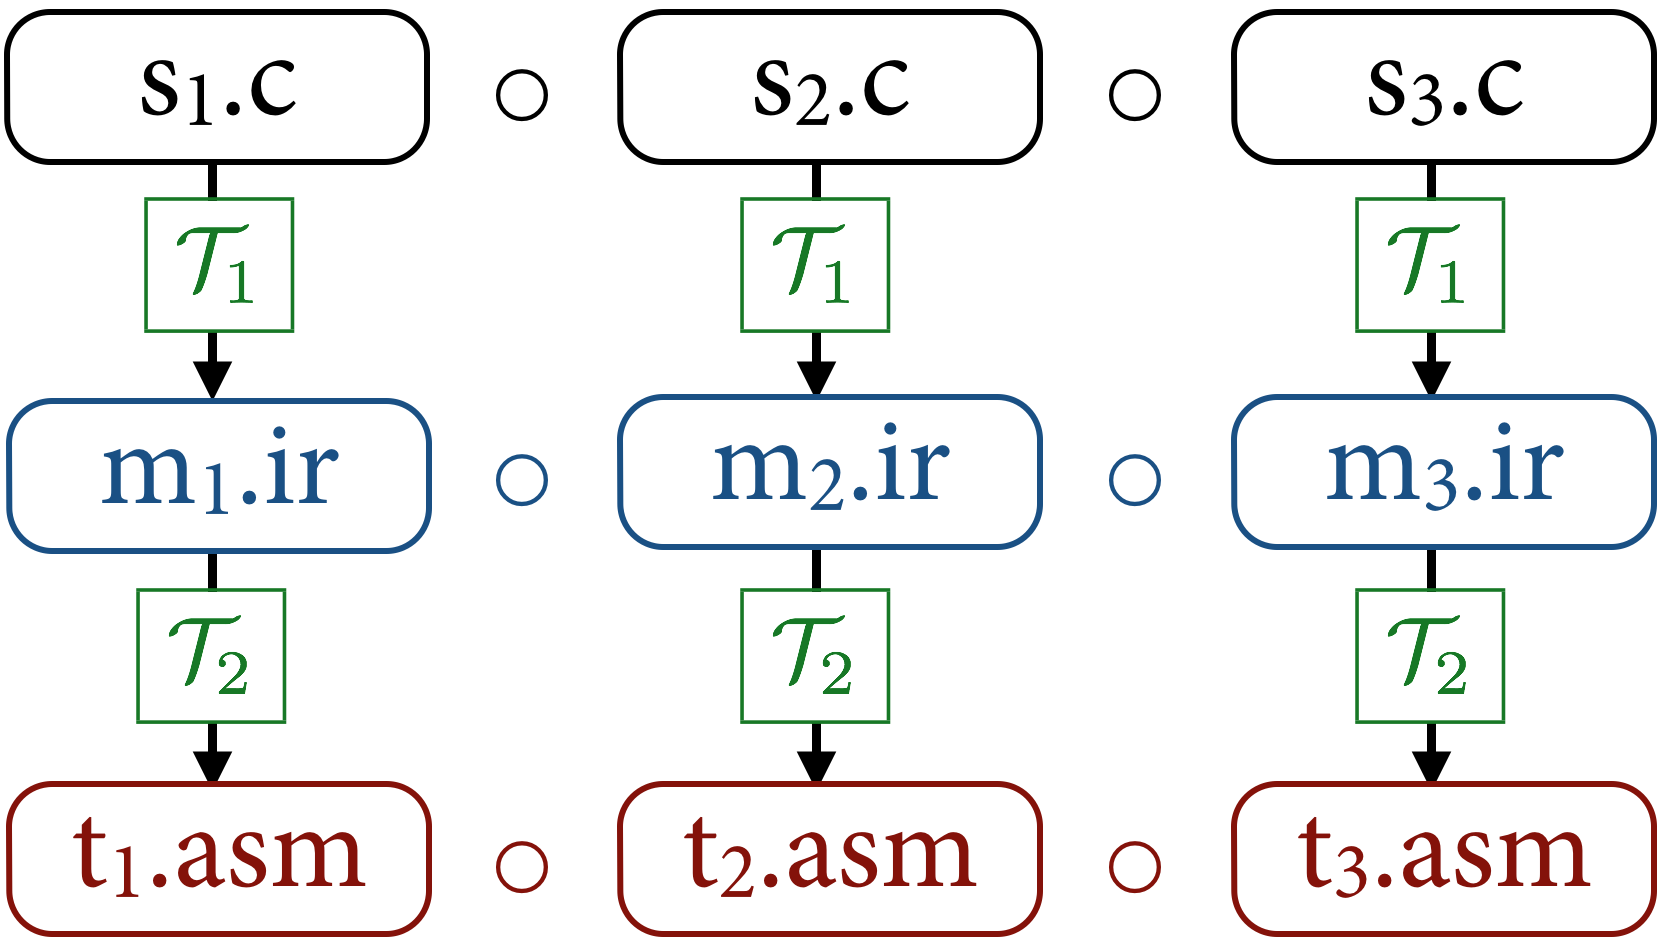
\includegraphics[width=200px]{sepcomp-levela.png}
\end{center}
\caption{Proving Level A correctness}
\label{fig:LevelA}
\end{figure}


\paragraph{End-to-End Correctness}

For Level A, we aim to show that if we separately compile $n$
different C modules
($\mathtt{s}_1\mathtt{.c},\ldots,\mathtt{s}_n\mathtt{.c}$) using the
same exact verified compiler $\mathcal{C}$, producing $n$ assembly
modules
($\mathtt{t}_1\mathtt{.asm},\ldots,\mathtt{t}_n\mathtt{.asm}$), then
the assembly-level linking of the $\mathtt{t}_i$'s will refine the
C-level linking of the $\mathtt{s}_i$'s.  Formally:
\[
\frac{
\begin{array}{@{}c@{}}
\forall i\in\setofz{1\ldots n}.~\mathcal{C}(\mathtt{s}_i\mathtt{.c}) = \mathtt{t}_i\mathtt{.asm} \\
s = \mathrm{load}(\mathtt{s}_1\mathtt{.c}\circ \ldots \circ \mathtt{s}_n\mathtt{.c})\qquad
t = \mathrm{load}(\mathtt{t}_1\mathtt{.asm}\circ \ldots \circ \mathtt{t}_n\mathtt{.asm})
\end{array}
}
{\mathrm{Behav}(s) \supseteq \mathrm{Behav}(t)}
\]
Here, $\circ$ represents simple \emph{syntactic} linking, \ie
essentially concatenation of files (plus checks to make sure that
externally declared variables/functions have the expected types).  See
\S\ref{sec:adaptconstprop} for further details about syntactic
linking.
% \footnote{See \S\ref{??} for further details about syntactic
%   linking.  Such a trivial notion of linking is no longer possible in
%   the recently released CompCert 2.5, due to the introduction of
%   support for \cd{static} variables.  See \S\ref{sec:related} for
%   further discussion of this point.}

\newcommand{\mys}[1]{\mathtt{s}_{#1}}
\newcommand{\myt}[1]{\mathtt{t}_{#1}}

\paragraph{Per-Pass Correctness}

To prove that compiler $\mathcal{C}$ satisfies Level A compositional correctness, we again want to
reduce the problem to one of verifying the individual passes of $\mathcal{C}$.  The key idea here,
as illustrated in Figure~\ref{fig:LevelA} where three separately-compiled modules go through two
compiler passes $\mathcal{T}_1$ and $\mathcal{T}_2$, is that since we know that the source modules
are all compiled via the exact same sequence of passes, we can verify their compilations in lock
step as if each pass is applied to all modules simultaneously.  In other words, it suffices to
verify that, for each pass $\mathcal{T}$ from $L_1$ to $L_2$, the following holds:
% Here, we show the case of three separately-compiled modules and two compiler passes,
% $\mathcal{T}_1$ and $\mathcal{T}_2$.  Since the compilations march in lock step, we can verify
% each pass as applied to all modules simultaneously.
\[
\frac{
\begin{array}{@{}c@{}}
\forall i\in\setofz{1\ldots n}.~\mathcal{T}(\mathtt{s}_i\mathtt{.l1}) = \mathtt{t}_i\mathtt{.l2} \\
s = \mathrm{load}(\mathtt{s}_1\mathtt{.l1}\circ \ldots \circ \mathtt{s}_n\mathtt{.l1})\qquad
t = \mathrm{load}(\mathtt{t}_1\mathtt{.l2}\circ \ldots \circ \mathtt{t}_n\mathtt{.l2})
\end{array}
}
{
\mathrm{Behav}(s) 
\supseteq \mathrm{Behav}(t)
}
\]
As before, these per-pass correctness results can be transitively
composed to immediately conclude end-to-end correctness of
$\mathcal{C}$.

\paragraph{Verifying Per-Pass Correctness}
So how do we prove this Level A per-pass correctness condition?
Assuming that we have already proven whole-program per-pass correctness
and are trying to port the proof over, there are two cases.

\textbf{Trivial case:} Many compiler passes are inherently
compositional, transforming the code of each module independently, \ie
in a way that is agnostic to the presence of other modules.  Put
another way, such compiler passes commute with linking:
\[
\mathcal{T}(\mathtt{s}_1\mathtt{.l1})\circ \ldots \circ \mathcal{T}(\mathtt{s}_n\mathtt{.l1}) = \mathcal{T}(\mathtt{s}_1\mathtt{.l1}\circ \ldots \circ \mathtt{s}_n\mathtt{.l1})
\]
If this commutativity property holds for a pass $\mathcal{T}$, then
Level A per-pass correctness becomes a trivial corollary of
whole-program per-pass correctness, where we instantiate the \cd{s.l1}
from \S\ref{sec:overview:compcert} with $\mathtt{s}_1\mathtt{.l1}\circ
\ldots \circ \mathtt{s}_n\mathtt{.l1}$.  In verifying Level A
correctness for CompCert 2.4, we found that 13 of its 19 passes fell
into this trivial case.

\textbf{Non-trivial case:} If the trivial commutativity argument does
not apply, then there is some new work to do to port a proof of
whole-program per-pass correctness to Level A per-pass correctness.

However, at least for CompCert, we found it very easy to perform this
adaptation.  Why?  First of all, since Level A correctness assumes
that all modules in the program are transformed in the same way, we
can essentially reuse the simulation relation $R$ for pass
$\mathcal{T}$ that was used in the original CompCert verification.

We do, however, have to worry about the soundness of the program
analyses that the compiler performs, because the correctness of the
compiler rests to a large extent on the correctness of these analyses.
To prove Level A correctness of these analyses, we must prove that
they remain sound even when they only have access to a single module
in the program rather than the whole program.  Intuitively, this
should follow easily if: (1) the analyses have been proven sound under
the assumption that they are fed the whole program (CompCert has done
that already), \emph{and} (2) the analyses are \emph{monotone},
meaning that they only become \emph{more conservative} when given
access to a smaller fragment of the program (as happens with separate
compilation).

In adapting CompCert to Level A correctness, the main work was
therefore in verifying that its program analyses were indeed monotone.
This was largely straightforward, with one exception: the ``value
analysis'' employed by several optimizations was not monotone.  It
made an assumption about variables declared as \cd{extern const},
which was valid for whole-program compilation, but not in the presence
of separate compilation.  As we explain in detail in
\S\ref{sec:adaptconstprop}, this manifested itself as a bug in
constant propagation when linking separately-compiled files.  After we
fixed this bug in value analysis, monotonicity became straightforward
to show, and thus so did Level A correctness (for the remaining 6
passes that did not fall into the trivial case).








% Or not:

% \[
% \frac{
% \begin{array}{@{}c@{}}
% \mathcal{T}(\mathtt{s}_1\mathtt{.l1})\circ \ldots \circ \mathcal{T}(\mathtt{s}_n\mathtt{.l1}) = \mathcal{T}(\mathtt{s}_1\mathtt{.l1}\circ \ldots \circ \mathtt{s}_n\mathtt{.l1})\\
% \mathtt{s.l1} = \mathtt{s}_1\mathtt{.l1}\circ \ldots \circ \mathtt{s}_n\mathtt{.l1}
% \\
% \mathtt{t.l2} = \mathcal{T}(\mathtt{s.l1})\qquad
% s = \mathrm{load}(\mathtt{s.l1})\qquad
% t = \mathrm{load}(\mathtt{t.l2})
% \end{array}
% }
% {
% \mathrm{Behav}(s) 
% \supseteq \mathrm{Behav}(t)
% }
% \]


\subsection{Compositional Correctness Level B}
\label{sec:overview:LevelB}

\begin{figure}[!t]
\begin{center}
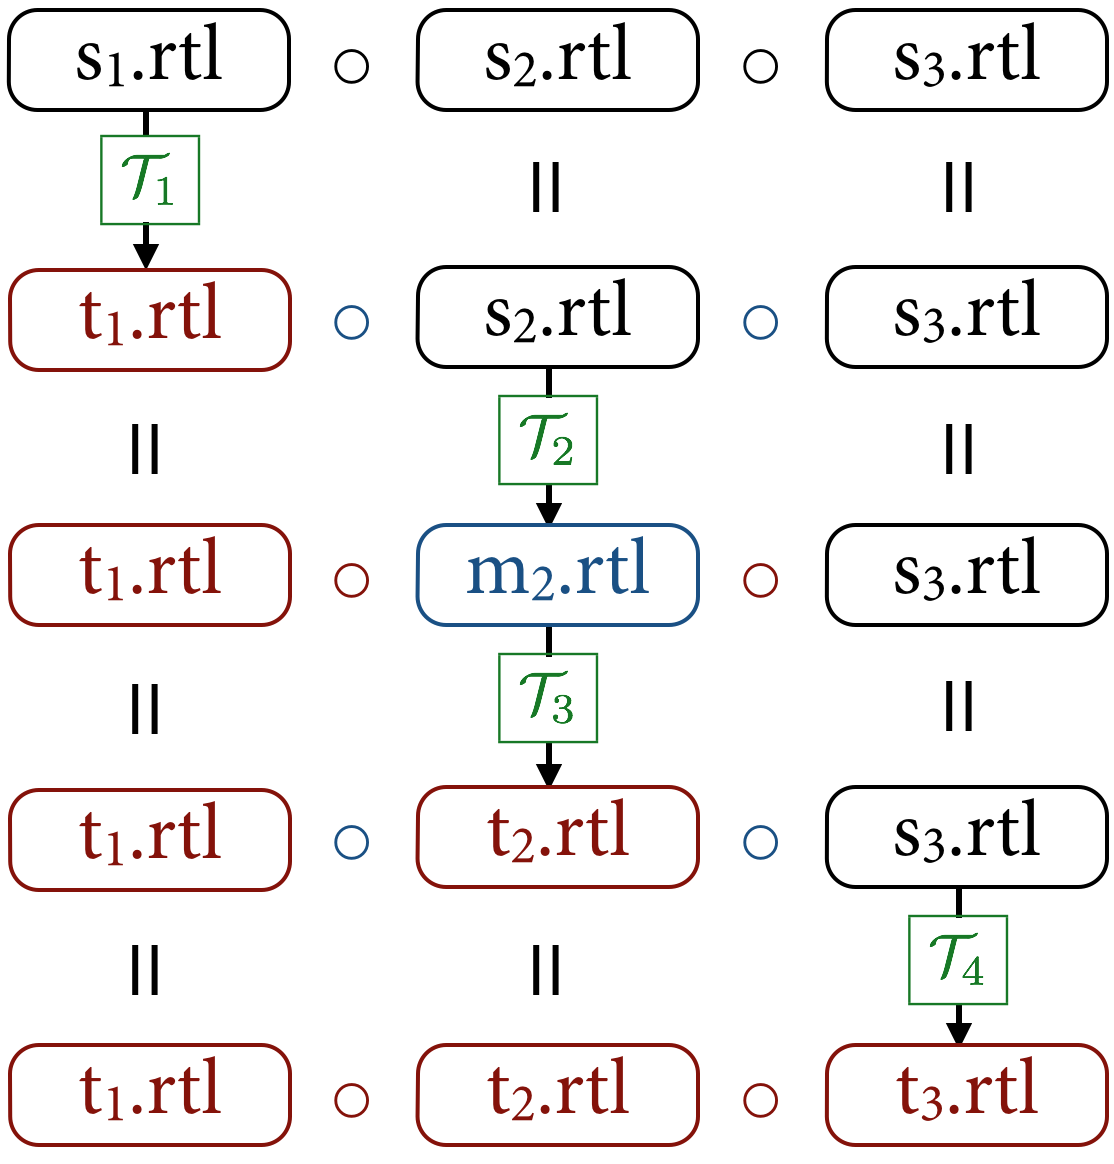
\includegraphics[width=200px]{sepcomp-levelb.png}
\end{center}
\caption{Proving Level B correctness for RTL passes}
\label{fig:LevelB}
\end{figure}
% Here, we show only the RTL-level passes (for other passes, it is the same as Level A).  Since each
% module is compiled with different optimization passes, we verify each pass applied to exactly one
% module, while simultaneously the other modules undergo the identity transformation.

\paragraph{End-to-End Correctness}

The CompCert compiler performs several key optimizations at the level
of its RTL intermediate language (\ie they are transformations from
RTL to RTL).  For Level B, we would like to strengthen Level A
correctness by allowing each source module $\mys{i}$ to be compiled by
a \emph{different} compiler $\mathcal{C}_i$.  However, the differences
we permit between the $\mathcal{C}_i$'s are restricted: they may
differ only in which optimization passes they apply at the RTL level.
Given this restriction on the $\mathcal{C}_i$'s, the Level B
correctness statement is the same as the Level A correctness statement
except for the replacement of $\mathcal{C}$ with $\mathcal{C}_i$:
\[
\frac{
\begin{array}{@{}c@{}}
\forall i\in\setofz{1\ldots n}.~\mathcal{C}_i(\mathtt{s}_i\mathtt{.c}) = \mathtt{t}_i\mathtt{.asm} \\
s = \mathrm{load}(\mathtt{s}_1\mathtt{.c}\circ \ldots \circ \mathtt{s}_n\mathtt{.c})\qquad
t = \mathrm{load}(\mathtt{t}_1\mathtt{.asm}\circ \ldots \circ \mathtt{t}_n\mathtt{.asm})
\end{array}
}
{
\mathrm{Behav}(s) 
\supseteq \mathrm{Behav}(t)
}
\]

\paragraph{Per-Pass Correctness}

To verify the above correctness statement, we yet again want to reduce
it to verifying the individual passes of $\mathcal{C}$.  For all passes
besides the RTL-level optimizations, we can verify per-pass
correctness exactly as in Level A, since all the $\mathcal{C}_i$'s must
perform these same passes in the same order.  However, for the RTL
optimizations, we must do something different because at the RTL level
the various $\mathcal{C}_i$'s do not all march in lock step.

The key idea for handling the RTL optimizations, as illustrated in Figure~\ref{fig:LevelB} where
each module is compiled with different optimization passes, is to pad the $\mathcal{C}_i$'s with
extra dummy identity passes (which do not affect their end-to-end functionality) so that, whenever
one compiler is performing an RTL optimization pass, the other compilers will for that step perform
an identity transformation.  Thus, we first verify the RTL passes of $\mathcal{C}_1$ in parallel
with identity passes for the other compilers, then verify the RTL passes of $\mathcal{C}_2$ in
parallel with identity passes for the other compilers, and so on.  For this to work, the Level B
per-pass correctness statement (for optimization passes $\mathcal{T}$ from RTL to RTL) must be
updated as follows:
\[
\frac{
\begin{array}{@{}c@{}}
\mathcal{T}(\mathtt{s.rtl}) = \mathtt{t.rtl} \\
\!s = \mathrm{load}(\mathtt{u}_1\mathtt{.rtl}\circ \ldots \circ \mathtt{u}_m\mathtt{.rtl}\circ\mathtt{s.rtl} \circ \mathtt{v}_1\mathtt{.rtl}\circ \ldots \circ \mathtt{v}_n\mathtt{.rtl})\\
t = \mathrm{load}(\mathtt{u}_1\mathtt{.rtl}\circ \ldots \circ \mathtt{u}_m\mathtt{.rtl}\circ\mathtt{t.rtl}\circ \mathtt{v}_1\mathtt{.rtl}\circ \ldots \circ \mathtt{v}_n\mathtt{.rtl})
\end{array}
}
{
\mathrm{Behav}(s) 
\supseteq \mathrm{Behav}(t)
}
\]
One can view this notion of per-pass correctness as being essentially
a form of \emph{contextual refinement}: the output of $\mathcal{T}$
must refine its input when linked with a context consisting of some
arbitrary other RTL modules (the $\mathtt{u}_i$'s and
$\mathtt{v}_j$'s).  If we can prove this, it should be clear from
Figure~\ref{fig:LevelB} how the per-pass proofs link up transitively.

\paragraph{Verifying Per-Pass Correctness}

So how do we prove this contextual refinement?  Unlike for Level A, we
cannot simply reuse the existing simulation $R$ from the whole-program
per-pass correctness proof for $\mathcal{T}$, because $R$ is not
necessarily reflexive and thus does not necessarily relate the
execution of code from $\mathtt{u}_i\mathtt{.rtl}$ (or
$\mathtt{v}_j\mathtt{.rtl}$) with itself.  Instead, we must use an
amended simulation $R'$, which accounts for two possibilities: either
we are executing code from \cd{s} on one side of the simulation and
code from \cd{t} on the other, in which case the proof that $R'$ is
indeed a simulation proceeds essentially as did the proof that $R$
was a simulation; or we are executing code from
$\mathtt{u}_i\mathtt{.rtl}$ (or $\mathtt{v}_j\mathtt{.rtl}$), in which
case both sides of the simulation are executing exactly the same
RTL instructions.

In principle, the latter case could involve serious new proof effort.
However, at least for CompCert, we found that in fact the substance of
this new part of the proof was hiding in plain sight within the
original CompCert verification!  The reason, intuitively, is that
RTL-to-RTL optimization passes are rarely unconditional
transformations: their output typically only differs from their input
\emph{when certain conditions (e.g. determined by a static analysis)
  hold}, and since these conditions do not always hold, these passes
may end up leaving any given input instruction unchanged.  To account
for this possibility, the original CompCert verification must
therefore already prove that arbitrary RTL instructions simulate
themselves.  Consequently, in porting CompCert 2.4 to Level B
compositional correctness, we were able to simply extract and compose
(essentially, copy-and-paste) these micro-simulation proofs into the
simulation proof for the latter part of $R'$.






%%%%%%%%%%%%%%%%%%%%%%%%%%%

% \section*{Key Results}

% We present techniques for compiler verification whose key results are as follows.

% % \paragraph{Part 1}
% % \[
% % \frac{
% % \begin{array}{@{}c@{}}
% % \forall i\in\setofz{1\ldots n}.~\mathtt{t}_i\mathtt{.asm} = \mathcal{C}(\mathtt{s}_i\mathtt{.c})\\
% % s = \mathrm{load}(\mathtt{s}_1\mathtt{.c}\circ \ldots \circ \mathtt{s}_n\mathtt{.c})\qquad
% % t = \mathrm{load}(\mathtt{t}_1\mathtt{.asm}\circ \ldots \circ \mathtt{t}_n\mathtt{.asm})
% % \end{array}
% % }
% % {\mathrm{Behav}(s) \supseteq \mathrm{Behav}(t)}
% % \]
% % where $\circ$ is the syntactic linking and $\mathcal{C}$ is a verified compiler.


% \paragraph{Part 2}
% \[
% \frac{
% \begin{array}{@{}c@{}}
% \forall i\in\setofz{1\ldots n}.~\mathtt{t}_i\mathtt{.asm} = \mathcal{C}_i(\mathtt{s}_i\mathtt{.c})\\
% s = \mathrm{load}(\mathtt{s}_1\mathtt{.c}\circ \ldots \circ \mathtt{s}_n\mathtt{.c})\qquad
% t = \mathrm{load}(\mathtt{t}_1\mathtt{.asm}\circ \ldots \circ \mathtt{t}_n\mathtt{.asm})
% \end{array}
% }
% {
% \mathrm{Behav}(s) 
% \supseteq \mathrm{Behav}(t)
% }
% \]
% where $\circ$ is the syntactic linking and
% $\mathcal{C}_i$'s are verified compilers that differ only in optimization passes from RTL to RTL.

% % \paragraph{Part 3}
% % \[
% % \frac{
% % \begin{array}{@{}c@{}}
% % \forall i\in\setofz{1\ldots n}.~\mathtt{t}_i\mathtt{.asm} = \mathcal{C}_i(\mathtt{s}_i\mathtt{.c})\\
% % \hspace*{-1.7pc}
% % s = \mathrm{load}(\mathtt{u}_1\mathtt{.asm}\bullet\ldots\bullet\mathtt{u}_m\mathtt{.asm}\bullet
% % \mathtt{s}_1\mathtt{.c}\bullet \ldots \bullet \mathtt{s}_n\mathtt{.c})\\
% % t = \mathrm{load}(\mathtt{u}_1\mathtt{.asm}\bullet\ldots\bullet\mathtt{u}_m\mathtt{.asm}\bullet\mathtt{t}_1\mathtt{.asm}\bullet \ldots \bullet \mathtt{t}_n\mathtt{.asm})
% % \end{array}
% % }
% % {
% % \mathrm{Behav}(s) \supseteq \mathrm{Behav}(t)
% % }
% % \]
% % where $\bullet$ is the interaction semantics linking and
% % $\mathcal{C}_i$'s are aribtrary verified compilers.

% % We present our verification techniques.

% % \paragraph{Part 1}



% % For each optimization pass $\mathcal{T}$ from a language $L_1$ to $L_2$,
% % we show the following:
% % \[
% % \frac{
% % \begin{array}{@{}c@{}}
% % \mathcal{T}(\mathtt{s}_1\mathtt{.l1})\circ \ldots \circ \mathcal{T}(\mathtt{s}_n\mathtt{.l1}) = \mathcal{T}(\mathtt{s}_1\mathtt{.l1}\circ \ldots \circ \mathtt{s}_n\mathtt{.l1})\\
% % \mathtt{s.l1} = \mathtt{s}_1\mathtt{.l1}\circ \ldots \circ \mathtt{s}_n\mathtt{.l1}
% % \\
% % \mathtt{t.l2} = \mathcal{T}(\mathtt{s.l1})\qquad
% % s = \mathrm{load}(\mathtt{s.l1})\qquad
% % t = \mathrm{load}(\mathtt{t.l2})
% % \end{array}
% % }
% % {\exists R.~ \mathrm{simulation}~R \land 
% % (s,t)\in R
% % }
% % \]

% % Or

% % \[
% % \frac{
% % \begin{array}{@{}c@{}}
% % \forall i\in\setofz{1\ldots n}.~\mathtt{t}_i\mathtt{.l2} = \mathcal{T}(\mathtt{s}_i\mathtt{.l1})\\
% % s = \mathrm{load}(\mathtt{s}_1\mathtt{.l1}\circ \ldots \circ \mathtt{s}_n\mathtt{.l1})\qquad
% % t = \mathrm{load}(\mathtt{t}_1\mathtt{.l2}\circ \ldots \circ \mathtt{t}_n\mathtt{.l2})
% % \end{array}
% % }
% % {\exists R.~ \mathrm{simulation}~R \land 
% % (s,t)\in R
% % }
% % \]

% \paragraph{Part 2}

% For each optimization pass $\mathcal{T}$ from RTL to RTL,
% we show the following:
% \[
% \frac{
% \begin{array}{@{}c@{}}
% \mathtt{t.r} = \mathcal{T}(\mathtt{s.r})\\
% \!s = \mathrm{load}(\mathtt{u}_1\mathtt{.r}\circ \ldots \circ \mathtt{u}_n\mathtt{.r}\circ\mathtt{s.r})\\
% t = \mathrm{load}(\mathtt{u}_1\mathtt{.r}\circ \ldots \circ \mathtt{u}_n\mathtt{.r}\circ\mathtt{t.r})
% \end{array}
% }
% {\exists R.~ \mathrm{simulation}~R \land 
% (s,t)\in R
% }
% \]
% For other optimization passes, we use the verification technique of Part 1.

% \paragraph{Part 3}

% %% \ge^\mathrm{u}_\mathrm{C,Asm}

% For each optimization pass $\mathcal{T}$ from a language $L_1$ to $L_2$,
% we show the following:
% \[
% \frac{
% \begin{array}{@{}c@{}}
% \mathtt{t.l2} = \mathcal{T}(\mathtt{s.l1})\\
% \!s = \mathrm{load}(\mathtt{u}_1\mathtt{.c}\bullet \ldots \bullet \mathtt{u}_n\mathtt{.c}\bullet\mathtt{v}_1\mathtt{.asm}\bullet \ldots \bullet \mathtt{v}_m\mathtt{.asm}\bullet\mathtt{s.l1})\\
% t = \mathrm{load}(\mathtt{u}_1\mathtt{.c}\bullet \ldots \bullet \mathtt{u}_n\mathtt{.c}\bullet\mathtt{v}_1\mathtt{.asm}\bullet \ldots \bullet \mathtt{v}_m\mathtt{.asm}\bullet\mathtt{t.l2})
% \end{array}
% }
% {\exists R.~ \mathrm{simulation}~R \land 
% (s,t)\in R
% }
% \]


%%% Local Variables:
%%% mode: latex
%%% TeX-master: "main"
%%% TeX-command-extra-options: "-shell-escape"
%%% End:

\section{Running Example: Constant Propagation}
\label{sec:sepcomp:constprop}

In this section, we explain how to adapt the CompCert proof of
constant propagation to support separate compilation.  Before doing
so, let us briefly explain syntactic linking in some more detail since
it is central to the compositional correctness results we prove.

Syntactic linking merges global declarations for each identifier.
The linker must check if the declarations meet the following conditions:
\begin{itemize}
\item The declarations have the same type.  They should be either
  $(i)$ function declarations or definitions of the same signature, or
  $(ii)$ variable declarations or definitions of the same type.
\item At most one of the declarations is a definition.  If there is a
  single definition, then that is the result of the linking;
  otherwise, everything is necessarily the same declaration, and that
  is the result of the linking.
\end{itemize}
\noindent We have generically defined syntactic linking for all the
languages used in CompCert, as it does not depend on specific language
features.

% Next, we describe how we can adapt the CompCert proof of constant propagation to achieve separate compilation.

\subsection{Verifying Compositional Correctness Level A}

\paragraph{Adapting the Simulation Relation Definition}

To verify compositional correctness Level A, we will---as in the
original CompCert proof---construct a simulation relation $R$ that
relates the initial states of the source and target programs.  The
difference is that the source program consists of multiple files, each
of which is separately compiled.
\[
\frac{
\begin{array}{@{}c@{}}
\vprg = \mathtt{s}_1\circ \ldots \circ \mathtt{s}_n \qquad
\vprg' = \mathcal{T}_\mathrm{cp}(\mathtt{s}_n)\circ \ldots \circ \mathcal{T}_\mathrm{cp}(\mathtt{s}_n)
\end{array}
}
{\exists R.~ \mathrm{simulation}~R \land (\rtlload(\vprg),\rtlload(\vprg'))\in R
}
\]
Therefore, for each function definition ($\vfd$) in the source program
($\vprg$), the corresponding function definition ($\vfd'$) in the
target program ($\vprg'$) is no longer obtained by
$\mathrm{transfun}(\vprg,\vfd)$, but rather by
$\mathrm{transfun}(\mathtt{s}_i,\vfd)$ for some subprogram
$\mathtt{s}_i$ of $\vprg$.  Moreover, the value analysis run as part
of $\mathrm{transfun}$ also gets a subprogram of $\vprg$ as its first
argument.

Consequently, the simulation relation we use for the proof of soundness has to change.
The main change is, naturally, in the definition of $\simFun$.
Two function definitions are now related if the second can be obtained by transforming the first in the context of a subprogram of $\vprg$.
\[ 
\vprg \vdash \vfd \simFun \vfd' ~\defeq~ \exists \vsprg \subseteq \vprg.~ \vfd' = \mathrm{transfun}(\vsprg,\vfd)
\]
where $\vsprg \subseteq \vprg$ iff $\exists \vsprg'.~\vsprg \circ
\vsprg' = \vprg$.\footnote{In the Coq development, we define $\vsprg
  \subseteq \vprg$ in an equivalent but more direct, semantic way,
  rather than relying on syntactic linking ($\circ$).  This enables us
  to avoid having to prove associativity and commutativity of
  linking.}

The second change is to decouple the two uses of $\vprg$ in $\soundstate$,
changing its signature so that it takes three arguments: two programs $\vprg$ and $\vsprg$, and a state $s$.
The first program, $\vprg$, corresponds to the full program and is used to calculate the global environment,
whereas the second program, $\vsprg$, is a subprogram of the first one and is used to perform the global analysis
(\ie to detect which variables are constant). 

We then define a wrapper predicate $\soundstate'$ as follows:
\[
\soundstate'(\vprg,s) ~\defeq~ 
  \forall \vsprg \subseteq \vprg.~ \soundstate(\vprg,\vsprg,s)
\]
and change $R$ to use $\soundstate'$ instead of $\soundstate$.

%A final difference is that also have to parametrize the simulation relation by the target program, $\vprg'$
%is preserved by constant propagation.

\paragraph{Adapting the Proof of Value Analysis}

There are multiple proofs that require adaptation.
First, we have to prove that value analysis is correct with respect to our stronger invariant.
That is, we have to show that $\soundstate'$ holds of the initial state of a loaded program and that it is preserved by execution steps.

The latter requirement is actually trivial to show and requires only
very minor changes to the CompCert proof script.  The reason for this,
informally, is that the uses of the $\vprg$ and $\vsprg$ parameters in
the revised $\soundstate$ invariant are really decoupled and that the
preservation proof never depends on them being the same.

% \input{constprop-bug} TODO

The former requirement, however, requires some more work:
not only should $\soundstate(\vprg,\vprg,\load(\vprg))$ hold for all programs $\vprg$,
but rather $\soundstate(\vprg,\vsprg,\load(\vprg))$ should hold for all programs $\vprg$ and all subprograms $\vsprg\subseteq\vprg$.
In essence, to satisfy this stronger statement, the additional requirement that we have to show is that value analysis is monotone with respect to linking.
That is, for each global variable \texttt{x}, we prove
\[
\vsprg \subseteq \vprg \implies  \mathrm{abs\text{-}val}(\vsprg,\texttt{x}) \sqsupseteq \mathrm{abs\text{-}val}(\vprg,\texttt{x})
\]
where $\mathrm{abs\text{-}val}(\vprg,\texttt{x})$ is the abstract value of \texttt{x} computed by the global analysis on $\vprg$.
In other words, running the analysis on a larger program may only give results that are at least as precise.

Somewhat surprisingly, (the global part of) the value analysis in
CompCert 2.4 does not satisfy this monotonicity requirement because of
its treatment of variables declared as both \cd{extern} and
\cd{const}.  Figure~\ref{fig:constprop-bug} presents two C files that,
when compiled separately and linked together, expose the bug.  Since
the global variable \cd{xptr} is declared using the \cd{const}
qualifier, the global part of CompCert 2.4's value analysis assumes
that it is uninitialized and therefore assigns it the abstract value
$\bot$.  As a result, the value analysis deems that \cd{xptr} cannot
possibly alias with \texttt{x}.  At the \cd{printf} statement, it
hence deduces that $\texttt{x}=1$, and constant propagation
``optimizes'' away the summation \cd{x+x} to the constant $2$, which
gets printed.  This analysis, however, is unsound.  In particular, the
assumption that \cd{xptr} is uninitialized is invalid in the context
of multiple separately compiled files: since \cd{xptr} is also
declared as \cd{extern}, another file (\cd{b.c}) can provide a
definition that initializes it.  And indeed, since the definition of
\cd{xptr} in \cd{b.c} causes \cd{x} and \cd{xptr} to alias, the
correct result is $0$, not $2$.

Restoring soundness of the value analysis is straightforward: one
simple if rather crude fix (which has been adopted by CompCert 2.5
since we reported the bug) is just to ignore the \cd{const} modifier
on \cd{extern} declarations.  Having done that, it is easy to show
that the analysis is monotone with respect to program linking and that
therefore the initial state of loading a program satisfies the
stronger invariant $\soundstate'(\vprg,\load(\vprg))$.


\paragraph{Adapting the Proof of Constant Propagation}

Showing that constant propagation is sound requires only very little additional work.

The only important difference is in the treatment of global environments that index the $\estep{}$ relation.
Generally, these environments are obtained by the respective programs ($ge=\rtlgenv(\vprg)$ and $ge'=\rtlgenv(\vprg')$). 

The original CompCert 2.4 proof used the fact that
$\vprg'=\mathcal{T}_{\rm cp}(\vprg)$ to establish a relationship
between $ge$ and $ge'$.  It proved two basic properties relating the
two global environments: (1) that they map each global variable name
to the same block identifier, and (2) that if $ge$ maps a block
identifier to a function signature or definition $\vfds$, then $ge'$
maps it to $\mathrm{transfun}(\vprg,\vfds)$, where $\mathrm{transfun}$
applied to a function signature returns the same signature.  These
lemmas were then used in the proof that $R$ is a simulation relation.

Since, now, the relationship between $\vprg$ and $\vprg'$ is more involved, 
we have to update the proof of the first lemma, which is rather straightforward,
as well as the statement and proofs of the second lemma.
For the second lemma, we now assert that 
if $ge$ maps a block identifier to a function signature or definition $\vfds$, 
then $ge'$ maps it to $\mathrm{transfun}(\vsprg,\vfds)$ for \emph{some} subprogram $\vsprg\subseteq\vprg$.
Besides this change, 
the proof that now (the new definition of) $R$ is a simulation relation is basically unchanged.
The few lines of the proof script that required editing were those invoking the lemmas about the relationship between the global environments.


\subsection{Verifying Compositional Correctness Level B}

\paragraph{Adapting the Simulation Relation Definition}

We move on to verifying the second level of compositional correctness, that of composition with the same compiler modulo optimization flags.
As we have explained in \S\ref{sec:overview:LevelB}, for every optional optimization pass, we need to show that linking it against the identity compiler is sound.
Since constant propagation is one of the optional optimization passes, we have to prove the following:
\[
\frac{
\begin{array}{@{}r@{~}l@{}}
\vprg &= \mathtt{u}_1\circ \ldots \circ \mathtt{u}_m\circ\mathtt{s} \circ \mathtt{v}_1\circ \ldots \circ \mathtt{v}_n\\
\vprg' &= \mathtt{u}_1\circ \ldots \circ \mathtt{u}_m\circ\mathcal{T}_{\rm cp}(\mathtt{s}) \circ \mathtt{v}_1\circ \ldots \circ \mathtt{v}_n
\end{array}
}
{\exists R.~ \mathrm{simulation}~R \land 
(\rtlload(\vprg),\rtlload(\vprg'))\in R
}
\]
In the scenario above, the corresponding target function definition $\vfd'$ of a source function definition $\vfd$
is either syntactically identical to $\vfd$ if it belongs to one of the $\mathtt{u}_i$/$\mathtt{v}_j$ files, 
or has been obtained by optimizing $\vfd$ if it belongs to the $\mathtt{s}$ file.
To account for the change, we should therefore redefine the $\simFun$ relation as follows:
\[ 
\begin{array}{l}
\vprg \vdash \vfd \simFun \vfd' ~\defeq~ 
\\\qquad\qquad
\vfd' = \vfd \lor (\exists \vsprg \subseteq \vprg.~ \vfd' = \mathrm{transfun}(\vsprg,\vfd))
\end{array}
\]
This is the only change needed in the simulation relation.

%% \[
%%  \frac{
%% \begin{array}{c}
%% \vfd = \vfd' \qquad
%%  rs \le_\rtldef rs'
%% \end{array}
%%  }
%%  {
%% \vprg \vdash (r,\vfd,sp,pc,rs) \simFrame (r,\vfd',sp,pc,rs')
%%  }
%% \]

%% \[
%%  \frac{
%% \begin{array}{c}
%%  m \sqsubseteq_\mathrm{ext}  m' \quad
%%  s \simStack s' \quad
%% \vfd = \vfd' \quad
%%  rs \le_\rtldef rs'
%% \end{array}
%%  }
%%  {
%% \vprg \vdash
%% \rtlist~m~s~\vfd~sp~pc~rs \simState
%% \rtlist~m'~s'~\vfd'~sp~pc~rs'
%%  }
%% \]


%% \[
%%  \frac{
%% \begin{array}{@{}c@{}}
%% m \sqsubseteq_\mathrm{ext}  m' \quad
%% s \simStack s' \quad
%% \vfd = \vfd' \quad
%% \vargs \le_\rtldef \vargs' 
%% \end{array}
%%  }
%%  {
%% \vprg \vdash
%% \rtlcst~m~s~\vfd~\vargs \simState 
%% \rtlcst~m'~s'~\vfd'~\vargs'
%%  }
%% \]

\paragraph{Adapting the Proof of Constant Propagation}

To avoid changing the proof script of the main lemma showing that $R$
is in fact a simulation, we prove a helper lemma
(\textit{transf\_step\_correct\_identical}) saying that, given two
matching instruction states with $\vfd'=\vfd$, when the source state
takes a step, the target state can also take a step and reach a
matching state.  As explained in \S\ref{sec:overview:LevelB}, the
content of the proof of this helper lemma is already present in the
existing simulation proof, just not in one place, so it simply needs
to be extracted and consolidated.  We then adapt the proof of the main
lemma (showing $R$ is a simulation) so that it performs a case split on
whether $\vfd=\vfd'$ or not, and correspondingly either invokes our
helper lemma or uses the same proof script as for Level A.


%%% Local Variables:
%%% mode: latex
%%% TeX-master: "main"
%%% TeX-command-extra-options: "-shell-escape"
%%% End:

\section{Verifying the Other Passes}

In the previous sections, we looked at the specific example of
constant propagation in detail and explained how we ported CompCert's
proof of that pass to \sepcomp{}'s Level A and B notions of
compositional correctness.  In this section, we discuss some details
of other CompCert passes for which porting to \sepcomp{} required some
interesting (but still not much) work.

\begin{figure*}[t]
\begin{center}
\includegraphics[scale=.5]{passes.png}
\end{center}
\caption{Optimization passes of \sepcomp{} Level A and Level B.}
\label{fig:sep-comp-passes}
\end{figure*}

Figure~\ref{fig:sep-comp-passes} shows which verification technique we
apply to each optimization pass of CompCert.  For Level A, we apply
the trivial technique based on commutativity with linking to 13 passes
and the non-trivial technique to 6 passes.  For Level B, we apply our
technique to all 6 RTL-to-RTL passes.

% % Since the trivial
% % case of Level A (when passes commute with linking) is, well, trivial,
% % we do not discuss it here.

% As explained in \S\ref{sec:overview:LevelA}, porting 13 of the 19
% passes of CompCert to Level A was trivial because those passes commute
% with syntactic linking.  For porting the remaining passes to Level A,
% and for porting all passes to Level B, we can update the proof, as we
% have seen, in three steps:
% \begin{enumerate}
% \item Update the simulation relation $R$.
% \item Update the proof that $R$ is in fact a simulation relation.
% \item Update the proof that the initial states after loading are
%   related by $R$.
% \end{enumerate}

% \paragraph{CompCert to Level A}

% The general idea for updating the simulation relation is to simply change the
% whole program $\vprg$ to a sub-program $\vsprg$ such that $\vsprg
% \subseteq \vprg$ whenever $\vprg$ is used as compile-time information.
% For example, for the constant propagation pass, we changed
% \[\vfd' = \mathrm{transfun}(\vprg,\vfd)\]
% to
% \[\exists \vsprg \subseteq \vprg.~
% \vfd' = \mathrm{transfun}(\vsprg,\vfd)\] 
% and
% \[
% \soundstate(\vprg,\vprg,s)\]
% to
% \[
% \forall \vsprg \subseteq \vprg.~
% \soundstate(\vprg,\vsprg,s)
% \]
% New proof obligations introduced by these changes essentially amount
% to establishing the monotonicity of various properties: that the
% property continues to hold in a larger program context than was used
% at compilation time.  In CompCert, it turned out that proving such
% monotonicity is quite easy.  We will discuss below what monotonicities
% we had to prove for each optimization in detail.

% \paragraph{Level A to Level B}

% The general idea for updating the simulation relation is to add a case
% to the simulation for when identical functions are invoked in the
% source and target. Here, we can easily derive such invariants as
% special cases from the invariants used in Level A because usual
% optimizations essentially subsume the possibility of nothing being
% optimized.

% New proof obligations introduced by theses updates are essentially
% special cases of existing ones and thus one can easily kill them by
% cut-and-pasting followed by specialization.  More specifically, while
% the original simulation proof shows step-simulation for states where
% only the source and optimized functions are invoked in the current
% state and all stack frames, now we have three more logical cases (\ie
% (current,stack frame) = (optimized,identical), (identical,optimized),
% (identical,identical)). In all RTL-to-RTL passes, we could easily
% adapt existing proofs for the original case (\ie (current,stack frame)
% = (optimized,optimized)) to the other three cases by cutting-and-paste
% and specialization, and thus there is nothing interesting to discuss.

%% However, 

%% the proof of step-simulation for the other three cases
%% ((current,stack frame) = (optimized,identical), (identical,optimized)
%% or (identical,identical)) is almost a special case of the original case
%% ((current,stack frame) = (optimized,optimized)).

%% More specifically,
%% we update the simulation proof as follows:
%% \begin{itemize}
%% \item
%% We first update the existing simulation proof to cover cases where

%% identical functions are 
%% stack frames 

%% when the optmized functions are currently executed.
%% This is easy because stack frames for identical functions are subsumed by
%% those for optmized functions.
%% \item
%% We prove the case where identical functions are currently executed
%% by copy-and-pasting the proof of the case where optimized functios are executed
%% and specializing them.
%% \item 
%% Showing that the initial memories are related is easy by construction.
%% \item
%% Code Refactoring
%% \end{itemize}

%% \todo{jeehoon: moved the descriptions for level B's general pattern
%%   from examples}
%% \begin{itemize}
%% \item match\_fundef : id or translated
%% \item identical case for match\_stacks, match\_identical\_states
%% \item Update lemmas for identical cases by copy-and-pasting.
%% \item Prove the step lemma for identical cases by copy-and-pasting:
%%   $T \to I$, $I \to T$, $ I \to I$ cases.
%% \end{itemize}

\subsection{RTL-Level Optimizations that Rely on Value Analysis}
Three RTL-level optimizations rely on the value analysis: constant
propagation, common subexpression elimination (CSE), and deadcode
elimination (DCE).  These passes are inter-procedural solely because
they rely on the value analysis.  Thus, the porting of the proofs of
CSE and DCE to support compositional correctness proceeded analogously
to the porting of the constant propagation pass.


\subsection{Selection}
The selection pass ``recognizes opportunities for using combined
arithmetic and logical operations and addressing modes offered by the
target processor.''~\cite{compcert-website}.  The pass is mostly
intra-procedural, except for the following two transformations on
function calls.

\paragraph{Recognizing Immediate Calls}
The selection pass transforms an indirect call via a function pointer
expression, say $e_p$, into an immediate call, if it can determine
that the expression $e_p$ always evaluates to the pointer to an
internal function.  The pass uses a simple analysis
$\texttt{classify\_call}(prg, e_p)$ for determining this.  For separate
compilation, we proved the monotonicity of the analysis: the result
$\texttt{classify\_call}(sprg, e_p)$ for a subprogram $sprg \subseteq
prg$ is sound w.r.t.\ the whole program $prg$.

\paragraph{64-bit Integer Operations into Library Calls}
The selection pass transforms some 64-bit integer operations into
calls to library helper functions.  For example, \texttt{(long long)
  f}, a cast from \texttt{float} to \texttt{long long}, is transformed
into a call \texttt{\_\_int64\_dtos(f)} to the corresponding helper
function.  For this transformation to be valid, the pass should ensure
that the helper function (\eg \texttt{\_\_int64\_dtos}) is
declared as an external function in the source program's global
environment.  CompCert has a designated checker
$\texttt{check\_helpers}(prg)$ to ensure this property.

For separate compilation, we proved that the checker for helper
functions is monotone w.r.t. linking: $\texttt{check\_helpers}(prg1)$
and $\texttt{check\_helpers}(prg2)$ implies
$\texttt{check\_helpers}(prg1 \circ prg2)$ for all programs $prg1$ and
$prg2$.  The proof is a little bit involved, as linking reorders
global declarations, and the corresponding logical blocks for the
helper functions in the global environments may vary.

% Note that the monotonicity we proved for \texttt{check\_helpers}
% deviates from the general pattern, namely ensuring
% $\texttt{check\_helpers}(sprg)$ for some $sprg \subseteq prg$.  This
% is because the context $ctx$ of $sprg$, which satisfies
% $sprg \circ ctx = prg$, may redefine library helper functions as
% internal functions, and invalidate the properties on helper functions
% in the whole-program $prg$.

\paragraph{Compiler Bug We Found}
The original CompCert 2.4 used a function $\texttt{get\_helpers}$
instead of $\texttt{check\_helpers}$.  We found and reported a
compiler bug related to $\texttt{get\_helpers}$, which was
subsequently confirmed.
% \footnote{See the README of the supplementary
  % materials for more details.}

We found the bug in the course of proving monotonicity regarding
$\texttt{get\_helpers}$. This function is directly implemented in
OCaml and its property is axiomatized in Coq as follows.
%\newpage
\begin{verbatim}
Axiom get_helpers_correct:
  forall ge hf, get_helpers ge = OK hf ->
  i64_helpers_correct ge hf.
\end{verbatim}
The problem was that this axiom is not strong enough to prove
monotonicity, and even worse, not true for the OCaml implementation of
$\texttt{get\_helpers}$. One of the properties this axiom postulates
is that helper functions like \texttt{\_\_int64\_dtos} are only
declared but not defined in the source program. However,
$\texttt{get\_helpers}$ does not check it at compile time!

Here is an example that exposes the bug.
\begin{verbatim}
#include <stdio.h>
long long __i64_dtos(float t) {
  return 3;
}
int main() {
  // expected: 5, actual: 3
  printf(“%lld\n”, (long long) 5.0f);
  return 0;
}
\end{verbatim}
Here the cast \texttt{(long long) 5.0f} is converted to a call to the
library helper function \texttt{\_\_i64\_dtos(5.0f)} by the selection
pass. However, we successfully hijack the function call by overwriting
the function \texttt{\_\_i64\_dtos}, which results in printing $3$
instead of the correct result $5$.  Now, strictly speaking, due to the
hijacking of a reserved identifier, this example has undefined
semantics according to the C99 standard, so CompCert's behavior here
is technically legal.  But the dependence on an invalid axiom is
clearly a bug.

After we reported this bug, it was fixed in the development branch of
CompCert (and subsequently CompCert 2.5). In this fix, which we
backported to CompCert 2.4 using \cd{git-cherry-pick}, the OCaml
$\texttt{get\_helpers}$ function is replaced by the aforementioned
$\texttt{check\_helpers}$, which is implemented and verified directly
in Coq, thereby avoiding the need for an invalid axiom.

\subsection{Inlining}
The inlining pass is inherently inter-procedural, as it replaces a
call to a simple function with the body of the function.  In the pass,
the selector $\texttt{funenv\_program}(prg)$ chooses internal function
definitions of $prg$ that are worth inlining in other functions.  For
the inlining pass to be valid, the pass should ensure that function
definitions in $\texttt{funenv\_program}(prg)$ are indeed defined in
the global environment $\rtlgenv(prg)$.

For separate compilation, we proved that the global environment
initialization is monotone for function definitions: if a function
definition, say $fd$, is defined in $\rtlgenv(sprg)$ and $sprg
\subseteq prg$, then $fd$ is also defined in $\rtlgenv(prg)$.  The
proof is a little bit involved for the same reason as for
\texttt{check\_helpers} in the selection pass: linking reorders global
declarations and the corresponding logical blocks in the global
environments.


\subsection{SimplExpr}
The SimplExpr pass is essentially intra-procedural since just ``side
effects are pulled out of CompCert C expressions''~\cite{compcert-website}.
However, it does not commute with linking because a single counter is
used globally to generate temporary variable names for all function
definitions.

Updating the existing proof was easy because the original simulation
relation $R$ does not bake in the specific way temporary variable
names are generated. Thus, we did not need to change the simulation
relation $R$ and the simulation proof at all.  We just needed to
update the proof that the initial states after loading satisfy the
relation $R$ even in the presence of separate compilation, which
was straightforward.

%% \subsection{TODOs}
%% \begin{itemize}
%% \item explain \texttt{sepcomp\_rel}
%% \item properties of \texttt{sepcomp\_rel}
%% \end{itemize}



%%% Local Variables:
%%% mode: latex
%%% TeX-master: "main"
%%% TeX-command-extra-options: "-shell-escape"
%%% End:

\section{Results}

\newcommand{\specialcell}[2][c]{%
  \begin{tabular}[#1]{@{}c@{}}#2\end{tabular}}
\definecolor{light-gray}{gray}{0.8}

\begin{figure*}
\begin{center}
{\small % \input{results.table.tex} TODO
}
\end{center}
{\vskip -1.2em
  \[\begin{array}{lll}
      \text{\textbf{Rm}: LOC removed from CompCert} &
      \text{\textbf{AddD}: LOC added but derived from CompCert} &
      \text{\textbf{AddN}: LOC newly added} \\
      \text{\textbf{\%}: ratio to the LOC of CompCert} &
      \text{\colorbox{light-gray}{shaded cell}: interesting changes}
    \end{array}\]}
\caption{Changes to lines of code when porting CompCert to \sepcomp-LevelA and \sepcomp-LevelB.}
\label{fig:results}
\end{figure*}

We applied our Level A and B techniques to CompCert 2.4 with three
patches applied (two bug fixes and RTL-level optimization flags),
resulting in \emph{\sepcomp-LevelA} and \emph{\sepcomp-LevelB}.
In the former, we prove the behavioral refinement result between the
source C program obtained by syntactically linking several C files and
the target assembly program obtained by syntactically linking the
results of compiling source files with the \emph{same} optimization
flag.  In the latter, we prove the same behavioral refinement result
even when each source file is compiled with a different optimization
flag.

In the table in Figure~\ref{fig:results}, we summarize the changes we
made in number of lines of Coq.  For these statistics, we first split
the development of CompCert into two categories: $(i)$ Compiler \&
Verification; and $(ii)$ Metatheory (\ie everything else). The former
includes all Coq files in the directories \texttt{cfrontend},
\texttt{backend}, \texttt{driver}, \texttt{arm}, \texttt{ia32}, and
\texttt{powerpc}; and the latter includes all other files.

We calculated the statistics fully automatically using the Unix
\texttt{diff} command. The column \textbf{Rm} shows the number of
lines of code~(LOC) removed from the original CompCert code reported
by the diff command, and the columns \textbf{AddD} and \textbf{AddN}
together show the number of LOC added in \sepcomp.  Here,
\textbf{AddD} counts the LOC that are derived from the original
CompCert code including copy-pasted-and-modified code and \textbf{AddN}
the LOC that we newly proved. We syntactically marked the newly proved
code in \sepcomp, so that we can automatically distinguish
\textbf{AddD} and \textbf{AddN}.

The shaded part in the table denotes interesting changes we made.  In
Level A, the shaded part is mainly due to proving various monotonicity
properties. In Level B, the shaded part is mainly due to
copy-paste-and-modifying the original proof of simulation.  Examples of
(what we consider) uninteresting changes, which are not shaded,
include (a) proving straightforward ``wheel-greasing'' lemmas that
merely serve to streamline the proof effort, and (b) updating
automatically generated hypothesis names appropriately (\eg changing
\texttt{apply H1} to \texttt{apply H2}).

\sepcomp{} supports verified separate compilation to all three target
assembly languages of CompCert---PowerPC, ARM, and IA32---with very
few changes made to the original proofs. In the whole development, for
Level A, we modified only 0.2\% of the existing code (\textbf{Rm}) and
introduced an additional 1.6\%
(\textbf{AddN}+\textbf{AddD}-\textbf{Rm}); and for Level B, we
modified only 0.2\% of the existing code (\textbf{Rm}) and introduced
an additional 2.8\% (\textbf{AddN}+\textbf{AddD}-\textbf{Rm}).  We
spent less than two person-months in total for the whole development,
much of which was spent understanding the existing CompCert
development.



%%% Local Variables:
%%% mode: latex
%%% TeX-master: "main"
%%% TeX-command-extra-options: "-shell-escape"
%%% End:

\section{Discussion}
\label{sec:sepcomp:discussion}

% - comparison with compositional compcert and tahina's work

% - comparison with amal's work and pils

% - general applicability of the method (compcert 2.5, cakeml)

% Why we didn't do CompCert 2.5?
% Due to ``static variables and functions''.
% We need to handle local name space in the def of syntatic linking.
% Since there are several ways to define it, we leave it to Xavier.

\subsection{Related Work on Compositional Compiler Correctness}

\paragraph{Compositional CompCert}

The most closely related work to ours is Stewart~\etal's Compositional
CompCert~\cite{stewart+:popl2015}, which establishes compositional correctness for a
significant subset of CompCert 2.1.  Their approach builds on their
previous work on \emph{interaction semantics}~\cite{beringer+:esop14}, which defines
linking between modules in a (somewhat) language-independent way.
(The languages in question must share a common memory model, as is the
case for C, assembly, and all the intermediate languages of CompCert.)
Essentially, interaction semantics enables Compositional CompCert to
reduce the compiler verification problem to one of contextual
refinement.  The output of the compiler is proven to refine the source
under an arbitrary ``semantic context'', which may consist of a
linking of C and assembly modules.

On the one hand, Compositional CompCert is targeting a more ambitious
goal than separate compilation.  Their approach inherently supports the
possibility of linking results of multiple different compilers, as
well as the ability to link C modules with hand-coded assembly
modules, both of which are beyond the scope of our techniques.

On the other hand, as we explained in the introduction, the modesty of
our goal is quite deliberate---it enables our separate compilation verification
to use a considerably more lightweight approach than they do.  For
example, they report that their porting of CompCert passes to verify
compositional correctness took approximately 10 person-months and led
to more than a doubling in the size of each pass.  In contrast, our
porting took less than 2 person-months, and even if we look at just
the passes alone (ignoring the metatheory), they are on average less
than 2\% (for Level A) or 4\% (for Level B) larger than the original
CompCert passes.  The new metatheory backing up our proof technique is
also smaller than the corresponding new metatheory of Compositional
CompCert by roughly a factor of 7.

One reason for this, we believe, is that the \emph{structured
  simulations} employed in the Compositional CompCert proof require
all passes in the compiler to be verified using a common
``memory-injection'' invariant.  In contrast, in our verification, we were
able to essentially reuse the invariants from the original CompCert
proof, which are different for different passes.  Another potential
reason concerns the treatment of inter-module vs.\ external function
calls.  In CompCert, external functions are assumed to satisfy a
number of axioms, which are used in the verification to establish that
external function calls preserve the simulation relation in each pass.
In Compositional CompCert, inter-module function calls are treated the
same as external function calls, and as a result Stewart~\etal's
verification must additionally establish that functions compiled by
the compiler satisfy the external function axioms.  In contrast, in our verification,
we reduce the problem of verifying separate compilation to
that of verifying correctness of compilation for a whole
(multi-module) program.  Thus, for us, inter-module function calls are
\emph{not} treated as external calls---they merely shift control to
another part of the program---and there is no need for us to prove
that CompCert-compiled functions satisfy the external function axioms.

There are two other points of difference worth mentioning.  First, we
have ported over the entire CompCert 2.4 compiler, from C to assembly
(including the x86, Power, and ARM backends), whereas Compositional
CompCert omitted the front-end of CompCert 2.1 (from C to Clight),
along with three of its RTL-level optimizations (CSE, constant
propagation, and inlining).  Second, due to its use of interaction
semantics, Compositional CompCert employs a bespoke ``semantic''
notion of linking (even for linking assembly files), which has not yet
been related to the standard notion of syntactic linking (see
\Cref{sec:adaptconstprop}) that we employ in our
verification.  Syntactic linking corresponds much more closely to the
physical linking of machine code implemented by the \code{gcc} linker
that CompCert uses by default.  Proving this is outside the scope of
our verification effort, however, since CompCert only verifies
correctness of compilation down to the assembly level, not to the
machine-code level where linking is actually performed.

\paragraph{CompCertX}

Concurrently with Stewart~\etal's work, Ramananandro~\etal~\cite{ramananandro+:cpp2015}
developed a different approach to compositional correctness for
CompCert.  While similar in many ways to the approach of
Stewart~\etal, the \emph{compositional semantics} of
Ramananandro~\etal\ defines linking so that the linking of
assembly-level modules boils down to syntactic linking (essentially,
concatenation), as it does in our verification.  On the other hand, they
have only used their approach to compositionally verify a few passes
of CompCert.

Also concurrently with the above work, Gu~\etal~\cite{gu+:popl2015} have
developed CompCertX, a compositional adaptation of CompCert
specifically targeted for use in the compositional verification of OS
kernels.  CompCertX supports linking of compiled C code with
hand-written assembly code, and ports over all passes of CompCert, but
the source and target of the compiler are different from CompCert's.
In particular, the ClightX source language of CompCertX does not
generally allow functions to modify other functions' stack frames and
thus does not support stack-allocated data structures.  Although this
restriction is not problematic for their particular application to OS
kernel verification, it means that, as the authors themselves note,
``CompCertX can not be regarded as a full featured separate compiler
for CompCert.''

\paragraph{Multi-lanugage Semantics}

There have been several approaches proposed for compositional
correctness of compilers other than CompCert as well, although these
all involve \emph{de novo} verifications rather than ports of existing
whole-program compiler verifications.

Perconti and Ahmed~\cite{perconti+:esop14}  present an approach to compositional
compiler correctness for ML-like languages.  They use multi-language
semantics to combine all the languages of a compiler into one joint
language, with wrapping operations to coerce values in one language to
values of the appropriate type in the other languages.  Like
Compositional CompCert, their approach recasts the compiler
verification problem as a contextual refinement problem, except that
they model contexts syntactically rather than semantically and use
\emph{logical relations} as a proof technique for establishing
contextual refinement rather than structured simulations.  It is
difficult to gauge how well this approach scales as a practical
compiler verification method because it has not yet been mechanized or
applied to a full-blown compiler.

\paragraph{Cito}

Wang~\etal~\cite{cito} develop a compositional verification framework
for a compiler for Cito, a simple C-like language~\cite{cito}.  Their
approach is quite different from the others in that it characterizes
the compiler verification problem in terms of Hoare-style
specifications of assembly code.  Currently, the approach is limited
in its ability to talk about preservation of termination-sensitive
properties, and as its verification statement is so different from the
traditional end-to-end behavioral refinement result established by a
compiler like \mbox{CompCert}, it is not clear how Wang~\etal's method
could reuse existing CompCert-style verifications.

\paragraph{Parametric Inter-Language Simulation}

Most recently, Neis~\etal~\cite{neis+:icfp15} present \emph{parametric
  inter-language simulations (PILS)}, which they use to
compositionally verify Pilsner, a compiler for an ML-like core
language, in Coq.  PILS build on earlier work by Hur~\etal\ on logical
relations~\cite{benton+:icfp09,hur+:popl11} and parametric
bisimulations (aka relation transition
systems)~\cite{hur+:popl12,rts-trans}.  Pilsner supports a very strong
compositional correctness statement, but it also required a major
verification effort, involving several person-years of work and 55K
lines of Coq.


\subsection{Generality of Our Techniques}

In this paper, we have presented several simple techniques for
establishing Level A and Level B compositional correctness, and
demonstrated the feasibility and effectiveness of these techniques by
porting a major landmark compiler verification (CompCert 2.4) to
support compositional correctness without much difficulty at all.  We
hope the almost embarrassingly simple nature of these techniques will
encourage future compiler verifiers to consider proving at least a
restricted form of compositional correctness for their compilers from
the start.

One may wonder, however, how general our techniques are.  Are they
dependent on particular aspects of CompCert 2.4?  Can they be applied
to other verified compilers?  For C or for other languages?  Given the
landscape of compiler verification, dotted as it is with unique and
majestic mountains, it is difficult to give sweepingly general answers
to these questions.  But we can say the following.

We believe our techniques should be applicable to the most recent
version of CompCert (2.5), but a necessary first step is to determine
the appropriate notion of syntactic linking.  CompCert 2.5 introduces
support for \code{static} variables (which in C means variables that are
only locally visible within a single file).  The presence of
\code{static} variables means that the simple canonical definition of
syntactic linking we have used no longer works and must be revisited.
Assuming a reasonable definition can be found, as we expect, we do not
foresee any problems adapting our techniques to handle it.
% In private communication, Xavier Leroy has informed us that he is
% interested in developing such a redefinition of syntactic linking so
% that he can potentially incorporate (some of) our techniques into a
% future version of CompCert.

Regarding the application to compilers for other languages, we can
only speculate, but we also do not foresee any fundamental problems.
For instance, CakeML~\cite{cakeml} is a verified compiler for a
significant subset of Standard ML, implemented in HOL4.  CakeML's
end-to-end verification statement concerns the correctness of an x86
implementation of an interactive SML read-eval-print loop.  In that
sense, the verification is not exactly ``whole-program'' because new
code can be compiled and added to a global database interactively.
But it also does not support true separate compilation in the sense
that our verification does because modules cannot be compiled independently
of the other modules they depend on.

We believe in principle it should be possible to use our techniques to
adapt CakeML to verify correctness of separate compilation, because
CakeML is not an optimizing compiler and in particular does not
perform any optimizations that depend fundamentally on the
whole-program assumption.  The key challenge will be figuring out how
to define separate compilation and linking themselves.  The latter may
be especially interesting since CakeML (unlike CompCert) verifies
correctness of compilation all the way down to x86-64 machine code,
and thus linking will need to be defined at the machine-code level.


\subsection{Impact}

We verified separate compilation for the \emph{full} CompCert compiler for the first time.  In the
course of doing so, we uncovered two compiler bugs---one of which is on separate compilation and the
other is orthogonal to separate compilation---and our verification techniques are subsequently
adopted in the official CompCert 2.7.



%%% Local Variables:
%%% mode: latex
%%% TeX-master: "main"
%%% TeX-command-extra-options: "-shell-escape"
%%% End:



\chapter{Cast~between~Integers~and~Pointers}
\label{chap:intptrcast}

\section{Introduction}
% dmitri: Is this a taugology? Does any kind of programming _not_ rely on
% some kind of understanding of semantics? I think the intention here is to
% emphasize the difficulty of writing correct programs in C. Also, the problem
% addressed by the paper, arbitrary manipulation of pointers as integer values,
% is not identified early enough.
%
% C programmers rely crucially on a mental model of their program's
% expected behavior:  they use their understanding of C semantics to
% guide program development, to help with debugging, and to
% predict the effects of program transformations and optimizations made
% by the compiler.

\paragraph{Context}

The ISO C standard~\cite{iso2011iec} famously does not give semantics to a significant
subset of syntactically valid C programs. Instead, many programs
exhibit implementation-defined, unspecified, or undefined behavior,
with the latter imposing no requirements on a conforming
implementation. This has led to the somewhat controversial practice of
sophisticated C compilers reasoning backwards from instances of
undefined behavior to conclude that, for example, certain code paths
must be dead. Such transformations can lead to surprising non-local
changes in program behavior and difficult-to-find bugs~\cite{wang2013towards,yang2011finding}.

Accordingly, there have been numerous efforts to capture the
subtleties of the C standard formally, either by giving an alternative
language definition or a conforming implementation~\cite{norrish1998c,leroy:compcert,ellison2012executable}.

 The C memory model has been of
particular interest: cross-platform low-level access to memory is a
defining feature of C-family languages and is essential for
applications such as operating system kernels and language
runtimes. However, subtle pointer aliasing
rules~\cite{krebbers2013aliasing}, reliance on implementation-specific
behavior, and the treatment of pointers to uninitialized memory makes
reasoning about even single-threaded programs non-trivial.

One popular extension of the standard C memory model that has not
previously been formalized is the \emph{unrestricted} manipulation of
pointers as integer values. While the language definition provides an integer
type $\mathtt{uintptr\_t}$ that may be legally cast to and from pointer
types, it does not require anything of the resulting values~\cite[\S7.20.1.4p1]{iso2011iec}. 
Nevertheless, there are many important use cases for manipulating
the representation of pointers in low-level code.

For example, casting pointers to integers is
widely used in the Linux kernel and JVM implementations to perform bitwise operations on pointers.
Another common usage pattern occurs in the C++ standard library (\code{std::hash}),
where the pointer's bit representation is used as a key for indexing into
a hash table.
This is useful since taking a pointer is a cheap way to get a unique key.

%As a consequence, most programmers probably rely on a fairly concrete
%model of C semantics in which pointer values are memory addresses,
%which are themselves ``just'' integers.  Together with some
%rules-of-thumb about data layout and the potential side effects of
%function calls, this model serves as a basis for reasoning about C
%programs.

% The extent to which the programmer's model of the C semantics agrees
% with that of the compiler implementor's is therefore an important
% aspect of C program development---incompatibility between the two
% perspectives can lead to hard-to-diagnose bugs or subtle dependencies
% on compiler implementation details.
%
% Unfortunately, the C11 standard, while it strives for precision and
% comprehensive coverage, is rather large, somewhat opaque, and
% relatively informal.  A significant amount of complexity in the
% standard is introduced to handle obscure cases or to justify the
% correctness of desirable compiler optimizations.


% The semantics in users' mind and that in compiler developer's must
% coincide. Otherwise, compiled program may behave in an unexpected way
% in a user's point of view. For example, compiler version up may make
% previously well behaved programs to crash.  Also, compiler verification
% result can be weakened.

%% \todo{Dead allocation elimination is another good example. It might be
%%   good to at least briefly explain the example.}


% dmitri: Would it be more accurate to say that the concrete memory model is the
% _simplest_ memory model that can support the arbitrary pointer manipulation
% that we're after rather than that all C memory models fall into these two categories?
% I'm also hesitant to make claims about what C programmers expect of
% the memory model.

\paragraph{Problem}

The most straightforward way to support bit-level pointer manipulation is to adopt the concrete
memory model, but as we have seen in \Cref{sec:introduction,sec:background:memory}, this model
invalidates many basic compiler optimizations such as constant propagation and dead allocation
elimination. \jeehoon{DAE?}

% due to the combination of finite memory and casts of arbitrary integers to pointers.

In order to enable such compiler optimizations, most work on verified compilation instead relies on
logical memory models, but as we have seen in \Cref{sec:background:memory}, they cannot support many
low-level C programming idioms using casts between pointers and integers, treating programs
containing them as undefined (\ie erroneous).  At the essence of the problem is that logical models
represent pointers as pairs of an allocation block identifier and an offset within that block, which
cannot be easily casted into and from an integer.

\jeehoon{Say the example in the introduction.}

%\todo{Show example with pointer to integer cast.}
%Gil:
%{%% \small
%\begin{lstlisting}
%void set_attribute (struct hash * h,
%     struct tree * v, struct attribute * w)
%{
%  hash_put(h, (void*) v, (void*) w)
%}
%\end{lstlisting}}

\paragraph{Our Solution}

In this chapter, we propose a \emph{hybrid memory model} for C/C++ that combines the strengths of the
aforementioned approaches. It gives semantics to programs that manipulate the bit-level
representation of pointers, yet permits the same optimizations as logical models for code not using
these low-level features. Crucially, we achieve this without substantially complicating the proof
techniques required for a verified compiler while retaining a model that is simple for the
programmer to reason about.

The key technical ingredient for making this work is having two
distinct representations of pointer values, a concrete and a logical one,
and a process for converting between the two.
By default, a pointer is represented logically, and only when it is
cast to an integer type, is the logical pointer value
\emph{concretized} to a concrete 32-bit integer (or 64-bit integer depending on the architecture).
When an integer is cast back to a pointer value, 
it is mapped to the corresponding logical address.
%% it maintains its concrete
%% representation, and only mapped to the corresponding logical address
%% in memory accesses.

The hybrid model conservatively extends the logical model.  It
gives semantics to strictly more programs than those supported by the
logical model without changing the semantics of those programs that do
have semantics under the logical model. Thus, any sound reasoning
about programs in the logical model also holds in the hybrid
model, but the hybrid model also supports reasoning about
pointer arithmetic as in the concrete model.

Finally, the hybrid model is not intended to replace the
memory model in the C standard. Like the concrete and logical models,
it is a formal refinement of the (informal) ISO C standard that can be
used for formally reasoning about programs and program transformations
(as in compiler verification).

\medskip \noindent
To summarize, our contributions are:
\begin{itemize}
\item The first formal semantics that \emph{fully} supports integer-pointer casts and yet allows the
  standard compiler optimizations (\Cref{sec:intptrcast:formal-semantics}).

\item A compiler verification technique for proving semantic preservation under our semantics, and its
  application to verify a number of standard optimizations that are difficult to verify in the
  presence of integer-pointer casts (\Cref{sec:intptrcast:compiler-verification}).
\end{itemize}

\noindent \Cref{sec:intptrcast:discussion} discusses the related work, the drawbacks, and the impact
of our memory model.  All the proofs reported in this chapter have been fully formalized in Coq and
is available online~\cite{kang-phd-thesis-web}.

%However, there is a big gap between the two.  The concrete semantics
%does not justify useful compiler optimizations.  So, the standard
%semantics, to justfiy such optimizations, have many informal, complex
%exceptional rules that users do not expect, and thus is hard to
%formalize. Compiler verification people use simple, formal logical
%semantics which justify optimizations.  However, the semantics does
%not support pointer-integer casting, a feature that users expect to
%use.
%
%
%The concrete semantics has a problem. use the following example to
%explain the lack of justifying optimizations.
%\begin{verbatim}
%void f(int i) {
%  int a[10];
%  int b = 0;
%  a[i] = 1;
%  return b;    -> return 0
%}
%\end{verbatim}
%
%The standard semantics solves the above problem using some
%exceptional rule. explain the rule and discuss the problems.
%


%%% Local Variables:
%%% mode: latex
%%% TeX-master: "main"
%%% TeX-command-extra-options: "-shell-escape"
%%% End:

\section{Formal Semantics}
\label{sec:intptrcast:formal-semantics}

Our hybrid model is simply a hybrid of the fully concrete
model and the fully logical model. However, there are several issues
with how to combine the two models to minimize their disadvantages.
In this section, we introduce the hybrid model and discuss how
we address the design issues at a high level.  % More detailed
% discussions with concrete examples will follow in the subsequent
% sections.  

All the optimization examples presented in this section are performed by \code{clang -O2}.
Furthermore, unless specified otherwise, integer variables have type \code{uintptr\_t}, and pointer
variables have type \code{int*}.  Recall that \code{uintptr\_t} is an integer type that is able to
hold a pointer value.


\subsection{Hybrid of Concrete and Logical Blocks}
\label{sec:intptrcast:formal-semantics:representation}

Our hybrid model slightly generalizes the logical model to allow
both concrete blocks (as in the concrete model) and logical blocks (as
in the logical model). For this, we add one more attribute $p$ to a
logical block presented in \Cref{sec:background:memory},
which is either \emph{undefined} or a concrete address.
The attribute $p$ indicates whether the block is logical (when $p$ is
undefined) or it is a concrete block starting at the address $p$ (when
$p$ is defined).
\[
\begin{array}{@{}l@{~}c@{~}l@{}}
\mathrm{Block} &\defeq&
\setof{(v, p, n, c) \suchthat
  p \in \mathtt{int32}\uplus\setofz{\mathrm{undef}} \\
&&\qquad\qquad\quad~~
  {}\land v \in \setofz{\rtlvalid,\rtlfreed} \land n \in \Nat \land c \in \rtlVal^n }
\end{array}
\]
We say that an address $(l,i)$ is concrete when the block $l$ is a
concrete block starting at an address $p$. 
%% In this case, the
%% hybrid model does not distinguish between the address $(l,i)$
%% and the integer $p+i$ (\ie they are completely identified).
In this case, the address $(l,i)$ can be cast to the integer $p+i$
and vice versa (see \Cref{sec:intptrcast:formal-semantics:langsem} for details).

As in the concrete model, the list of valid (\ie allocated) blocks with concrete addresses must be
consistent: they should not include zero (\ie{} \code{nullptr}) or the maximum address, and their
ranges should be disjoint. Logical blocks have no such requirement, since they are non-overlapping
by construction.
%\label{model:issues}

In the subsequent sections, we discuss several issues that arose during the design of our hybrid
model and justify our solutions to the issues.

\subsection{Why Hybrid?}
\label{sec:intptrcast:formal-semantics:hybrid}

%\todo{Give a forward reference to related work with the APLAS paper.
%and say that the work is based on logical model and does not fully support
%pointer-integer casting (e.g. hash table does not work).
%}

First of all, the reader may naturally ask a question: why we do not develop a new notion of block
that has the advantages of both concrete and logical blocks?  Our hybrid model---which allows both
concrete and logical blocks to coexist---suffers from the disadvantages of both kinds of blocks:
concrete ones do not provide exclusive ownership and logical ones do not allow casting to integers.

Our answer is that such a new notion of block would not justify other important optimizations such
as simplification of integer operations, while our hybrid model justifies them.  For instance,
consider a model in which some blocks have both concrete addresses and some extra permission
information, so that we can tell when a block is exclusively owned. In such a model, we would like
to know that we do not lose permission information when a pointer is cast to an integer, even if
integer operations are performed on it (\eg \code{base64\_enc}oding a pointer and then
\code{base64\_dec}oding it).  However, this prevents the optimization presented in
\Cref{fig:intptrcast:formal-semantics:arith1}.  Suppose the variable \code{b} contains an integer
with permission to access some valid block $l$, and \code{a} contains an integer without any
permission that is equal to the concrete address of the block $l$. Then the source program
successfully stores 123 into the block $l$ because \code{q} has the relevant permission, whereas the
target program fails because \code{q} does not have the permission.
%
\begin{figure}[t]
\center
\begin{tabular}{lll}
%\small
\begin{minipage}{0.4\textwidth}
\begin{minted}{c}
a = (a - b) + (2 * b - b);
q = (int *) a;
*q = 123;
\end{minted}
\end{minipage}
&
$\quad\rightarrow\quad$
&
%\small
\begin{minipage}{0.2\textwidth}
\begin{minted}{c}

q = (int *) a;
*q = 123;
\end{minted}
\end{minipage}
\end{tabular}
\caption{Arithmetic optimization example I}\label{fig:intptrcast:formal-semantics:arith1}
\end{figure}
%
See \Cref{sec:intptrcast:compiler-verification:examples} for how to verify this optimization in our hybrid model.

\subsection{Which Blocks are Concretized?}
\label{sec:intptrcast:formal-semantics:cast}

As discussed in \Cref{sec:background:memory}, using concrete addresses for memory locations provides
no guarantees of ownership, and thus prevents certain optimizations. In the worst case, one function
could guess the concrete address of a supposedly-private resource of another function, and then
forge a pointer to that address and modify it.

In order to maximize the range of optimizations that can be performed, our hybrid model assigns
concrete addresses to only those blocks whose concrete addresses are requested via
pointer-to-integer casts.  This gives a simple semantics of pointer-to-integer casts in that $(1)$
it clearly defines when a block should be made concrete, and $(2)$ the semantics of integer
operations is still independent from the memory in the presence of pointer-to-integer casts.

The reader may wonder if we can further maximize the optimization opportunity by making concrete
only those blocks whose concrete addresses are really used in some operation.  If we perform some
computation with the value of a pointer that only makes sense when that value is an integer
(\eg % using it as an offset into another block
comparing it with an integer value) then the target of that pointer must have a concrete address.
In all other cases, even if the address of the block is taken, we could conceivably use a logical
value and maintain the ownership guarantees of the logical model.

However, this approach has a serious problem: it does not justify some important integer
optimizations, such as a dead code elimination presented in
\Cref{fig:intptrcast:formal-semantics:dce}.  Suppose the pointer \code{p} contains a logical block
$l$. In the source program, since its concrete address is used in the function \code{foo}, the block
$l$ must be given a concrete address. In the target, the read-only call to \code{foo} is optimized
away, and the block $l$ may not be given a concrete address. That is, the source may have more
concrete blocks than the target. Thus, if \code{bar()} accesses an arbitrary concrete memory
location, then that access might succeed in the source but fail in the target. Since a failure is
possible in the target that did not exist in the source, the optimization has introduced new
behavior, and is invalid.

\begin{figure}[t]
\small
\center
\begin{tabular}{lll}
%\small
\begin{minipage}{0.3\textwidth}
\begin{minted}{c}
void foo(uintptr_t a) {
    a = a & 123;
}
...
a = (uintptr_t) p;
foo(a);
bar();
\end{minted}
\end{minipage}
&
$\quad\rightarrow\quad$
&
%\small
\begin{minipage}{0.3\textwidth}
\begin{minted}{c}
foo(uintptr_t a) {
    a = a & 123;
}
...
a = (uintptr_t) p;

bar();
\end{minted}
\end{minipage}
\end{tabular}
\caption{Dead code elimination example}
\label{fig:intptrcast:formal-semantics:dce}
\end{figure}


This optimization is sound in our hybrid model, which makes concrete blocks whose addresses are cast
to integers, even if the cast integers are not used in any operation.  See
\Cref{sec:intptrcast:compiler-verification:examples} for how to verify this example in our model.
Furthermore, our model allows most of the optimizations in practice that would be performed in the
minimally-concrete model presented above (see \Cref{sec:intptrcast:formal-semantics:drawbacks} for
details).


\subsection{When Concrete Addresses are Assigned to Blocks?}
\label{sec:intptrcast:formal-semantics:ownership}

Once we know which blocks will need concrete addresses, we need to
decide when during a program's execution to assign those addresses.

One approach would be to make such a decision as early as possible (\ie at allocation time). We
allocate blocks as either logical or concrete, and cause concrete operations (namely integer casts)
on logical blocks to raise \emph{out-of-memory-type behavior}.  (For its precise meaning, we refer
the reader to \Cref{sec:intptrcast:formal-semantics:oom}.)  Since it is difficult to determine
whether a block will need a concrete address,
%% (and we would like to be able to compile our programs to more concrete ones),
we would need to choose the kind of block to allocate
non-deterministically. However, this would add unintuitive failures to
our model, effectively allowing out-of-memory-type behavior when the
allocator chooses the wrong kind of block even when concrete blocks
are available.

Our solution is to instead allocate all blocks as logical blocks, and assign concrete addresses to logical blocks at casting time. This casting can result in out of memory only when there is not enough free concrete space. By waiting to make blocks concrete until we reach the casting point,
we can remove the non-determinism about whether the blocks are
concrete or logical. That is, blocks are always logical until the
first casting point, and concrete afterward.
 %% at which they must be concrete, we reduce the non-determinism of the model. 

\begin{figure}[t]
\small
\center
\begin{tabular}{lll}
%\small
\begin{minipage}{0.3\textwidth}
\begin{minted}{c}
p = (int *) malloc(4);
*p = 123;
bar();
a = *p;
hash_put(h, p, a);
\end{minted}
\end{minipage}
&
$\quad\rightarrow\quad$
&
%\small
\begin{minipage}{0.3\textwidth}
\begin{minted}{c}
p = (int *) malloc(4);
*p = 123;
bar();
a = *p;
hash_put(h, p, 123);
\end{minted}
\end{minipage}
\end{tabular}
\caption{Ownership transfer example}\label{fig:intptrcast:formal-semantics:ownership}
\end{figure}

This also allows \emph{ownership transfer} optimizations such as the
constant propagation example in \Cref{fig:intptrcast:formal-semantics:ownership}, in which
pointers are privately owned up until some point and then become
publicly available.  
% On the other hand, in the hybrid model,
This optimization is performed by \code{clang -O2} and higher.
In this example,
the allocated block is initially logical and becomes concrete when cast to an
integer (possibly in the call to \code{hash\_put}). At this point, the ownership of the block is transferred from
private to public. Since \code{a} is treated as logical up until the
call to \code{hash\_put}, we can perform constant propagation as
normal before the call. (For formal details, see \Cref{sec:intptrcast:compiler-verification:examples}.)

On the other hand, the above model with
non-deterministic allocation does not allow such optimizations for the following reasons.
When the allocated block in the target is concrete, the
  corresponding allocation in the source must be concrete; otherwise,
  when the function \code{hash\_put} casts the address of the block to
  an integer the source program raises out-of-memory-type behavior, while the target succeeds.
Thus, you lose the ownership over the block and cannot justify the constant propagation due to the presence of \code{bar()}.

   % Note that this may not be a decisive example, however, since this
   % optimization is not used in all real-world compilers (it is
   % performed by \code{clang -O2} and higher, but not by \code{gcc
   %   -O2} or higher).


\subsection{Out of Memory Behavior}
\label{sec:intptrcast:formal-semantics:oom}

In \Cref{sec:intptrcast:formal-semantics:ownership}, we discuss that pointer-to-integer cast may
raise out of memory, and thus we need to define the semantics of out of memory.  It is worth noting
that CompCert does not need to define the behaviors of out of memory because it uses a purely
logical memory model and out of memory does not occur.
% while we should regard out of memory because it is unavoidable in the presence of integer-pointer
% casts.

In this dissertation, we regard out of memory as \emph{the empty set of behaviors} (\ie no
behaviors), following CompCertTSO~\cite{vsevvcik2013compcerttso}, for the following reasons.  First,
we should allow the target program to run out of memory even if the source program does not, because
register allocation---one of the most important compiler optimizations---may increase the program's
memory requirements.  Second, since running out of memory is not that serious a problem for
programmers as is genuine undefined behavior (\eg accessing freed memory), the target behavior of a
source program running out of memory should not be arbitrary.

Though our semantics of out of memory---as well as all the other existing proposals---is not
entirely satisfactory for the following reasons.  First, our semantics may not justify those
optimizations that reduce memory consumption instead of increasing it, such as register promotion
and dead allocation elimination.  Second, the ISO C18 standard~\cite{iso2018iec} says that
\code{malloc} returns zero in case of out of memory [\S7.22.3 paragraph~1] \jeehoon{check it},
instead of allowing no behaviors.  The ISO C18 standard semantics, however, is also unsatisfactory
in that it does not justify dead allocation eliminations, \eg{} if a dead malloc is eliminated, then
the source may have more allocated blocks than the target has and thus a subsequent allocation may
return zero in the source but return a valid pointer in the target.  For this reason, we leave
defining a more proper semantics of out of memory as a future work.

%% In C11 standard~\cite{iso2011iec}, \code{malloc} returns $0$ when out of memory (7.22.3
%% paragraph 1).  However, this semantics does not justify
%% memory optimizations, such as dead allocation eliminations, since
%% the a \code{malloc} in the target may return $0$ while the
%% corresponding \code{malloc} in the source may return a valid
%% pointer.
%This question arises naturally,
%since integer-pointer casts inherently introduce out of memory.

% but should match the source behavior and also run out of memory.

% Thus we model \emph{out of memory as the empty set of behaviors}, or in other words, no behaviors.

% Then what is the set of behaviors of out of memory?

To make compiler verification more faithful in the presence of out of memory, we allow programmers
to observe \emph{partial behaviors}, possibly before discarding behavior due to running out of
memory, in addition to (whole) behaviors presented in \Cref{sec:background:correctness}:
\begin{itemize}
\item A partial execution of the program that has produced a finite sequence
of I/O events, $e_1, \cdots, e_n, \mathtt{partial}$.
\end{itemize}
Partial behaviors allow programmers to observe I/O events prior to an out-of-memory error, which is
more faithful to the real world because it is absurd to discard I/O events before running out of
memory.  As before, refinement is defined as inclusion of the set of (possibly partial) behaviors of
the target program into that of the source program.  As a consequence, compilers should guarantee
that the target program always performs a prefix of the events the source program could have
performed.
% However, unlike CompCertTSO, where only the target language can run out of memory, our source
% language can also run out of memory due to pointer-to-integer casts, as we explain below.

% To handle this, we also observes \emph{partial behaviors}, possibly before discarding behavior due
% to running out of memory:


\subsection{Operations on Pointers}

In \Cref{sec:intptrcast:formal-semantics:cast}, we explained that the fewer blocks we make concrete, the more we can take advantage of the ownership guarantees provided by logical blocks. We have seen that operations that require pointers to have integer values force a lower bound on the number of blocks that must be made concrete. As such, we can improve our model by reducing the number of operations that require concrete addresses. We take our cue from CompCert's memory model, in which several arithmetic operations, such as integer-pointer addition and subtraction of pointers from pointers in the
same block, are well-defined even in the absence of a concrete address (see \Cref{sec:background:memory}). 

One disadvantage of CompCert's approach to arithmetic operations is that it invalidates some important arithmetic optimizations, such as the optimization presented in \Cref{fig:intptrcast:formal-semantics:arith2}, by introducing logical addresses as possible values for integer-typed variables. 
To see this, suppose that the integer variables \code{a}, \code{b}, \code{c1}, and \code{c2} contain the same logical address $(l,0)$. The source program shown will successfully assign $(l,0)$ to the variables \code{d1} and \code{d2}, because \code{b-c1} and \code{b-c2} evaluate to $0$. However, in the target, the variable $\code{t}$ gets an unspecified value, because the addition of two logical addresses is undefined. Thus, the target has more behaviors than the source, and the optimization is invalid.

\begin{figure}[t]
\center
\begin{tabular}{lll}
%\small
\begin{minipage}{0.3\textwidth}
\begin{minted}{c}

d1 = a + (b - c1);
d2 = a + (b - c2);
\end{minted}
\end{minipage}
&
$\quad\rightarrow\quad$
&
%\small
\begin{minipage}{0.3\textwidth}
\begin{minted}{c}
t = a + b;
d1 = t - c1;
d2 = t - c2;
\end{minted}
\end{minipage}
\end{tabular}
\caption{Arithmetic optimization example II}\label{fig:intptrcast:formal-semantics:arith2}
\end{figure}

We avoid this disadvantage through the use of type checking. 
As in the LLVM IR, we use types to ensure that integer variables contain only integer values.
This allows us to justify the full range of arithmetic optimizations on integer variables (see \Cref{sec:intptrcast:compiler-verification:examples} for details), 
while also giving semantics to the operations on logical addresses when possible.
See \Cref{sec:intptrcast:formal-semantics:langsem} for an example of type-dependent semantics of arithmetic operations in our model.

\subsection{Dead Cast Elimination}
\label{sec:intptrcast:formal-semantics:deadcast}

As a result of our design decisions thus far, casts have become
important effectful operations in our model, determining the points at
which logical blocks are given concrete addresses. This leads to a
potential problem with dead code elimination.  Since casting a pointer
to an integer has a side effect in memory, removing dead cast
operations is not obviously justified in the hybrid model.

However, in fact,
we can solve this problem and support dead cast elimination in our
framework. 
The solution stems from our model's place in a broader compilation
framework. We expect the hybrid model to be used for mid-level
intermediate representations in a compiler, while the back-end
low-level language will use a fully concrete model. In the
hybrid model, casting a pointer to an integer has a side
effect on memory, and we cannot eliminate cast operations. In the
fully concrete model, however, a cast from pointer to integer is a 
no-op, and such casts can always be eliminated. Thus, we can
perform dead-cast-elimination optimizations in the backend.

However, we still have a problem when dead cast is combined with dead
allocation. In the concrete model allocations of dead blocks cannot be
removed, because otherwise an arbitrary access in the source may
succeed but fail in the target. 

Our solution to this problem is to remove dead casts combined with dead blocks during the
translation from the hybrid to the fully concrete model.  For instance, consider the dead call
elimination optimization presented in \Cref{fig:intptrcast:formal-semantics:deadcast}. This
optimization is not valid when both the source and the target use the hybrid model, due to the cast
operation in the function. It is also not valid when both the source and the target use the concrete
memory, due to the allocation in the function. However, the optimization is valid when the source
uses the hybrid model and the target uses the fully concrete model (see
\Cref{sec:intptrcast:compiler-verification:examples} for formal details).

\begin{figure}[t]
\small \center
\begin{tabular}{@{}l@{}l@{~~}l}
%\small
\begin{minipage}{0.4\textwidth}
\begin{minted}{c}
void foo(int *p, int n) {
  auto q = malloc(n);
  auto a = (uintptr_t) p;
  auto r = a * 123;
}
\end{minted}
\end{minipage}
&
$\quad\rightarrow\quad$
&
%\small
\begin{minipage}{0.4\textwidth}
\begin{minted}{c}
void foo(int *p, int n) {
  auto q = malloc(n);
  auto a = (uintptr_t) p;
  auto r = a * 123;
}
\end{minted}
\end{minipage}
\\
\\
%\small
\begin{minipage}{0.4\textwidth}
\begin{minted}{c}
...
foo(p, n);
bar();
\end{minted}
\end{minipage}
&
$\quad\rightarrow\quad$
&
%\small
\begin{minipage}{0.4\textwidth}
\begin{minted}{c}
...

bar();
\end{minted}
\end{minipage}
\end{tabular}
\caption{Dead cast elimination example}
\label{fig:intptrcast:formal-semantics:deadcast}
\end{figure}

Although our solution does not justify the removal of all dead casts,
it should cover most of them in practice (see \Cref{sec:intptrcast:formal-semantics:drawbacks}).

%% To sum up, ...  

%% We do not have any practically meaningful optimizations justified in
%% symbolic model but not justified in our concolic model
%% (see \Cref{sec:intptrcast:formal-semantics:drawbacks} for details).

\subsection{Drawbacks of the Hybrid Model}
\label{sec:intptrcast:formal-semantics:drawbacks}

% Furthermore, while our hybrid model does disallow some optimizations based on exclusive ownership
% (since once a block has become concrete it is non-exclusive for the remainder of the execution), we
% expect that our model would not lose many optimization opportunities in practice. This is because
% exclusively owned blocks are mostly local or temporary ones, so that their concrete addresses are
% unlikely to be used by integer operations. See \Cref{sec:intptrcast:formal-semantics:drawbacks} for further details.

Although our hybrid model is designed to allow as many optimizations as possible, it still disallows some reasonable optimizations. 
In particular, if a function newly allocates a block and casts its address to an
integer, then it loses the ownership guarantees on the block. 
Even if the block is still effectively locally owned, 
once its address is cast to an integer, we can no longer perform optimizations that rely on its locality, such as dead code elimination or constant propagation. 

However, we think that blocks whose addresses are cast to
integers in actual programs are unlikely to be completely local. There are few reasons to cast a local pointer to an integer unless the address will be shared with other code sections. 

For instance, consider the following example of a simple program in which we might want to perform a locality optimization even after casting a pointer to an integer.
The program is a variant of 
the example in \Cref{sec:intptrcast:formal-semantics:deadcast}, in which we cast \code{q} into an integer instead of~\code{p},
so that in our model the local block becomes concrete and cannot be eliminated.
Although this optimization cannot be performed in our framework, the function \code{foo} is nothing but an %silly pseudo random 
unpredictable number generator, and is unlikely to occur in real programs.

\begin{center}
\small
\begin{tabular}{@{}l@{}l@{}l@{}}
%\small
\begin{minipage}{0.4\textwidth}
\begin{minted}{c}
void foo(ptr p, int n) {
  auto q = malloc(n);
  auto a = (uintptr_t) q;
  auto r = a * 123;
}
\end{minted}
\end{minipage}
&
$\quad\rightarrow\quad$
&
%\small
\begin{minipage}{0.4\textwidth}
\begin{minted}{c}
void foo(ptr p, int n) {
  auto q = malloc(n);
  auto a = (uintptr_t) q;
  auto r = a * 123;
}
\end{minted}
\end{minipage}
\\
\\
%\small
\begin{minipage}{0.4\textwidth}
\begin{minted}{c}
...
foo(p, n);
bar();
\end{minted}
\end{minipage}
&
$\quad\rightarrow\quad$
&
%\small
\begin{minipage}{0.4\textwidth}
\begin{minted}{c}
...

bar();
\end{minted}
\end{minipage}
\end{tabular}
\end{center}

Another, more reasonable limitation of our model occurs when one privately uses a local block for some time, then casts its address to an integer and releases it to the
public (\eg by using the integer as a key for hash table).  Consider the following example, which is a variant of the example in \Cref{sec:intptrcast:formal-semantics:ownership},
where we cast the address of a newly allocated block into an integer
and use the integer as a key for hash table:

\vskip 0.2cm

\begin{center}
\small
\begin{tabular}{@{}l@{}l@{}l@{}}
%\small
\begin{minipage}{0.3\textwidth}
\begin{minted}{c}
...
p = (int *) malloc(4);
*p = 123;
b = (uintptr_t) p;
bar();
a = *p;
hash_put(h, b, a);
...
\end{minted}
\end{minipage}
&
$\qquad\rightarrow\qquad$
&
%\small
\begin{minipage}{0.3\textwidth}
\begin{minted}{c}
...
p = (int *) malloc(4);
*p = 123;
b = (uintptr_t) p;
bar();
a = *p;
hash_put(h, b, 123);
...
\end{minted}
\end{minipage}
\\
\end{tabular}
\end{center}

This constant propagation optimization is invalid in the
hybrid model because the newly allocated block is cast to an
integer before the call to \code{bar}.  (It becomes valid if the
cast is moved after the call to \code{bar}, though.)  However, while
ownership transfer optimizations of this sort are indeed performed by
\code{clang -O2}, they are not performed by \code{gcc -O2} or
higher, and can be viewed as minor optimizations that are not often
used.


%% because if they are going to be used temporarily, 
%% public blocks (\ie imported from the environment, or
%% exported to the environment).

%% as we will see below, such optimizations are very unlikely to happen in
%% usual C programs anyway, and thus it is not a serious drawback.

%% For example, consider a variant of the dead cast elimination example
%% in \Cref{ex:deadcast} (LHS below).  In this example, the function
%% \code{foo} allocates a block and cast its address to an integer.  In
%% our framework, the function \code{foo} is never read-only and thus
%% we cannot eliminate call to \textt{foo} even when the source has a
%% concolic memory and the target has a concrete memory.  However, in
%% some intuitive sense, this function \code{foo} can be seen as
%% read-only and indeed both ``clang -O2'' and ``gcc -O2'' optimizes away
%% a call to \code{foo} when the return value is ignored.


%% \begin{minipage}{0.3\textwidth}
%% \begin{minted}{c}
%% foo() {
%%   var ptr p, int r;
%%   p = malloc (1);
%%   3 -> p;
%%   _ = (int) p;
%%   bar();
%%   r <- p;
%%   printf(r);           $\to$ printf(3);
%% }
%% \end{minted}
%% \end{minipage}

%% \begin{itemize}
%% \item The above example, a constant propagation of the value of a
%%   casted pointer across a function call, is not justified in our
%%   model.  Since \code{foo} does not have exclusive ownership of
%%   \code{p} due to a casting to integer, \code{bar} may change the
%%   content of \code{p}.
%% \end{itemize}

%% \begin{tabular}{lll}
%% \begin{minipage}{0.3\textwidth}
%% \begin{minted}{c}
%% var ptr p,int r;
%% p = malloc (1);
%% 3 -> p;
%% r = (int) p;
%% r = r * 5;
%% free (p);
%% \end{minted}
%% \end{minipage}
%% &
%% \begin{minipage}{0.3\textwidth}
%% \begin{minted}{c}
%% var ptr p;
%% p = malloc (1);

%% _ = (int) p;

%% free (p);
%% \end{minted}
%% \end{minipage}
%% &
%% \begin{minipage}{0.3\textwidth}
%% \begin{minted}{c}
%% var ptr p;
%% p = malloc (1);



%% free (p);
%% \end{minted}
%% \end{minipage}
%% \end{tabular}

%% \begin{itemize}
%% \item Unused casting is \emph{almost} dead, but we cannot eliminate
%%   out the \code{malloc} and \code{free} of the casted block.
%%   Between the logical languages, we can optimize out everything except
%%   for \code{malloc}, \code{free}, and a cast.  From the logical
%%   langauge to the concrete language, we can remove the cast, too.
%% \item In both cases, we performed the int casting of short-term
%%   memory.  Intuitively, this is very unnatural, hard to find use cases
%%   and hard to expect such usecases to occur often.  So, we do not lose
%%   much optimization opportunities.
%% \end{itemize}

%% \mbox{}\\
%% -----------------------\\
%% We first discuss the advantages of the concological model.

%% The key idea is that when an unrealized address $(l,i)$ is cast to an
%% integer, we find a free concrete space (say at $p$) and realize the
%% block $l$ in the free space, so that the address $(l,i)$ is identified
%% with the integer $p+i$. On the other hand, casting an already realized
%% address is no operation. Thus, in this model, the cast of a pointer to
%% an integer is an operation with side effect on the memory, which is
%% the key difference from the logical model.

%% The cast operation is non-deterministic, whereas the memory allocation
%% is deterministic.

%% If the address $(l,i)$ is already realized,
%% the cast is no operation.

%% operation

%% cast -> realize

%% reasoning principle -> visualize

%% special operations

%% Explain how we turn the logical model into hybrid one.

%% explain the invariant visually.

%% Main idea is to model casting as realization
%% (migration of logical block to concrete one).

%% Explain about handling OOM as stuck, not error (explain why)

%% examples.

%% revisit the hash table example.

%% \begin{itemize}
%% \item Explain its simplicity.
%% \item Explain the problem using one of the following two examples.
%% \begin{verbatim}
%% void f(int i) {
%%   int a[10];
%%   int b = 0;

%%   a[i] = 1;

%%   return b;
%% }
%% ->
%% void f(int i) {
%%   int a[10];
%%   int b = 0;

%%   a[i] = 1;

%%   return 0;
%% }

%% Or

%% extern void g(void);
%% void f(void) {
%%   int a = 0;
%%   g();
%%   return a;
%% }
%% ->
%% extern void g(void);
%% void f(void) {
%%   int a = 0;
%%   g();
%%   return 0;
%% }
%% \end{verbatim}
%% \item Explain why it does not work using one of the following.
%% \begin{verbatim}
%% f(10);

%% Or

%% void g(void) {
%%   int* p = (int *) 0x0000ff00;
%%   *p = 1;
%%   return;
%% }
%% \end{verbatim}

%% \end{itemize}


\subsection{Language Semantics}
\label{sec:intptrcast:formal-semantics:langsem}

This section describes how to use the ideas of the hybrid memory model to give semantics to C-like
languages, including CompCert's RTL language presented in \Cref{sec:background:rtl}.


\paragraph{NULL pointer} 
We represent the NULL pointer as the logical address $(0,0)$ and 
initialize the block $0$ as follows:
\[
m(0) = (v,p,n,c) \text{ with } v=\code{true}, p=0, n=1.
\]
The only special treatment of the block $0$ is that we $(1)$ raise
undefined behavior when accessing it via a load or a store;
and $(2)$ do nothing when freeing it (because \code{free(0)} is allowed in C).


\paragraph{Casting between Integers and Pointers}

\jeehoon{toint macro is wrong.}

We first define casting between integers and logical addresses via \emph{reification} and \emph{validity checking}.
The reification function $\toint{}{m}$ under memory $m$
converts a logical address to a corresponding integer if its block in memory has a concrete address.
The validity predicate $\text{valid}_m$ checks if a logical address
is inside the range of a valid block.
\[
\begin{array}{@{}r@{~~}c@{~~}ll@{}}
\toint{(l, i)}{m} &\defeq& p + i &\text{if }~ m(l) = (v, p, n, c) \land p\text{ is defined} \\[2mm]
\text{valid}_m(l,i) &\text{iff}& 
\multicolumn{2}{@{}l@{}}{
m(l) = (v, p, n, c) \land v=\mathrm{true} \land (0\le i < n)}
\\
\end{array}
\]

Casting a logical address $(l,i)$ into an integer first concretizes the
block $l$ and then reifies the address $(l,i)$ if it is valid;
otherwise, raises undefined behavior.  Casting an integer $i$ yields a
valid logical address $(l,j)$ that is reified to $i$ if there is such
an address; otherwise, raises undefined behavior. Note that 
an integer is cast to a unique address if it succeeds.
\[
\begin{array}{@{}l@{~}c@{~}ll@{}}
\code{cast2int}_m(l,i) &\defeq& \toint{(l,i)}{m} &\text{if }~ \text{valid}_m(l,i)
~~~\text{\{after concretizing $l$\}}
\\
\code{cast2ptr}_m(i)   &\defeq& (l,j) & \text{if }~ \text{valid}_m(l,j) \land \toint{(l,j)}{m}=i \\
\end{array}
\]


\paragraph{Computing with Logical Values}
%% In order to use the hybrid model in our language, we must first clarify the treatment of logical values in the language. Recall that logical addresses are pairs $(l, i)$ where $l$ is a block identifier and $i$ is an integer offset. 

%% We identify logical addresses with integers via \emph{normalization}.
%% The normalization function ${|-|_m}$ under memory $m$
%% converts a logical address into a corresponding integer if its block in memory has a concrete address:%%normalization syntax?
%% \[
%% \begin{array}{@{}r@{~}c@{~}ll@{}}
%% \toint{(l, i)}{m} &\defeq& p + i &\text{if }~ m(l) = (v, p, n, c) \land p\text{ is defined} \\
%% \toptr{i}{m} &\defeq& (l,j) &\text{if }~ i = \toint{(l,j)}{m} \land \text{valid}_m(l,j)\\[2mm]
%% \multicolumn{4}{@{}l@{}}{
%% \text{where } \text{valid}_m(l,i) \text{ iff } 
%% m(l) = (v, p, n, c) \land v=\mathrm{true} \land (0\le i < n).} \\
%% \end{array}
%% \]

We now give semantics to the binary operations based on the static types of their operands. 
When both operands are of type \code{int}, we perform ordinary integer addition, subtraction, etc. 
When one or more arguments are of type \code{ptr}, we give the operations special semantics for the well-defined cases
and raise undefined behavior otherwise: %%lines
\[
\begin{array}{@{}l@{~}l@{}}
%% (\code{p + a}, m) \Downarrow i_1 + i_2 & \text{ if } |\code{p}|_m = i_1 \land
%%  \code{a} = i_2\\
(\code{p + a}, m) \Downarrow (l, i_1 + i_2) & \text{ if }~ \code{p} = (l, i_1) \land \code{a} = i_2\\
%% (\code{a + p}, m) \Downarrow i_1 + i_2 & \text{ if } \code{a} = i_1 \land |\code{p}|_m = i_2\\ %%We can remove the symmetric cases if we need the space.
(\code{a + p}, m) \Downarrow (l, i_1 + i_2) & \text{ if }~ \code{a} = i_1 \land \code{p} = (l, i_2)\\
%% \end{array}
%% \]
%% \[
%% \begin{array}{@{}ll@{}}
%% (\code{p - a}, m) \Downarrow i_1 - i_2 & \text{ if } |\code{p}|_m = i_1 \lan
  %% d \code{a} = i_2\\
(\code{p - a}, m) \Downarrow (l, i_1 - i_2) & \text{ if }~ \code{p} = (l, i_1) \land \code{a} = i_2\\
%% (\mathtt{p_1 \mathbin{\code{-}} p_2}, m) \Downarrow i_1 - i_2 & \text{ if } |\mathtt{p_1}|_m = i_1 \land |\mathtt{p_2}|_m = i_2\\
(\mathtt{p_1 \mathbin{\code{-}} p_2}, m) \Downarrow i_1 - i_2 & \text{ if }~ \mathtt{p_1} = (l, i_1) \land \mathtt{p_2} = (l, i_2)\\
%% \end{array}
%% \]
%% The question of pointer equality is slightly more complicated. In the
%% presence of logical blocks, we will not always be able to tell whether
%% two pointers are equal: in particular, when the offset of a logical
%% address is outside the range of the block, its actual target is
%% undetermined. In defining the semantics of equality, then, we identify
%% as many cases as possible in which we can be certain that two pointers
%% are not equal: 
%% When both pointers normalize to integers or to logical
%% pointers in the same block, we can compare them
%% straightforwardly. Finally, when an operand is a logical pointer with
%% an offset within the range of its block, we know that it is not equal
%% to the null pointer or any pointer in the range of a different block.
%% \[
%% \begin{array}{@{}l@{~~~}l@{}}
%% (\mathtt{p_1 \mathbin{\code{=}} p_2}, m) \Downarrow i_1 = i_2 & \text{ if } |\mathtt{p_1}|_m = i_1 \land |\mathtt{p_2}|_m = i_2\\
(\mathtt{p_1 \mathbin{\code{=}} p_2}, m) \Downarrow i_1 = i_2 & \text{ if }~ \mathtt{p_1} = (l, i_1) \land \mathtt{p_2} = (l, i_2) \\
%% (\mathtt{p_1 \mathbin{\code{=}} p_2}, m) \Downarrow \code{false} & \text{ if } |\mathtt{p_1}|_m = \code{NULL} \land \mathtt{p_2}\hookrightarrow_m l\\
%% (\mathtt{p_1 \mathbin{\code{=}} p_2}, m) \Downarrow \code{false} & \text{ if }\; \mathtt{p_1}\hookrightarrow_m l \land |\mathtt{p_2}|_m = \code{NULL} \\
(\mathtt{p_1 \mathbin{\code{=}} p_2}, m) \Downarrow \code{false} & \text{ if }~ 
\mathtt{p_1} \!=\! (l_1, i_1) \land \mathtt{p_2} \!=\! (l_2, i_2) \land l_1 \!\neq\! l_2 \\
%% \mathtt{p_1}\hookrightarrow_m l_1 \land \mathtt{p_2}\hookrightarrow_m l_2  \land l_1\neq l_2 \\
  & \quad{}~ \land \text{valid}_m(l_1,i_1) \land \text{valid}_m(l_2,i_2) \\
\end{array}
\]
%% where $\code{p} \hookrightarrow_m l$ denotes that the address in
%% \code{p} (either concrete or logical) is inside the range of the
%% block~$l$ in the memory $m$; and $\text{valid}_m(l)$ denotes that $l$
%% is a valid (\ie allocated) block in $m$. 
This definition of equality is a refinement of the pointer equality given in the ISO C standard~\cite{iso2011iec}; for instance, it allows us to conclude that $\mathtt{p = p}$ even when $\mathtt{p}$ is not a pointer to an allocated block, while in the C standard the result of this comparison is undefined.


\paragraph{Hybrid and Concrete Semantics}
Using these definitions, we can give the usual operational semantic definitions to our language constructs, and perform memory operations (loads, stores, allocations, and casts) in the hybrid memory model. Static type checking allows us to split variables into pointer-typed variables (whose values are %normalized 
always logical addresses
and treated as described above) and integer-typed variables (whose values are always ordinary integers and require no special handling). 

We also give the language a purely concrete semantics and use it as a
low-level intermediate language with the concrete memory.  In this
semantics, all memory blocks are concretized and all values are just
integers, interpreted as either integer values or physical addresses
of memory cells.

%% We also give the language a purely concrete semantics, in which all
%% blocks are always concrete. The concrete semantics is derived from the
%% hybrid semantics simply by performing a realization step after
%% each instruction, in which all blocks without concrete addresses are
%% assigned arbitrary (consistent) concrete addresses. This allows the
%% same syntax to serve as both a high-level intermediate language with
%% the hybrid memory model, and a low-level intermediate language
%% in which all memory locations are concrete addresses.


%%% Local Variables:
%%% mode: latex
%%% TeX-master: "main"
%%% TeX-command-extra-options: "-shell-escape"
%%% End:

\section{Compiler Verification}
\label{sec:intptrcast:compiler-verification}

In this section, we give a high-level overview of our reasoning principles
with a running example.

\subsection{Running Example \& Informal Verification}
\label{reasoning:running}

Consider the following example transformation, which is indeed
performed by ``clang -O2''.  This transformation involves four different optimizations: constant propagation (CP), dead load elimination
(DLE), dead store elimination (DSE), and dead allocation elimination
(DAE).
\begin{center}
\begin{tabular}{@{}l@{}l@{}l@{}}
%\small
\begin{lstlisting}
   foo(ptr p) {
     var ptr q, int a;
1:   q = malloc (1);
2:   *q = 123;
3:   bar(p);
4:   a = *q;
5:   *p = a;
   }
\end{lstlisting}
&
$\quad\rightarrow\quad$
&
%\small
\begin{lstlisting}
foo(ptr p) {

            // DAE
            // DSE
  bar(p);
            // DLE
  *p = 123; // CP
}
\end{lstlisting}
\end{tabular}
\end{center}

We will argue that at each line in the two versions of foo (source and target), the effects of the instruction executed (if any) are equivalent. To do so, we will assume an initial relationship between the memory of the source and target programs, and show that some variant of that relationship persists throughout the function, relying on any call to other functions to maintain a similar relationship. 

This relationship will designate one section of each memory as \emph{public}, and require that related locations in the source and target public memories have equivalent values; it will also designate a \emph{private} section of each memory, such that the source program can make changes to its private memory when the target does not make corresponding changes and vice versa. For the technical details of this relation and our notion of equivalence, see \S\ref{reasoning:invariants}.

\begin{figure}
\center
\begin{tabular}{l@{}l@{$\qquad\quad$}l@{}l}
\begin{minipage}{0.5cm}\vspace*{-.8cm}(a)\end{minipage} & 
\fbox{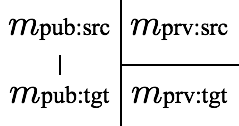
\includegraphics[height=1cm]{figure/memory-0.png}} &
\begin{minipage}{0.5cm}\vspace*{-.8cm}(b)\end{minipage} & 
\fbox{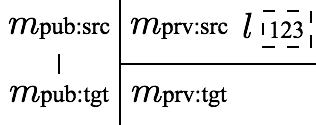
\includegraphics[height=1cm]{figure/memory-1.png}} \\[2mm]
\begin{minipage}{0.5cm}\vspace*{-.8cm}(c)\end{minipage} & 
\fbox{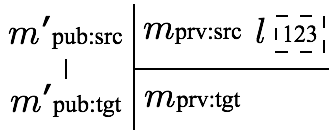
\includegraphics[height=1cm]{figure/memory-2.png}} &
\begin{minipage}{0.5cm}\vspace*{-.8cm}(d)\end{minipage} & 
\fbox{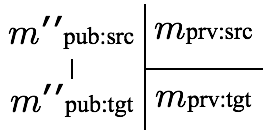
\includegraphics[height=1cm]{figure/memory-3.png}}
\end{tabular}
%
\caption{Memory Invariants for the Running Example}\label{fig:invex}
\end{figure}

We begin at line 1 by assuming the
following conditions on the memory of the source and target programs (see Figure~\ref{fig:invex}~(a)):
\begin{description}
\item[assume] (equivalent arguments) the parameter \texttt{p} contains
  \emph{equivalent} arguments $v_\textrm{src} $ in the source and $v_\textrm{tgt}$ in the target;
\item[assume] (equivalent public memories) 
  there are a set of memory blocks
  $m_\textrm{pub:src}$ in the source and
  $m_\textrm{pub:tgt}$ in the target that are
  \emph{equivalent} and publicly accessible by arbitrary functions;
\item[assume] (source private memory) 
  there is a disjoint set of blocks
  $m_\textrm{prv:src}$ in the source, each of which is
  exclusively owned by a single function;
\item[assume] (target private memory) 
  there is a disjoint set of blocks
  $m_\textrm{prv:tgt}$ in the target, each of which is
  exclusively owned by a single function.
\end{description}
After executing line 1, we add the newly allocated block (call it~$l$) to
the private source memory $m_\textrm{prv:src}$. It is important to note that we can add the
block $l$ to the private source memory because it is a fresh logical
block and thus exclusively owned by \texttt{foo}.  After executing
line 2, the block $l$ contains $123$ (see Figure~\ref{fig:invex}~(b)).

At line 3, we guarantee that the function calls to \texttt{bar} are
\emph{equivalent} as follows:
\begin{description}
\item[guarantee] (equivalent arguments) 
  the arguments $v_\textrm{src}$ and $v_\textrm{tgt}$ to \texttt{bar} are equivalent; 
\item[guarantee] (equivalent public memories) 
  $m_\textrm{pub:src}$ and $m_\textrm{pub:tgt}$,
  which are equivalent and publicly accessible;
\item[guarantee] (source private memory) 
  each location in $m_\textrm{prv:src} \uplus {[l\mapsto 123]}$,
  is exclusively owned by a single function;
\item[guarantee] (target private memory) 
  each location in $m_\textrm{prv:tgt}$
  is exclusively owned by a single function.
\end{description}
%After the calls to \texttt{bar}, 
When the calls to \texttt{bar} return,
we can assume that the new public
memories are equivalent to each other (though they may not be the same as the previous public memories), and
the private memories are untouched (see Figure~\ref{fig:invex}~(c)):
\begin{description}
\item[assume] (equivalent public memories) we have new public memories $m'_\textrm{pub:src}$ and
  $m'_\textrm{pub:tgt}$, which are \emph{evolved} from $m_\textrm{pub:src}$
  and $m_\textrm{pub:tgt}$ (see \S\ref{reasoning:simulation} for the definition of memory evolution), and 
  are equivalent and publicly accessible;
\item[assume] (source private memory) $m_\textrm{prv:src} \uplus
  {[l\mapsto 123]}$ is unchanged;
\item[assume] (target private memory) $m_\textrm{prv:tgt}$ is
  unchanged.
\end{description}

At line 4, we load the value $123$ from the source's private memory and
store it in the variable \texttt{a}.  At line 5, in the source, we
store the value of \texttt{a}, which is $123$, in the memory cell located at
the address $v_\texttt{src}$.  In the target, we store the constant
$123$ in the cell at $v_\texttt{tgt}$. Since we stored equivalent
values at equivalent locations $v_\texttt{src}$ and $v_\texttt{tgt}$,
we will have equivalent public memories $m''_\textrm{pub:src}$ and
$m''_\textrm{pub:tgt}$, while leaving the private memories unchanged.

Finally, we return to the callers of \texttt{foo} with (see Figure~\ref{fig:invex}~(d))
\begin{description}
\item[guarantee] (equivalent public memories) 
  $m''_\textrm{pub:src}$ and $m''_\textrm{pub:tgt}$
  that are evolved from $m_\textrm{pub:src}$ and $m_\textrm{pub:tgt}$,
  and are equivalent and publicly accessible;
\item[guarantee] (source private memory) 
  $m_\textrm{prv:src}$;
\item[guarantee] (target private memory) 
  $m_\textrm{prv:tgt}$,
\end{description}
where we can ignore the block $l$ because it is not going to be used any more.
Note that we here guarantee \text{foo} returns with the same private memories it was given
initially, as we assumed the same property for the function
\texttt{bar} after line 3.

\subsection{Memory Invariants}
\label{reasoning:invariants}

As informally discussed above, we prove program refinement using a memory invariant that places conditions on
public memories (which must be equivalent in the source and target programs) and private memories (which can differ between them).  We now formally define the
notion of memory equivalence used in our informal
example, and the conditions on the private memories.

The idea of memory equivalence is a simplification of CompCert's
memory injection \cite{Leroy-Appel-Blazy-Stewart-memory-v2}.  Our
conditions for concrete blocks are inspired from CompCertTSO's support
for finite memory \cite{vsevvcik2013compcerttso}.  See
\S\ref{sec:discussion} for more comparisons.

%%  in the source and the
%% target are exactly the same because optimizations like DAE may remove
%% memory blocks. Thus, we introduce a more relaxed notion of
%% equivalence.

\paragraph{Memory Equivalence}
We define a more relaxed notion of equivalence than simple equality,
which would be too strong in the presence of (unrelated) private
memories. We say that a set of blocks $m_\textrm{src}$ in the source
is equivalent to a set of blocks $m_\textrm{tgt}$ in the target
when they satisfy the following conditions. First, there should be a
bijection, say $\alpha$, between the block identifiers in
$m_\textrm{src}$ and those in $m_\textrm{tgt}$. Second, corresponding
blocks (\ie those related by $\alpha$) should have the same
size and validity, and the values they hold at each offset should be \emph{equivalent}.  Values are
equivalent (w.r.t. $\alpha$) when either both are the same integer, or
they are logical addresses that are at the same offset in corresponding blocks
(w.r.t.~$\alpha$). When $m_\textrm{src}$ and $m_\textrm{tgt}$ are equivalent in this sense, we write $m_\textrm{src} \simeq_\alpha m_\textrm{tgt}$.

\begin{figure}[t]
\center
  %% \fbox{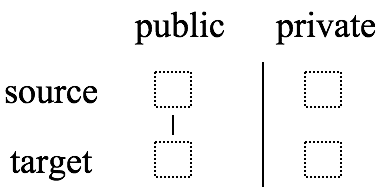
\includegraphics[scale=0.25]{figure/relation-compcert.png}}
  \begin{minipage}[b]{0.28\textwidth}
  \fbox{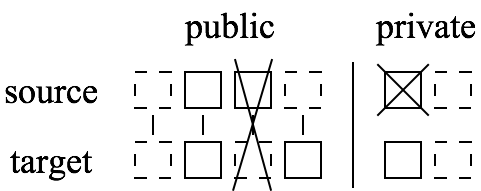
\includegraphics[scale=0.25]{figure/relation.png}}
  \end{minipage}
  \begin{minipage}[b]{0.14\textwidth}
  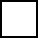
\includegraphics[scale=0.25]{figure/physical-block.png} concrete block\\[2mm]
  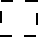
\includegraphics[scale=0.25]{figure/logical-block.png} logical block\\
  \mbox{}
  \end{minipage}
%% (1) for CompCert model, and (2) for our model
\caption{Memory Invariants for Quasi-Concrete Model}\label{fig:invariant}
\end{figure}

The condition on the concrete addresses of corresponding blocks
merits further explanation. We have four possible cases
regarding whether two corresponding blocks are concrete or logical (see the
\emph{public} side of Figure~\ref{fig:invariant}).  The first case in
the figure (\ie source: logical, target: logical) obviously should be
allowed. The second case (\ie source: concrete, target: concrete)
should also be allowed but only when the concrete addresses
coincide. 

The third case (\ie source: concrete, target: logical) should not be
allowed. To allow this case would be to allow the source memory to contain more concrete
blocks than the target, which leads to two problems: $(i)$ an arbitrary
concrete memory access may succeed in the source but fail in the
target; and $(ii)$ a pointer-to-integer cast may raise out-of-memory
in the source but succeed in the target.  In both cases, the target
may have more behaviors than the source, which is disallowed.  On the
other hand, the final case (\ie source: logical, target: concrete) is
allowed because the situation is exactly the opposite: the source may
have more behaviors than the target, which is allowed.

\paragraph{Private Memory}
For blocks in private memories, we have four possible cases
regarding whether the block is in the source or the target, and
whether the block is concrete or logical (see \emph{private} side of
Figure~\ref{fig:invariant}).  All the cases are allowed except for
source private memory blocks that are concrete, for the same reason
that blocks that are concrete in the source and logical in the target are not
allowed in memory equivalence: the source memory should not contain
more concrete blocks than the target memory.

\paragraph{Memory Invariants}
A memory invariant $\beta$ consists of $(i)$ a bijection $\alpha$ between their
block identifiers, $(ii)$ the source's private memory
$m_\textrm{prv:src}$, and $(iii)$ the target's private memory
$m_\textrm{prv:tgt}$. 
%% Recall that we call two memories equivalent when
%% their public sections are equivalent up to the bijection between block
%% identifiers. 
An invariant $\beta=(\alpha, m_\textrm{prv:src}, m_\textrm{prv:tgt})$ 
holds on a pair of memories $m_{\textrm{src}}$ and
$m_{\textrm{tgt}}$ when they contain the private sections $m_\textrm{prv:src}$ and 
$m_\textrm{prv:tgt}$
and some public sections $m_\textrm{pub:src}$ and
$m_\textrm{pub:tgt}$ such that:
%% their public sections
%% are equivalent and they contain the private sections of the
%% invariant. 
%% Formally, memories $m_{\textrm{src}}$ and
%% $m_{\textrm{tgt}}$ are related by a memory invariant $\beta=(\alpha,
%% m_\textrm{prv:src}, m_\textrm{prv:tgt})$ if there exist 
%% public sections $m_\textrm{pub:src}$ and $m_\textrm{pub:tgt}$ that are equivalent 
%% w.r.t.~$\alpha$
  \[\begin{array}{@{}l}
    (m_{\textrm{src}} \supseteq m_\textrm{pub:src} \uplus m_\textrm{prv:src})~\land~
    (m_{\textrm{tgt}} \supseteq m_\textrm{pub:tgt} \uplus m_\textrm{prv:tgt})~\land\\m_{\textrm{pub:src}} \simeq_\alpha m_{\textrm{pub:tgt}}
  \end{array}\]
  where 
%$\equiv_\alpha$ is the equivalence w.r.t. $\alpha$, and 
$\uplus$ and $\subseteq$ are the disjoint union and the subset relation.

\subsection{Proving Simulation}
\label{reasoning:simulation}

We are now ready to present our reasoning principle formally. Our
basic approach is to verify programs via local simulation in the style
of \cite{Hur:2012:MBK:2103656.2103666}.

%\newcommand{\assumedinvariant}[1]{\widehat{#1}}

A function, say \texttt{foo}, in the source and target is locally
simulated if it satisfies the following conditions.  First, consider
a typical lifecycle of the source and target functions:
\begin{center}
\begin{minipage}{0.475\textwidth}
\begin{lstlisting}
foo(|..|) {        foo(|..|) {  //|\fbox{${\beta_\text{s}}$}|
  ...              ...      //|\hspace*{3pt}$\beta_\text{c}\quad{\beta_\text{s}}\!\sqsubseteq\!\beta_\text{c}$|
  bar(..);         bar(..); //|\fbox{${\beta_\text{r}}\quad\beta_\text{c}\!\sqsubseteq\!{\beta_\text{r}} \,\land\, \beta_\text{c}\!=_{\textrm{prv}}\!{\beta_\text{r}}$}|
  ...        $\rightarrow$    ...      //|\hspace*{3pt}$\beta'_\text{c}\quad{\beta_\text{r}}\!\sqsubseteq\!\beta'_\text{c}$|
  gee(..);         gee(..); //|\fbox{${\beta'_\text{r}}\quad\beta'_\text{c}\!\sqsubseteq\!{\beta'_\text{r}} \,\land\, \beta'_\text{c}\!=_{\textrm{prv}}\!{\beta'_\text{r}}$}|
  ...              ...      //|\hspace*{3pt}$\beta_\text{e}\quad{\beta'_\text{r}}\!\sqsubseteq\!\beta_\text{e} \;\land\; {\beta_\text{s}}\!=_{\textrm{prv}}\!\beta_\text{e}$|
}                }
\end{lstlisting}
\end{minipage}
\end{center}
Here boxed conditions are assumed and the others are guaranteed.

First, in \texttt{foo}, unknown functional calls such as
\texttt{bar(..)} and \texttt{gee(..)} should be synchronized (\ie when
the target calls \texttt{bar}, the source should call \texttt{bar} as
well). Note that when a known function is called, the verifier can either step into
the called function and reason about its code, or treat
it as an unknown function call.

Next, at the entry point of \texttt{foo}, we assume that we are given
memories satisfying a given invariant $\beta_\textrm{s}$, and
equivalent arguments w.r.t. the bijection in $\beta_\textrm{s}$.
Then, we execute the code of \textrm{foo} in the source and the target
until the first unknown function call to \texttt{bar(..)}.  Here we have
to show that there is some invariant $\beta_\textrm{c}$ that holds on
the current memories and that the arguments to the function \texttt{bar}
are equivalent w.r.t. the bijection in $\beta_\textrm{c}$.

Here, we also have to show that the current memories are
\emph{evolved} from the memories given initially by showing that the
current invariant $\beta_\textrm{c}$ is a \emph{future invariant} of
the initial one ${\beta_\textrm{s}}$ 
(denoted ${\beta_\textrm{s}}\sqsubseteq\beta_\textrm{c}$).
We say that $\beta_\textrm{c}$ is a future invariant of 
${\beta_\textrm{s}}$ when satisfying the following conditions,
which rule out changes to the memory that cannot be caused 
by the language's operational semantics.  
%% This invariant $\beta_\textrm{c}$ must also be a \emph{future invariant}
%% of ${\beta_\textrm{s}}$ (denoted ${\beta_\textrm{s}}\sqsubseteq\beta_\textrm{c}$), 
%% which rules out changes to the memory that cannot be caused by the language's operational semantics.  
%% More precisely, 
First, the bijection in
$\beta_\textrm{c}$ should include the bijection of ${\beta_\textrm{s}}$ because
logical blocks cannot be removed during execution (a block
becomes invalid rather than removed when it is freed).  Second, the other
conditions on the public memories in ${\beta_\textrm{s}}$ and
$\beta_\textrm{c}$ are that $(i)$ the size of a block does not change
between ${\beta_\textrm{s}}$ and $\beta_\textrm{c}$, $(ii)$ an
invalid block in ${\beta_\textrm{s}}$ cannot become valid in
$\beta_\textrm{c}$, and $(iii)$ a concrete block in
${\beta_\textrm{s}}$ cannot become logical in $\beta_\textrm{c}$.
However, it is important to note that the contents of public memories
can change between ${\beta_\textrm{s}}$ and $\beta_\textrm{c}$ because
the operational semantics allows
%the called function 
to update values in memory.

Then, we consider the case when the unknown function successfully
returns. We can assume that the memories at return time also satisfy some
\emph{future} invariant ${\beta_\textrm{r}}$. We can also
assume that the function \texttt{bar} does not change the private
memories in $\beta_\textrm{c}$ (denoted $\beta_\textrm{c}
=_{\textrm{prv}} {\beta_\textrm{r}}$) because there is no way
for \texttt{bar} to access them in our quasi-concrete model.

We continue through the function, evolving our invariant at non-call steps and performing similar reasoning at other call sites
such as $\texttt{gee(..)}$.  Finally, when \texttt{foo} returns to its caller, we have to
show that there is some \emph{future} invariant $\beta_\textrm{e}$
that holds on the current memories. Furthermore, we have to show that
we did not change the private memories given in
 the initial invariant $\beta_\textrm{s}$ (\ie $\beta_\textrm{s} =_{\textrm{prv}}
\beta_\textrm{e}$). This condition is necessary because, as seen above, we assume that this property holds at the end of any other function call.
In this way, we construct a local simulation proof for the $\texttt{foo}$.


\subsection{Examples}
\label{sec:intptrcast:compiler-verification:examples}

In this section, we show how to verify the examples shown in \S\ref{sec:quasi}.  All
results here are fully formalized in Coq.

\paragraph{Arithmetic Optimization I}

Consider the transformation in Figure~\ref{code:arith1}. If we assume that integer variables only contain integer
values, not logical addresses, the instruction \texttt{a = (a
  - b) + (2 * b - b)} has no effect on the value of \texttt{a} and is equivalent to no
operation, so the optimization is trivially correct. 

How do we know that integer variables only contain
integer values? The straightforward answer is that our language is statically type-checked, as in the LLVM IR. However, the key reason why this is possible
is that in the quasi-concrete model we actually turn logical addresses into integers
when they are cast to \texttt{int}, rather than placing logical addresses in integer
variables. Also, when we load a value from memory to an integer 
variable (resp. a pointer variable), 
if the loaded value is a logical address (resp. an integer value), we raise undefined
behavior (\ie \emph{error}).
In other words, the quasi-concrete model induces a form of dynamic type
checking in languages that use it. This allows us to verify integer
arithmetic optimizations as in this example.
%% and is only a minor
%% inconvenience to the user. If a programmer using the model wants to
%% load a value whose type is unknown, she can load that value to a
%% pointer-type variable (equivalent to a (void *)-type variable in C)
%% and cast it to whatever type she wants.  Since the pointer type
%% contains both integer values and logical addresses, a load to a
%% pointer-type variable will always succeed.

\paragraph{Dead Code Elimination}

Consider the transformation in Figure~\ref{code:dce}.  This example
is similar to the previous one.  Since we can assume that integer-typed
variables contain only integers, the execution of the call
\texttt{foo(a)} does not have any side effects.
Furthermore, because we know the code of the function
\texttt{foo}, we do not need to treat it as an unknown function call.
Rather, we just step into the code of the function \texttt{foo} and
execute it in the source.%  In this way, we can easily verify this
% transformation.

\paragraph{Ownership Transfer}

Consider the transformation in Figure~\ref{code:ownership}.  This
example is similar to the running example in
\S\ref{reasoning:running}.

Assume that the first invariant below holds before the \texttt{malloc}.  After
allocating blocks $l_\text{s}$ in the source and $l_\text{t}$ in
the target, and storing 123 in both blocks, we can move the blocks $l_\text{s}$
and $l_\text{t}$ into the private sections of the invariant because they are logical and disjoint from the
public sections, yielding the second invariant below. Next we call the function \texttt{bar}. When it
returns, we can assume that the third invariant holds (\ie the
private sections are untouched). After loading, the variable
\texttt{a} will contain 123, since \texttt{p} contains the
logical address $(l_\text{s},0)$ in the source and $(l_\text{t},0)$ in
the target. 

Next, when we call \texttt{hash\_put}, we have to make sure that the
arguments are equivalent. The first arguments are equivalent because
we assume that we start with equivalent values in variables, and the third arguments
are equivalent because \texttt{a} contains 123.  To show that
the second arguments, $(l_\text{s},0)$ and $(l_\text{t},0)$, are
equivalent, we move the blocks from the private sections to the public
section and extend the bijection $\alpha'$ to relate $l_\text{s}$
and $l_\text{t})$ (the fourth invariant below). Such ownership
transfer from the private sections to the public section is allowed
because the future invariant relation ($\sqsubseteq$) requires
only the bijection to be non-decreasing, not the private
sections.
\begin{center}
\fbox{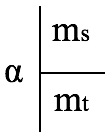
\includegraphics[scale=0.25]{figure/ownership-0.png}}\hfill
\fbox{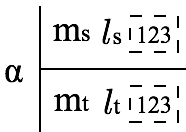
\includegraphics[scale=0.25]{figure/ownership-1.png}}\hfill
\fbox{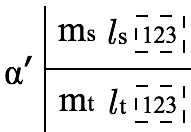
\includegraphics[scale=0.25]{figure/ownership-2.png}}\hfill
\fbox{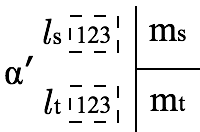
\includegraphics[scale=0.25]{figure/ownership-3.png}}
\end{center}

% \begin{lstlisting}
% foo(int i) {
%   var ptr p, ptr q, int r;
%   p = malloc (1);
%   q = malloc (10);
%   3 -> p;
%   5 -> q + i;
%   bar();
%   r <- p;
%   goo(r, (int) p);     $\to$ goo(3, (int) p);
% }
% \end{lstlisting}

% \begin{itemize}
% \item \texttt{p} is known to contain \texttt{3}, so we replace a use
%   of \texttt{r} by \texttt{3}.
% \item We can perform constant propagation optimization to this example
%   even though 1) there is a store to another block (\texttt{q})
%   between the store to and the load from \texttt{p}, 2) there is an
%   function call to an unknown function \texttt{bar} between the store
%   and the load, and 3) the exclusive ownership of \texttt{p} is lost
%   after the load from \text{p}.  Since \texttt{p} is allocated as a
%   logical block, can mark \texttt{p} as private.  Thus \texttt{r}
%   should be \texttt{3} after the function call to \texttt{bar}.
% \item If a pointer is determinted to be physical or logical at the
%   allocation time, this example is not justified due to ownership
%   transfer.  Since \texttt{p} is casted to integer, it should be
%   allocated at a physical address.  Thus \texttt{p} should be marked
%   as public, and \texttt{bar} may modify the content of \texttt{p}.
% \end{itemize}


\paragraph{Arithmetic Optimization II}

We can easily verify the transformation in Figure~\ref{code:arith2}
for the same reason as in \S\ref{ex:arith1}: because we can assume
that all integer variables contain integer values.

% \begin{itemize}
% \item Thanks to elaboration, we know the type of operands of every
%   operation.  For example, we can distinguish integer additions based
%   on the type of operands ($\texttt{+}_{\mathtt{ii}}$ between two
%   integers, $\texttt{+}_{\mathtt{pi}}$ between a pointer and an
%   integer, and $\texttt{+}_{\mathtt{ip}}$ between an integer and a
%   pointer).
% \item Standard integer optimizations are justified in our model, as
%   integer variables really contain integer values, not logical
%   pointers.  For instance, the above optimization is justified in our
%   model: the source program that require 4 integer operations into the
%   target program that require 3 integer operations.
% \item However, this optimization is not justified in the CompCert
%   model.  Suppose \texttt{a} contains an integer, and \texttt{b0},
%   \texttt{b1} and \texttt{b2} contain logical pointers of the same
%   block.  Since \texttt{a - b0} is \texttt{Vundef}, the operands of
%   two \texttt{printf}'s in the target are unconstrained, while those
%   of the source are specific integers.
% \end{itemize}

\paragraph{Dead Cast Elimination}

Consider the transformation in Figure~\ref{code:deadcast}, in the case in which
the source uses the quasi-concrete model and the target uses the
concrete model.

We begin by assuming that the first invariant below holds before the call to
\texttt{foo}, where the variable \texttt{p} contains equivalent
addresses $(l_\text{s},i)$ in the source and $\toint{(l_\text{t},i)}{m}$ in the target.
Note that the block $l_\text{t}$ is concrete, since the target is using
the fully concrete model. After the allocation of a block, say
$l'_\text{s}$, in \texttt{foo} in the source, we move it to the source's
private memory, yielding the second invariant below.  Here it is important
to note that if the source was using the concrete model, we could not move
the block $l'_\text{s}$ into the private section because $l'_\text{s}$
would be concrete, which would invalidate our proof.

After the cast, the block $l_\text{s}$ becomes concrete, yielding the third
invariant below.  Here it is important to note that if the target
language was using the quasi-concrete model and $l_\text{t}$ were logical,
then we would produce an invariant in which $l_\text{s}$ is
concrete and $l_\text{t}$ is logical, which would be an invalid invariant.  After
\texttt{foo} returns, we simply drop the block $l'_\text{s}$ from the
source private section because we do not use it, yielding the fourth
invariant below. Then we can proceed to verify the rest of the code.
\[
\fbox{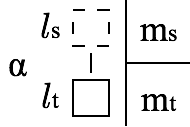
\includegraphics[height=.95cm]{figure/deadcast-0.png}}\,
\fbox{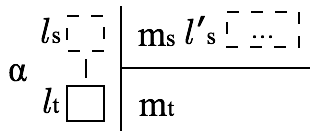
\includegraphics[height=.95cm]{figure/deadcast-1.png}}\,
\fbox{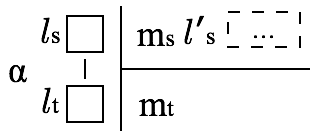
\includegraphics[height=.95cm]{figure/deadcast-2.png}}\,
\fbox{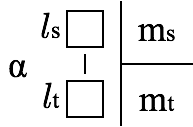
\includegraphics[height=.95cm]{figure/deadcast-3.png}}
\]

\paragraph{Identity Compilers}
As a sanity check for our reasoning principles, we wrote an identity compiler from our language with the quasi-concrete
model to itself, and a simple compiler from our language with the quasi-concrete
model to the same language with the concrete model. The latter compiler just eliminates
dead casts of the form ${\texttt{\_ = (int) p}}$. We successfully verified these two compilers in Coq using our reasoning principles.

% \begin{tabular}{ll}
% \small
% \begin{lstlisting}
% foo(int i) {
%   var ptr p, int r;
%   p = malloc (10);
%   3 -> p + i;
%   bar();
%   r <- p + i;
%   free (p);
% }
% \end{lstlisting}
% \begin{lstlisting}
% foo(int i) {



%   bar();


% }
% \end{lstlisting}
% \end{tabular}

% \begin{itemize}
% \item If a block is not physically realized, then we can optimize as
%   in the logical model.  In the above example, we can optimize out
%   everything related to the memory block allocated at \texttt{p}.
% \end{itemize}

% \begin{tabular}{ll}
% \begin{lstlisting}
% foo(ptr p) {
%   var int i;
%   i = (int) p;
%   bar(i);
% }
% \end{lstlisting}
% \begin{lstlisting}
% bar(int i) {
%   var int j;
%   j = i * 3;   $\to$ skip
% }
% \end{lstlisting}
% \end{tabular}

% \begin{itemize}
% \item In our model, this example is justified.  Since casting to
%   integer requires pointers to take physical address, \texttt{i}
%   contains an integer, not a logical pointer.  Thus we can optimize
%   out the multiplication without worrying about side effects.
% \item In the CompCert model, casts between integers and pointers are
%   ignored, and integer variables may contain logical pointer values.
%   When an operation require an integer but a logical pointer is given,
%   CompCert return \texttt{Vundef} (undefined value). 
% \item \todo{What is the point of this example?}
% \end{itemize}


%%% Local Variables:
%%% mode: latex
%%% TeX-master: "main"
%%% TeX-command-extra-options: "-shell-escape"
%%% End:

\section{Discussion}
\label{sec:intptrcast:discussion}

\subsection{Implementation and Experiment Details}

\paragraph{Coq Formalization}
All the proofs reported in this paper have been fully formalized in
Coq and can be found in the project webpage.  Our Coq formalization is about 10,000 lines of code,
excluding empty lines and library code.  The formalization took about 2
person-months to complete.

\paragraph{Optimization Examples}
All optimization examples presented in the paper are performed by Clang
3.4.2 and/or GCC 4.8.3.  Examples in C and their compilation
results can be found in the project webpage.


\subsection{Related Work on Formal Semantics}

\paragraph{Formal Memory Models}
There have been numerous efforts to formalize C semantics, both from
the perspective of clarifying the specification and defining
implementations with formal semantics~\cite{norrish1998c,leroy:compcert,ellison2012executable,krebbers2011formalization,Greenaway:2014:DSS:2594291.2594296}. These invariably use
variations of the logical memory model, where each allocation is
associated with some abstract identifier and pointers consist of
an identifier and some path representing an offset into the memory
block, except for the work of Norrish~\cite{norrish1998c} which uses the concrete model.

\paragraph{Comparison with CompCert}
CompCert~\cite{leroy:compcert,Leroy-Appel-Blazy-Stewart-memory-v2} and its various extensions
currently allow casting pointers to and from integers, but the
semantics preserves the logical representation of pointers after the cast. 
As a result, integer variables can contain not only normal 32-bit integers,
but also logical pointer representations.
In the higher-level languages (CompCert C and Clight), performing arithmetic
on cast pointer is treated as a program error, whereas in the low-level languages
(from Cminor down to assembly), adding and subtracting integer values 
from converted pointers is defined and affects only the offset into the pointer's 
logical block. There
has also been work on extending the semantics to support pointer
fragments to allow, for example, \code{memcpy} to work on memory
containing pointers~\cite{krebbers2014formal}, but these extensions still cannot fully 
support arithmetic operations on pointer values that have been cast
to an integer type.

\paragraph{Comparison with CompCertTSO}
The CompCertTSO compiler~\cite{vsevvcik2013compcerttso} extends CompCert's
Clight language with threading and atomic memory primitives following the
x86-TSO relaxed memory model. Similar to us, CompCertTSO's memory model 
also supports finite memory, but uses a different mechanism to do so.
It has a distinguished logical block, where the offset serves as essentially a
concrete memory address. 
%In addition to the operations on pointers defined
%under CompCert's Clight semantics, in CompCertTSO pointer equality is always
%defined within the same block. 
During compilation, all memory operations are
lowered to act only on a single finite logical block. This allows the source
and target languages, with infinite and finite memory respectively, to share a
single memory model, and simplifies the correctness statements by removing
the need for CompCert's memory injections. 
%We can replicate this behavior by having a fully concrete semantics, where
%all pointers become realized immediately upon allocation.
CompCertTSO handles pointer-integer casts in the same way as CompCert, with the same limitations.

\paragraph{Comparison with the Symbolic Value Approach}
Most recently, Besson et al. have proposed an extension to CompCert's
memory model that gives semantics to bit-masking operations on
pointers and uninitialized values~\cite{besson2014precise}. Their
approach involves adding lazily-evaluated symbolic expressions,
including arbitrary operations on the representation of pointers, to
the class of semantic values. Symbolic values are forced whenever a
concrete value is needed to take a step, for example to access memory
through a pointer or in the guard of a conditional. The mapping is
performed by a normalization function given as a parameter of the
semantics. The normalization function is partial, and is only defined
precisely when the symbolic value evaluates to a unique result under
every assignment from logical block identifiers to concrete addresses
(subject to some validity conditions).
% This is done using an auxiliary
% low-level semantics for expressions in which pointers and integers
% have the same representation.

The semantics of Besson et al. is necessarily deterministic: non-determinism is
interpreted as undefined behavior, while our model
captures the non-deterministic allocation of concrete addresses.
Furthermore, their semantics is complex and indeed intractable: their
normalization is implemented with an SMT solver, and the semantics in general is too complex to serve as a mental model for ordinary C programmers. Normalization in our semantics,
on the other hand, is a straightforward translation from
pointers to concrete blocks and integers.

Most importantly, while their approach gives semantics to non-strictly-conforming C programs
involving bit-masking of pointers and uninitialized values, it fails to define useful programs that
use integer-pointer casts.  Consider the \code{hash\_put} example discussed in
\Cref{sec:intptrcast:formal-semantics:ownership}, where a pointer is hashed and then presumably used
to index into an array.  Since the resulting memory location will depend on the concrete layout of
memory, the resulting program will have undefined behavior in their semantics.  In general, any
program that displays non-determinism due to the concretization of pointers in our model is necessarily
undefined in Besson et al.'s model.

% the model of Besson et al. Furthermore, it
% is not possible to extend their model to support these cases since
% determinism is required for the correctness of their semantics: memory
% only contains logical pointers and concrete realizations are
% enumerated independently at each normalization step. Allowing
% non-determinism would allow contradictory observations about the
% physical layout of memory. Supporting concrete pointers in memory is
% essential to ``remember'' previous decisions about the realization of
% logical pointers. Finally, we contend that their model fails to allow
% simple reasoning by the user.


\subsection{Compatibility}

\paragraph{Compatibility with Other C Language Features}

There are numerous other C language features that have some
interaction with the memory model.  Some of them, such as
\textit{indeterminate values} \cite[\S3.19.2p1]{c18}, \textit{dangling pointers}
\cite[\S6.2.4p2]{c18}, and \textit{infinite loops with no side-effects}
\cite[\S6.8.5p6]{c18}, have semantics that are largely orthogonal to
the pointer concretization used in our hybrid model.
Similarly, our model explicitly allows \textit{unsafely-derived pointers},
which are permitted in C18 and implementation-defined in C++17 \cite[\S6.6.4.4.3]{c++17}.
We allow them in order to support low-level programming idioms such as XOR linked lists and
compressed oops in HotSpot JVM.

Our paper does not directly address threads, so we cannot claim with
certainty that the model extends to handle them.  However, we see no
obstacles in this direction, and the hybrid model is similar
to CompCertTSO, which does support a weak memory model and threads, so
we are optimistic that this extension to the semantics should follow similarly.

A few language features require some adaptation of our memory model.
For instance, we can adapt the hybrid model to support
\textit{union types} and \textit{strict aliasing}, following Krebbers'
technique~\cite{krebbers2013aliasing}, which works regardless of
whether the model is concrete, logical or hybrid.

As another example, in C, \code{char*} is a ``universal'' pointer type, which allows
efficient bulk data moves via \code{memcpy}.  Krebber's variant of
CompCert~\cite{krebbers2014formal} already supports this semantics using a logical
memory, and the hybrid model is compatible with that solution.
Briefly: we let \code{char} types store byte-indexed logical values
(such as $(l,10)\!:\!2$, which denotes the second byte of the logical
address $(l,10)$). This strategy works because a \code{char} is
implicitly cast to an integer when used in arithmetic operations,
and thus we
can simply treat these casts as side-effecting (\textit{i.e.},
concretizing the logical addresses).  This approach lose (almost) no
optimization opportunities because byte-indexed logical addresses
are typically loaded from the memory and 
thus (mostly) already treated as public by the compiler.


% *** What is the role of our model?

% We intend to use our model to build a verified translation validation
% framework for LLVM (eventually) supporting all C features used in
% practice.  Cleanly modeling pointer-to-integer casts is a necessary
% step toward this goal.  With this application in mind, we strived to
% make the model simple (necessary for proving correctness of
% optimizations) yet permissive (allowing us to justify many
% optimizations).

% Our model is not intended to be a replacement for the C standard;
% rather it is the specification of a particular compiler implementation
% that refines the standard.

% *** Can our model evolve to an actual language spec?

% We believe that our model can be extended to support all practically
% used features of C, and that all these extensions are orthogonal to
% the realization of pointers we propose.  Here we elaborate on them.

% 1. Unsafely-derived pointers. 
% They are allowed in C11 and implementation-defined in C++11 [C++11
% 3.7.4p4]. We chose to allow them in order to support low-level
% programming idioms such as XOR linked lists and compressed oops in
% HotSpot JVM.  (Disallowing them would enable garbage collection in
% C/C++, which is rare.)

% 2. Threads \& Concurrency.
% Our paper does not directly address threads, so we cannot claim with
% certainty that the model extends to handle them.  However, we see no
% obstacles in this direction, and our model is similar to CompCerTSO,
% which does support a weak memory model and threads, so we are
% optimistic that this should be straight forward.

% 3. Char*/memcpy
% A variant of CompCert [with Krebber's patch, in github] already
% supports char*/memcpy in logical memory, and our model is compatible
% with that solution.  Briefly: we let char types store logical values
% (eg, such as (l,10):2 denoting the second byte of the logical address
% (l,10)). This is OK because chars are implicitly cast to integers by
% arithmetic operations. We can simply treat these casts as
% side-effecting (ie, realizing any logical addresses). Here, we lose
% (almost) no optimization opportunities by realizing such logical
% addresses because they are stored in the memory and thus (mostly)
% already treated as public by the compiler.

% 5. 
% *** Applicability to existing verified compilers?

% We believe that our ideas are readily applicable to CompCert(TSO) and
% related projects like Vellvm because our memory model and notion of
% memory invariant are technically very close to CompCert's. (Vellvm
% also uses CompCert's memory model.) Essentially, all that would have
% to change in the proofs are the cases handling pointer to integer
% casts.

\paragraph{Compatibility with Alias Analyses} The hybrid model is largely
compatible with common alias analyses.  For instance, it can be used
to justify \textit{size-based alias analysis}, which considers
pointers to differently-sized objects as distinct. For example, in
the code below, there is no alias between \code{p} and \code{q}:
even if \code{q} points to the block
pointed to by~\code{p}, loading or storing a double value in the
block will fail since the block is not big enough to contain double
values.
\begin{center}
  \begin{minted}{c}
    int *p = malloc(sizeof(int));
    double *q = foo(p);    // no alias between p and q
  \end{minted}
\end{center}

It also justifies %(modulo the effects of cast)
\textit{freshness-based alias analysis}, which assumes that the result of
\code{malloc} is distinct from all other pointers.  The 
following example of constant propagation is valid in the
hybrid model since \code{q} points to a fresh block that
is different from the block pointed to by \code{p}.
It is important to note that there is no alias
between \code{p} and \code{q} even after
the fresh block is concretized. The reason is because
even if \code{p} and \code{q} may be cast to the same integer,
they still point to different blocks as pointer values.
%% However, uncommenting the cast
%% invalidates the transformation because  \code{p} might happen to point
%% to the realized physical address of \code{q}. In practice, such cast
%% pointer values are usually global and passed to other functions, such
%% as \code{hash\_put} (as shown in the second comment). In
%% such cases, neither GCC nor Clang performs the constant propagation.
\begin{center}
\begin{tabular}{@{}l@{}l@{~~}l}
\small
\begin{minipage}{0.45\textwidth}
\begin{minted}{c}
void foo(int *p) {
  auto q = (int *) malloc(4);
  auto a = (uintptr_t) q;
  auto b = *p;
  *q = 123;
  auto r = *p;
}
\end{minted}
\end{minipage}
&
$~\rightarrow$
&
\small
\begin{minipage}{0.45\textwidth}
\begin{minted}{c}
void foo(int *p) {
  auto q = (int *) malloc(4);
  auto a = (uintptr_t) q;
  auto b = *p;
  *q = 123;
  auto r = b;         // CP
}
\end{minted}
\end{minipage}
\end{tabular}
\end{center}




\subsection{Impact}

In the course of doing this research, we discovered the GCC bug presented in
\Cref{fig:introduction:bug}.  With this bug, we persuaded compiler writers that $(1)$ it is subtle
to define the semantics of casts between pointers and integers, and $(2)$ it is safe to turn off
some alias analyses that are too aggressive to peacefully coexist with other optimizations.

Our idea to give semantics to more programs involving pointer operations---namely, using concrete
and logical blocks at the same time---has subsequently been refined by follow-up papers by other
researchers~\cite{intptrcast-oopsla,intptrcast-popl}, which are accompanied with promising revision
proposals to the LLVM compiler and ISO C standard.

% The hybrid model refines the C standard by giving semantics to more programs involving pointer
% operations.

We intend to use this model for compiler verification tasks, extending the range of common
optimizations that can be verified.  Ultimately, we would like to generalize
Crellvm~\cite{crellvm}---the credible compilation framework for LLVM---to support casts between
pointers and integers.  We would also like to integrate our model with CompCert and use it to
justify new CompCert optimizations.  We believe that our ideas are readily applicable to
CompCert(TSO) and related projects like Vellvm~\cite{vellvm:popl12,vellvm:pldi13} because our memory
model and notion of memory invariant are technically very close to CompCert's.  (Vellvm also uses
CompCert's memory model.)  Essentially, all that would have to change in the proofs are the cases
handling pointer to integer casts.

% all commonly-used features of C.


%% 

% \paragraph{Conclusion and Future Work}
% Future work 1: Revising CompCert in our way requires a lot of overhead? \cite{leroy:compcert}

% Conclusion: our model applies to C, LLVM IR and CompCert(TSO).


%%% Local Variables:
%%% mode: latex
%%% TeX-master: "main"
%%% TeX-command-extra-options: "-shell-escape"
%%% End:



\chapter{Epilogue}
\label{chap:epilogue}

\section{Conclusion}
\label{sec:conclusion}

\paragraph{Genesis}

The genesis of this dissertation traces back to 2014, when my supervisor Prof. Chung-Kil Hur ran a
seminar on CompCert~\cite{compcert}.  CompCert is exciting because it demonstrated formal semantics
and compiler verification research scale up to real-world applications.  One day, he asked what are
the concrete addresses of global variables in CompCert C, and I answered ``I don't know.''  So we
read CompCert code together, and realized that CompCert C does not assign concrete addresses to
global variables because it does not support cast between integers and pointers.  Then we started to
develop a formal semantics of the feature, which ended up being my first first-author
paper~\cite{intptrcast}.

It was exciting to advance the state-of-the-art of C formal semantics, and it naturally became my
dissertation topic.  I focused on low-level features because they are difficult to capture in a
formal semantics due to the conflict among many ``stakeholders.''  To understand them, I began to
read C/C++ standards, Linux kernel and LLVM mailing lists, and even architecture ISA manuals which I
didn't expect to do so at the beginning of my graduate school life.



\paragraph{Contributions}

As a result, we developed formal semantics of three low-level features of C crucially used in
systems programming, namely relaxed-memory concurrency, separate compilation, and cast between
integers and pointers.  Our semantics adequately balances the conflicting desiderata of programmers,
compilers, and hardware in that it $(1)$ supports the features' common usage patterns and reasoning
principles for programmers, and $(2)$ provably validates major compiler optimizations at the same
time.  To establish confidence in our formal semantics, we have formalized most of our key results
in Coq.


\paragraph{Impact}

Our formal semantics had concrete impacts on both academia and industry.  In academia, we and others
published follow-up papers that $(1)$ refine our semantics to account for more usage patterns and
compiler optimizations, $(2)$ provide more evidences that show our semantics serves programmers,
compilers, and hardware well, or $(3)$ apply the key idea of our semantics to other languages.  In
industry, $(1)$ we discovered bugs and proposed fixes to bugs in GCC, LLVM, and CompCert, $(2)$ we
provided informed opinions to the discussion on C/C++ and LLVM IR language standards, and $(3)$ our
verification technique was adopted in CompCert.



\paragraph{Future Work}

However, by Meyer's standard, where real success is ``changing the way the IT industry develops
software'', ``the story told in this article is one of glaring, unremitted and probably definitive
failure''~\cite{bertrand-meyer}.  CompCert is changing the way safety-critical softare is
developed~\cite{compcert-avionics,compcert-nuclear}.  In the similar spirit, we would like our
semantics to help system programmers, thereby changing the way systems are developed.  To this end,
we would like to pursue the following directions for future work.

\jeehoon{conclusion: future work}

- relevance
- tools (bug-finder, verifier, logic, ...)
- standardization



% As future work, by further pursuing the research agenda for the formalization of real-world practice
% of C semantics and compilers, we aim to provide clear, theoretically-informed, and
% practically-relevant C semantics and compilers that system programmers can immediately benefit from.
% If successful, our formal semantics will be able to replace the C dialects used in Linux and other
% systems.


%%% Local Variables:
%%% mode: latex
%%% TeX-master: "main"
%%% End:



% \appendix

% \chapter{Technical Appendix}

% \section{Coq Formalization}
\label{sec:coq}

\jeehoon{Write on Coq?}


%%% Local Variables:
%%% mode: latex
%%% TeX-master: "main"
%%% End:



\bibliographystyle{abbrv}
\bibliography{references}

\keywordalt{C, 실행의미, 컴파일러, 정형검증}
\begin{abstractalt}
  \noindent TODO
\end{abstractalt}

%%% Local Variables:
%%% mode: latex
%%% TeX-master: "main"
%%% End:



\end{document}

%%% Local Variables:
%%% mode: latex
%%% TeX-master: "main"
%%% TeX-command-extra-options: "-shell-escape"
%%% End:
